\documentclass[a4paper,10pt,twoside, openright]{book}
\usepackage[english]{babel}
%\usepackage[utf8]{inputenc}
\usepackage{indentfirst}
\usepackage{graphicx}
\usepackage{epigraph}
\usepackage{atlasphysics}
\usepackage{subfigure}
\usepackage{subfloat}
\usepackage{lineno}
\usepackage{setspace}
\newcommand{\AC}{\ensuremath{\text{A}_{\text{C}}}}
\newcommand{\formatGenerator}[1]{\textsc{#1}}
\newcommand{\mcnlo}{\formatGenerator{mc@nlo}}
\newcommand{\wjets}{\ensuremath{W+\mathrm{jets}}}
\providecommand{\abs}[1]{\lvert#1\rvert}
\newcommand{\dy}{\ensuremath{\Delta{}\abs{y}}}
\newcommand{\deta}{\ensuremath{\Delta{}\abs{\eta}}}
\newcommand{\mtt}{\ensuremath{m_{\ttbar{}}}}
\newcommand{\Nupup}{\ensuremath{N(\uparrow\uparrow)}}
\newcommand{\Ndodo}{\ensuremath{N(\downarrow\downarrow)}}
\newcommand{\Nupdo}{\ensuremath{N(\uparrow\downarrow)}}
\newcommand{\Ndoup}{\ensuremath{N(\downarrow\uparrow)}}


\newcommand\myskip{\vspace{\baselineskip}}
\def\Xbar{\ensuremath{\bar{X}}}
\def\XXbar{\antibar{X}}
\def\Ybar{\ensuremath{\bar{Y}}}
\def\YYbar{\antibar{Y}}
\def\Tbar{\ensuremath{\bar{T}}}
\def\TTbar{\antibar{T}}
\def\Bbar{\ensuremath{\bar{B}}}
\def\BBbar{\antibar{B}}
\newcommand\TT{\ensuremath{T\bar{T}}}
\newcommand\BB{\ensuremath{B\bar{B}}}
\newcommand\T{\ensuremath{T}}
\newcommand\B{\ensuremath{B}}
\newcommand{\TB}{\ensuremath{(T \, B)}}
\newcommand{\XT}{\ensuremath{(X \, T)}}
\newcommand{\BY}{\ensuremath{(B \, Y)}}
\def\Tlr{\ensuremath{T_{L,R}}}
\def\Blr{\ensuremath{B_{L,R}}}
\def\Ylr{\ensuremath{Y_{L,R}}}
\def\Xlr{\ensuremath{X_{L,R}}}
\def\TBlr{\ensuremath{\TB_{L,R}}}
\def\BYlr{\ensuremath{\BY_{L,R}}}
\def\XTlr{\ensuremath{\XT_{L,R}}}
\def\vlt{vector-like top partner}
\def\vlb{vector-like bottom partner}

%%%%%%%%%%%%%%%%%%%%%%%%
%%% LAZYNESS-DRIVEN DEFS
%%%%%%%%%%%%%%%%%%%%%%%%
\def\cme{center-of-mass energy}
\def\cmm2{cm$^{-2}$}
\def\sm1{s$^{-1}$}
\def\chisq{$\chi^2$}
\def\loose{{\sc Loose}}
\def\tight{{\sc Tight}}
\def\whad{\ensuremath{W_{\rm had}}}
\def\wlep{\ensuremath{W_{\rm lep}}}
\def\wi{$W_{\rm had}^{\rm type\;I}$}
\def\wii{$W_{\rm had}^{\rm type\;II}$}
\def\mreco{\ensuremath{m_{\rm reco}}}
\def\chii{{\sc ``{\small 2 \btag ged jets}''}}
\def\chiii{{\sc ``{\small 3 \btag ged jets}''}}
\def\chiv{{\sc ``{\small{\footnotesize$\geq$}4 \btag ged jets}''}}

\def\dr{\ensuremath{\Delta R}}
\def\OR{\texttt{OR}}
\def\AND{\texttt{AND}}
%\def\bjet{$b$jet}
\def\bjet{$b$-jet}
%\def\cjet{$c$jet}
\def\cjet{$c$-jet}
\def\ljet{light-jet}
\def\btag{$b$-tag}
\def\ctag{$c$-tag}
\def\mt{\ensuremath{m_T}}
\def\mtw{\ensuremath{m_T(W)}}
\def\wbx{\ensuremath{\TTbar\to Wb+X}}
\def\htx{\ensuremath{\TTbar\to Ht+X}}
\def\nontt{non-$t\bar{t}$}
\def\mclimit{\texttt{MCLimit}}
\def\cls#1{\ensuremath{CL_{\rm #1}}}
\def\hthad{\ensuremath{H_T^{\rm had}}}
\def\htfj{\ensuremath{H_T^{4j}}}
\def\tthf{\ttbar+HF}
\def\ttlf{\ttbar+light}

\def\bra#1{\mathinner{\langle{#1}|}}
\def\ket#1{\mathinner{|{#1}\rangle}}
\def\braket#1{\mathinner{\langle{#1}\rangle}}
\def\Bra#1{\left<#1\right|}
\def\Ket#1{\left|#1\right>} 
\newcommand{\Overline}[2][1]{%
  {}\mkern#1mu \overline{\mkern-#1mu #2 \mkern-#1mu}\mkern#1mu {}} 
\DeclareMathAlphabet{\mathpzc}{OT1}{pzc}{m}{it}


\linespread{1.2}                        %comando per impostare l'interlinea
\usepackage{feynmf}
\usepackage{psfrag}
\usepackage[usenames,dvipsnames,svgnames,table]{xcolor}
\definecolor{light-gray}{gray}{0.9}
\usepackage{pgf,pgfarrows,pgfnodes}
\usepackage{dcolumn}
\usepackage{afterpage}

\newcolumntype{x}[1]{%
>{\centering\arraybackslash}m{#1}}%


\usepackage[percent]{overpic}


\newcommand{\nocontentsline}[3]{}
\newcommand{\tocless}[2]{\bgroup\let\addcontentsline=\nocontentsline#1{#2}\egroup}

%\usepackage{ulem} %sostituisce l'effetto sottolineatura all'effetto corsivo nel comando \emph{} e risolve il problema delle righe che non si spezzano

\usepackage{multirow,bigdelim}
\usepackage{enumerate}

\usepackage[hdivide={3cm, *, 3cm}, vscale=0.75]{geometry}
\usepackage{chngpage}

\usepackage[margin=7pt,font=small,labelfont=bf]{caption}
%\usepackage[margin=10pt,font=small,labelfont=bf]{caption}
%\usepackage[format=hang,indention=-2cm,labelfont=bf]{caption}%per delle caption più carine
\usepackage{booktabs}
\usepackage{longtable}
%\usepackage{pdflscape} 
%\usepackage[pdftex]{lscape}
\usepackage{lscape}
\usepackage{slashed}

\usepackage{listings}
\lstset{language=C}

\hyphenation{ca-lo-ri-me-ter ca-lo-ri-me-ters}%serve per la sillabazione: tra parentesi 

\setlength{\headheight}{15pt}
\usepackage{pict2e}
%\usepackage{guit}

%\usepackage{natbib}
%\bibliographystyle{unsrt}
%\usepackage[babel]{csquotes}
%\usepackage[style=numeric,sorting=none]{biblatex}
%\bibliography{biblio}


%MATHS
\usepackage{amssymb}
\usepackage{amsmath}
\usepackage{latexsym}
\usepackage{amsthm}
 \newcommand{\sgn}{\mathop{\mathrm{sgn}}}
\usepackage{slashed}

%\usepackage[T1]{fontenc}
%\usepackage{microtype}

\usepackage{fancyhdr}
\pagestyle{fancy}

\usepackage{eso-pic}

\usepackage{url}
%%%%bookmarksnumbered=false,% true means bookmarks in left window are numbered
%%%%dvips,%ps2pdf,
%%%%bookmarksopen=false, % true means only level 1 are displayed.
%\usepackage[ocgcolorlinks,bookmarks=true,bookmarksnumbered=false,bookmarksopen=false,colorlinks=true,linkcolor=webred]{hyperref}
\usepackage[bookmarks=true,bookmarksnumbered=false,bookmarksopen=false]{hyperref}
%\usepackage[pdfborder={0 0 0 0}]{hyperref}
\definecolor{webgreen}{rgb}{0, 0.5, 0} % less intense green
\definecolor{webblue}{rgb}{0, 0, 0.5} % less intense blue
\definecolor{webred}{rgb}{0.5, 0, 0} % less intense red

%END OF PACKAGES

%per includere il frontespizio (ottenuto in pdf a parte)
\newcommand\BackgroundPic{
\put(0,0){
\parbox[b][\paperheight]{\paperwidth}{%
\vfill
\centering

\includegraphics[width=\paperwidth,height=\paperheight,
keepaspectratio]{smallstuff/frontespizio}%
\vfill
}}}



%per avere l'indice senza numeri di pagina
\makeatletter 
 \newcommand{\cleantableofcontents}{% 
   \clearpage\begingroup 
   \let\ps@plain\ps@empty\pagestyle{empty}% 
   \tableofcontents\clearpage\endgroup} 
 \makeatother

%per lo stile dei capitoli
\makeatletter
\def\thickhrulefill{\leavevmode \leaders \hrule height 1ex \hfill \kern \z@}
%chstyle
\def\@makechapterhead#1{%
  \vspace*{10\p@}%
  {\parindent \z@ 
    {\raggedleft \reset@font
      \scshape \@chapapp{} \thechapter\par\nobreak}%
    \par\nobreak
    \vspace*{30\p@}
    \interlinepenalty\@M
    {\begin{spacing}{1.1} \raggedright \huge \bfseries #1\end{spacing}}%
    %{\doublespacing \raggedright \huge \bfseries #1}%
    \par\nobreak
    \hrulefill
    \par\nobreak
    \vskip 90\p@
  }}
\def\@makeschapterhead#1{%
  \vspace*{10\p@}%
  {\parindent \z@ 
    {\raggedleft \reset@font
      \scshape \vphantom{\@chapapp{} \thechapter}\par\nobreak}%
    \par\nobreak
    \vspace*{30\p@}
    \interlinepenalty\@M
    {\begin{spacing}{1.1} \raggedright \huge \bfseries #1\end{spacing}}%
    \par\nobreak
    \hrulefill
    \par\nobreak
    \vskip 90\p@
  }}



\renewcommand{\chaptermark}[1]{\markboth{\thechapter. \ #1}{}}
\renewcommand{\sectionmark}[1]{\markright{\thesection.\ #1}}
\fancyhf{}
\fancyhead[LO]{\small \nouppercase{\rightmark}}
\fancyhead[RE]{\small \nouppercase{\leftmark}}
\fancyhead[RO , LE]{ \thepage}


\newif\ifIsINT  % false by default
\IsINTfalse



\begin{document}
%\linenumbers

\frontmatter
% Inizio Numerazione Romana
%\pagenumbering{roman}

\begin{titlepage}
\begin{adjustwidth}{-4cm}{-3cm}
\AddToShipoutPicture*{\BackgroundPic}
\end{adjustwidth}
\end{titlepage}


%\input{introandconclusions/ifabstract}

\clearpage{\pagestyle{empty}\cleardoublepage}
\thispagestyle{empty}

\null\vspace{\stretch{1}}
\begin{flushright}
\textit{A tempi migliori}
\vspace{\stretch{1}}\null

\begin{minipage}{.8\textwidth}\footnotesize
\begin{description}
\item[Professore:]  Lei ha una qualche ambizione?
\item[Nicola:] Ma\dots Non\dots
\item[Professore:] E Allora vada via\dots Se ne vada dall'Italia. Lasci l'Italia finch\'e \`e in tempo. Cosa vuole fare, il chirurgo?
\item[Nicola:] Non lo so, non ho ancora deciso\dots
\item[Professore:] Qualsiasi cosa decida, vada a studiare a Londra, a Parigi\dots Vada in America, se ha le possibilit\`a, ma lasci questo Paese. L'Italia \`e un Paese da distruggere: un posto bello e inutile, destinato a morire.
\item[Nicola:] Cio\`e, secondo lei tra poco ci sar\`a un'apocalisse?
\item[Professore:] E magari ci fosse, almeno saremmo tutti costretti a ricostruire\dots Invece qui rimane tutto immobile, uguale, in mano ai dinosauri. Dia retta, vada via\dots
\end{description}

\begin{flushright}
\textit{da} La meglio Giovent\`u \textit{di M.T. Giordana (2003)}
\end{flushright}
%\`o \`o - à \`a - è \`e - ì \`i - ù \`u - é \'e


\end{minipage}
\end{flushright}


\clearpage{\pagestyle{empty}\cleardoublepage}

% Indice

\pdfbookmark[1]{Index}{Index}
\cleantableofcontents

% Elenco delle Figure
%\addcontentsline{toc}{section}{\listfigurename}
%\listoffigures

\clearpage{\pagestyle{empty}\cleardoublepage}

%\phantomsection
%\addcontentsline{toc}{chapter}{Introduction}
%\clearpage{\pagestyle{empty}\cleardoublepage}

\chapter*{Introduction}\label{chap:intro}

\vskip-1.5cm

%\subsection*{Part I}
July 4th, 2012, represents a milestone for high-energy physics,
being the date when the ATLAS and CMS experiments at CERN announced
the discovery of a new particle consistent with a Standard Model Higgs
boson with mass $m_H\sim 125\gev$. Is it going to be celebrated, 20 years
from now, as the beginning of a new era of discoveries or as the 
end of the adventure? Is there something {\it more}, out there, in 
the outer space or 100~m underground, awaiting for being discovered?
As outlined in Chapter~\ref{chap:TH} there is quite some evidence
something must be there lying ``beyond the Standard Model''. 
A successful theory finally completed
by the identification of the Higgs boson, 
the Standard Model as it is still leaves too many questions
unanswered. What is ``Dark Matter'', this exotic form of energy density different
from atoms, being immune to electromagnetic interactions, but which
is known to account for $\sim$27\% of the total matter in the Universe?
After the Big Bang, what caused the asymmetry in the production of particles vs
antiparticles that made matter prevail over antimatter?
Why is the top quark so much heavier than the other quarks? Why is the
Higgs boson so much lighter than the Planck mass?

It was to find an explanation to this puzzle that the 
Large Hadron Collider project was initiated 20 years ago. The ATLAS
collaboration then started the design of the detector described in
Chapter~\ref{chap:atlas}, outlining an ambitious physics program
in which the search for the Higgs boson was ``just'' the first bullet
of the list.
The LHC first run was on the 20th of November 2009, with the ATLAS
experiment beginning to record data from these early proton-proton
collisions at a \cme\ of $900$~GeV just three days later.
Since then, outstanding performances of both the accelerator
and the detector allowed to collect a huge amount of data
from proton-proton collisions at increasing center of mass energies, reaching in
2012 a total of $\sim$20~\ifb\ at a \cme\ of 8~TeV.

%During the long time that passed between the detector construction
%and when the real data became available in 2009, analyses relied on
%data collected during test-beam runs and on Monte Carlo simulation.
However, this large amount of data alone would 
not tell much if it were not possible to
compare them to precise theoretical predictions.
Chapter~\ref{chap:mc} describes the Monte Carlo techniques used
to obtain simulated samples of either ``Standard Model'' %processes 
or ``new physics'' events. 
%Monte Carlos are powerful tools that used with the purpose of 
%calibrating the detector, 
%modeling the contributions to some particular channel
%allow 
Starting from the computation of the matrix element of a 
particular process, Monte Carlo tools
are combined to obtain the complete picture of how the
event of interest develops, including as a last step
the simulation of the particles interactions with the
detector material.

Whether real data or Monte Carlo simulated samples, at
the ``raw'' level events are simple digital outputs, coming respectively
from the real or simulated response of the read-out electronics
of the different ATLAS detector subsystems. How these outputs
are assembled into physical objects is described in Chapter~\ref{chap:objects},
where the reconstruction process is explained.
The outcome is a dataset containing all the information needed
about physics objects such as leptons, jets and energy 
imbalance of the event,
ready to be processed by analyses.


%\subsection*{Part II}
%The object of this dissertation is then introduced in Chapter~\ref{chap:vlq}.
Using these kind of datasets, 
%motivated by more than one theoretical proposals for beyond Standard Model physics, 
the Exotics group of the ATLAS collaboration defined a search strategy 
for exotic heavy quarks different from the first three generations 
%in that they do not show a chiral behavior under the electroweak group transformations.
%These quarks are 
and called ``vector-like''. Even though these quarks are
predicted in various proposed extentions of the Standard Model, 
like extra-dimensions or composite Higgs
models, no details on their masses are given and their decay branching fractions
are very model dependent. Searches aiming at inclusivity 
must therefore rely as little as possible on 
assumptions from the model, and this is the approach chosen for the
two searches in the single lepton channel
for pair-produced heavy vector-like top partners 
presented in this dissertation. The general quasi-model independent
strategy common to the two analyses, performed analyzing 
$\sim$14~\ifb\ of data from proton-proton collisions at the
 \cme\ $\rts=8\tev$ recorded during the year 2012 
at the ATLAS experiment, is presented in
Chapter~\ref{chap:vlq}.

The search for pair-produced heavy vector-like top partners
where at least one of them decays into a $W$ boson and a bottom
quark is detailed in Chapter~\ref{chap:wbx}. The key point in
this analysis is the reconstruction of the $W$ boson from its
hadronic decay products which allows for the reconstruction
of the heavy quark mass, a very good discriminating variable between
signal and Standard Model background processes.

Chapter~\ref{chap:htx} presents the search for 
pair-produced heavy vector-like top partners
where at least one of them decays into a Standard Model Higgs
boson and a top quark. In this case the main decay of the Higgs
boson into two bottom quarks is exploited resulting in a
final state signature characterized by a high number of recontructed
jets, where a large fraction of them is identified as originating
from the hadronization of bottom quarks.

While the individual results from the searches
are presented in the respective chapters, higher
sensitivity is achieved combining the two analyses.
This is described in Chapter~\ref{chap:results},
and the result of these searches is compared with
other similar searches exploiting multi-lepton signatures.
%where also a prospect is given of a potential combination of these searches with the other analyses performed by ATLAS searching for heavy vector-like quarks in final states with two leptons.


%\newpage
%\phantomsection
%\addcontentsline{toc}{section}{Acknowledgement}
\subsubsection*{Personal contributions and acknowledgement}

The results presented in this dissertation represent
a small sample of the achievements made possible by
the combined effort of many, many people. The ATLAS
collaboration itself consists of $\sim$3000 scientists,
working in different subgroups. In particular,
the author of this dissertation participated to calibration
and performance studies of the hadronic calorimeter
and to the improvement of data-driven estimation of
multi-jet backgrounds for analyses with top quarks 
decaying in the single-muon channel. Regarding
the two analyses object of this dissertation, the author
has been amongst the main analyzers, implementing and
running the signal selection and statistical analysis and
performing the needed cross checks for the good modeling
of background predictions. % and for Monte Carlo signal modeling.
The results are documented in two preliminary 
notes~\cite{ATLAS-CONF-2013-060,ATLAS-CONF-2013-018}.
The work for the final analyses to be published is still on-going at
the time of the writing of this dissertation.
The author also significantly participated to a previous,
published analysis~\cite{ATLAS:2012qe}
performed on the data from lower \cme\ 
proton-proton collisions which pioneered searches for
heavy vector-like quarks in ATLAS.

A particular acknowledgement goes to the ``IFAE-top''
group, present and former members, for their fundamental
contributions to the common analysis framework used
for these searches.


\clearpage{\pagestyle{empty}\cleardoublepage}

\mainmatter

\clearpage{\pagestyle{empty}\cleardoublepage}
\phantomsection
\addcontentsline{toc}{chapter}{Introduction}
\clearpage{\pagestyle{empty}\cleardoublepage}

\chapter*{Introduction}\label{chap:intro}

\vskip-1.5cm

%\subsection*{Part I}
July 4th, 2012, represents a milestone for high-energy physics,
being the date when the ATLAS and CMS experiments at CERN announced
the discovery of a new particle consistent with a Standard Model Higgs
boson with mass $m_H\sim 125\gev$. Is it going to be celebrated, 20 years
from now, as the beginning of a new era of discoveries or as the 
end of the adventure? Is there something {\it more}, out there, in 
the outer space or 100~m underground, awaiting for being discovered?
As outlined in Chapter~\ref{chap:TH} there is quite some evidence
something must be there lying ``beyond the Standard Model''. 
A successful theory finally completed
by the identification of the Higgs boson, 
the Standard Model as it is still leaves too many questions
unanswered. What is ``Dark Matter'', this exotic form of energy density different
from atoms, being immune to electromagnetic interactions, but which
is known to account for $\sim$27\% of the total matter in the Universe?
After the Big Bang, what caused the asymmetry in the production of particles vs
antiparticles that made matter prevail over antimatter?
Why is the top quark so much heavier than the other quarks? Why is the
Higgs boson so much lighter than the Planck mass?

It was to find an explanation to this puzzle that the 
Large Hadron Collider project was initiated 20 years ago. The ATLAS
collaboration then started the design of the detector described in
Chapter~\ref{chap:atlas}, outlining an ambitious physics program
in which the search for the Higgs boson was ``just'' the first bullet
of the list.
The LHC first run was on the 20th of November 2009, with the ATLAS
experiment beginning to record data from these early proton-proton
collisions at a \cme\ of $900$~GeV just three days later.
Since then, outstanding performances of both the accelerator
and the detector allowed to collect a huge amount of data
from proton-proton collisions at increasing center of mass energies, reaching in
2012 a total of $\sim$20~\ifb\ at a \cme\ of 8~TeV.

%During the long time that passed between the detector construction
%and when the real data became available in 2009, analyses relied on
%data collected during test-beam runs and on Monte Carlo simulation.
However, this large amount of data alone would 
not tell much if it were not possible to
compare them to precise theoretical predictions.
Chapter~\ref{chap:mc} describes the Monte Carlo techniques used
to obtain simulated samples of either ``Standard Model'' %processes 
or ``new physics'' events. 
%Monte Carlos are powerful tools that used with the purpose of 
%calibrating the detector, 
%modeling the contributions to some particular channel
%allow 
Starting from the computation of the matrix element of a 
particular process, Monte Carlo tools
are combined to obtain the complete picture of how the
event of interest develops, including as a last step
the simulation of the particles interactions with the
detector material.

Whether real data or Monte Carlo simulated samples, at
the ``raw'' level events are simple digital outputs, coming respectively
from the real or simulated response of the read-out electronics
of the different ATLAS detector subsystems. How these outputs
are assembled into physical objects is described in Chapter~\ref{chap:objects},
where the reconstruction process is explained.
The outcome is a dataset containing all the information needed
about physics objects such as leptons, jets and energy 
imbalance of the event,
ready to be processed by analyses.


%\subsection*{Part II}
%The object of this dissertation is then introduced in Chapter~\ref{chap:vlq}.
Using these kind of datasets, 
%motivated by more than one theoretical proposals for beyond Standard Model physics, 
the Exotics group of the ATLAS collaboration defined a search strategy 
for exotic heavy quarks different from the first three generations 
%in that they do not show a chiral behavior under the electroweak group transformations.
%These quarks are 
and called ``vector-like''. Even though these quarks are
predicted in various proposed extentions of the Standard Model, 
like extra-dimensions or composite Higgs
models, no details on their masses are given and their decay branching fractions
are very model dependent. Searches aiming at inclusivity 
must therefore rely as little as possible on 
assumptions from the model, and this is the approach chosen for the
two searches in the single lepton channel
for pair-produced heavy vector-like top partners 
presented in this dissertation. The general quasi-model independent
strategy common to the two analyses, performed analyzing 
$\sim$14~\ifb\ of data from proton-proton collisions at the
 \cme\ $\rts=8\tev$ recorded during the year 2012 
at the ATLAS experiment, is presented in
Chapter~\ref{chap:vlq}.

The search for pair-produced heavy vector-like top partners
where at least one of them decays into a $W$ boson and a bottom
quark is detailed in Chapter~\ref{chap:wbx}. The key point in
this analysis is the reconstruction of the $W$ boson from its
hadronic decay products which allows for the reconstruction
of the heavy quark mass, a very good discriminating variable between
signal and Standard Model background processes.

Chapter~\ref{chap:htx} presents the search for 
pair-produced heavy vector-like top partners
where at least one of them decays into a Standard Model Higgs
boson and a top quark. In this case the main decay of the Higgs
boson into two bottom quarks is exploited resulting in a
final state signature characterized by a high number of recontructed
jets, where a large fraction of them is identified as originating
from the hadronization of bottom quarks.

While the individual results from the searches
are presented in the respective chapters, higher
sensitivity is achieved combining the two analyses.
This is described in Chapter~\ref{chap:results},
and the result of these searches is compared with
other similar searches exploiting multi-lepton signatures.
%where also a prospect is given of a potential combination of these searches with the other analyses performed by ATLAS searching for heavy vector-like quarks in final states with two leptons.


%\newpage
%\phantomsection
%\addcontentsline{toc}{section}{Acknowledgement}
\subsubsection*{Personal contributions and acknowledgement}

The results presented in this dissertation represent
a small sample of the achievements made possible by
the combined effort of many, many people. The ATLAS
collaboration itself consists of $\sim$3000 scientists,
working in different subgroups. In particular,
the author of this dissertation participated to calibration
and performance studies of the hadronic calorimeter
and to the improvement of data-driven estimation of
multi-jet backgrounds for analyses with top quarks 
decaying in the single-muon channel. Regarding
the two analyses object of this dissertation, the author
has been amongst the main analyzers, implementing and
running the signal selection and statistical analysis and
performing the needed cross checks for the good modeling
of background predictions. % and for Monte Carlo signal modeling.
The results are documented in two preliminary 
notes~\cite{ATLAS-CONF-2013-060,ATLAS-CONF-2013-018}.
The work for the final analyses to be published is still on-going at
the time of the writing of this dissertation.
The author also significantly participated to a previous,
published analysis~\cite{ATLAS:2012qe}
performed on the data from lower \cme\ 
proton-proton collisions which pioneered searches for
heavy vector-like quarks in ATLAS.

A particular acknowledgement goes to the ``IFAE-top''
group, present and former members, for their fundamental
contributions to the common analysis framework used
for these searches.


\clearpage{\pagestyle{empty}\cleardoublepage}
\phantomsection
\addcontentsline{toc}{chapter}{Part I}
\input{smallstuff/pI.tex}
%\chapter*{Part I}
\clearpage{\pagestyle{empty}\cleardoublepage}

\clearpage{\pagestyle{empty}\cleardoublepage}

\chapter{Theoretical framework}\label{chap:TH}

\vspace{-2.5cm}

%\epigraph{Today I have done something which no theoretical physicist should ever do in his life: I have predicted something which shall never be detected experimentally!}{Wolfang Pauli to his friend Walter Baade}
\begin{flushright}
\begin{minipage}{.6\textwidth}
\begin{flushright}

\vskip5pt

\hrule 

\vskip7pt

{\it Today I have done something which no theoretical physicist should ever do in his life: I have predicted something which shall never be detected experimentally!}

\vskip5pt

\small{Wolfang Pauli to his friend Walter Baade}

\hrule

\vskip5pt


\end{flushright}
\end{minipage}
\end{flushright}


\vspace{0.5cm}

The Standard Model (SM) of particle physics is the most 
successful, beautyful and precise theory describing the interactions
between fundamental particles. Its validity has been tested by 
precision measurements at the Large Electron-Positron Collider (LEP)
at CERN and confirmed by the observation of all the particles it 
predicts, including the Higgs-like boson discovered at the
Large Hadron Collider (LHC) in July of 2012 which up to now 
behaves as expected from the SM.

What makes the SM ``only'' and effective theory is the fact 
that unstabilities appear at high energy scales of the order of the
Planck mass. In this Chapter we will show 


\section{The road to the Standard Model: particle physics from 1936 to 2012}\label{sec:THsm}

During the first half of the 20th century, many experimental 
discoveries were challenging particle physicists to find a 
coherent model to explain the existence of new particles and 
forces. A ``heavy electron'', the muon, was observed in 1936 
by C. %arl 
 Anderson and S. %eth 
 Neddermeyer in cosmic radiation, and later
observed in a cloud chamber experiment by %Jabez Curry 
J. C. Street and E. C. Stevenson~\cite{PhysRev.52.1003}. 
The neutrino, postulated in 1930 by %Wolfgang
W. Pauli\footnote{Pauli did not write a scientific
paper of his great intuition, which is only testified 
by a letter he sent to the 1930 Gauverein meeting in T\"ubingen,
famous also for his funny opening 
``{\it Dear Radioactive Ladies and Gentlemen,[\dots]}''. A copy
of the letter can be found in \url{http://tinyurl.com/cjgoubj}, 
and a nice overview on the history of the neutrino is in~\cite{2006physics...3106P}.}
to explain the shape of the electron 
spectrum in beta decay, was experimentally 
detected in 1956 by %Clyde L. 
C. L. Cowan and %Frederick 
F. Reines~\cite{1956Sci...124..103C}, and few years later a 
second neutrino type was discovered by %Leon M. 
L. M. Lederman, %Melvin 
M. Schwartz and %Jack 
J. Steinberger~\cite{1962PhRvL...9...36D}. 
By 1963 a huge number of new {\it mesons} and {\it baryons} 
were populating what was called the ``particle zoo'' 
until Murray Gell-Mann and George Zweig independently proposed 
a classification for all these new particles 
supposing that hadrons were made by three smaller 
components named {\it quarks}~\cite{GellMann1964214,Zweig:352337}
and dotated of a new
quantum number, the hypercharge $Y=2(Q-I_3)$, where $Q$ is the electric
charge and $I_3$ the third componend of the isospin.
Figure~\ref{fig:eightfold} shows this particle classification referred to as 
``the eightfold way''\footnote{See e.g. \url{http://lccn.loc.gov/65013009}.}. 

\begin{figure}[h!tb]\begin{center}
	\subfigure[]{
  	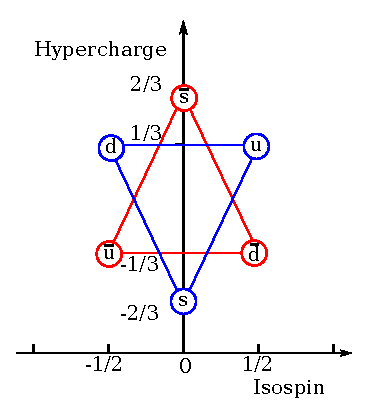
\includegraphics[width=0.3\textwidth]{theory/figures/threequarks}}\\
	\subfigure[]{
  	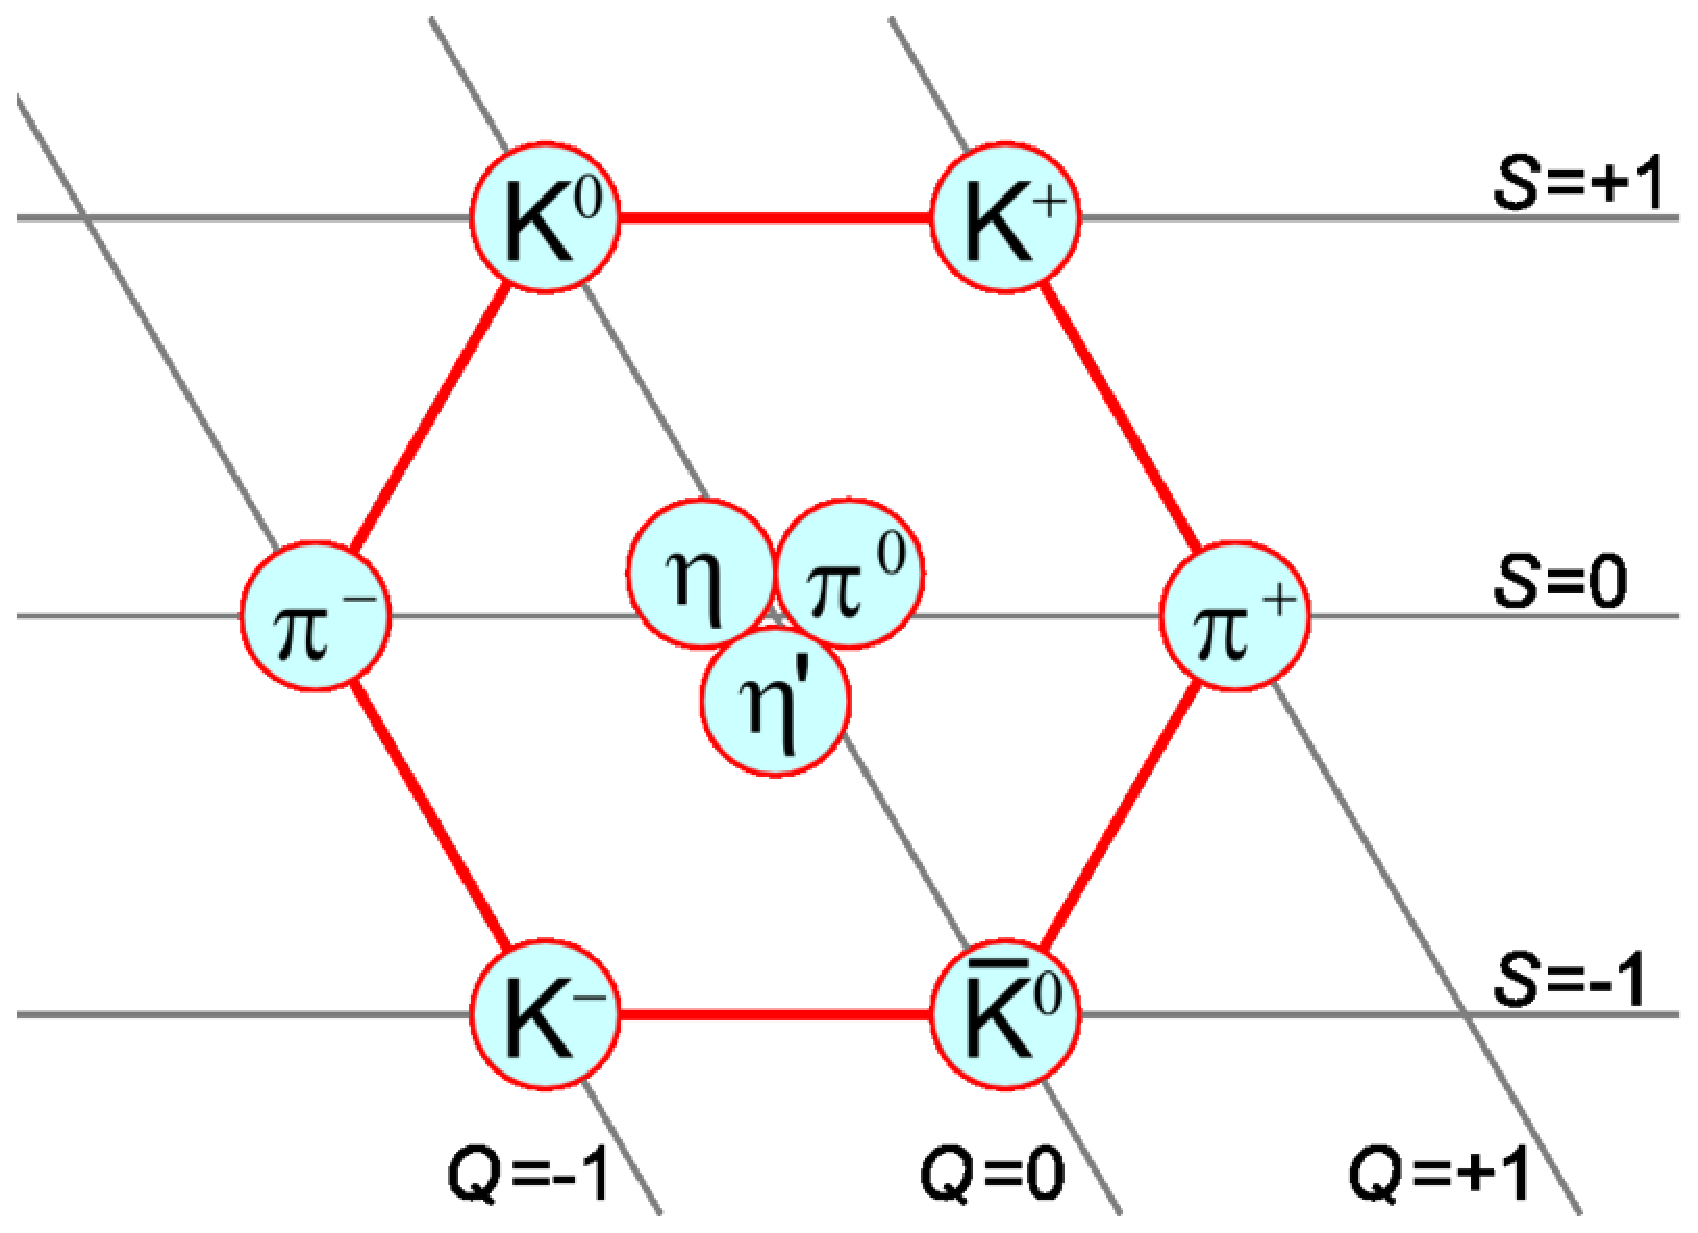
\includegraphics[width=0.37\textwidth]{theory/figures/mesons}}
	\subfigure[]{
  	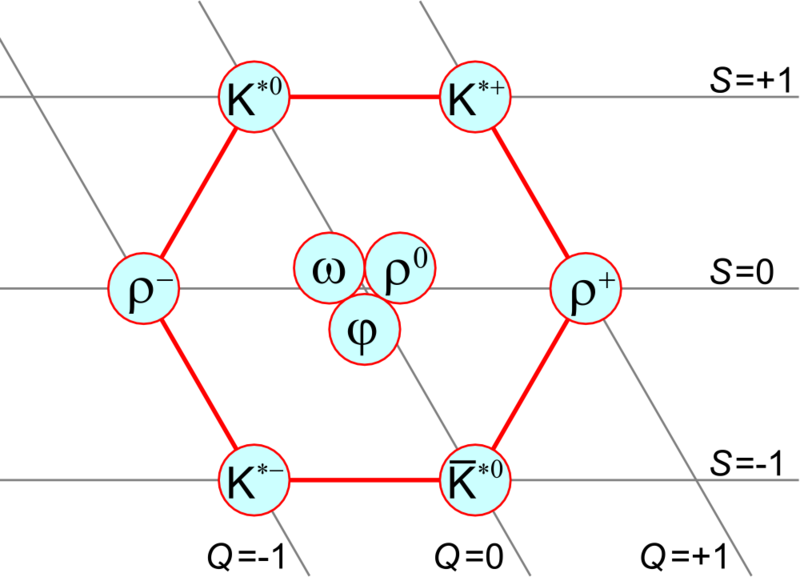
\includegraphics[width=0.37\textwidth]{theory/figures/mesons1}}
	\subfigure[]{
  	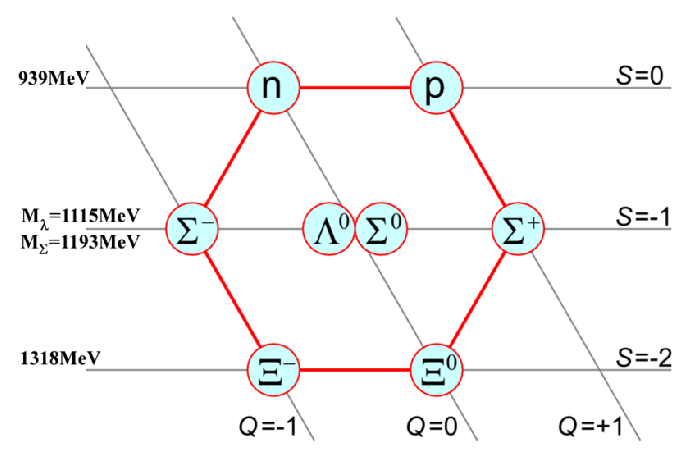
\includegraphics[width=0.4\textwidth]{theory/figures/Baryon_octet_w_mass}}
	\subfigure[]{
 	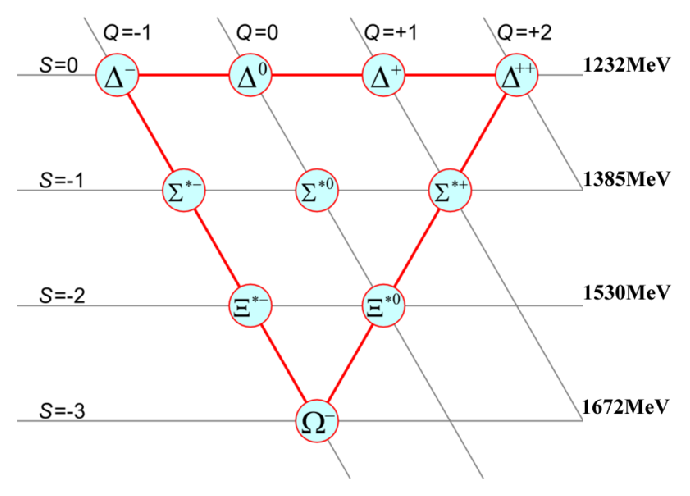
\includegraphics[width=0.4\textwidth]{theory/figures/Baryon_decuplet_w_mass}}
	\caption{Gell-Mann's \textit{Eightfold Way} (proposed also independently 
          by Yuval Ne'eman) identifies three fundamental components (a) 
          and classifies through their electric charge $q$ and strangeness $s$:
          a spin-0 meson octet (b), a spin-1 meson octet (c), 
          a spin-1/2 baryon octet (d) and a spin-3/2 baryon decuplet (e).
          It is now understood that this structure is a 
          consequence of a flavour symmetry.\label{fig:eightfold}}
\end{center}\end{figure}

It was the beginning of the {\it quark model}, a theory that had to 
wait for multiple experimental evidence before being accepted,
nevertheless it successfully predicted a new particle, the strangeness $s$=-3 
particle $\Omega^{-}$ of the spin-3/2 baryon decuplet of Figure~\ref{fig:eightfold},
discovered in 1964 at Brookhaven~\cite{PhysRevLett.12.204}. 
Even when in 1968 deep inelastic experiments at the Stanford 
Linear Accelerator Center (SLAC) found out evidence for a 
substructure in protons~\cite{PhysRevLett.23.930,PhysRevLett.23.935}, 
physicists were reluctant to accept 
these point-like objects to be the quarks. Richard Feynman called 
them \textit{partons}, the term now used to refer to quarks 
and antiquarks as well as gluons.

However, back then there was a tougher problem tormenting theoretical physicists. 
Quantum field theory was apparently unsuitable for the description 
of the dynamics of particles interactions, since divergences appeared in the 
high-energy domain. In 1954 C. N. Yang and R. Mills proposed a new gauge 
theory~\cite{PhysRev.96.191} based on the principle of {\it local gauge invariance},
i.e. the property of space-time regions of not being affected 
by a symmetry transformation performed 
locally in a different region. With the addition of a scalar 
field proposed by Peter Higgs, 
Fran\c{c}ois Englert and Robert 
Brout~\cite{PhysRevLett.13.321,PhysRevLett.13.508} and the implied 
modification of the vacuum structure, the Yang-Mills theory 
became a very accurate description of weak force interactions. 
Such unified model was consistently proposed, independently, in the 1960s by  
%Abdus Salam, Sheldon Glashow and Steven Weinberg~\cite{Glashow1961579,PhysRevLett.19.1264}, 
S. Glashow, S. Weinberg and A. Salam~\cite{Glashow1961579,PhysRevLett.19.1264,Salam},
but it suffered from a problem: 
as it was a perturbative theory, equations 
had to be expanded in a power series to be calculated but only the leading order 
term did not show ultraviolet divergences\footnote{Divergences in computations
are classified according to the energy scale at which they appear. Following
the Planck relation $E=h\nu$ and the relation between the wave lenght and
the frequency of radiation $\lambda\nu = c$, in natural units 
($\hbar=c=1$) energies of the order of 1~\tev\ 
or more lie in the ultraviolet (UV) range: $\lambda({\rm UV})\sim 10^{-9}$~m.
Divergencies appearing at the energy scale of 1~\gev\ or less are in the 
infrared (IR) range: $\lambda({\rm IR})\sim 10^{-6}$~m.}.

By the first years of the 1970s Gerard't Hooft demonstrated in his
PhD thesis under the supervision of  Martinus Veltman the
renormalization for the theory~\cite{tHooft1971173,Hooft1971167}, 
with the result that divergences could be 
cancelled and physical observables obtained with precision higher than the 
leading order. 
The concept of \textit{renormalization group} was introduced and 
Yang-Mills theories were found to have a $\beta$-function (a function 
typical of gauge theories) generally negative which describes
the behavior of the running coupling.
 This was the discovery 
of \textit{asymptotic freedom}, a property that made Yang-Mills theory 
suitable also to describe strong interactions and that matched properly 
with the experimental effect referred to as \textit{Bjorken scaling}\footnote{At 
SLAC it was observed during deep inelastic scattering experiments that 
strong interactions show a decrease of strenght at short distances (i.e. 
high momentum transfer) together with a scaling behaviour. A property is 
said to ``scale'' when it depends only by dimensionless kinematic quantities, 
such as a scattering angle or the ratio of the energy to a momentum transfer.}. 

At the same time, the three-quark model by Gell-Mann and Zweig was about to 
be expanded. In 1963 Nicola Cabibbo proposed the mixing of up, down and 
strange quarks~\cite{PhysRevLett.10.531} 
in order to explain the non-conservation of quark flavour 
in weak interactions as $\Lambda \rightarrow p^{+}\pi^{-}$ with $\Delta S$=1 
and the empirical law $\Delta S = \Delta Q$ for strangeness changing processes. 
In 1970 Glashow, Iliopoulos and Maiani (GIM) predicted a fourth quark~\cite{PhysRevD.2.1285}, 
the charm, to account for the non-observation of strangeness-changing-neutral-current 
processes. Thus, the quark mixing between the two families
of quarks ($u$, $d$) and ($c$, $s$) could be described with a $2\times 2$ 
matrix, parameterized by the Cabibbo angle $\theta_{C}$ and referred to as
 the Cabibbo-GIM matrix:
\begin{equation}\label{CabibboGIM}
V_{c} = {\setlength\arraycolsep{6pt}
\left( \begin{array}{cc}
\cos\theta_{C} & \sin\theta_{C}\\
-\sin\theta_{C}& \cos\theta_{C}
\end{array}
\right)} \quad .
\end{equation}
Furthermore, after the observation of events violating the Charge-Parity (CP) 
symmetry~\cite{PhysRevLett.13.286}, Makoto Kobayashi and 
Toshihide Maskawa supposed the 
existence of two more quarks, the bottom and the top, thus increasing 
the number of quark flavours to six~\cite{Kobayashi:1973fv}. 
This allowed the introduction in 
the extended (now $3\times 3$) mixing matrix (the Cabibbo-Kobayashi-Maskawa, or CKM matrix) 
of, besides three angles, a complex phase that is responsible of CP violation. 
All this conjectures found an important confirmation in November 1974, a date
later known as ``the November Revolution'', probably because it set the 
beginning of a real trust in the quark theory. 
Almost simultaneously at SLAC and at Brookhaven the charm quark was discovered 
in the bound state $c\bar c$, called $J$ meson by the Brookhaven team and 
$\psi$ by the SLAC one, so that in the end it was named $J/\psi$~\cite{PhysRevLett.33.1404,PhysRevLett.33.1406}. 
Not much later, the bottom quark was observed in 1977 at 
Fermilab~\cite{PhysRevLett.39.252}, 
raising the level of confidence in the top quark existence and in the six flavours theory.

The discovery of the tau lepton in 1975~\cite{PhysRevLett.35.1489} and of the 
$W$ and $Z$ bosons in 1983~\cite{Arnison1983103,Banner1983476} finally set the scene for 
the Standard Model (SM) of particle physics. Table~\ref{tab:SM} 
shows the fundamental particles composing the SM: three generations of 
fermions, each of them having a corresponding 
antiparticle, the three forces (three Yang-Mills fields) with 
their vector bosons, and the Higgs boson whose field interaction with
particles results in the lagrangian mass terms. A great achievement of the SM was 
the unification of electromagnetic and weak theories in the Electroweak 
Theory by Salam, Glashow and Weinberg. In fact, since at a scale of about 
100~GeV the coupling constants converge, it is possible to describe them 
within the same mathematical model. Quantum ChromoDynamics (QCD) instead 
describes the strong interaction in terms of the threefold color charge 
and up to now is not known if also the strong coupling constant can become 
equal to the others at some high energy scale. However, a unified theory is 
strongly desired, as will be stressed in Section~\ref{sec:THquest}.
\begin{table}[htb]\centering\begin{tabular}{c x{.15\textwidth} x{.15\textwidth} x{.15\textwidth} x{.15\textwidth}}\toprule
           & \multicolumn{2}{c}{Leptons}&\multicolumn{2}{c}{Quarks} \\ 
Fermion    & \multicolumn{2}{c}{spin 1/2}& \multicolumn{2}{c}{spin 1/2}\\
generation & $q=-1$ & $q=0$ &$q=2/3$ &$q=-1/3$ \\ \midrule
I & $e^{-}$ & $\nu_{e}$ & $u$ & $d$ \\
II & $\mu^{-}$ & $\nu_{\mu}$ & $c$ & $s$ \\
III & $\tau^{-}$ & $\nu_{\tau}$ & $t$ & $b$ \\\bottomrule\toprule
Force & Electromagnetic &\multicolumn{2}{c}{Weak}& Strong\\\midrule
Carrier boson & $\gamma$ & $W^{\pm}$ &$Z$ & $g$\\
spin & 1 & 1 &  1 & 1 \\
$q$ & 0 & $\pm$1 & 0 & 0\\\bottomrule\toprule
 \multicolumn{2}{c}{Higgs boson $H$}& \multicolumn{3}{c}{$q=0$, spin=0} \\
\bottomrule
\end{tabular}\caption{Elementary particles and forces of the SM.}\label{tab:SM} \end{table}


\section{Building the Standard Model}\label{sec:THlagr}

The Standard Model (SM) is a gauge theory invariant under the symmetry 
transformation $SU(3)_{C} \otimes SU(2)_{L} \otimes U(1)_{Y}$. The
three terms of the product of groups are the matrix representations
of the fundamental symmetries acting on the forces of Nature ({\it quantum fields})
governing the interactions of particles: 
$SU(3)_{C}$ is the {\it color} unbroken 
symmetry %containing the color triplets %, described by Quantum ChromoDynamics (QCD) 
 acting on the gluon field $G_a$; 
$SU(2)_{L} \otimes U(1)_{Y}$ is the unified {\it electroweak} broken 
symmetry, %described by Quantum ElectroDynamics (QED), 
with the symmetry $SU(2)_{L}$
%containing the left-handed weak isospin doublets 
acting on the vector boson fields $W_{1,2,3}$ and on the scalar Higgs field $\phi$,
and the symmetry $U(1)_{Y}$ %containing the right-handed isospin singlets.
acting on the vector boson field $B$ and on the scalar Higgs field $\phi$.

The quantum number $C$, the color charge, is carried only by
quarks, antiquarks and gluons 
and comes in three different values labelled ``red'', ``gree'', ``blue''.
The quantum number $I$, the weak isospin, differentiates between left-handed
($I=1/2$) and right-handed ($I=0$) fermions, with the latter 
not undergoing charged-current weak interactions.
 %The quantum number $L$, the flavor charge, is carried by fermions as
 %{\it lepton number} for leptons and as {\it baryon number} for quarks.
The quantum number $Y$, the hypercharge, is defined as $Y=2(Q-I_3)$, 
where $Q$ is the electric charge and $I_3$ the third componend of the isospin,
which is $I_3=+1/2$ for up-type quarks and negatively charged leptons, and
 $I_3=-1/2$ for down-type quarks and neutrinos (and {\it vice-versa} for the antiparticles).

%These quantum numbers are the generators for the

Gravity is not (yet) included in the model, and even though
this is a limitation of the SM that is desirable to be fixed in a 
Grand Unified Theory (GUT), 
its action on particles is about $10^{38}$ 
times weaker than
the EM strength
%its action on particles is of many order of magnitudes lower than the others' 
and is, therefore, negligible at the
fundamental components scale.


\subsection{Building the electroweak lagrangian}\label{sec:ewlagr}

The Lagrangian of the SM is built by {\it gauging} the symmetries in 
order to obtain invariance under their transformations.
Fermions are spin-1/2 particles that can be represented as spinors.
Using $\psi_{L}$ and 
$\psi_{R}$ to denote the left-handed and right-handed fermion fields 
respectively, 
the bare electroweak Lagrangian of the SM (considering 
for simplicity only leptons) is made of two terms:
\begin{equation}\label{eq:bareLagSM}
\mathcal{L}_{0} = \mathcal{L}_{lept}+ \mathcal{L}_{gauge}
\end{equation}
that are 
\begin{align}
&\left \{ \begin{array}{cl}
\mathcal{L}_{lept} &=\;\;  \bar\psi_{L}i\slashed{D}_{L}\psi_{L} + \bar\psi_{R}i\slashed{D}_{R}\psi_{R}\\
D_{L}^{\mu} &=\;\;  \partial^{\mu} + ig\dfrac{\bar{\sigma}\cdot\bar{W}^{\mu}}{2} + i\dfrac{g'}{2}Y_{L}B^{\mu}\\
D_{R}^{\mu} &=\;\;  \partial^{\mu} + i\dfrac{g'}{2}Y_{R}B^{\mu}
\end{array} \right. ,\label{eq:lagLep} \\
&\left \{ \begin{array}{cl}
\mathcal{L}_{gauge}  &=\;\;  -\frac{1}{4}W_{\mu\nu}^{l}W^{\mu\nu\, l}  -\frac{1}{4}B_{\mu\nu}B^{\mu\nu}\\
B_{\mu\nu} &=\;\;  \partial_{\mu}B_{\nu} - \partial_{\nu}B_{\mu}\\
W_{\mu\nu}^{l} &=\;\;  \partial_{\mu}W_{\nu}^{l} - \partial_{\nu}W_{\mu}^{l} - g\varepsilon^{jkl}W_{\mu}^{j}W_{\nu}^{k}
\end{array} \right. .\label{eq:lagGauge}
\end{align}
The gauge invariance is obtained through the definition of the
covariant derivatives $\slashed{D} = \gamma_{\mu}D^{\mu}$, 
which are different for the left- and
right-handed components of the field.
The chirality of the electroweak interactions does not find 
a theoretical motivation, but $SU(2)_{L} \otimes U(1)_{Y}$ transformations 
do make distinction between left and right helicity of the spinors.
Introducing the Weyl representation of the $\gamma$ matrices
\begin{equation}
\gamma^{0} = \left(\begin{array}{cc} 0 & 1 \\ 1 & 0 \\ \end{array}\right), \quad
\gamma^{i} = \left(\begin{array}{cc} 0 & \sigma^{i} \\ -\sigma^{i} & 0 \\ \end{array}\right) \quad \textnormal{and} \quad
\gamma^{5} = \left(\begin{array}{cc} -1 & 0 \\ 0 & 1 \\ \end{array}\right) \quad ,
\end{equation}
where $\sigma_{i}$ are the Pauli matrices, the left- and right-handed spinors transform as:
\begin{align}
&\left \{ \begin{array}{ll}
\psi_{L} = \frac{1}{2}(1 - \gamma_{5})\phi &\rightarrow \; \psi_{L}' = e^{iY\beta(x) + i\bar{\sigma}\bar{\alpha}(x)}\psi_{L} \\
\psi_{R} = \frac{1}{2}(1 + \gamma_{5})\phi &\rightarrow \; \psi_{R}' = e^{iY\beta(x)}\psi_{R}
\end{array} \right. .
\label{eq:chiral}
\end{align}

Equation~\ref{eq:lagLep} is the ``free matter'' Lagrangian 
describing the transformation under the symmetry $SU(2)_{L}$ of weak isospin
with coupling constant $g$, three boson fields $W^{l}_{\mu\nu}$ and
their weak generators $\bar{\sigma}$\footnote{These are the Pauli matrices: 
$$
\sigma_{1} = \left(\begin{array}{cc} 0 & 1 \\ 1 & 0 \\ \end{array}\right), \quad
\sigma_{2} = \left(\begin{array}{cc} 0 & -i \\ i & 0 \\ \end{array}\right), \quad
\sigma_{3} = \left(\begin{array}{cc} 1 & 0 \\ 0 & -1 \\ \end{array}\right).
$$}, and under the symmetry
$U(1)_{Y}$ of hypercharge with coupling constant $g'/2$,
the boson field $B_{\mu\nu}$ and its hypercharge generator $Y$.
Equation~\ref{eq:lagGauge} is the Lagrangian for the vector bosons 
dynamics with self-interactions, including trilinear and quadrilinear terms. 



The Lagrangian \ref{eq:bareLagSM} is invariant under group 
$SU(2)_{L} \otimes U(1)_{Y}$ transformation, but has the 
problem of leaving fermions massless. Thus a scalar 
Lagrangian with a quartic auto-interaction is introduced:
\begin{equation}\label{eq:lagScalar}
\left \{ \begin{array}{cl}
\mathcal{L}_{\phi} &=\;\;  (D_{\phi}^{\mu} \phi)^{\dag}(D_{\phi\,\mu} \phi) - V(\phi^{\dag}\phi)\\
V &=\;\; \mu^{2}\phi^{\dag}\phi + \lambda(\phi^{\dag}\phi)^{2}\\
D_{\phi}^{\mu} &=\;\; \partial^{\mu} + ig\dfrac{\bar{\sigma}\cdot\bar{W}^{\mu}}{2} + i\dfrac{g'}{2}Y_{\phi}B^{\mu}
\end{array}\right. ,
\end{equation}
where $\phi$ is an Higgs doublet, accounting for four 
degrees of freedom needed to give mass to three vector
bosons (the neutral $Z$ boson and the two $W^{\pm}$ bosons)
and to a scalar Higgs boson:
\begin{equation}\label{eq:higgsDoub}
\phi = \begin{pmatrix} \varphi^{+}\\\varphi^{0}
\end{pmatrix} =
\dfrac{1}{\sqrt{2}} 
\begin{pmatrix} \varphi_{1}+i\varphi_{2}\\ \varphi_{3}+i\varphi_{4}\end{pmatrix},
\end{equation}
since, according to the Nambu-Goldstone theorem~\cite{PhysRev.127.965},
for every broken continuous symmetry a massless and spinless particle, 
the {\it Goldstone boson}, arises, which can be ``eaten'' by a gauge 
boson which will in this way acquire mass.
%become massive and their new, longitudinal polarization is provided by the Goldstone boson.


%Three terms, $\varphi^{+}$, $\varphi^{-}$ and $(\varphi^{0}-\bar\varphi^{0})/\sqrt{2}$, give mass to the three massive vector bosons $W^{\pm}$ and $Z$, leaving a massive Higgs scalar boson $(\varphi^{0}+\bar\varphi^{0})/\sqrt{2}$. 
The potential $V(\phi)$ depends on two parameters, $\mu^2$ and $\lambda$. 
The case $\lambda<0$ is unphysical, leading to no stable minima. For 
$\lambda>0$, two cases arise: $\mu^2>0$ and $\mu^2<0$. In the first case
(see Figure~\ref{fig:higgs1}) there is a single solution to the minimization
which corresponds to $|\phi|=0$ and gives as vacuum expectation value
$\bra{0}\phi \ket{0} = 0$. In the second case (see Figure~\ref{fig:higgs2}) 
the potential has a non-vanishing vacuum expectation value 
$\bra{0}\phi \ket{0} = v$ and %the symmetry is spontaneously broken, the minimum not being unique anymore.
there is no unique minimum. The fundamental vacuum 
state is no more invariant under $SU(2)_{L} \otimes U(1)_{Y}$, 
meaning that these two symmetries are now 
broken\footnote{Instead, the symmetry $U(1)_{EM} \subset SU(2)_{L} \otimes U(1)_{Y}$ 
is not broken. This means that vacuum is electrically-neutral while 
it has non-zero isospin and hypercharge charges.}: 
this is the Spontaneous Symmetry Breaking (SSB) mechanism. 
The vacuum state is chosen as:
\begin{figure}[h!tb]\begin{center}
	\subfigure[]{\label{fig:higgs1}
  	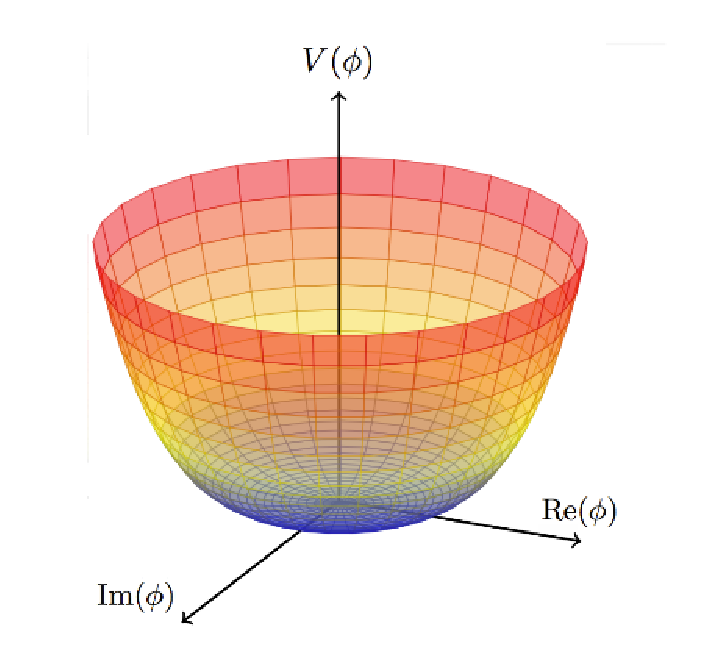
\includegraphics[width=0.45\textwidth]{theory/figures/higgs1.eps}}
	\subfigure[]{\label{fig:higgs2}
  	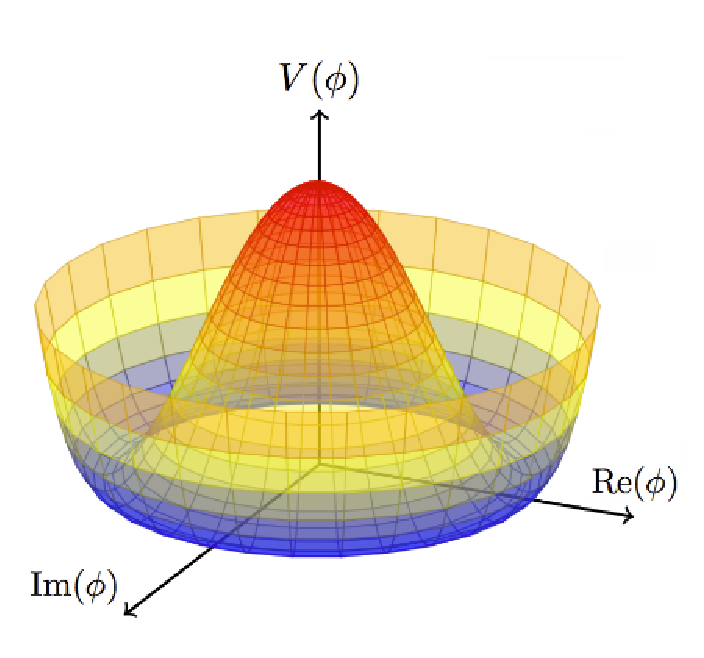
\includegraphics[width=0.45\textwidth]{theory/figures/higgs2.eps}}
	\caption{Vacuum pontential for $\lambda>0$ and (a) $\mu^2>0$ or
          (b) $\mu^2<0$, with the typical shape of a mexican hat~\cite{Michael:1569839}.}
\end{center}\end{figure}

\begin{equation}\label{eq:vacuum}
\phi_{0} = \begin{pmatrix} 0 \\ v/\sqrt{2}
\end{pmatrix}
\end{equation}
where $v = \sqrt{-\mu^{2}/\lambda}$ is 
the vacuum expectation value. Finally, since
only the vector bosons got their mass up to now
by directly ``eating'' the Goldston bosons
(while the fact that $U(1)_{Q}$ is unbroken 
causes the photon to remain massless),
the only thing left to do is to introduce 
the scalar-fermion interaction in order to give
mass to the fermions. This is done defining
an explicit Yukawa coupling $G_{lept}$ that gives:
\begin{equation}\label{eq:lagYukawa}
\mathcal{L}_{Yukawa} = -G_{lept}\big[\bar\psi_{R}(\phi^{\dag}\psi_{L}) + (\bar\psi_{L}\phi)\psi_{R}\big] .
\end{equation}Thus the complete electroweak Lagrangian of the SM, that can be generalized also to quarks (see Table \ref{tab:isospin}), is\begin{equation}\label{eq:lagSM}
\mathcal{L}= \mathcal{L}_{lept} +\mathcal{L}_{gauge} +\mathcal{L}_{\phi} +\mathcal{L}_{Yukawa}.
\end{equation}

\begin{table}[htb]\centering\begin{tabular}{cccc}\toprule
\multicolumn{4}{c}{Weak isospin left-handed doublets \bfseries $\psi_{L}$} \\ \midrule \\ 
$\begin{pmatrix} \nu_{e_{L}} \\ e_{L} \end{pmatrix}$ & $\begin{pmatrix} \nu_{\mu_{L}} \\ \mu_{L} \end{pmatrix}$ &$\begin{pmatrix} \nu_{\tau_{L}} \\ \tau_{L} \end{pmatrix}$ & \bfseries Leptons \\ \\ 
$\begin{pmatrix} u_{L} \\ d'_{L} \end{pmatrix}$ & $\begin{pmatrix} c_{L} \\ s'_{L} \end{pmatrix}$ &$\begin{pmatrix} t_{L} \\ b'_{L} \end{pmatrix}$ & \bfseries Quarks \\
 \\ \bottomrule\\ \toprule
\multicolumn{4}{c}{Weak isospin right-handed singlets \bfseries $\psi_{R}$} \\ \midrule \\ 
$ e_{R} $ & $ \mu_{R}$ &$\tau_{R}$ & \bfseries Leptons \\ \\ 
$u_{R}$ , $d'_{R} $ & $c_{R}$ , $s'_{R} $ &$ t_{R}$ , $b'_{R}$ & \bfseries Quarks \\
 \\ \bottomrule
\end{tabular}\caption{Weak isospin multiplets. $q'$ refers to the flavour eigenstate that correspond to the mass eigenstate transformed with the CKM matrix.}\label{tab:isospin} \end{table}

An important consequence of the introduction of the scalar Higgs 
field and the consequent spontaneous symmetry breaking
is the mixing of the vector bosons $B_{\mu}$ and $W^{1,2,3}_{\mu}$ 
to give the photon $A_{\mu}$, the two $W^{\pm}_{\mu}$ and 
the $Z_{\mu}$ bosons:
%\begin{equation}\label{eq:AZ}
%\left \{ \begin{array}{ll}
%A^{\mu} = \cos\theta_{W}B^{\mu} + \sin\theta_{W}W_{3}^{\mu}\\
%Z^{\mu} = -\sin\theta_{W}B^{\mu} + \cos\theta_{W}W_{3}^{\mu}\end{array}\right. ,
%\end{equation}
\begin{align}
  W_{\mu}^{\pm} & = \frac{1}{\sqrt{2}}\left(W_{\mu}^{1}\mp i W_{\mu}^{2}\right), \label{eq:Wpm} \\
  \left(
  \begin{array}{c}
  A_{\mu} \\ Z_{\mu}
  \end{array}
  \right)
  & =
  \left(
  \begin{array}{cc}
  \cos\theta_{W} & \sin\theta_{W} \\
  -\sin\theta_{W} & \cos\theta_{W}
  \end{array}
  \right)
  \left(
  \begin{array}{c}
  B_{\mu} \\ W_{\mu}^{3}
  \end{array}
  \right) , \label{eq:AZ}
\end{align}
where the Weinberg angle $\theta_{W}$ is defined through\begin{equation}\label{eq:weinb}
\left \{ \begin{array}{ll}
\dfrac{g}{\sqrt{(g')^{2}+g^{2}}} = \cos\theta_{W} \\
\dfrac{g'}{\sqrt{(g')^{2}+g^{2}}} = \sin\theta_{W} \end{array}\right. .
\end{equation} 
The mass terms that arise from the Higgs mechanisms are finally:
\begin{align}
  m_W & =  \dfrac{1}{2}vg \quad \quad \quad & \textnormal{for} & \quad \quad \quad
  & W^{\pm}_{\mu} & = \dfrac{1}{\sqrt{2}}\left(W^{1}_{\mu} \mp i W^{2}_{\mu}\right), \quad & \\
  m_Z & =  \dfrac{1}{2}v\sqrt{g^{2}+{g'}^{2}}
  \quad \quad \quad & \textnormal{for} & \quad \quad \quad
  & Z_{\mu} & = \dfrac{gW^{3}_{\mu} - g'B_{\mu}}{\sqrt{g^{2}+{g'}^{2}}}, \quad & \\
  m_{\gamma} & =  0
  \quad \quad \quad & \textnormal{for} & \quad \quad \quad
  & A_{\mu} & = \dfrac{g'W^{3}_{\mu} + gB_{\mu}}{\sqrt{g^{2}+{g'}^{2}}}, \quad & 
\end{align}
$m_l = v G_{lept}/\sqrt{2}$ for leptons and $m_H = v\sqrt{2\lambda}$ for the Higgs boson. 
The experimental values for the masses of Standard Model particles
are listed in Table \ref{tab:mass}.


\begin{table}[htb]\centering

%\begin{minipage}{.2\textwidth}
    \begin{tabular}{cccc}\toprule
      Spin-$1$ & \multirow{2}{*}{mass} & Spin-0 & \multirow{2}{*}{mass}\\
      gauge bosons & & scalar boson & \\\midrule
    $\gamma$      & 0  & \multirow{4}{*}{$H$} & \multirow{4}{*}{$\sim 125~\gev$}                        \\
    $g$           & 0  & &                        \\
    $W^{\pm}$ & $ 80.385 \pm 0.015 \gev$ & &\\
    $Z$       & $ 91.188 \pm 0.002 \gev$ & &\\\bottomrule
    \end{tabular}

%\end{minipage}\begin{minipage}{.7\textwidth}
    \begin{tabular}{ccccccc}\toprule
      Spin-$\tfrac{1}{2}$ &  \multicolumn{2}{c}{\multirow{2}{*}{I generation}}
      &  \multicolumn{2}{c}{\multirow{2}{*}{II generation}}
      &  \multicolumn{2}{c}{\multirow{2}{*}{III generation}}\\
      fermions & & & & & \\\midrule
    \multirow{2}{*}{leptons} &
    $\nu_{e}$   & \small{$\sim 0$} &  
    $\nu_{\mu}$ & \small{$\sim 0$} &  
    $\nu_{\tau}$ & \small{$\sim 0$} \\
    &
    e            & \small{$511\kev$}   &  
    $\mu$ & \small{$105.7\mev$} &  
    $\tau$     & \small{$1.777\gev$} \\
    \multirow{2}{*}{quarks} &
    u & \small{$1.7-3.1\mev$}         &  
    c & \small{$1.29^{+0.05}_{-0.11}\gev$}  &  
    t & \small{$173.2^{+0.87}_{-0.87}\gev$}\\ %$172.9^{+1.1}_{-1.1}\gev$} \\
    &
    d & \small{$4.1-5.7\mev$} &  
    s & \small{$100^{+30}_{-20}\mev$} &  
    b & \small{$4.19^{+0.18}_{-0.06}\gev$} \\\bottomrule
    \end{tabular}
%\end{minipage}
  \caption{Experimental values for the elementary particles of the Standard Model.\label{tab:mass}}

\end{table}


\subsection{Adding the strong interaction}\label{sec:qcdlagr}

Adding the color transformations $SU(3)_{C}$, the Standard Model is
finally described by the symmetry group 
$SU(3)_{C}\otimes SU(2)_{L}\otimes U(1)_{Y}$.
In the same way electromagnetic interactions are 
described by Quantum ElectroDynamics (QED), 
strong interactions are described by Quantum ChromoDynamics (QCD~\cite{Ecker}).
However, while the photon does not carry electric charge,
the gluon does carry color charge (in particular it exists in
eight states, being a color octet) and can, therefore, self-interact.

The QCD lagrangian only involves quarks and gluons, and reads:
\begin{equation}
\left \{ \begin{array}{cl}
\mathcal{L}_{QCD} &=\;\; \sum\limits_{f=1}^{6}\bar{q}(i\gamma^\mu D_\mu - m_q)q 
                    -\frac{1}{4}F^{\mu\nu}_{a}F^{a}_{\mu\nu}\\
 D_\mu &=\;\; \partial_\mu + ig_sG_\mu^a T^a\\
  F^{a}_{\mu\nu} &=\;\;  \partial_\mu G_\nu^a - \partial_\nu G_\mu^a - 
                    g_sf^{a}_{\ bc}G^b_\mu G^c_\nu
\end{array} \right.
\end{equation}
where $q$ is the quark field and $m_q$ is the quark mass, summed over 
the six flavors ($f$) of quarks, and $a$ runs over the eight degrees of 
freedom of the gluon field, $T^a$ being the generators
of the $SU(3)_C$ group. The field tensor $F^{a}_{\mu\nu}$ 
is derived from the gluon field $G_\mu^a$ and 
its third term describes the gluon self-interaction, with
$f^a_{\ bc}$ being the structure constants
of the $SU(3)_{C}$ group. 
%non-abelian nature  of the QCD, and it describes the
The strong coupling constant $\alpha_s$ is defined
as  $\alpha_s=g_s/4\pi$ and its values, large at
low energies (i.e. large distances), and small at high 
energies (i.e. short distances), determine the 
peculiar property called {\it asymptotic freedom} which
explains the confinement of the quarks inside the hadrons
(see Figure~\ref{fig:alpha_s}). Indeed, at
small distances $\alpha_s$ is so small that
the strong interaction can be treated perturbatively
and quarks and gluons described as free particles.
On the other hand, a quark cannot be found
isolated since at large distances the field strength
will increase enough to create new quarks 
from the vacuum and colorless hadrons will be formed.

\begin{figure}[tbph]
\begin{center}
\subfigure{
  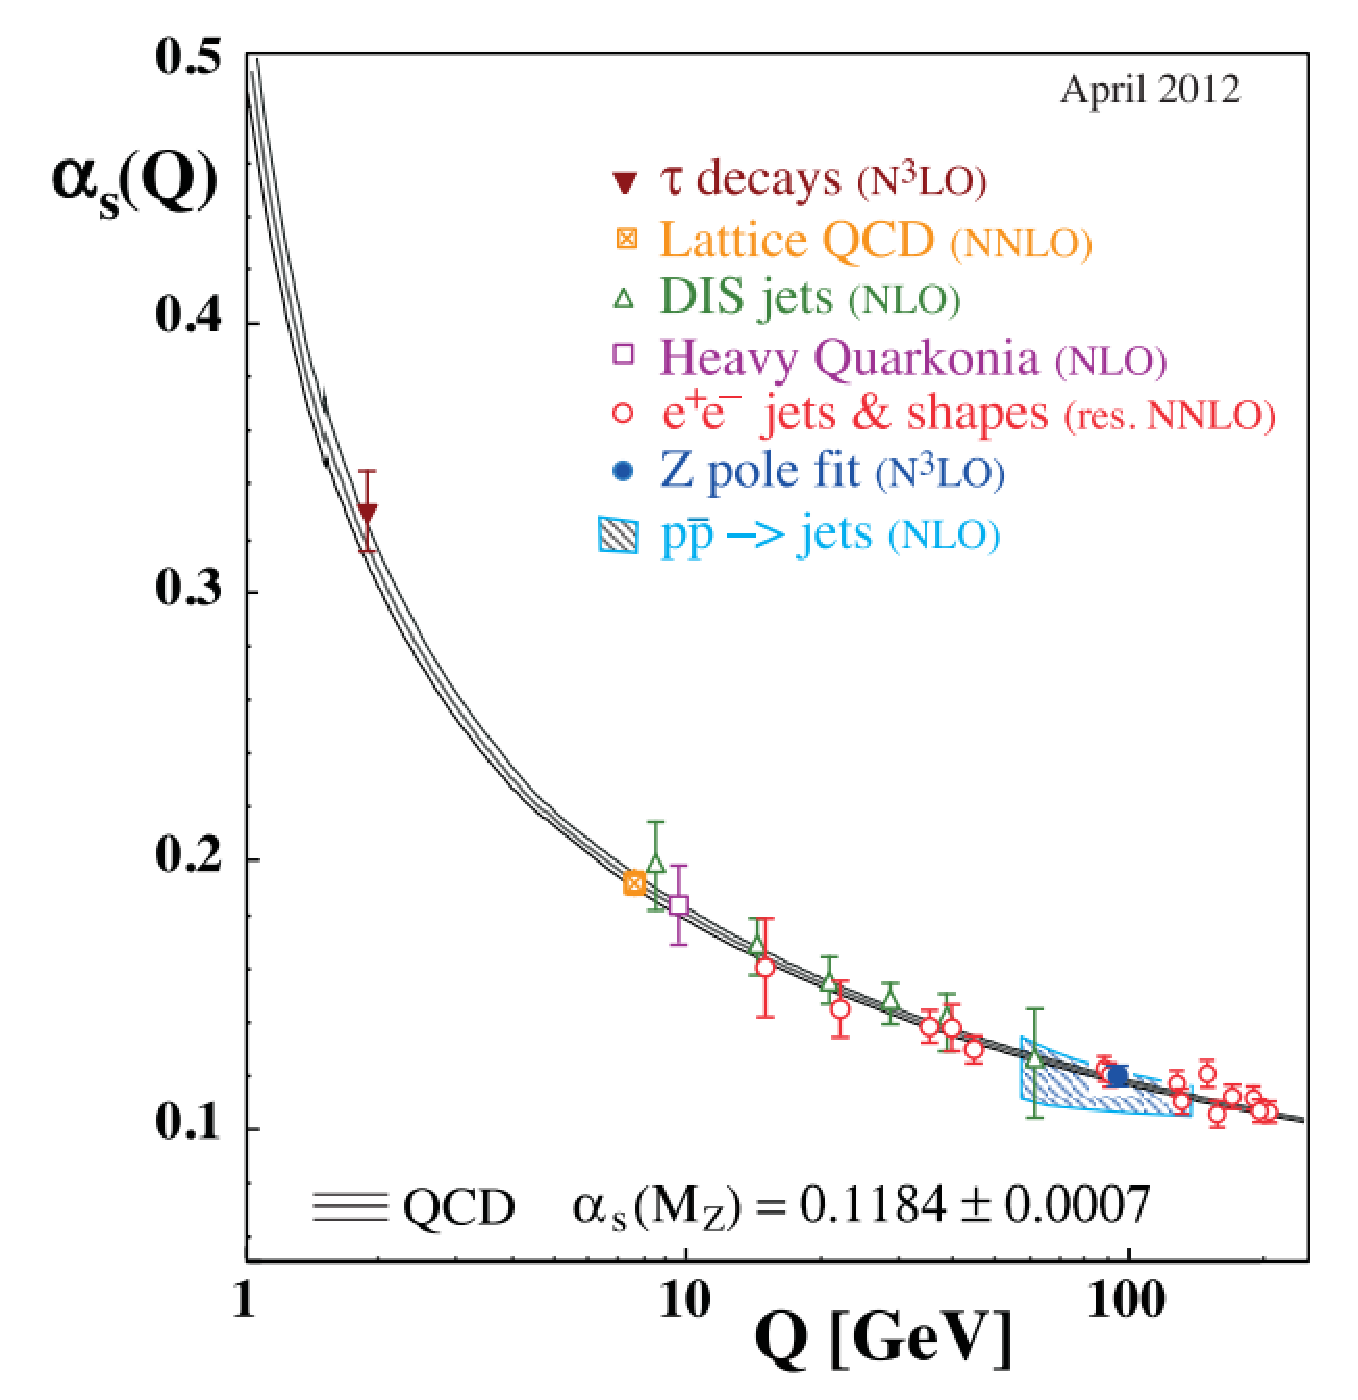
\includegraphics[width=0.5\textwidth]{theory/figures/asq-2012.eps}
}
\caption{Running of the strong coupling $\alpha_s$ with the energy scale $Q$,
proven from different measurements~\cite{alpha_s}.}
\label{fig:alpha_s}
\end{center}
\end{figure}

As an example of how quarks behave in hadrons,
protons are composed of two {\it valence} up quarks
and one {\it valence} down quark. The quarks continuosly
exchange gluons, which create in turn quark-antiquark pairs,
resulting in what is referred to as a ``sea'' 
of quarks and gluons. 
%randomly created and annihilated in vacuum fluctuations. 
As the sum of the rest masses of the valence quarks contributes 
only to about 1\% of the total nucleon
mass, what accounts for the missing 99\% is the
binding energy of gluons and sea quarks.
Further details on QCD will be given in Section~\ref{sec:MCphenomenology},
where the phenomenology of proton-proton collision
is discussed.



\subsection{Experimental success of the Standard Model}\label{sec:THsuccess}

Even if the SM was somehow born to be merely a stepping stone, 
it consolidated through the years, standing all experimental tests 
sometimes with a precision greater than 0.1\%. Experiments carried 
out at the Large Electron-Positron (LEP) collider at CERN, 
thanks to the clean signals given by $e^{+}e^{-}$ collision events, 
allowed to obtain very high precision measurements of the SM parameters
(see Figure~\ref{fig:smparam}). %for a summary of the measurements, with their errors, of the free parameters of the SM).
\begin{figure}[htb]\begin{center}
	\subfigure[]{\label{fig:smparam}
  	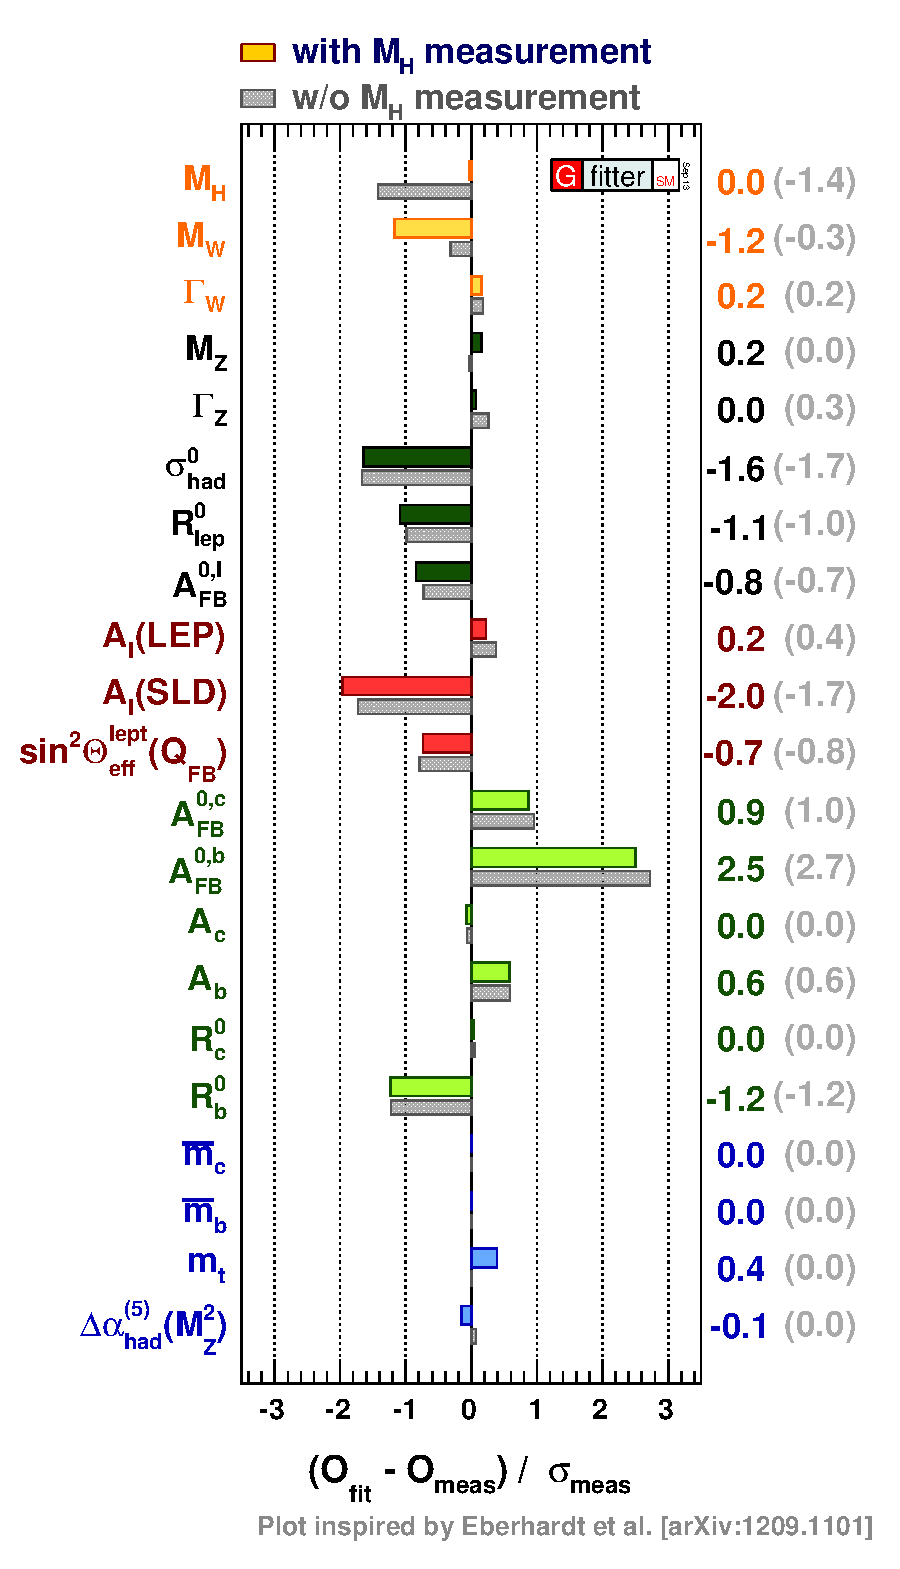
\includegraphics[width=0.35\textwidth]{theory/figures/fitSM_new.eps}}%cernlep5_5-04}}	
	\subfigure[]{\label{fig:WtopMass}
  	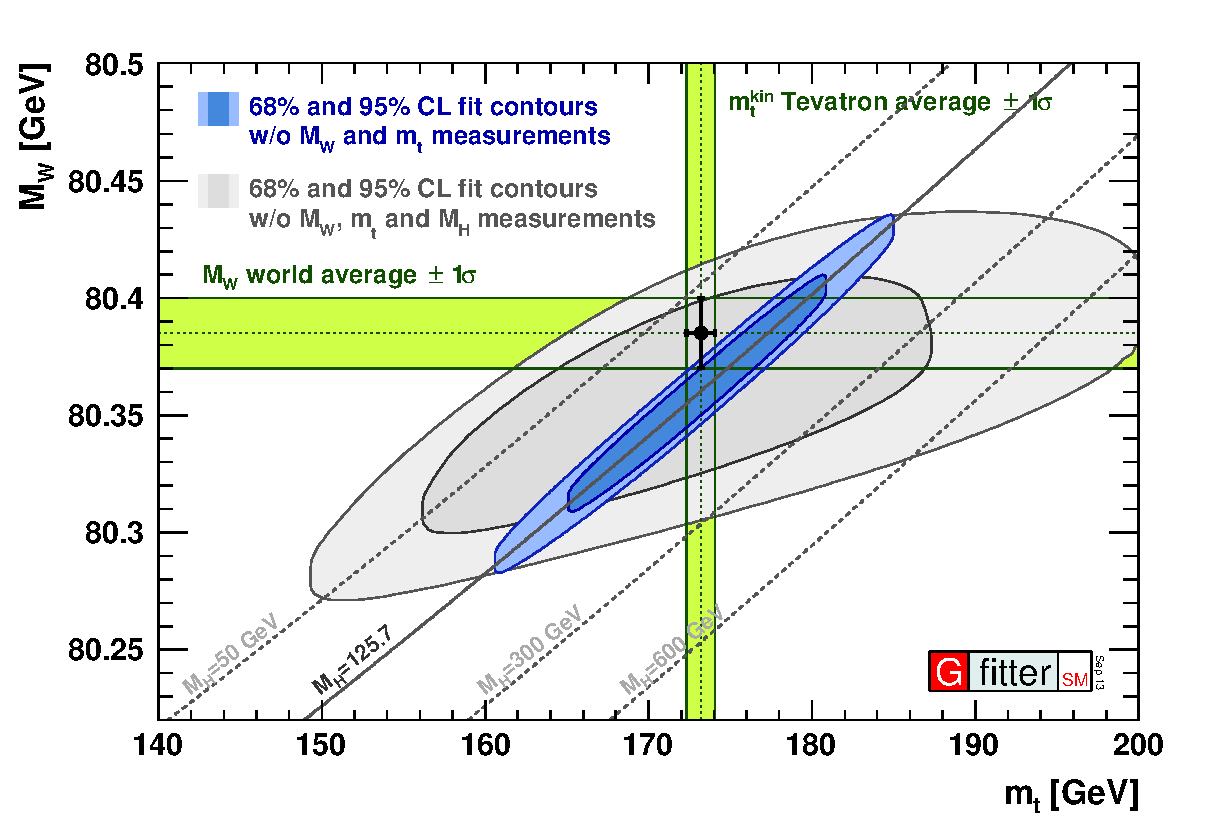
\includegraphics[width=0.6\textwidth]{theory/figures/W_vs_top.eps}}
        \caption[bla]{(a) Comparing fit results with direct measurements
of the free parameters of the SM, with the fit performed
with and without inclusion of the measured $M_H$. 
The pull values are defined as deviations between experimental 
measurements and theoretical calculations in units of the experimental uncertainty~\cite{Baak:2012kk}. 

        (b) Contours of 68\% and 95\% confidence level obtained 
from scans of fits with fixed variable pairs 
$M_W$ vs. $m_t$. The narrower blue and larger 
grey allowed regions are the results of the 
fit including and excluding the $M_H$ measurements, 
respectively. The horizontal bands indicate the 1$\sigma$
regions of the $M_W$ and $m_t$ measurements (world averages)~\cite{Baak:2012kk}. 
}
%Measured free parameters of the SM with the corresponding
%precision and the result of the consistency fit~\cite{Renton}.\label{fig:smparam}}
%\url{http://cerncourier.com/cws/article/cern/29076}}
\end{center}\end{figure}
 
In particular, the LEP experiments (ALEPH, DELPHI, L3 and OPAL) performed the measurements 
of the $Z$ boson mass with a precision of 0.0023\%, that made it one of the most 
precisely known quantities within the SM. %AAAAAAAAAAAAAAAAA \footnote{Note that the masses of the $W$ and $Z$ bosons are not predicted by the theory, but their ratio is (see Section~\ref{sec:ewlagr}).}. 
Furthermore, measurements of its total 
decay width and of its partial decay widths for all processes with a 
visible final state (i.e. different from $\nu\bar\nu$) allowed to set 
the number of light neutrino flavours to three, confirming the three-generation 
SM and excluding the possibility for a fourth family of leptons with masses
 lower than half of $m_Z$.

The penultimate discovery inside the SM has been the observation of the 
top quark in 1995 at the Fermilab's experiments CDF and 
D0~\cite{PhysRevLett.74.2626,PhysRevLett.74.2422}. 
The mass of the top quark resulted consistent with the predicted 
constraints (see Figure~\ref{fig:WtopMass}), 
thus confirming again the SM as an accurate framework. 
Figure~\ref{fig:history_mt} shows the evolution in
time of the top quark mass measurements and predictions,
while in Figure~\ref{fig:comb_mt} the best average
from measurements performed at the Tevatron experiments
CDF and D0 is given. All the properties that have been
observed (see for a review e.g.~\cite{Wicke:2010cg})
proved the top quark to be the SM up-type quark of the third generation.
At that point, and for almost 20 years, the last missing piece whose
absence could invalidate all the previous beautiful corroborations, was
the observation of a Higgs boson with a light mass for  self-consistency 
of the overall fit of data. When the LEP physics program was terminated,
direct searches gave, at 95\% CL, a lower limit of 114~\gev\ and an upper 
limit of 144~\gev\ on the mass of the Higgs boson~\cite{Barate:2003sz}. %,Renton}.

\begin{figure}[hbtp]
\begin{center}
	\subfigure[]{\label{fig:history_mt}
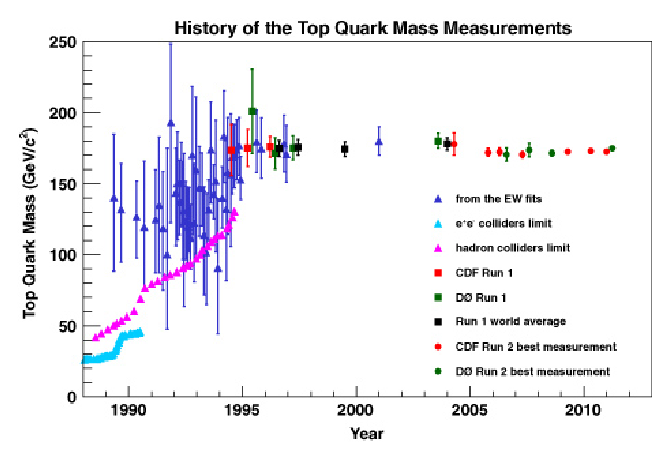
\includegraphics[width=0.6\textwidth]{theory/figures/rpp347183f01_online}}
%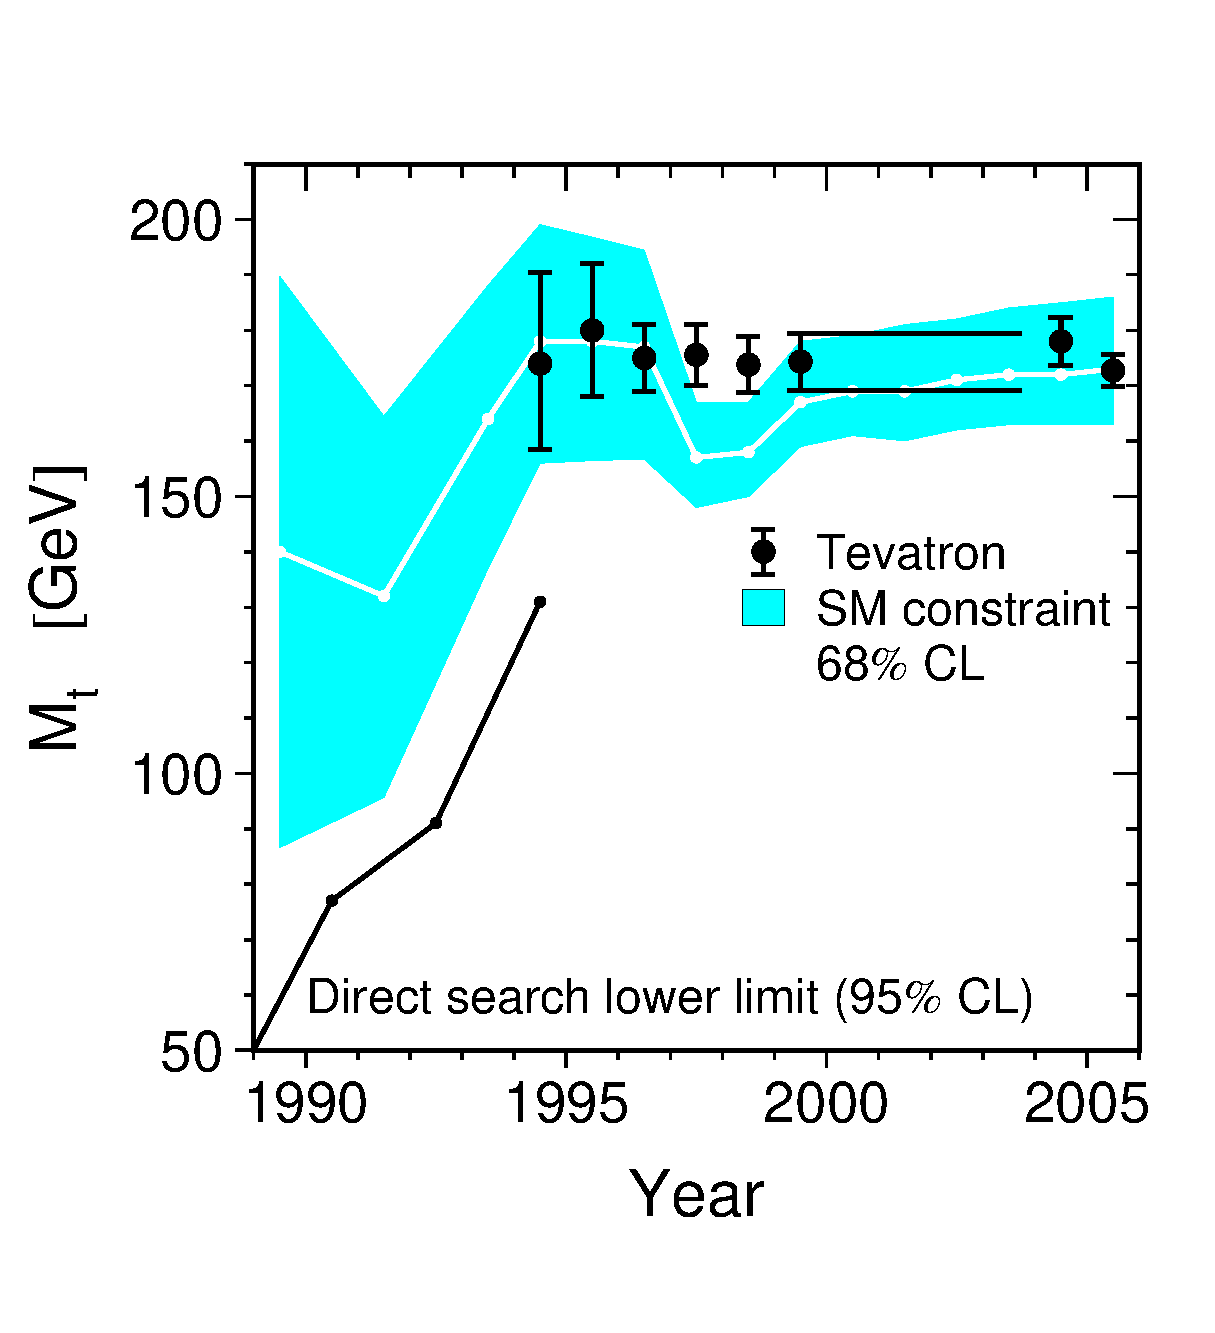
\includegraphics[width=0.5\textwidth]{theory/figures/history_mt}}
	\subfigure[]{\label{fig:comb_mt}
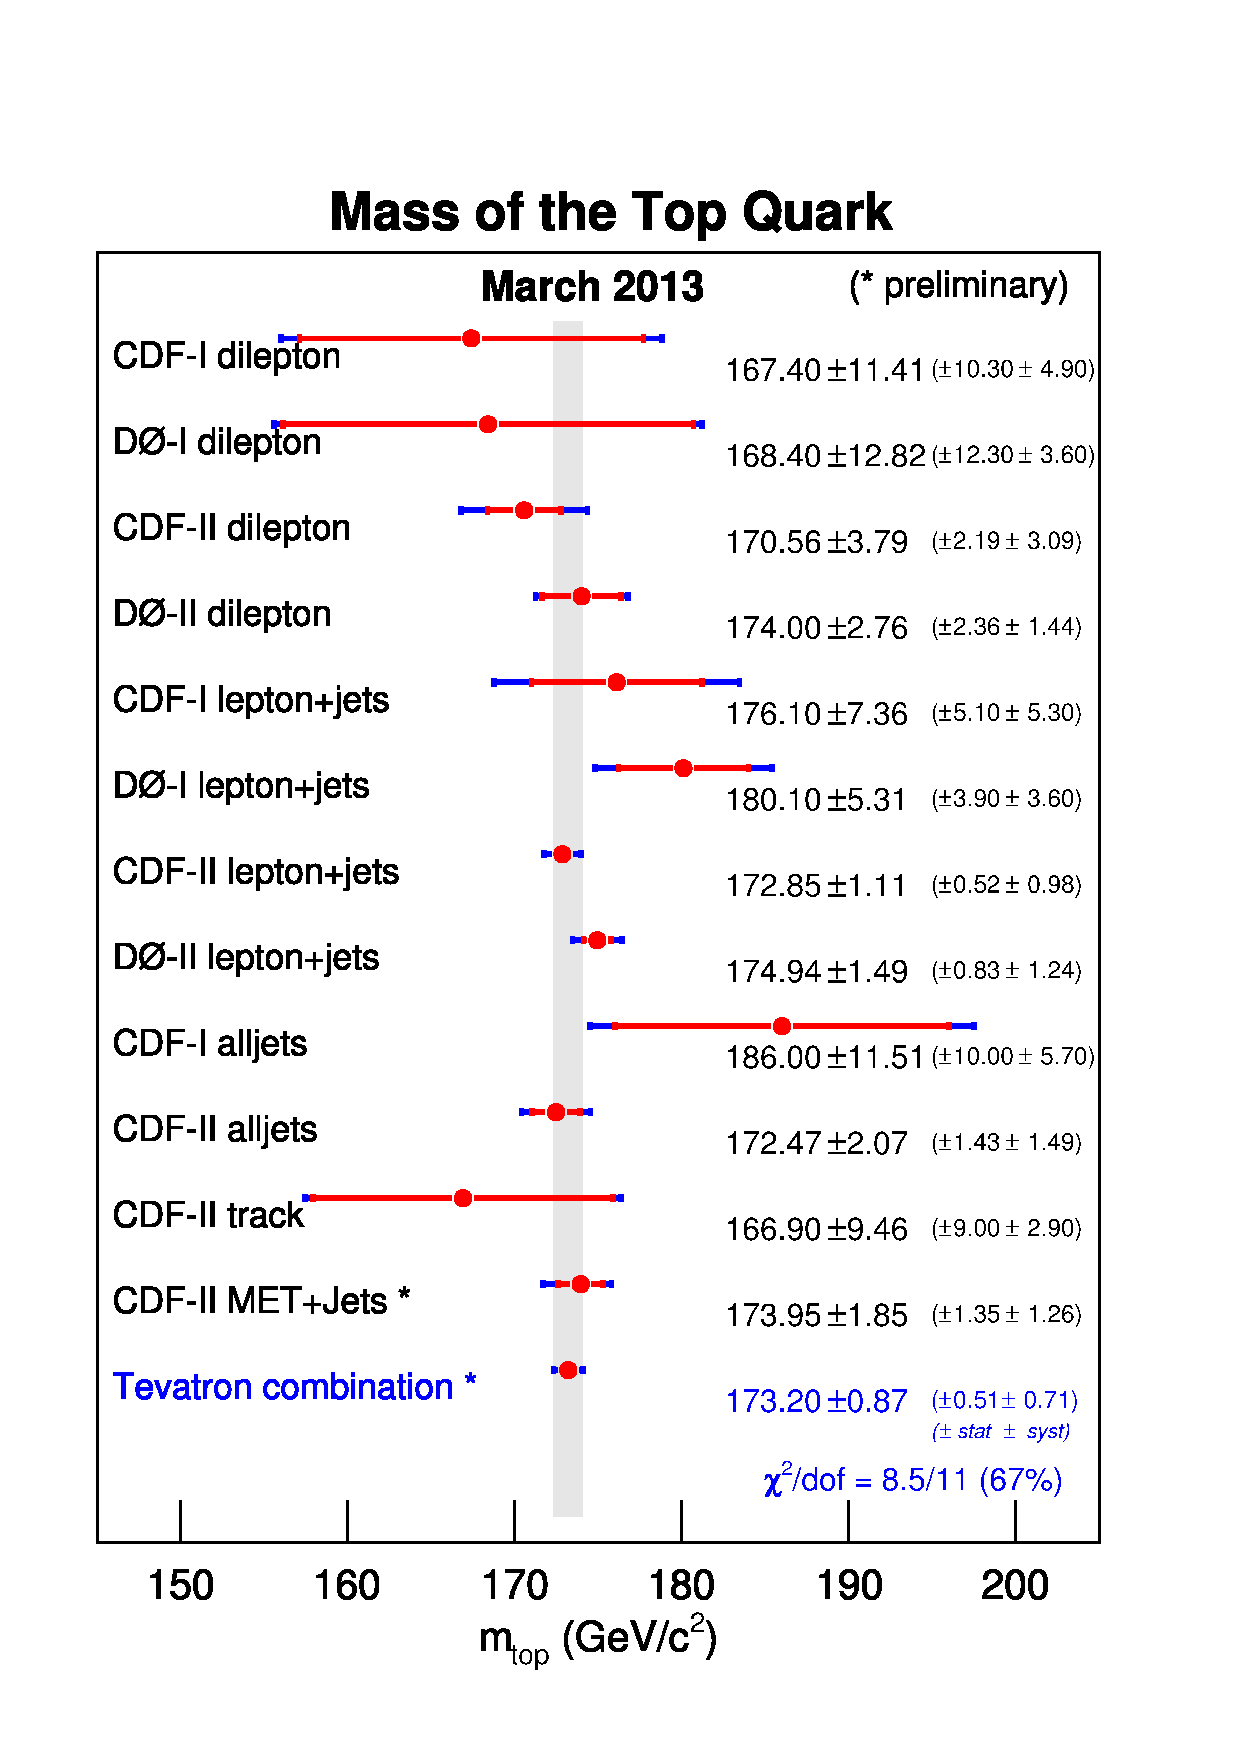
\includegraphics[width=0.35\textwidth]{theory/figures/TevMtWin13-2digit}}
\caption{(a) Evolution in time of the top mass prediction from
EW fits, of its exclusion limits at colliders and of its
experimental measurements at Tevatron~\cite{Galtieri:2011yd}.
(b) Summary of the top mass measurements at the CDF and D0 experiments
from Run-I (1992-1996) and Run-II (2001-present) 
in various channels and the resulting Tevatron average
 mass of the top quark~\cite{CDF:2013jga}.}
\end{center}
\end{figure}




Then LEP was dismantled, the LHC was built, and in 2012 
the ATLAS and CMS experiments
observed a new $\sim$125~\gev\ mass boson~\cite{2012gk,Chatrchyan201230}
with the same spin-parity as the one expected from a Standard Model
Higgs boson~\cite{Aad:2013xqa,CMShiggsspin}. 
A precise identification of this new particles, necessary
in order to say the final word about its nature (is it a Higgs boson?
Is it the Standard Model Higgs boson? Is it a ``new physics'' Higgs boson?),
is expected to come within the next decades of activity of the LHC and its
experiments. Up to the time of the writing of this dissertation, the most
recent results from the ATLAS and CMS experiments measuring the
properties of the new particle show consistency with a Standard
Model Higgs boson~\cite{Aad:2013wqa,CMS-PAS-HIG-13-005}.




\section{Unanswered questions and new physics quests}\label{sec:THquest}

In the case the new boson discovered in July 2012 
really is a Standard Model Higgs boson, there would
be no more arguments to contradict the Standard Model
as an {\it effective theory}. Indeed many facts, both 
in theory and experiments, hints that the Standard Model,
despite is great success in describing the interaction
of fundamental particles, might be just an approximation
at low energy regimes of a more complete theory.

One of the principal objections to the Standard Model as 
``the final theory'' is the high number of arbitrary parameters 
of the theory. In fact, 19 parameters are needed to fit 
data from experimental observations. 
Three of them  are the couplings of the gauge groups 
$g_3, g, g'$ for the strong, electromagnetica and weak 
interactions respectively, also written as: 
\begin{equation}\label{eq:couplings}
\alpha_{s}=\dfrac{g_{3}^{2}}{4\pi} ,\quad 
\alpha_{elm} = \dfrac{e^{2}}{4\pi} =  \dfrac{g^{2}\sin^{2}\theta_{W}}{4\pi}, 
\quad \sin^{2}\theta_{W} = \dfrac{(g')^{2}}{g^{2}+(g')^{2}}.
\end{equation}
Then, 13 parameters are associated with the nine charged 
fermion masses and the four parameters of the CKM matrix 
(three quark-mixing angles and one phase), 
two are needed to describe the Spontaneous Symmetry Breaking mechanism, 
i.e. the Higgs vacuum expectation value $v$ and 
the quartic coupling constant $\lambda$, and the last one is the 
QCD $\theta$ parameter. Additionally, if neutrinos are massive 
(as it is almost certain from neutrino oscillation observations, 
see e.g. \cite{Langacker:817840}) there will be even more arbitrary 
parameters describing their masses and their mixing. 
Furthermore, massive neutrinos cannot exist in the Standard
Model, where only left-handed neutrinos are predicted and thus
no Dirac mass term can appear\footnote{A way out of this
problem postulates a new type of neutrinos, namely 
{\it Majorana neutrinos}, in contrast to {\it Dirac neutrinos}.}.


%If, based on these considerations,  one assumes that 
The arbitrariety of parameters, and in particular of the
fermion masses, introduces what goes under the name of
{\it naturalness problem}. A ``natural'' theory is
characterized by free parameters with values at, more or
less, the same order of magnitude. This does not happen in
the Standard Model, where the top quark, as an example,
has a mass $\sim 10^5$ larger than the up quark.
This issue further develops as follows. If the 
Standard Model is valid only up to  an energy scale 
$\Lambda$ (which, if it's the Planck scale, differs
from the electroweak scale by $\sim 10^{17}$!), 
then the scalar Higgs boson mass 
should encounter radiative corrections from 
vacuum polarization diagrams (like the one in Figure~\ref{topLoop}) 
of the order of $\Lambda$ giving to the mass the 
value: %~\cite{dawson-1997}:
\begin{equation}\label{eq:higgsMass}
M_{H}^{2} \sim M_{H_{0}}^{2} 
+ \dfrac{\lambda}{4\pi^{2}} \Lambda^{2} 
+ \delta M_{H}^{2}. \end{equation}
If the mass counterterm $\delta M_{H}^{2}$ does not 
cancel the quadratically divergent contribution and 
if the cutoff scale is chosen as the Planck scale, then
\begin{equation}
M_{H}^{2} \sim 10^{32},\end{equation} 
i.e. many orders of magnitude bigger than the experimentally 
measured value coherent with the Standard Model 
and with the unitarity constraint. This  
is the \textit{hierarchy problem}, and 
could be fixed within the Standard Model by 
choosing a fine-tuned mass counterterm, a 
solution considered not really elegant also 
because fine tuning will be required for every 
order in the perturbative expansion\footnote{This 
problem does not arise with loop corrections to 
fermion masses, which are protected by chiral 
symmetry, nor with boson masses,
which are protected by gauge invariance. It
is, actually, an issue of scalar particles
like the Higgs boson.}. %and that's the reason why fermion masses are said to be ``natural''.} 


\begin{figure}[htb]\begin{center}
%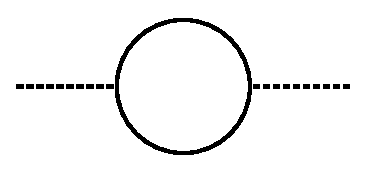
\includegraphics[width=.2\textwidth]{theory/figures/loop1}
\subfigure{ \def\svgwidth{0.25\textwidth}
\input{theory/figures/mod_loop1.eps_tex}}
\caption{The typical vacuum polarization diagram 
  for the Higgs is a top quark loop.}
\label{topLoop}\end{center}\end{figure}
%This argument looks the same of what made physicists pass from Fermi theory to Standard Model. In fact at that time the Fermi point like interactions were a good description of weak scattering processes of fermions $f+f\rightarrow f+f$, but the unitarity  predicted that at an energy $E_{crit} \sim 600$ GeV the theory would become inconsistent. Then it was found that new physics (the vector bosons of the Standard Model) was needed already from an energy scale about 100 GeV, maybe due to the small coupling constant of weak interaction. Now, the scattering process $W+W\rightarrow W+W$ has a scattering amplitude growing linearly to the self-coupling constant of the Higgs field $\lambda$. The formula for the critical energy is now related to the Higgs mass as \cite{Ho-Kim} $$\dfrac{E_{crit}}{v} = \exp\bigg(\dfrac{4\pi^{2}v^{2}}{3M_{H}^{2}}\bigg),$$ which for an higgs Higgs mass less than 150 GeV gives $E_{crit} \sim 10^{18}$, thus making the Higgs model valid up to that scale. However for an heavier Higgs with a mass about 700 GeV, such critical energy goes down to $10^{3}$ GeV.  It is to remark that in the electroweak interactions the Higgs contribution to radiative corrections is very low since is denoted by a logarithm function, thus giving low variations and not affecting the precision electroweak data. The meaning of this is, whatever the critical energy value will be, the Standard Model is an effective theory embedded in a more fundamental theory with $E_{crit}$ acting as a cutoff.

\begin{figure}[h!tb]\begin{center}
        \subfigure{ %\def\svgwidth{0.9\textwidth}
\input{theory/figures/mod_scales.eps_tex}}
	\caption{Typical length and energy scales
          of some of the fundamental parameters
          of the Universe.\label{fig:scales}}
\end{center}\end{figure}

Another disturbing feature of the Standard Model as it is 
is the lack of theoretical explanation for the generations 
of quarks and leptons to be exactly three, as suggested
(under certain assumptions) by precision measurements 
performed at LEP at the $Z$-pole ($\rts\sim 91$~\gev). 
From QCD comes the only constraint for quark generation
to be less that nine.

Cosmology and cosmological observations also challenge 
the Standard Model. The reason for baryon-antibaryon 
asymmetry is still not understood although we know 
that it is connected to  CP violation\footnote{The CP violating 
phase introduced in the CKM mechanism cannot, however, 
account for the total baryon-antibaryon asymmetry measured.}. 
Besides, astronomical observations~\cite{Ade:2013zuv} 
tell us that the energy density of the 
Universe is made only for a 4-5\% of ordinary baryonic 
matter, the other components being dark matter (20-25\%) 
and dark energy (70-76\%). Dark matter is non-baryonic 
matter that interacts only weakly and gravitationally and,
therefore, cannot be observed with telescopes but it
is revealed by its gravitational interaction with ordinary 
matter in space. 
It is now believed that Dark Matter is composed  of 
Weakly Interacting Massive Particles (WIMPs) whose 
masses range from a few GeV to a few TeV and  are 
not predicted within Standard Model. Dark energy instead is 
still more mysterious and maybe new physics will 
give some hints for its interpretation.

Another topic making the Standard Model likely to 
need improvements is the desire to go further in 
the unification of theories. Gravity is not 
implemented in the Standard Model, nor is available
a widely accepted quantum theory of gravity.
This is acceptable at the electroweak scale of 
few hundreds of GeV where the strength of gravity
is negligible, but its effect should become relevant 
going up to the Planck scale $\Lambda \sim 10^{19}$ GeV. 
Also, electroweak and strong forces forming the Standard 
Model gauge group $SU(2)_{L}\otimes U(1)_{Y}\otimes SU(3)_{C}$ 
are expected to unify at high energy since their coupling 
constants are running constants dependent on the energy 
scale (Figure~\ref{running}, $\alpha^{-1}_{i} = g^{2}_{i}/(4\pi)$). 
\begin{figure}[htb]\begin{center}
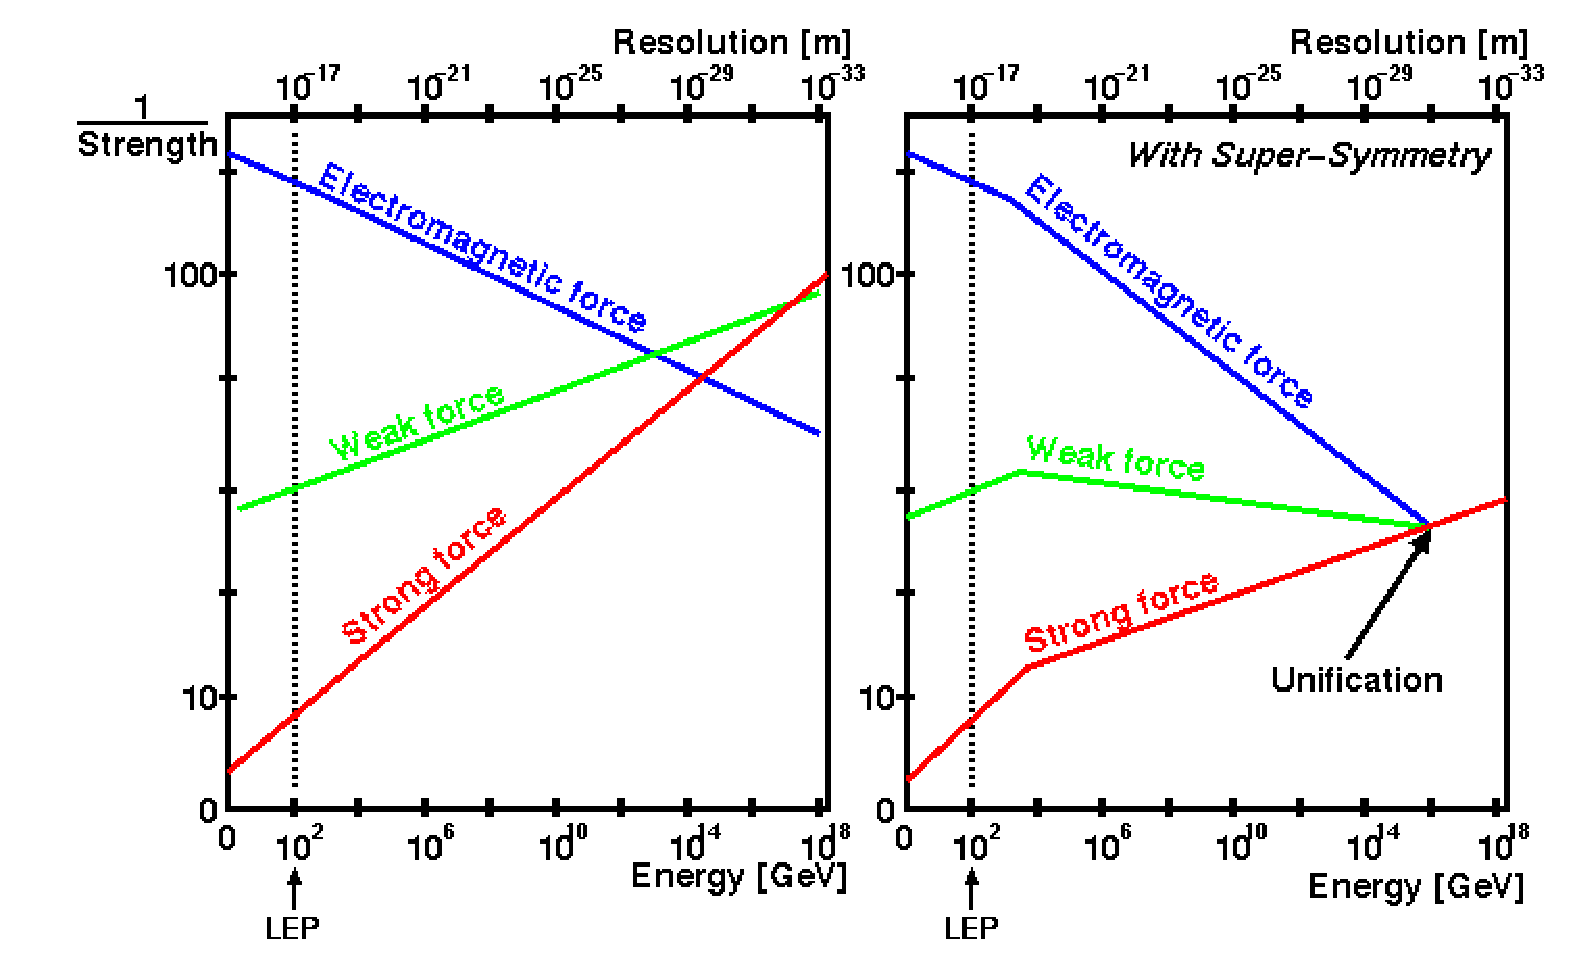
\includegraphics[width=.8\textwidth]{theory/figures/running_coupling}
\caption{Running coupling constants in the Standard Model (left) and 
in a hypothetical Supersymmetric Model (right, see Section~\ref{sec:susy}) 
as functions of the renormalization scale (picture from \url{http://scienceblogs.com},
original credits unknown). The energy scale explored at LEP is marked
on the two figures and corresponds to $10^2$~\gev. The LHC is able to
go just one order of magnitude further.}
\label{running}\end{center}\end{figure}

In the following some ``beyond-Standard Model'' (BSM) theories
proposed to solve most of the issues illustrated
before are briefly illustrated.

\subsection{Supersymmetry}\label{sec:susy}

Since Supersymmetry~\cite{Dawson:1996cq} is one of the most popular
BSM scenarios, having many trustful supporters even
now that after the first LHC run no trace of it
has been found, a brief explanation of its concepts
is included in this dissertation.

The basic idea is to postulate the invariance 
of the theory under a symmetry operation which 
trasforms fermionic fields into bosonic fields 
(and viceversa), called \textit{supersymmetry}. 
In this theory to each fermionic or bosonic 
degree of freedom of the Standard Model is associated a 
``superpartner''. These superpartners have all 
of the quantum numbers identical to the corresponding 
Standard Model particles, except for the spin quantum number 
transformed as $s' = |s - 1/2|$. Thanks to the 
presence of superpartners, the Fermi statistics 
allows to write the new version of Equation~\ref{eq:higgsMass} as:
\begin{equation}
\label{eq:higgsMassSUSY}
M_{H}^{2} \sim M_{H_{0}}^{2} + \dfrac{g_{F}^{2}}{4\pi^{2}} (\Lambda^{2} + m_{F}^{2} ) - \dfrac{g_{S}^{2}}{4\pi^{2}} (\Lambda^{2} + m_{S}^{2} ),
\end{equation} 
where the subscripts $F$ and $S$ indicate respectively 
fermionic and scalar degrees of freedom. If $g_{F} = g_{S}$ 
and masses are equal as in an unbroken supersymmetry scenario, 
the $\Lambda^2$ terms cancel and the hierarchy problem is solved. 
However, since no superpartners of known particles 
have been observed,  supersymmetry must be a broken 
symmetry and sparticles masses have to lie in an 
energy range not yet accessed by experiments.

%The simplest and most popular supersymmetric model is called the Minimal Supersymmetric extention of the Standard Model (MSSM). In the MSSM, $SU(2)_{L}\otimes U(1)_{Y}\otimes SU(3)_{C}$ gauge symmetries are still valid, but particles are now organized in \textit{Chiral Superfields} (formed by a complex scalar field and a fermion field with two components) and \textit{Vector Superfields} (made of a massless gauge field and two-component fermion field named \textit{gaugino}). Even if the scalar superpartners of fermions do not feature handedness, the chirality is formally assigned as the one of the standard particles in the supermultiplet. Then, for every family of quarks and leptons of the SM, a superfield made of an $SU(2)_{L}$ doublet of fermions and an $SU(2)_{L}$ doublet of scalars is defined ($\hat Q_{1,2,3}$ for quarks, $\hat L_{1,2,3}$ for leptons), as well as one superfield of right-handed anti-leptons and anti-sleptons ($\hat E_{1,2,3}$) and two superfields of right-handed anti-quarks and anti-squarks ($\hat U_{1,2,3}$ and $\hat D_{1,2,3}$). There are then two other Chiral Superfields in the Higgs sector ($\hat H_{u,d}$) and three Vector Superfields made of the gauge bosons and their relative superpartners ($\hat{G}^{a},\ \hat{W}^{i},\ \hat{B}$). 
%As can be seen in the summary of the MSSM supermultiplets in Table \ref{tab:supermultiplet}, an additional Higgs doublet needs to be postulated. The reason is that while in Equation \ref{eq:higgsMassSUSY} the term from scalar squarks cancels, in the similar equations for the fermions masses, where anomalies are automatically  cancelled within the SM, the newly introduced term from the Higgsino fermionic field remains. Thus another Higgs doublet with opposite $U(1)$ quantum number is defined. Furthermore, having two Higgs doublets is in general also required in order to give masses to both up and down type quarks in Supersymmetric theories. The two Higgs doublets with their eight components yield four extra bosons with respect to the SM, i.e. we get five physical Higgs bosons ($h^{0}, H^{0}, A^{0}, H^{\pm}$) and the relative superpartners, the fermionic Higgsinos. Gauginos mix  with Higgsinos resulting in the eight mass eigenstates: $\tilde{\chi}^{\pm}_{1,2}$ (the \textit{Charginos}) and $\tilde{\chi}^{0}_{1,2,3,4}$ (the \textit{Neutralinos}). After defining the superfields it is possible to construct the Lagrangian of the MSSM; a very clear step-by-step  pedagogical description for this task is given in Ref.~\cite{Martin}.

Supersymmetry also provides a natural candidate
for Dark Matter, the Lightest SUSY Particle (LSP), 
which, in a {\it R-parity}\footnote{The quantum number 
\textit{R-Parity} is defined as $R \equiv (-1)^{3(B-L) + 2s}$
to prevent lepton and baryon numbers from being violated.
It has value $+1$ for all Standard Model particles 
and $-1$ for their superpartners.} 
conserving scenario~\cite{Martin:1997ns},
would be stable, weakly interacting and neutral.



\subsection{Fourth generation SM4}\label{sec:sm4}

One of the simplest 


\subsection{Little Higgs}\label{sec:littlehiggs}

\begin{figure}[htb]\begin{center}
\subfigure{ \def\svgwidth{0.25\textwidth}
\input{theory/figures/mod_loop1.eps_tex}}
\subfigure{ \def\svgwidth{0.18\textwidth}
\input{theory/figures/mod_loop2.eps_tex}}
\label{fig:susyloops}\end{center}\end{figure}

\subsection{Extra-dimensions}\label{sec:extradimensions}





\section{Going beyond the SM with vector-like quarks}\label{sec:THvlq}

\cite{AguilarSaavedra:2009es,Martin:2009bg}



\clearpage{\pagestyle{empty}\cleardoublepage}
\clearpage{\pagestyle{empty}\cleardoublepage}

\chapter{The ATLAS experiment at the Large Hadron Collider}\label{chap:atlas}

The time when particle physics experiments could fit in one's
loft is well passed, if it ever existed. The reason is simple,
as the deeper we want to investigate matter, the highest the energy
we need. According to the Standard Model, we now know all the
particles composing ordinary matter present in nature, so if we
want to see something new, we need to produce it. The way to
do it is suggested by one of the fundamental principles of relativity,
$E=mc^2$, according to which we can smash massive particles
and observe what other kind of matter comes out of the
available energy.
Soon enough after the discovery of the muon, after observing all
the observable from cosmic rays, physicists
started to do that using particle accelerators, the last of
them in history being the Large Hadron Collider.

The Large Hadron Collider, built to collide protons at a \cme\ of 14~\tev, 
is the world's highest energy particle accelerator, overcoming the Tevatron
proton-antiproton collider where the top quark was discovered
in 1995~\cite{PhysRevLett.74.2422,PhysRevLett.74.2626}.
The ATLAS experiment is one of the collaborations that take advantage
of the collisions provided by the Large Hadron Collider,
and has been conceived to pursuit a challenging physics program with,
at the head of the list, the discovery of the Higgs boson, achieved
in 2012~\cite{2012gk}.

In the following Chapter we will briefly describe the main features of 
the accelerator and with some more details the ATLAS detector, 
both located at the CERN laboratories in Geneva,
Switzerland.


\section{The Large Hadron Collider at CERN}\label{sec:lhc}

The LHC program was approved by CERN Council in 1994, followed by the approval of
the four main experiments: ATLAS~\cite{Aad:2008zzm} and CMS~\cite{cms}
in 1996; ALICE~\cite{alice} in 1997; LHCb~\cite{lhcb} in 1998.
Works towards the installation of the most powerful particle accelerator of the world
started when the Large Electron Positron Collider (LEP) was dismantled in 2000 to 
give up its place in the tunnel to the LHC, which was then fully operational by 2008.

The ATLAS experiment~\cite{Aad:2008zzm} is situated at Point~1 along the Large Hadron Collider 
(LHC)~\cite{lhc} 27~km long ring (Figure~\ref{fig:nicepics}).
The accelerator
tunnel can reach an underground depth of 175~meters and is spread between Swiss
and French territory, while the cave where ATLAS is allocated is about 100~meters 
underground in the CERN Swiss site of Meyrin.

\begin{figure}[tb]\begin{center}
	\subfigure[]{\label{fig:atlasmural}
  	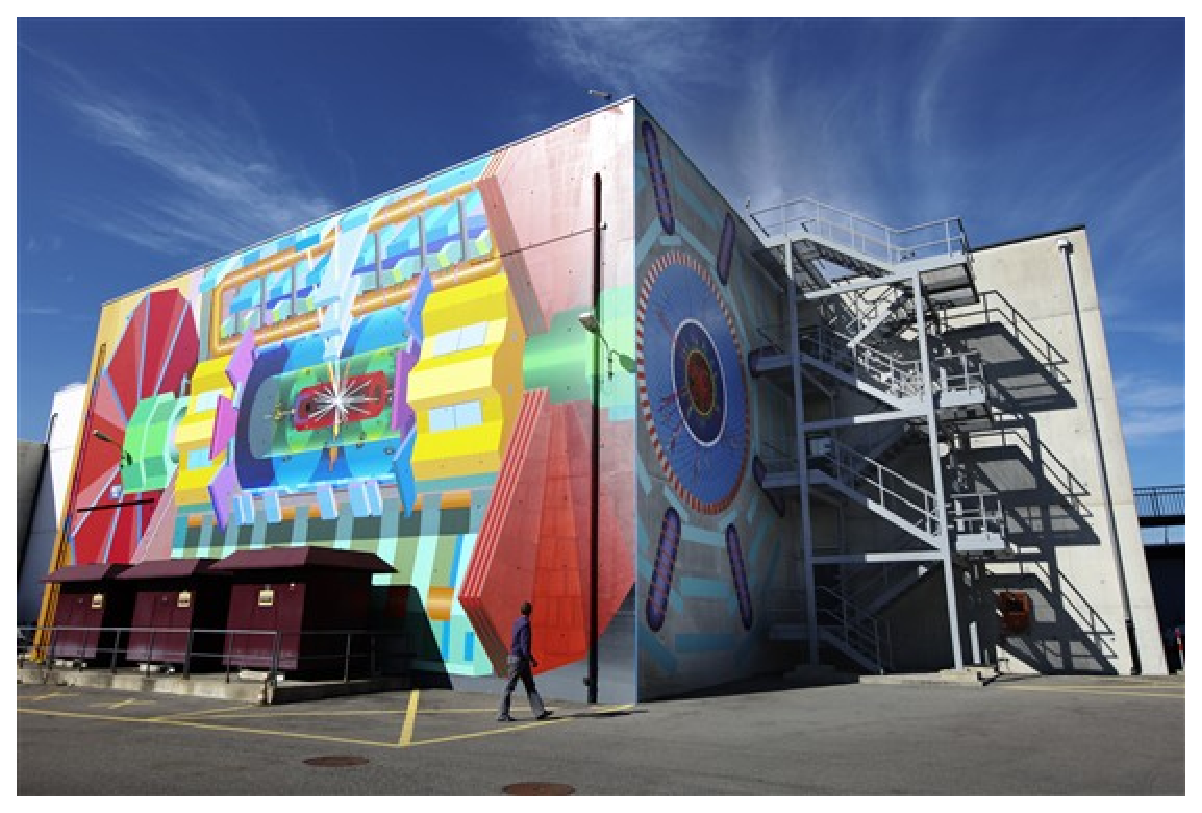
\includegraphics[width=0.47\textwidth]{detector/figures/mural}}
	\subfigure[]{\label{fig:lhcdraw}
  	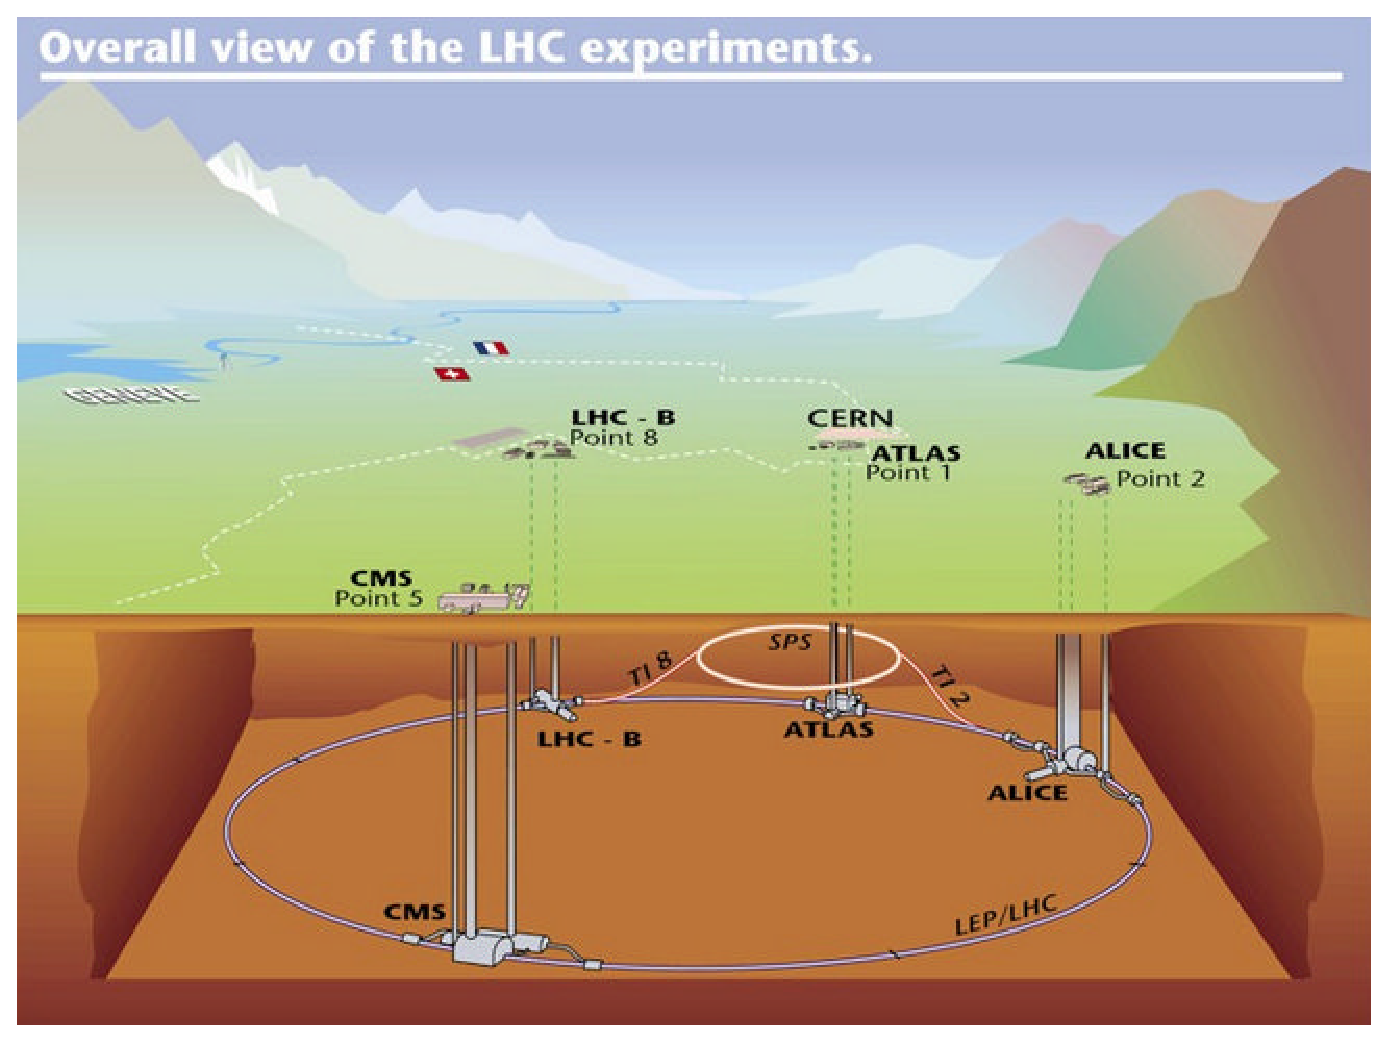
\includegraphics[width=0.42\textwidth]{detector/figures/lhc_diagram}}
	\caption[bla]{Left: View of Point 1, just above the ATLAS cavern, with a mural painting 
        of the detector, reproduced at a scale of about 1:3
        by artist Josef Kristofoletti\footnotemark.
        Right: A drawing of the LHC complex.\label{fig:nicepics}}
\end{center}\end{figure}

The collider accelerates protons up to 4~\tev, but is designed to reach 7~\tev\ per beam
when it will be operated at his full potential. This energy is achieved
through various steps, shown in Figure~\ref{fig:lhcring}.
To start with, protons are extracted from Hydrogen gas and injected in the first machine, the linear 
accelerator LINAC2 that starts the acceleration chain. When protons reach
an energy of 50~\mev\ they are injected into the Proton Synchrotron Booster
(PSB) and accelerated up to the energy of 1.4~\gev. The second circular
accelerator, the Proton Synchrotron (PS) brings the energy of the protons
to 25~\gev\ previous to injecting them into the last machine before the LHC,
the Super Proton Synchrotron (SPS). Protons of 450~\gev\ finally enter the
LHC where they are boosted to energies of up to 4~\tev.
The four main LHC experiments are shown on the collider ring.

\begin{figure}[tb]\begin{center}
	\subfigure{
  	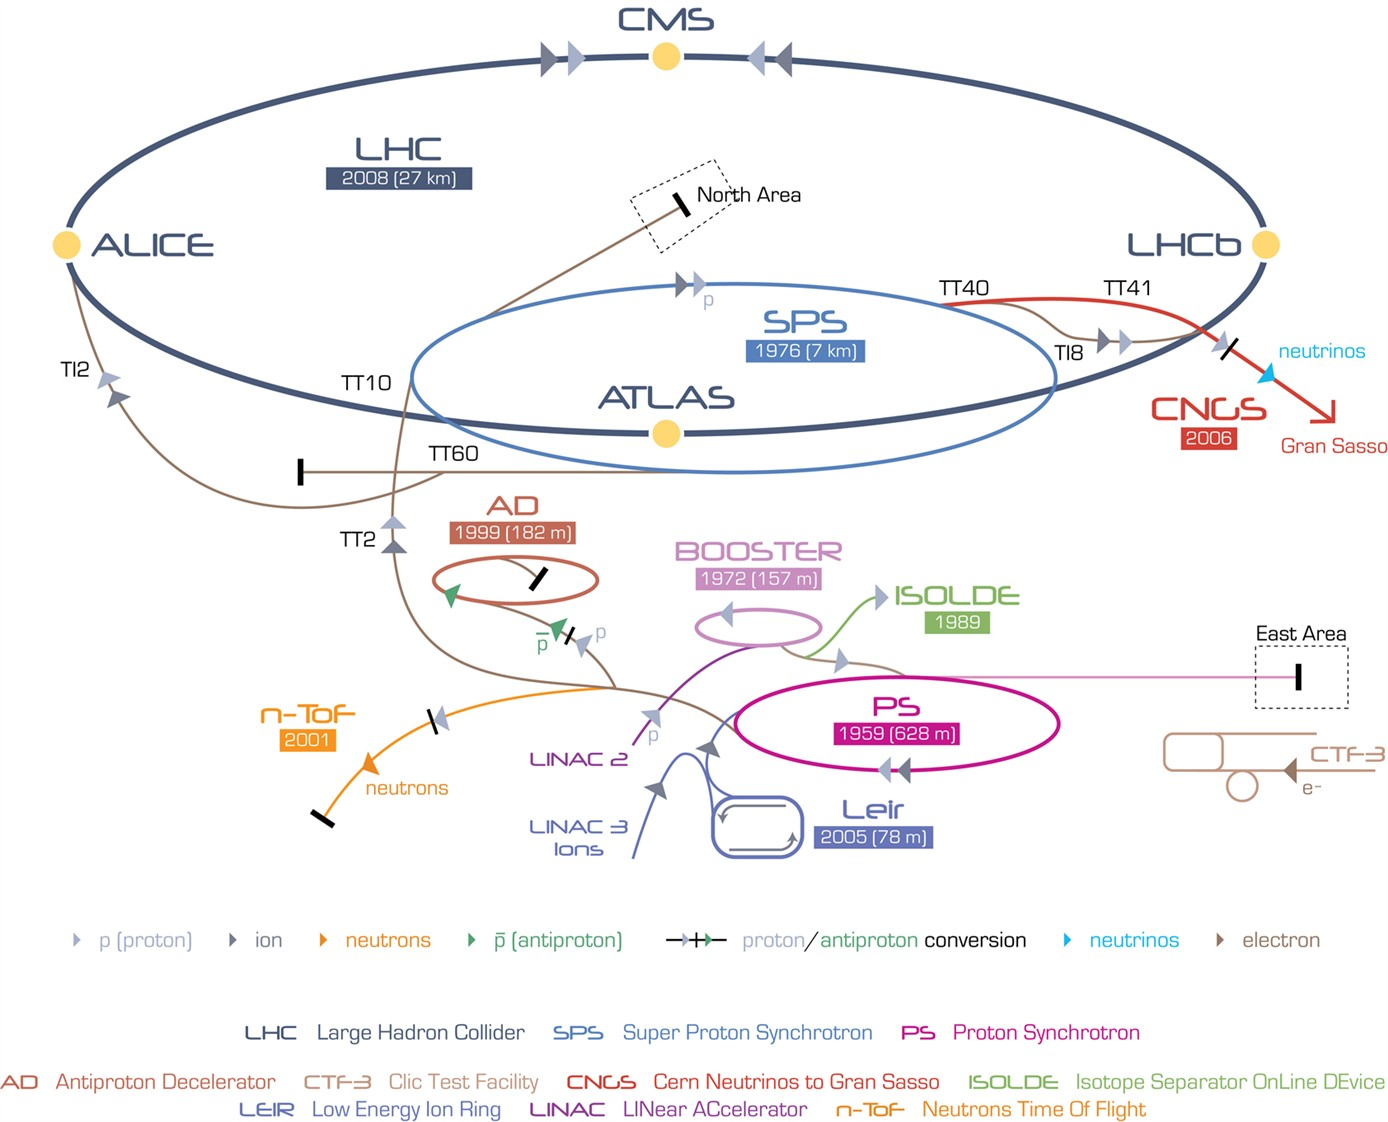
\includegraphics[width=0.8\textwidth]{detector/figures/ring.eps}}
	\caption{A schematic showing the accelerator complex at CERN.\label{fig:lhcring}}
\end{center}\end{figure}


\footnotetext{More info at: \url{http://www.atlas.ch/mural/}.}

The LHC is composed of eight arcs 2.7~km long, each of which contains 154 dipole 
magnets, whose function is to  bend the beams along the circular trajectory, and
49 quadrupole magnets, that focus the beam. These superconducting magnets operate
at a temperature of 1.9~K, maintained by means of liquid Helium vessels.
Eight insertions are placed inbetween the arches. Each insertion has a specific
role that characterizes its design and can be injection, beam dumping, beam cleaning,
or ``physics'', i.e. make the beams collide within an experiment.

First proton beams were circulated on 10th September 2008 and right on the verge of
getting the first collisions at a \cme $\rts=900\gev$ nine days later, an electrical
connection joining superconducting wires of a dipole and a quadrupole
failed. This caused the release of liquid Helium in the insulating vacuum,
resulting in an explosion that severely damaged the machine.
After more than one year devoted to repair the damage and consolidate the security,
on 30th November 2009 the LHC became the world's highest energy particle 
accelerator\footnote{\url{http://press.web.cern.ch/press/PressReleases/Releases2009/PR18.09E.html}}:
\begin{quotation}\small
Geneva, 30 November 2009. CERN's Large Hadron Collider has today become the world’s highest energy particle accelerator, having accelerated its twin beams of protons to an energy of 1.18 TeV in the early hours of the morning. This exceeds the previous world record of 0.98 TeV, which had been held by the US Fermi National Accelerator Laboratory’s Tevatron collider since 2001. It marks another important milestone on the road to first physics at the LHC in 2010.
\end{quotation}


One of the main characteristics for an accelerator is the luminosity, the 
instantaneous luminosity $\mathcal L$ being defined as 
\begin{equation}\label{eq:lumiN}
\mathcal{L}\times\sigma=\dfrac{dN}{dt}=f\times n\dfrac{N_1\times N_2}{A}\times\sigma.
\end{equation} 
Here $dN/dt $ is the event rate of a certain process and $\sigma$ is its cross 
section. This rate is directly proportional to the the frequency $f$, the number 
of bunches $n$ and the number of particles in the two bunches $N_1, N_2$, and
inversely proportional to the beam cross-section $A$.
The instantaneous luminosity is measured by dedicated subdetectors that are
described in Section~\ref{sec:forward}.

Integrating over the accelerator active time (a ``fill'', when stable beams are kept
colliding) gives the \textit{integrated luminosity}, relating the total number 
of produced events $N_{tot}$ to the cross-section:
\begin{equation}\label{eq:intLumi}
\int \mathcal L dt  = \dfrac{N_{tot}}{\sigma}.
\end{equation}




%http://accelconf.web.cern.ch/accelconf/IPAC2013/papers/moyab101.pdf
%http://cerncourier.com/cws/article/cern/54381

\begin{table}\centering
	\begin{tabular}{lllll}\toprule
        Parameter                       & designed      &       2010 &  2011     &   2012\\ \midrule
        Beam energy (\tev/c)            & 7             & 3.5        & 3.5       & 4    \\
        Beta function $\beta*$ (m)      & 0.55          & 2.0/3.5    & 1.5/1.0   & 0.6  \\
        Max. No. bunches/beam           & 2808          & 368        & 1380      &1380  \\
        Max. No. protons/bunch          & 1.15$\times10^{11}$ & 1.2$\times10^{11}$ & 1.45$\times10^{11}$ & 1.7$\times10^{11}$ \\
        Bunch spacing (ns)              & 25            & 150       & 75/50        & 50 \\
        Peak luminosity (\cmm2\sm1)     & 1$\times10^{34}$& 2.1$\times10^{32}$& 3.7$\times10^{33}$& 7.7$\times10^{33}$\\
        Emittance $\varepsilon_{n}$ ($\mu$rad)&3.75     &   2.0      & 2.4      & 2.5   \\
        Max. $<\mu>$                    & 19            & 4             & 17         & 37       \\
	\bottomrule\end{tabular}\caption{Overview of some parameters for the LHC performance comparing the design values with their time
        evolution during the first long run operation in 2010-2013~\cite{Lamont}.}\label{tab:lhcpar}
\end{table}

\begin{figure}[tb]\begin{center}
	\subfigure[]{\label{fig:intlumi}
  	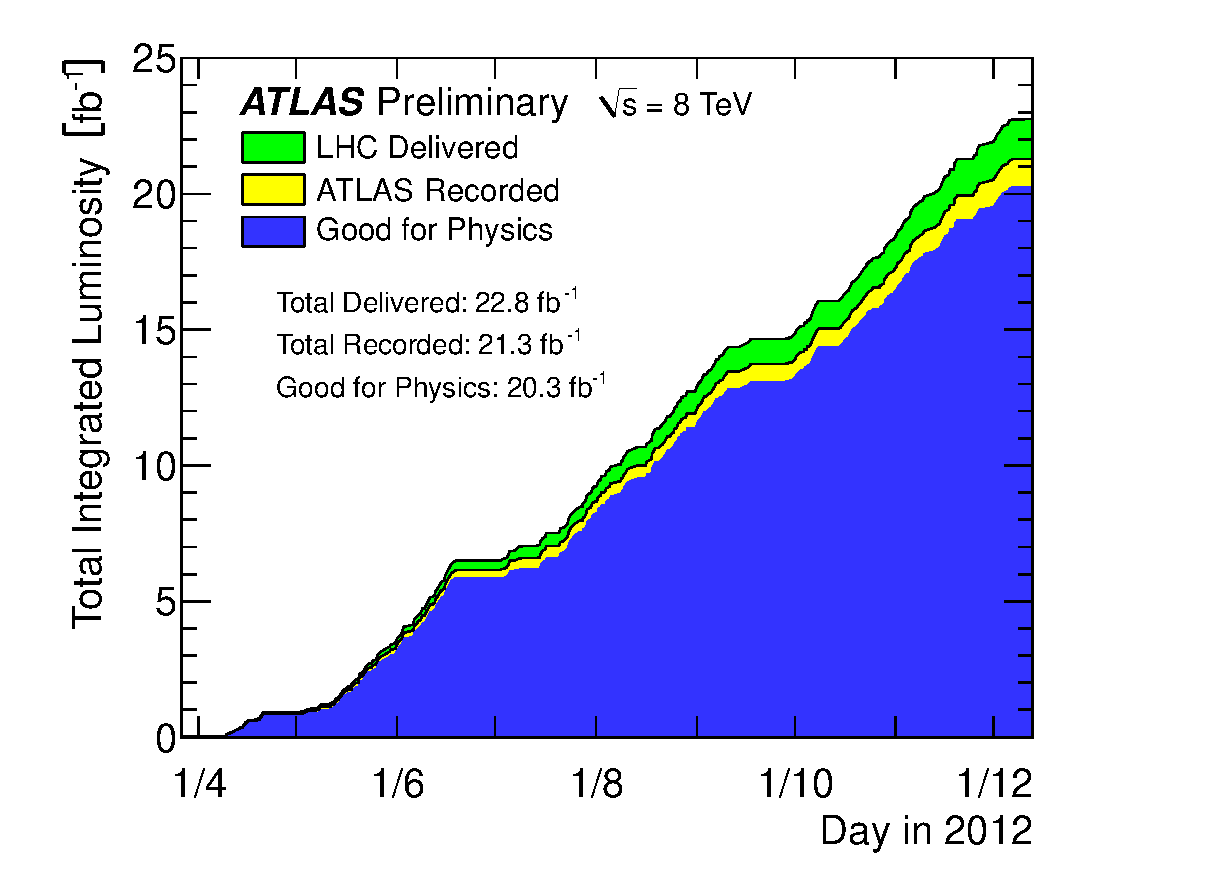
\includegraphics[width=0.48\textwidth]{detector/figures/intlumivstime2012DQ}}
	\subfigure[]{\label{fig:mu}
  	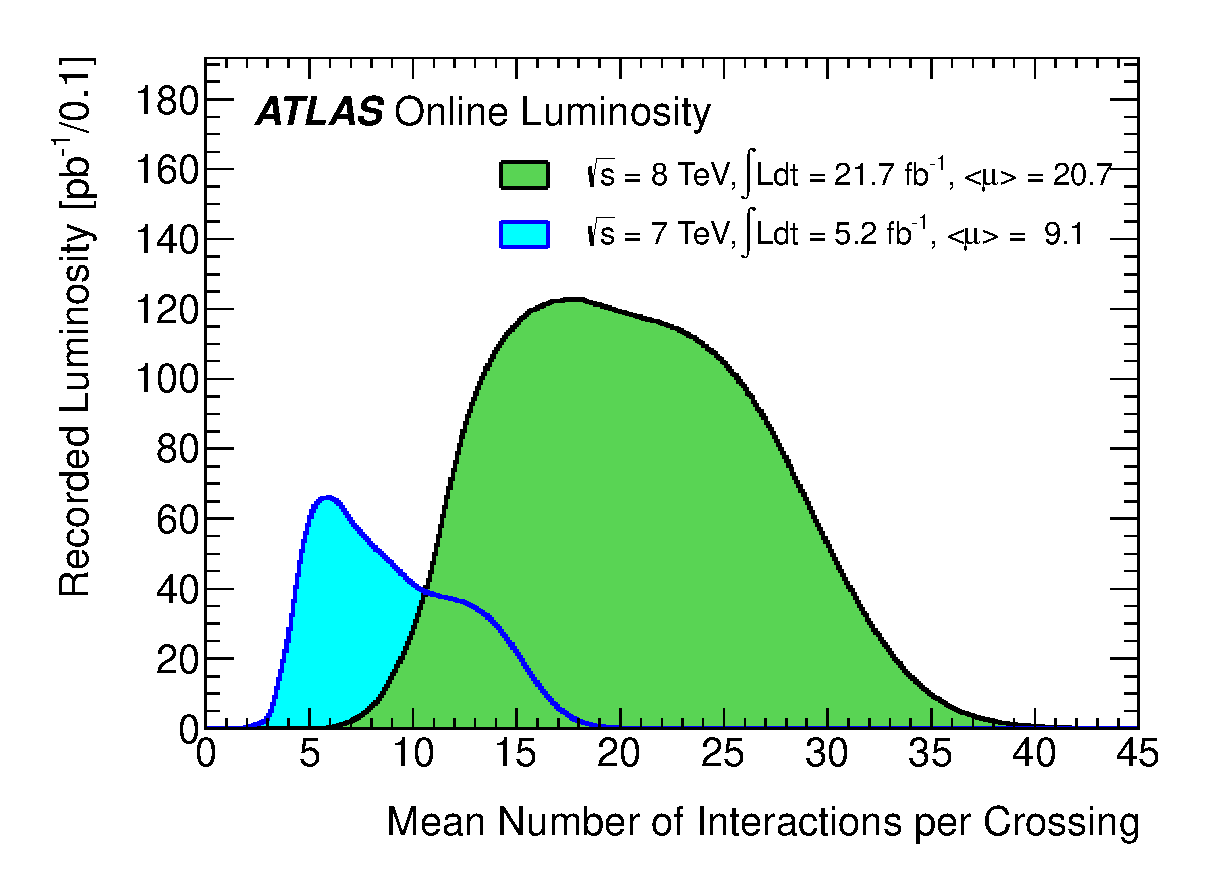
\includegraphics[width=0.48\textwidth]{detector/figures/mu_2011_2012-dec}}
	\caption{(a) Total integrated luminosity versus time delivered by the LHC to ATLAS (in green), recorded by the experiment 
        (in yellow) and selected as ``good data'' for analysis (in blue) for p-p collisions at \rts=8~\tev.
        (b) Mean number of interactions per beam crossing during 2011 and 2012 LHC runs, where 
        $\mu = \mathcal L\times \sigma_{\rm inelastic}/f$ depends on the instantaneous luminosity $\mathcal L$, the p-p inelastic
        cross section $\sigma_{\rm inelastic}$ and the revolution frequency $f$.~\cite{lumi}}
%Number of Interactions per CrossingMore details on this can be found in arXiv:1101.2185. 
\end{center}\end{figure}

In 2010 ATLAS collected about 45~\ipb of p-p collision data at \rts=7~\tev, and in
2011 reached about 5~\ifb of the same data.
In 2012, with  \rts=8~\tev\ collisions, LHC reached a peak luminosity of 7.7$\times10^{33}$~\cmm2\sm1\ which is
more than half the design luminosity, as shown in Table~\ref{tab:lhcpar} together
with other parameters relevant for the accelerator performance. 
Over 2012, the last
year of data taking before the long shutdown\footnote{LHC terminated the p-p program
at the end of 2012, operated proton-heavy ion collisions for two months at the beginning
of 2013 and then stopped for what is called the first long shutdown. During this two-years
time the accelerator and the experiments as well will undergo substantial maintenance and 
upgrade works, in order to be re-operated in 2015 with higher performance at a higher
\cme for particle collisions.},
ATLAS collected about 20~\ifb\ of p-p collision data at \rts=8~\tev.
Figure~\ref{fig:intlumi} shows the delivered luminosity from the start of stable beams until beam dump and the luminosity recorded by
ATLAS during stable beam conditions, the difference with respect to the delivered luminosity being due to Data AQuisition (DAQ)
inefficiencies. Of the recorded luminosity, only a part is usable for analysis, and is what is called ``good data'', i.e. 
the data that satisfy Data Quality (DQ) requirements assessed after reprocessing (see Section~\ref{sec:daq}).

In order to increase the luminosity LHC operates with a high number of protons per bunch as well as a high
 number of bunches per beam and reduces the inter-bunch latency time.
This overall defines a set of challenges that physics analysis will face associated to the high luminosity.
Even at the detector design stage, the high frequency of collision environment foreseen influenced
the choice of radiation resistance material for the experiment sub-systems. Concerning directly the physics
%instead we can list the main problematics as being \textit{underlying events} and \textit{pile-up}
instead, the main problematic is \textit{pile-up}.

Pile-up events are distinguished between \textit{in-time} and \textit{out-of-time} pile-up. The first ones come 
from the multiple inelastic scatterings of protons in the same bunch, as if we consider a cross-section of 80~mb
at the nominal luminosity of $10^{34}$~\cmm2\sm1 the number of events per second will be something like
a billion. This translate, at a collision frequency of one crossing every 25~ns, to about 20 interactions per
crossing that will be detected simultaneously. A useful observable to estimate in-time pile-up is
the number of reconstructed primary vertices (see Section~\ref{sec:primaryvertex}) $N_{\rm PV}$.
In addition, on the other hand, the inter-bunch time interval is so short
that the electronics reading the detector might not keep up with the frequency of collisions, leading to the
cumulation of events that happened in different beam crossings. This is the effect we refer to as 
out-of-time pile-up, and a good estimator for it is the average number of p-p interactions
per bunch crossing at the time of the event, $<\mu>$, which recalling Equation~\ref{eq:lumiN} is defined as:
\begin{equation}\label{eq:mu}
<\mu> = \dfrac{LA}{nf},
\end{equation}
with $L$ being the average instantaneous luminosity over a time period $\Delta t\gg 600$~ns.
The maximum values reached by the variable $<\mu>$ during the three years of data taking
are reported in Table~\ref{tab:lhcpar}.

Finally, ATLAS makes use of a three-level trigger system (described in Section~\ref{sec:trigger}) to identify
and record only the events of interest, while the pile-up issues are dealt with at the analysis 
reconstruction level.



\section{The ATLAS detector}\label{sec:atlas}

ATLAS (A Toroidal LHC ApparatuS)~\cite{Aad:2008zzm} is a general purpose experiment
aimed at exploring a vast range of physics scenarios and designed to measure the particles
produced in p-p collisions at the LHC at unprecedented energies and instantaneous luminosities. 
It is the biggest detector of its kind ever built (it's 46~m long and 25~m high) is characterized by
a full coverage of the space around the p-p interaction point and complete
containment of the particles produced in the collision. Different subsystems are
layered concentrically one after the other, each of them pursuing a specific task. 
Right around the interaction point
(IP) where the LHC makes protons collide there is the Vertex Detector, reconstructing
charged particles trajectories that are bent by the first solenoid magnet surrounding
the Vertex Detector. Particles going through it then encounter the two calorimeter systems,
the Electromagnetic and the Hadronic one. Muons are the only particles that will pass
the calorimeters material (beyond neutrinos) and a dedicated Muon Spectrometer is the last
piece of detector, embedded in a huge toroidal magnet. The detector complex is presented
as a schematic in Figure~\ref{fig:atlas}, and a drawing of particle detection in the various
subdetector systems is shown in Figure~\ref{fig:detection}. 

\begin{figure}[htb]\begin{center}
	\subfigure{
  	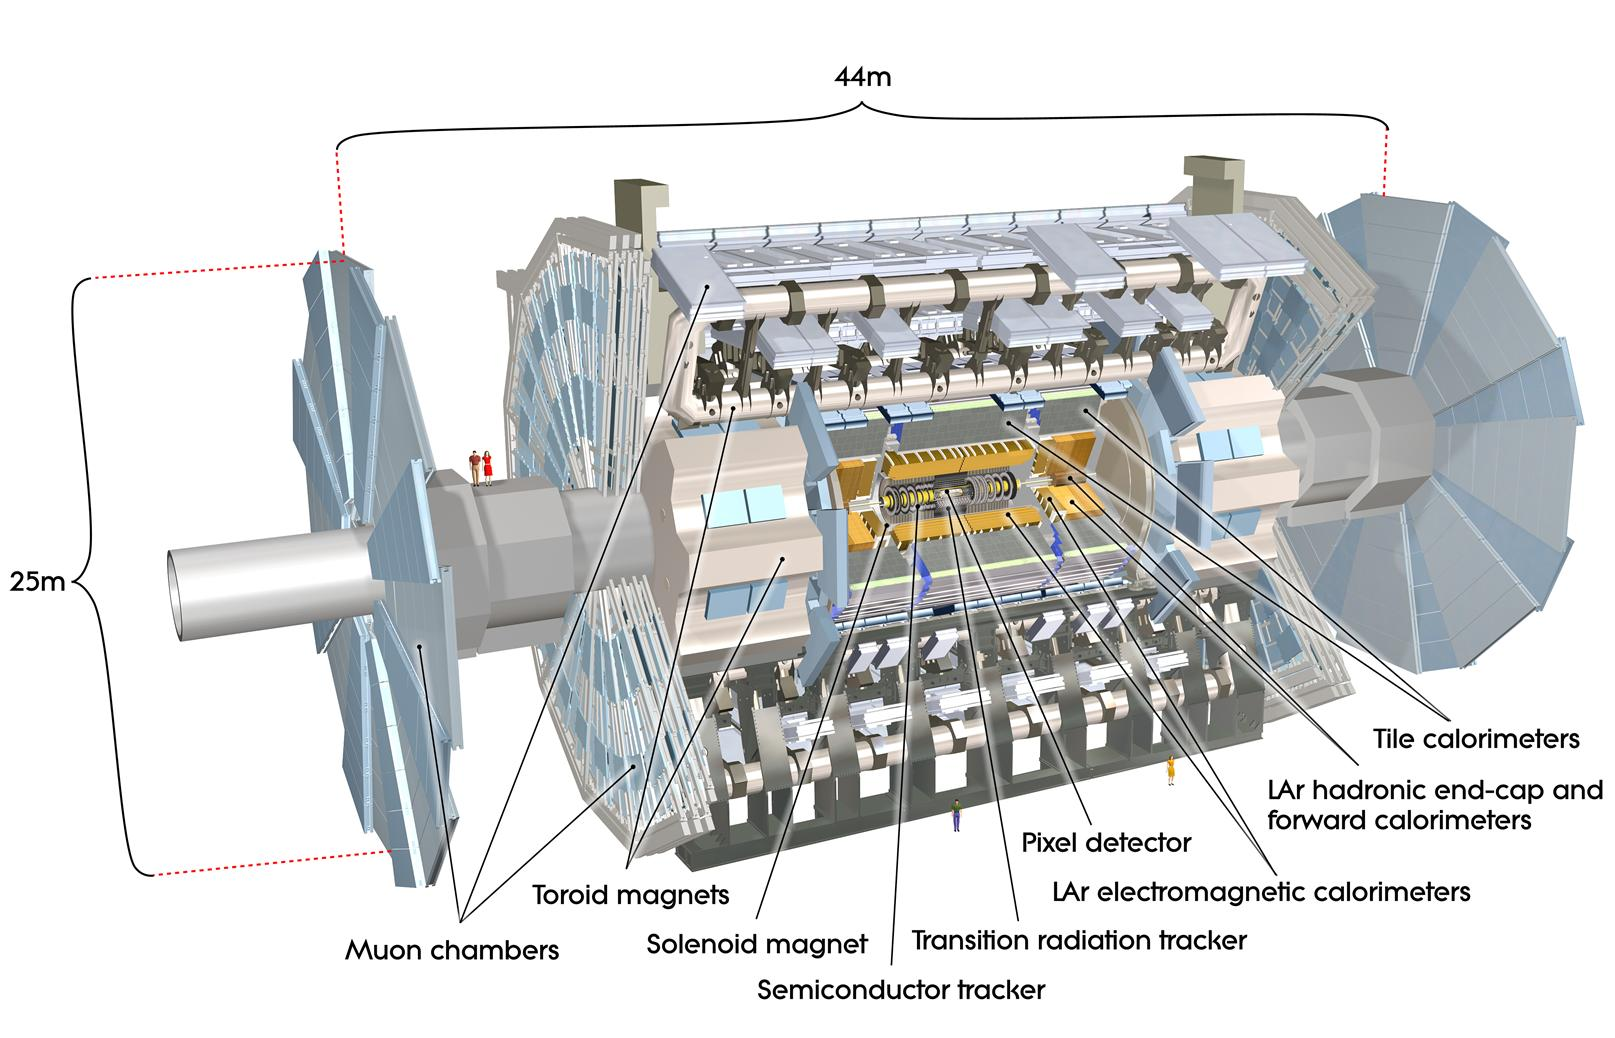
\includegraphics[width=0.9\textwidth]{detector/figures/atlas}}
	\caption{Schematic drawing of the ATLAS experiment. The detector subsystem are indicated as well as the total dimensions.\label{fig:atlas}}
\end{center}\end{figure}

\begin{figure}[htb]\begin{center}
	\subfigure{
  	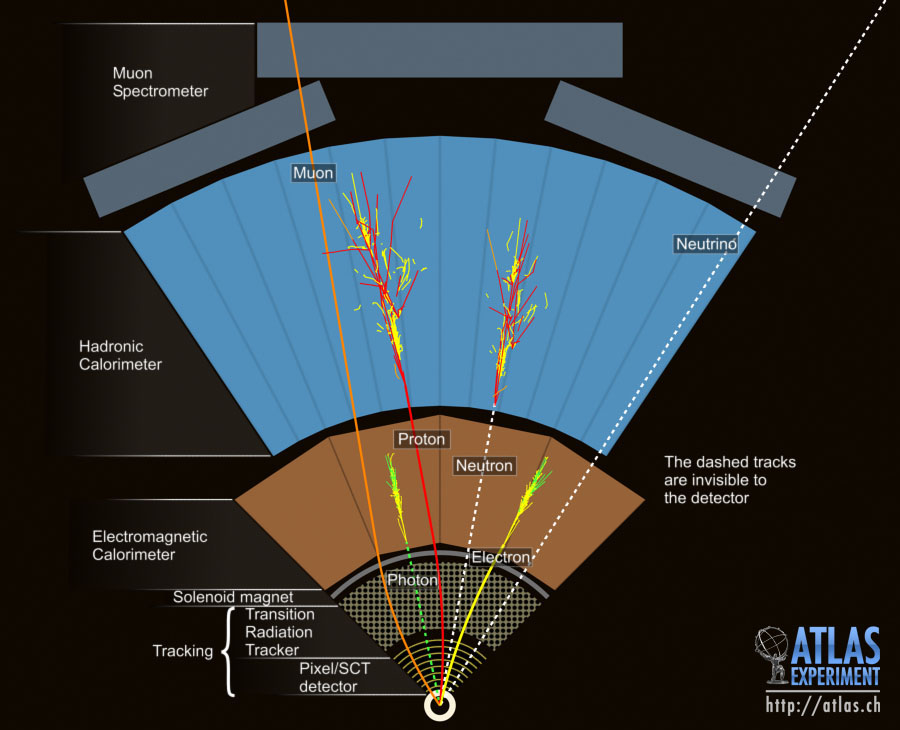
\includegraphics[width=0.75\textwidth]{detector/figures/detection}}
	\caption{Drawing of the detection of particles going from the interaction point through the whole detector.\label{fig:detection}}
\end{center}\end{figure}


\subsection{Coordinate system}

Protons from the two circulating beams are made to collide in the center of the ATLAS detector, in the region
that takes the name of Interaction Point (IP). The IP is taken as the origin of a three dimensional XYZ right-handed
coordinate system. The Z axis is tangent to the trajectory of the beams while the XY plane is perpendicular to
it and defines a symmetry plane for the detector, dividing it into the $A$ and $C$ sectors, respectively in the
positive and negative Z semi-axes. Figure~\ref{fig:coord} shows a schematic of the coordinate system.

\begin{figure}[tb]\begin{center}
	\subfigure[]{\label{fig:coord}
  	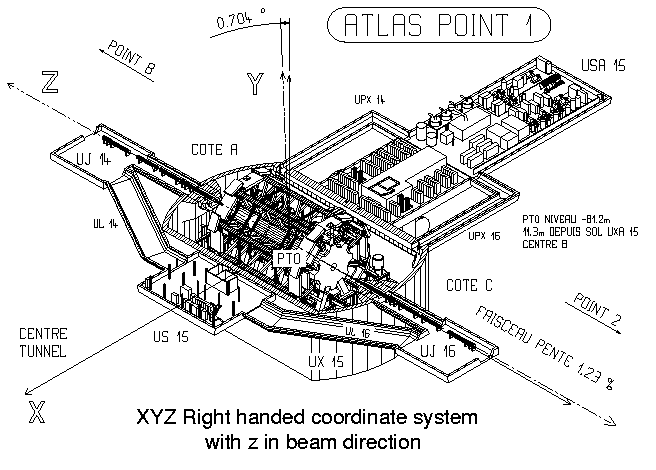
\includegraphics[width=0.6\textwidth]{detector/figures/coord}}\hskip3ex
        \subfigure[]{\label{fig:spherical}
  	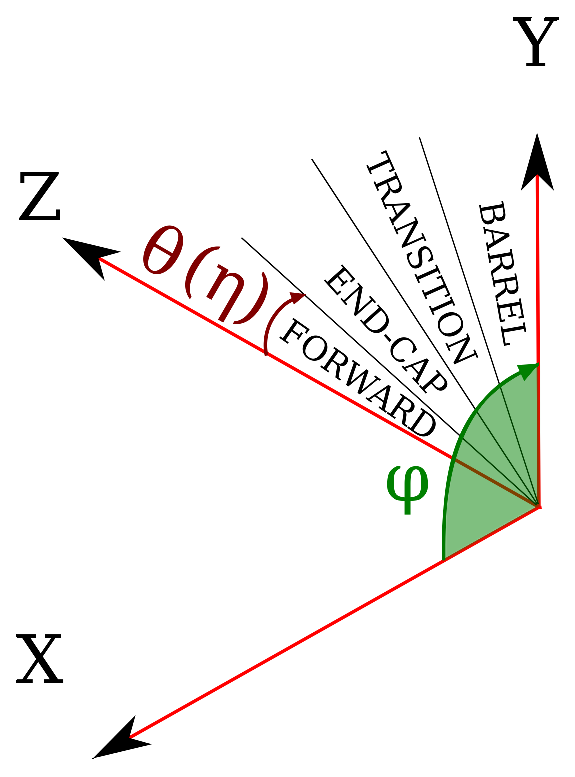
\includegraphics[width=0.3\textwidth]{detector/figures/spherical}}
	\caption{(a) Drawing of the ATLAS experiment with the cartesian coordinate system. The positive X axis points towards the center of the LHC
        ring. The positive Z axis points todards the anti-clockwise circulating direction of beam 2. (b) Simple schematic showing the spherical coordinates and the
        region definition in terms of the absolute value of the pseudorapidity $\eta$. These regions are symmetrical with respect to the transverse
        XY plane.}
\end{center}\end{figure}

In terms of polar coordinates, the Z axis is again along the beam axis and in the transverse plane 
the $R$ and $\phi$ coordinates are defined with $\phi$ ranging between 
$-\pi$ and $+\pi$ with respect to the X axis. In terms or spherical coordinates (see Figure~\ref{fig:spherical}),
the radial vector $R$ originates from the IP,  the azimuth $\phi$
is the same as the polar angle $\phi$, 
and the polar angle $\theta$ is measured with respect to the Z axis and
ranges between 0 and $\pi$. 

Since the interaction initial energy is unknown, being dependent on the parton distribution functions for the proton
energy, it is useful to define the transverse component of variables of 
interest\footnote{These quantities transverse initial value will be, indeed, zero, as the protons are accelerated along the Z axis.}  
like the energy and the momentum, being taken as the projection on the XY plane:

\begin{equation}\label{eq:transv}
\et = E\sin\theta, \qquad \pt = p\sin\theta.
	\end{equation}

Another common variable used at hadron colliders to describe the polar distribution and preferred to the simple
polar angle $\theta$ is the pseudorapidity $\eta$:
\begin{equation}\label{eq:pseudorapidity}
        \eta \equiv -\ln\bigg(\tan\frac{\theta}{2}\bigg);
	\end{equation}
which, for relativistic regimes, is equal to the rapidity $y$:
\begin{equation}\label{eq:rapidity}
y \equiv \frac{1}{2} \ln \bigg(\frac{E+p_{Z}}{E-p_{Z}}\bigg);
	\end{equation}
and $\Delta y$ and $\Delta \eta$ are Lorentz invariant. The pseudorapidity is preferred
to the rapidity as it does not require knowing the particle mass but only its polar position.
The distance between two particles is often referred to in terms of $\Delta R$:
\begin{equation}\label{eq:deltar}
\Delta R = \sqrt{(\Delta\eta)^{2} + (\Delta\phi)^{2}}.
	\end{equation}


%since particles produced in collisions are not uniformely distributed in $\theta$. 
Figure~\ref{fig:spherical} shows how different pseudorapidity regions are named. Particles
along the Z axis have a pseudorapidity $|\eta|=\infty$, particles along the Y axis have
a pseudorapidity $|\eta|=0$. ATLAS has an excellent hermeticity and is able to cover 
pseudorapity regions up to $|\eta|=4.9$. Typically, physics analysis consider objects in
the pseudorapity region  $|\eta|<2.5$. For a quick visualization of the correspondence
in terms of polar angle distribution, some pseudorapidity values are reported in Table~\ref{tab:etatheta}.
%AAAAAAAAAAAAAAAAA add barrel forward blabla exact def


\begin{table}[htb]\centering\begin{tabular}{cccccccccc}\toprule
$\theta$ & 0$^{\circ}$ & 5$^{\circ}$ & 10$^{\circ}$ & 20$^{\circ}$ & 30$^{\circ}$ & 45$^{\circ}$ & 60$^{\circ}$ & 80$^{\circ}$ & 90$^{\circ}$ \\
$\eta$ & $\infty$ & 3.13 & 2.44 & 1.74 & 1.31 & 0.88 & 0.55 & 0.175 & 0\\\bottomrule \end{tabular}
\caption{Pseudorapidity vs polar angle values.}\label{tab:etatheta}\end{table}

\subsection{Magnets}\label{sec:magnets}

ATLAS is provided with four superconducting magnets that allow the measurement of
charged particles momenta by curving their trajectory. 

A central solenoid, 5.3~m long and 2.4~m in diameter, sits 
around the inner detector and produces a 2~T magnetic field along the direction
parallel to the beam axis. It is only 45~mm thick (equivalent to 0.66 radiation lenghts $X_0$)
and is cooled with liquid Helium, sharing the cryostat with the electromagnetic calorimeter.

Paired to the muon spectrometer, the superconducting air-core toroid magnet (Figure~\ref{magnets}) 
has an open structure with eight superconducting toroidal coils in the barrel part (each 25.3~m long, located
at the outer diameter of 20.1~m) and
two end-cap systems made of eight coils. The field strength varies strongly with $\phi$:
in the barrel region ($|\eta|<1.4$) is 1.5-5.5 Tesla$\cdot$m; in the end-caps ($1.6<|\eta|<2.7$) 1-7.5 is Tesla$\cdot$m. 
Such configuration of the magnets gives a field orthogonal to the muons trajectory.

\begin{figure}[hbt]\begin{center}
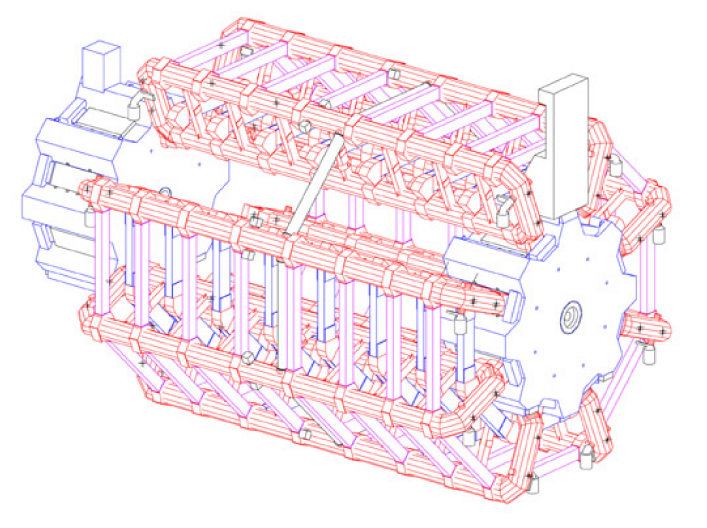
\includegraphics[width=.8\textwidth]{detector/figures/magnets}\caption{Toroidal magnet system.}\label{magnets}
\end{center}\end{figure}



\subsection{Inner detector}\label{sec:innerdet}

The Inner Detector (ID) is the subsystem closest to the IP and tracking charged particles arising from collisions allows for 
the measurement of their momentum and vertex reconstruction with excellent resolution. At the design choices level, radiation resistance had to
be taken into account, as well as reducing the amount of material to be placed in front of the calorimeters to avoid spoiling the energy measurement.
This quantity varies between 0.5 and 2.5~$X_0$ depending on the pseudorapidity region, most of it coming from supporting equipment. This material
is responsible for photon conversions and electron bremsstrahlung.

The ID is surrounded by the central solenoid magnet (Section~\ref{sec:magnets}) and is composed by three subsystems, 
from the closest to the furthest from the IP: the pixel detector, the SemiConductor Tracker (SCT) and
the Transition Radiation Tracker (TRT).
%silicon strip detector and a straw detector (Figures~\ref{fig:innerdet1} and~\ref{fig:innerdet2}).

\begin{figure}[tb]\begin{center}
	\subfigure[]{\label{fig:innerdet1}
  	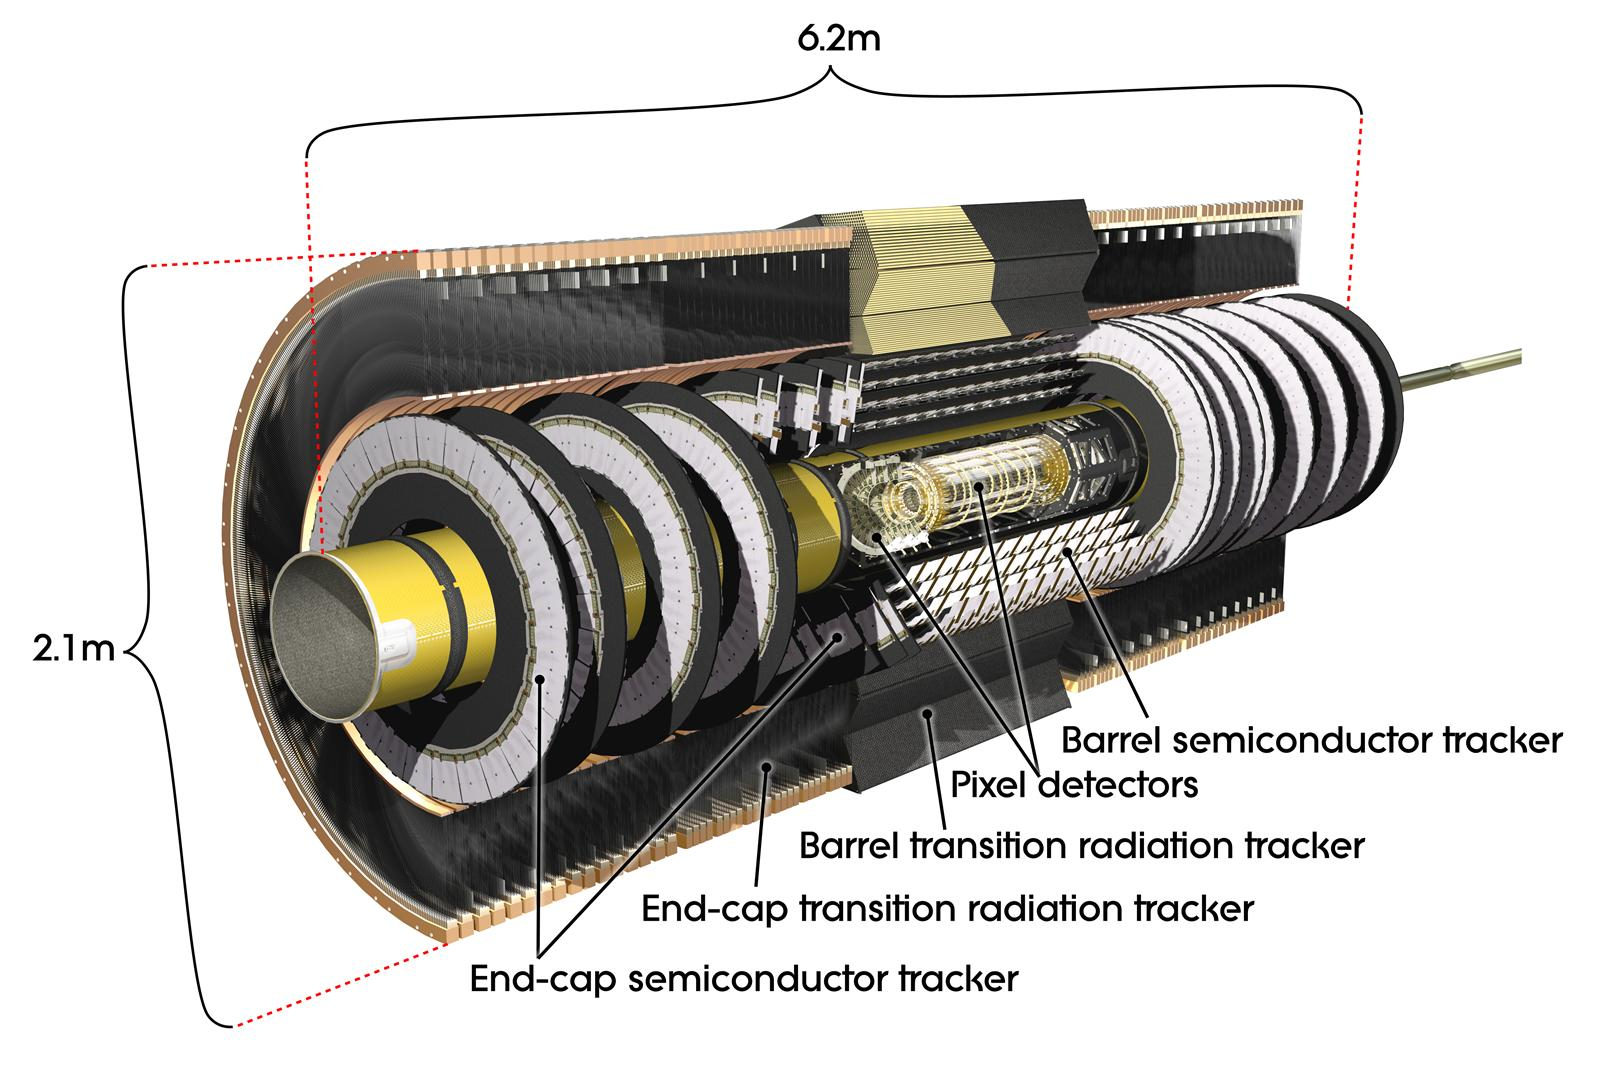
\includegraphics[width=0.6\textwidth]{detector/figures/innerdet}}
	\subfigure[]{\label{fig:innerdet2}
  	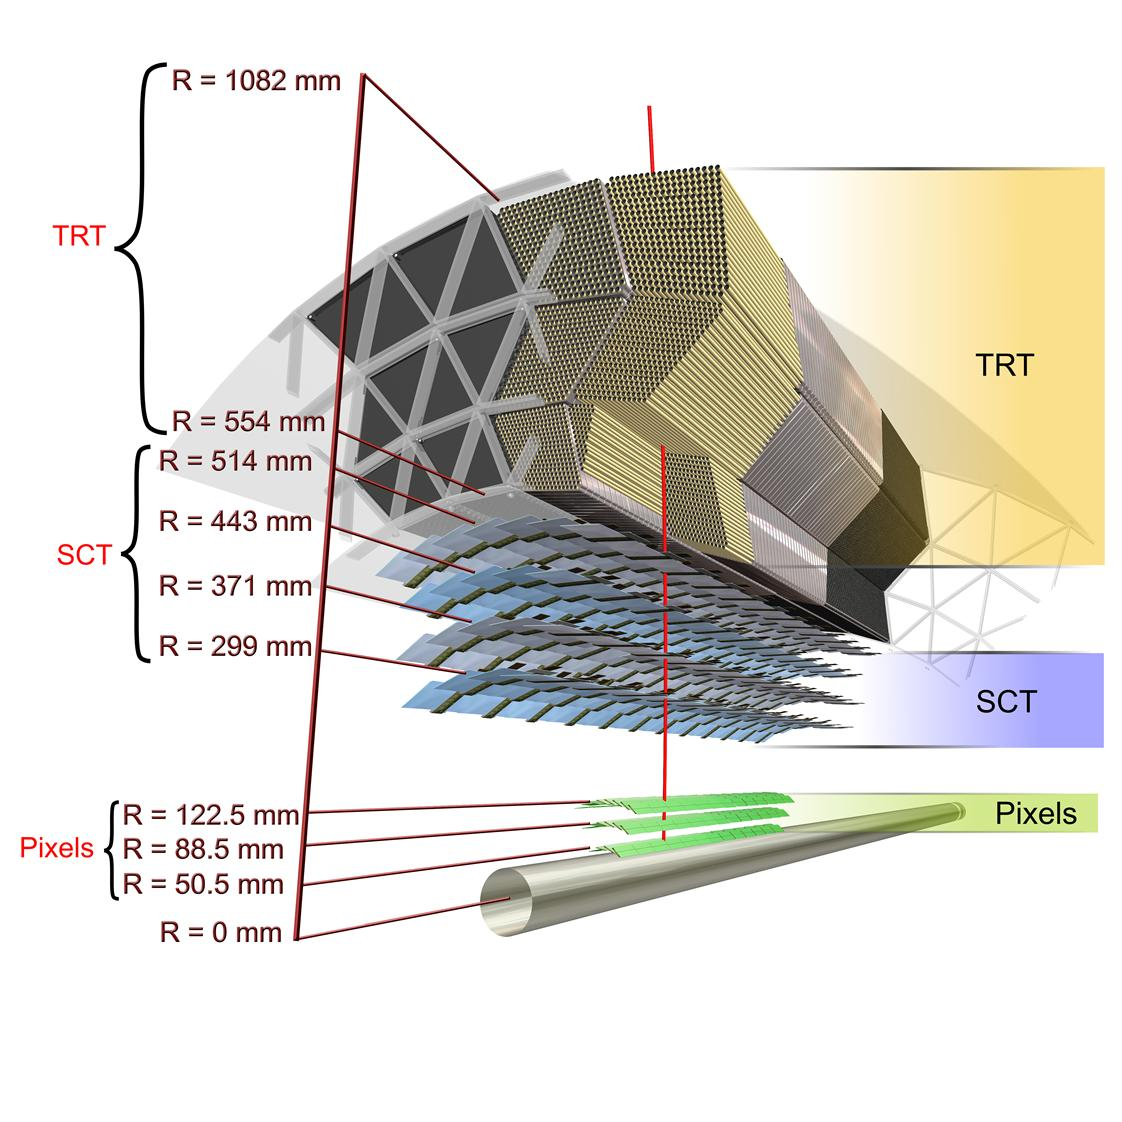
\includegraphics[width=0.37\textwidth]{detector/figures/innerSection}}
	\caption{(a) Schematic of the ID system. (b) Detailed schematic of the barrel section of the ID showing the
        three subsystems and reporting the distance to the center of the beam pipe.}
\end{center}\end{figure}


\subsubsection{Pixel detector}

The first subsystem covers the region $|\eta|<2.5$ and  is composed by three cylindrical layers in the barrel region, each of them distant from the beam by
50.5~mm, 88.5~mm and 122.5~mm respectively, and by three concentric discs in the end-cap region, each of them distant from the beam by
49.5~mm, 58.0~mm and 65.0~mm respectively.
Each silicon pixel has a size of 50$\times$400~$\mu$m$^{2}$ and is 250~$\mu$m thick, 
with in total $\sim$80.4 million readout channels to achieve a very fine granularity.
The precision is of 10~$\mu$m in $R\phi$ and 115~$\mu$m in Z and $R$ in the barrel and end-cap
region respectively.

The very first layer is called $B-$layer as, thanks to its position really close to the IP,
allows for the reconstruction of secondary vertices associated with the production of
 short lived particles such as $B-$hadrons. This information is very useful to identify
jets originating from the fragmentation of $b$ quarks.

\subsubsection{Semiconductor tracker}

After the three layers of pixel detectors, come four layers of  silicon strip detectors. The SemiConductor
Tracker (SCT) also covers the region $|\eta|<2.5$ with a barrel and end-cap design similar to the 
pixel detector one, being composed by eight silicon strips (two per layer) 128~mm long and 80~$\mu$m large.
It makes use of $\sim$6.3 millions readout channels and the resolution achieved is of 17~$\mu$m 
in $R\phi$  and 580~$\mu$m in Z ($R$) in the barrel (end-cap) region.

By allowing for four redundant position measurements\footnote{One of the coupled layers is rotated of $40$mrad with respect
to the other, which is parallel to the axis, giving a small stereo angle for a redundancy in the $\phi$ coordinate measurement.}, 
the SCT contributes mainly to the momentum reconstruction.

%Silicon has a band gap of just 3.6 eV, that is the minimum energy to create an electron/hole pair. Thus a minimum ionising particle creates around 80 electron/hole pairs per $\mu$m through primary and secondary ionisation.

\subsubsection{Transition Radiation Tracker}

In order to reduce the amount of material in front of the calorimeters, and to reduce the construction costs as well,
in the third subsystem the semiconductor technology has been substituted with straw detectors.
The Transition Radiation Tracker (TRT) consists of thin proportional chambers made of straw polyimide drift tubes, 4~mm in diameter.
The drift tubes are filled with a gas mixture composed of: 70\% Xenon, 27\% Carbon Dyoxide, 3\% Oxygen. The anode 
collecting the electrons from the ionized gas at the passage of the charged particle is made of
tungsten covered in gold.

In the barrel region the tubes are 144~cm long and placed parallel to the beam axis, while in the 
end-cap region they are 37~cm long and positioned radially in wheels, with layers of radiator foils alternated 
to layers of straws. The resolution achieved is of 130~$\mu$m in $R\phi$ and Z$\phi$  in the two regions respectively.
The covered pseudorapidity region is of $|\eta|<2.0$ and the readout is composed by $\sim$351000 channels.

About 36 measurements per track are taken, and since each channel provides two independent thresholds per hit,
it is possible to discriminate between electrons and pions, since the former will more likely reach the
high threshold.

In the end, the combination of the three ID subsystems gives very precise $R\phi$ and Z measurements, as well as good track pattern recognition.
The resolution on the transverse momentum, measured with cosmic muon calibration runs~\cite{id_cosmic}, is:

\begin{equation}\label{eq:momentumres}
\frac{\sigma_{\pt}}{\pt}=P_1 \oplus P_2 \times \pt,
	\end{equation}
where $P_1=1.6\pm0.1\%$ and $P_2=(53\pm2)\times10^{-5}$~\GeV$^{-1}$. This means a 
resolution of~$\sim$1.6\% for tracks with $\pt\sim$1~\GeV\ and 
$\sim$50\% for tracks with $\pt\sim$1~\tev.


\subsection{Calorimeters}\label{sec:calo}

Particles leaving the ID and surviving the crossing of the central solenoid magnet
will face the calorimeter system, depicted in Figure~\ref{fig:calorimeters}.
The full system is characterized by a coverage
in pseudorapidity up to $|\eta|<5$ and an almost full coverage in $\phi$. With its 
22~$X_0$ and 24~$X_0$ radiation lengths of material in the barrel and end-cap regions respectively 
it is also able to stop most of the non-muon particles from the interaction.
Besides particles energy measurement, the calorimeters provide particle identification
information, discriminating electrons, photons and jets, and the determination
of the missing transverse energy.

Different technologies are used in the barrel, end-cap and forward regions for both the
electromagnetic and the hadronic calorimeters. All of them are sampling calorimeters,
with a dense medium acting as absorber to stop particles and start showers, and an
active material to detect the signal from ionization. For the electromagnetic calorimeters
and the forward hadronic calorimeter liquid argon is used as active medium, while the
barrel and extended-barrel hadronic calorimeter uses scintillating tiles.
The liquid argon is cooled at a temperature of about 88~K, with the use of two sets of cryostats:
the barrel electromagnetic calorimeter shares the cryostat with the central solenoid;
the end-cap and forward electromagnetic calorimeter and the hadronic end-cap calorimeter
share a cryostat in the foward region.

\begin{figure}[tb]\begin{center}
	\subfigure{
  	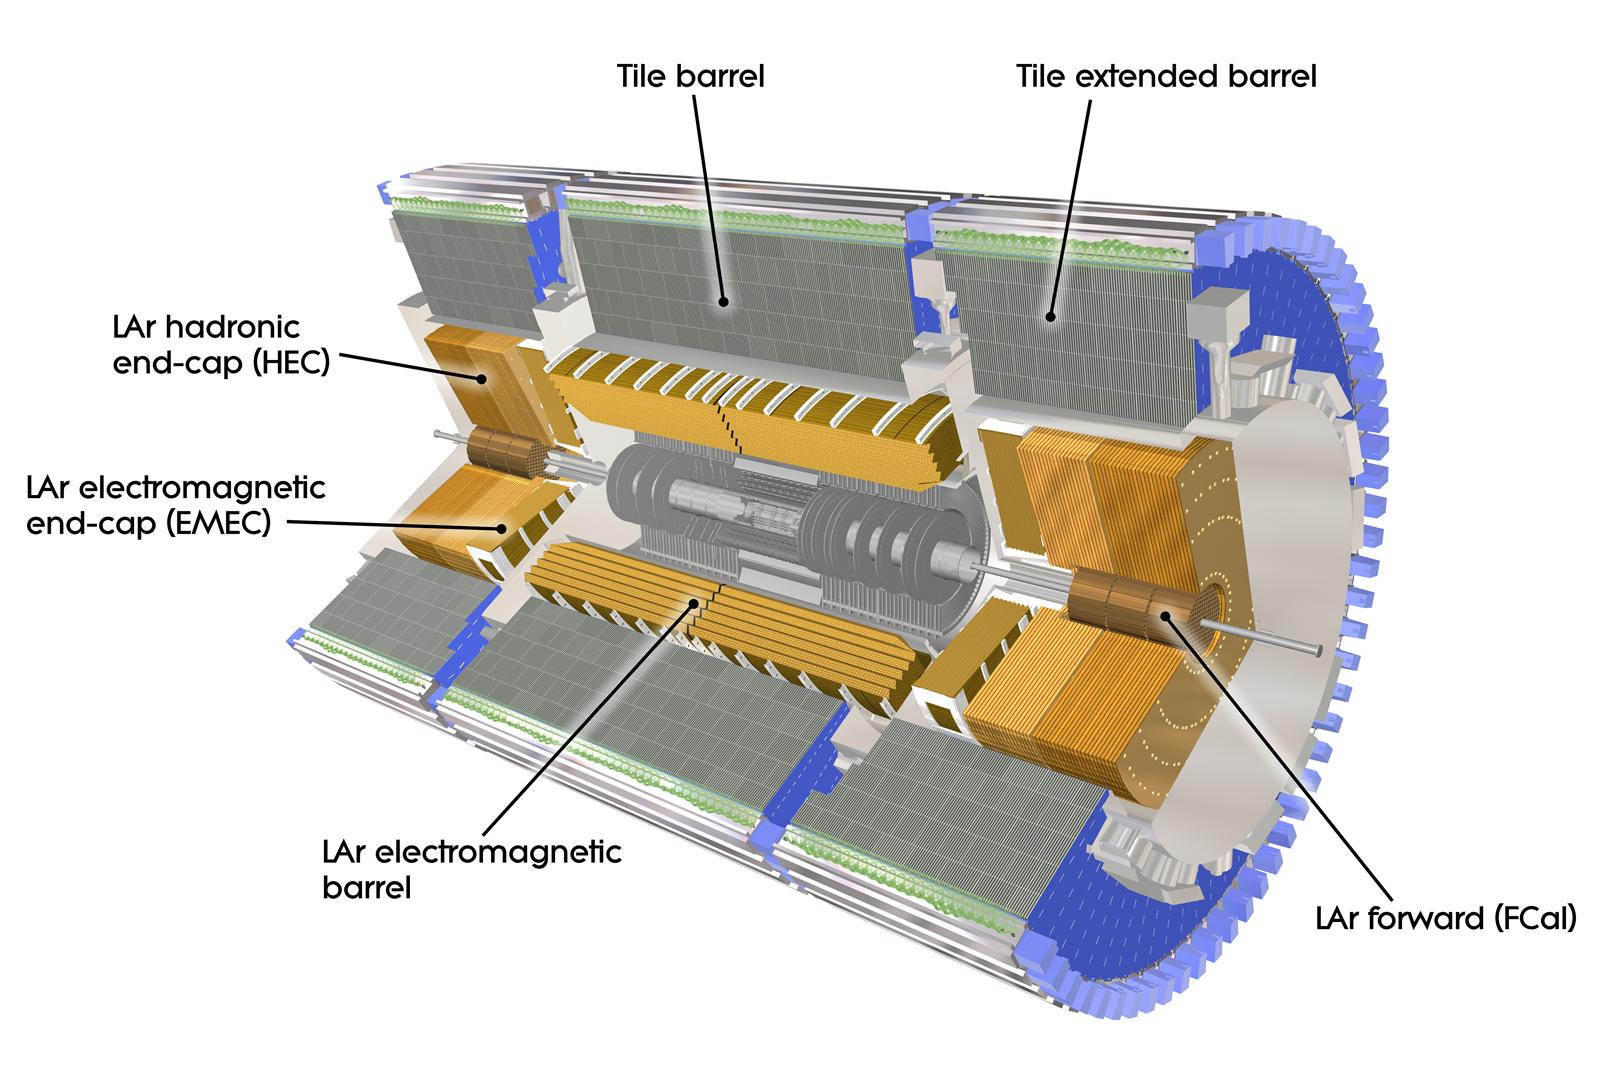
\includegraphics[width=0.8\textwidth]{detector/figures/caloBarrel}}
	\caption{Schematic of the calorimeter complex of the ATLAS detector.\label{fig:calorimeters}}
\end{center}\end{figure}

Particles interact both with the passive and active material, but only the energy released
in the active samples will be detected. 
%The balance, chosen at the design stage, between
%the two elements will determine how much the calorimenter compensate for the 
The processes involved in the shower formation are several and mainly electromagnetic.
Photons in matter can undergo the photoelectric effect, Compton scattering and $\gamma \to \epem$
pair formation. The general contribution of these processes depends both on the photon energy
and on the atomic number $Z$ of the material, and is shown in Figure~\ref{fig:photonsmatter}.
Electrons and positrons can ionize atoms and molecules, produce bremsstrahlung $\epm \to \epm + \gamma$
and emit Cerenkov radiation. Unless the calorimeter has been specifically designed for it,
 Cerenkov radiation does not contribute much, while ionization is the main process for energies
up to $\sim 100$~\mev, where bremsstrahlung starts to dominate.

In general, these cascade of events
continues until a certain threshold is reached, and the final number of particles
produced is proportional to the energy of the first particle originating the shower.

\begin{figure}[tb]\begin{center}
	\subfigure{
  	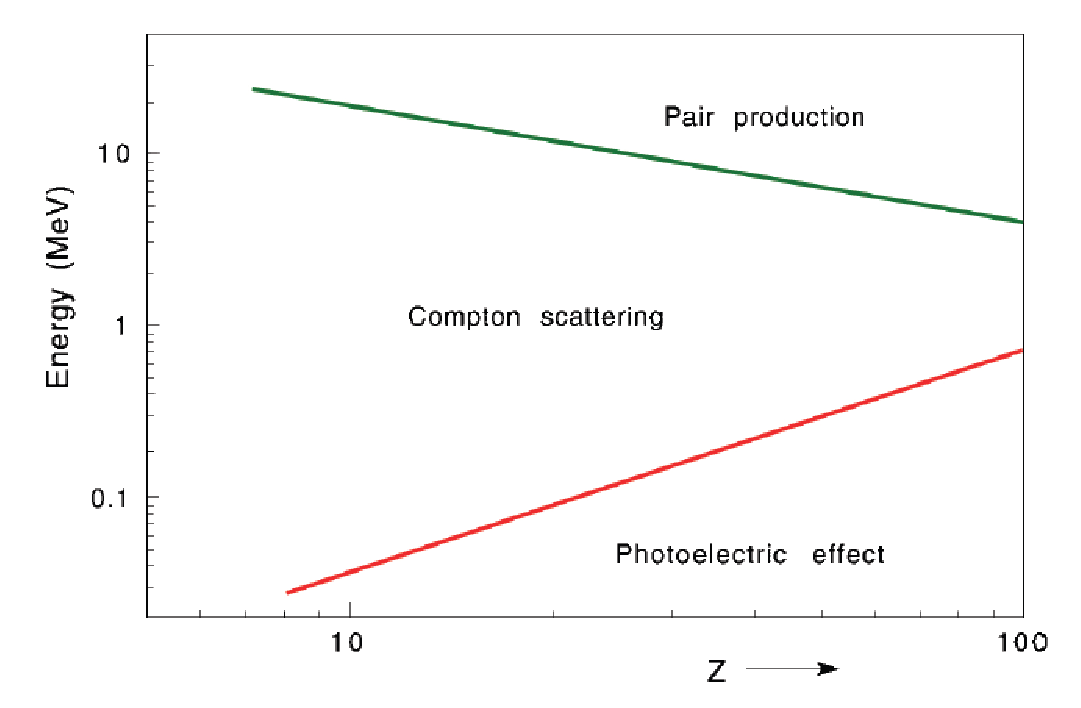
\includegraphics[width=0.6\textwidth]{detector/figures/photonsmatter}}
	\caption{Domains in term of photon energy and $Z$ number of the absorber material
        in which photoelectric effect, Compton scattering and pair production are the 
        favorite processes for energy loss~\cite{Wigmans}.\label{fig:photonsmatter}}
\end{center}\end{figure}

Also hadrons interact with matter, either ionizing it (if charged) or by nuclear interactions.
The problem of the latter process is that this energy release is often not directly detectable,
like in nuclear breakups and excitations, and is therefore called ``invisible energy''.
Secondary hadrons will be produced, forming the hadronic part of the shower, but sooner
or later something like $\pi^0\to \gamma\gamma$ will happen and the shower will
develop electromagnetically further on.

The average fraction of electromagnetic and hadronic shower components is a characteristic
of the sampling calorimeter and depends on the choice of the passive and active material
and on the design. Calorimeters are said to be {\it non-compensating} if, like the ATLAS
calorimeters, the detection of hadronic showers is less efficient than the one of 
electromagnetic showers. Calorimeters with a similar response for the two components
are called  {\it compensating}, while calorimeters more efficient when revealing
hadronic showers are  {\it over-compensating}.

%The distinction between electromagnetic and hadronic calorimeters is due to the different phenomenology of the physics involved. The development of electromagnetic showers from an incident electron or photon is well understood and for particles with equal incident energy the variations in shape and measured energy of the showers are quite small. The size of the shower is linearly dependent on the radiation length $X_{0}$ of the material entered, while the size of hadronic showers depends linearly on the nuclear interaction length\footnote{The nuclear interaction length is the average distance traveled by hadrons before inducing a nuclear reaction.} $\lambda_{int}$ of the material. 

The performance for the energy resolution is parametrized by the following formula:
\begin{equation}\label{eq:resolution}
\frac{\sigma_{E}}{E} = \frac{S}{\sqrt{E}}\oplus\frac{N}{E}\oplus C,
\end{equation} 
where the terms of the sum correspond, respectively, to a ``stocastic'' term related to how shower develops in the sampling calorimeter; to a ``noise''
term including the contribution from electronic noise and pile-up energy fluctuation; 
to a systematic term that depends on calibration, shower containment, inactive material and on the
linearity of the response as well. 

The goal energy resolution for the liquid argon calorimeters is~\cite{lar_readiness}:
\begin{equation}
\frac{\sigma_{E}}{E}=\frac{10\%}{\sqrt{E}} \oplus\frac{170\MeV}{E} \oplus 0.7\%,
\end{equation}
while for the hadronic barrel calorimeter is~\cite{tile_readiness}:
\begin{equation}
\frac{\sigma_{E}}{E}=\frac{50\%}{\sqrt{E}} \oplus 5\%.
\end{equation}
Test-beam runs to measure the response of the two calorimeters to electrons
and single pions respectively have shown results comparable to the goal resolutions.


\subsubsection{Electromagnetic calorimeter}\label{sec:emcalbarrel}

The electromagnetic calorimeter, also called LAr calorimeter (from Liquid Argon, the active material),
can measure electrons and photons energies in the range from 50~\mev\ to 3~\tev.
In the barrel region it is referred to as EMB (ElectroMagnetic Barrel), is 
divided into two identical semi-barrels EMBA and EMBC separated at Z=0 by a 6~mm
gap and covers the pseudorapidity region $|\eta|<1.475$. 
Two end-cap detectors (EMEC, ElectroMagnetic End-Cap), divided 
into two coaxial wheels, cover the pseudorapidity 
regions $1.375<|\eta|<3.2$. A pre-sampler, extended over 
$|\eta|<1.8$, stands in front of the EMB and allows for the measurement of
the energy the particles lost before reaching the EMB i.e. crossing the
material of the ID, the central solenoid and the cryostat.

Three longitudinal samples in the EMB are designed for different tasks. The first
sample, 4.3$X_0$ long, is finely segmented in $\eta$ to precisely measure
the direction in pseudorapidity of the particles with  thin readout strips
of $\Delta\eta\times\Delta\phi$ = 0.0031$\times$0.098. This helps for
photon/$\pi^{0}$ discrimination and as well for separate close-by $\gamma$s
from $\pi^{0}$ decay.
The second sample, 16$X_0$ long, contains the bulk of electrons and photons energy deposit. 
It is divided in towers with dimension $\Delta\eta\times\Delta\phi$ = 0.025$\times$0.0245
and provides the position measurement of the cluster. 
The  95\% of the energy of the shower is deposited in a matrix of 3$\times$7 
towers $\Delta\eta\times\Delta\phi$.
The third sample, 2$X_0$ long, is coarsely segmentes and collects the last bit of the longitudinal
development of the electromagnetic showers. Towers in this region have a dimension
of $\Delta\eta\times\Delta\phi$ = 0.05$\times$0.0245.

Also the EMEC is divided in three longitudinal samples (two in the region $1.375<|\eta|<1.5$),
and besides the lead, also the thickness of the liquid argon layers are varied in the
radial direction.

\begin{figure}[tb]\begin{center}
	\subfigure[]{\label{fig:calolar}
  	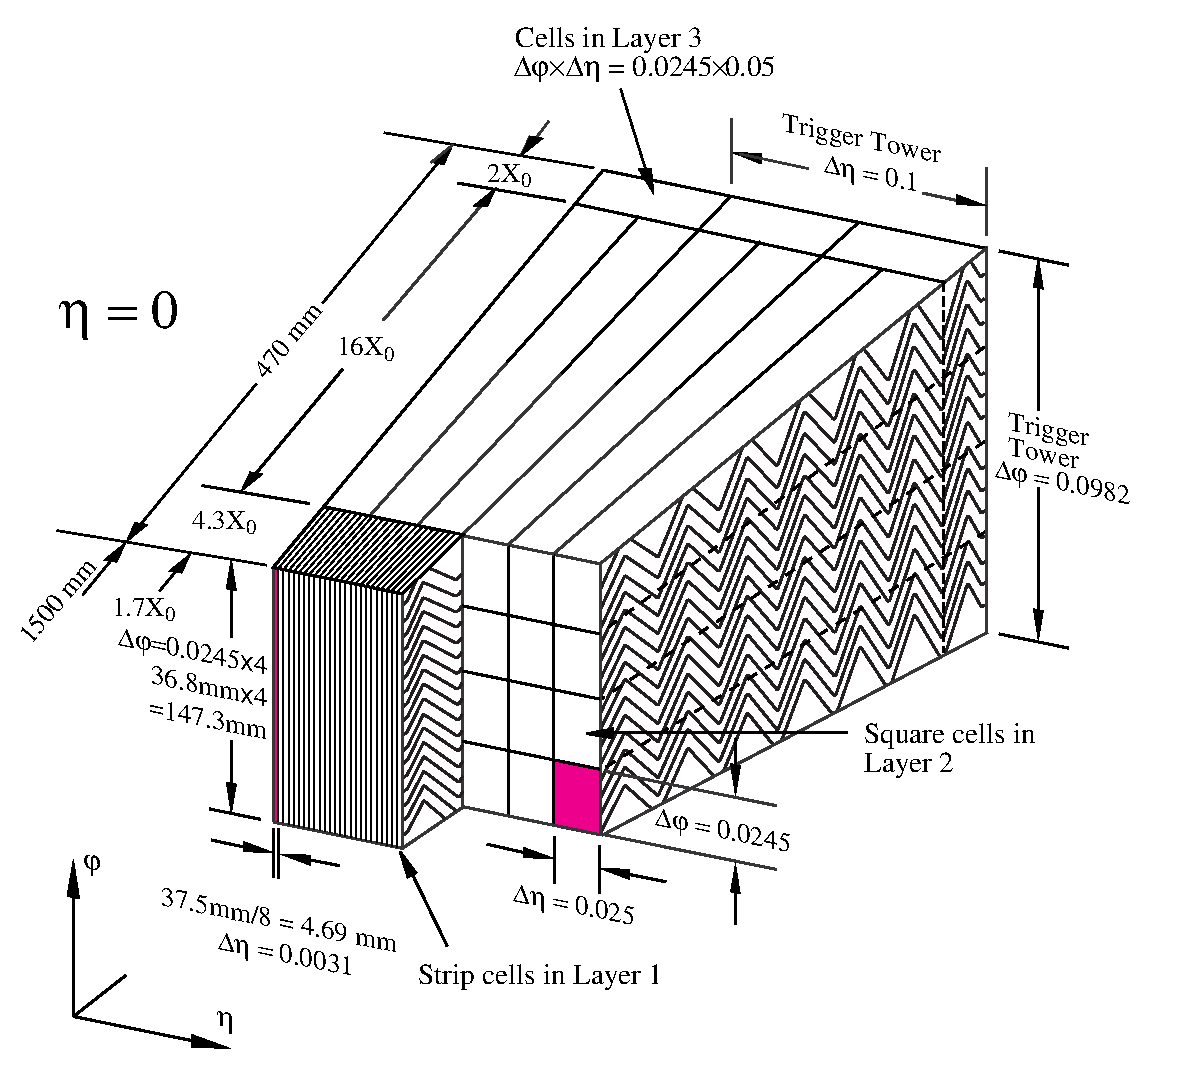
\includegraphics[width=0.48\textwidth]{detector/figures/caloLAr2}}
	\subfigure[]{\label{fig:calotile}
  	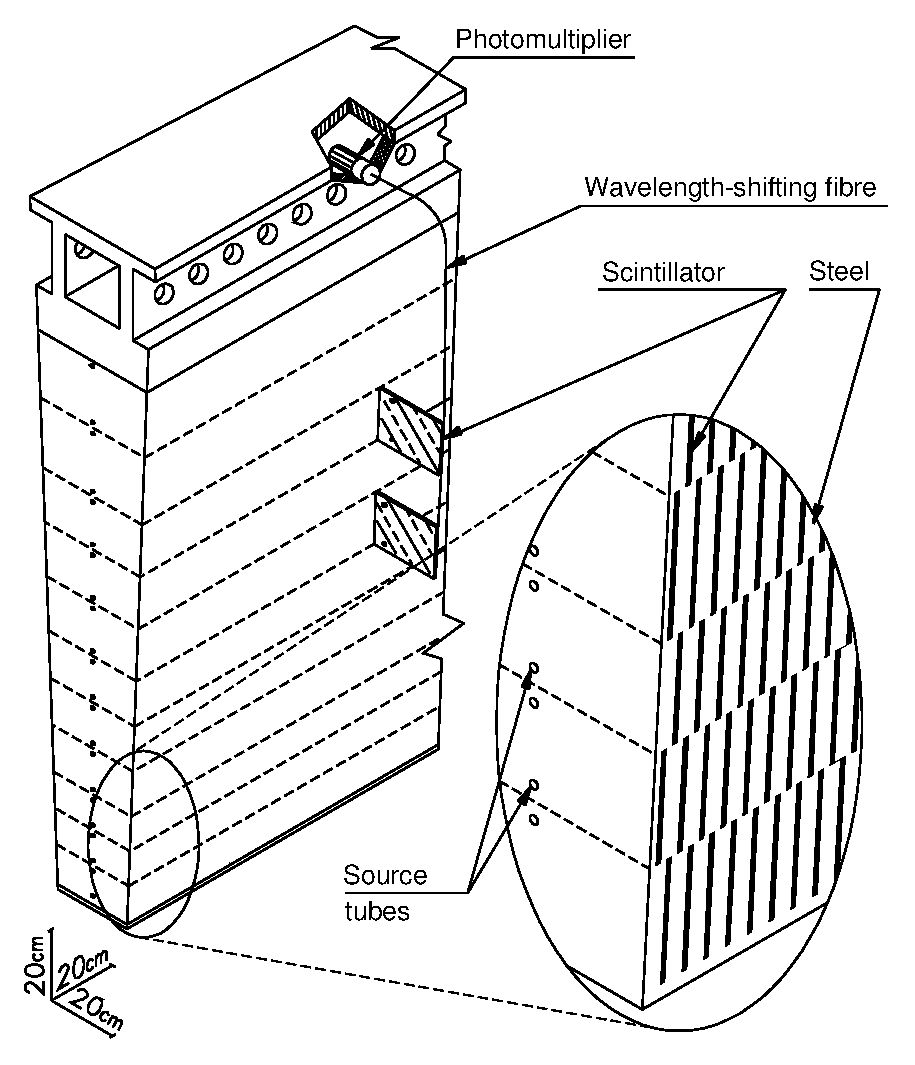
\includegraphics[width=0.38\textwidth]{detector/figures/caloTile}}
	\caption{(a) Schematic drawing of a module of the Electromagnetic barrel calorimeter. 
        (b) Schematic drawing of a module of the Hadronic barrel calorimeter.}
\end{center}\end{figure}


The absorbing material is lead shaped into an accordion geometry to achieve
full symmetry in $\phi$, as shown in the drawing of Figure~\ref{fig:calolar}.
Signal from the ionization produced in the liquid argon is collected
by an electrode in the middle of the active material region, fixed into
a honeycomb structure.

The thickness of the absorber layers depend on the pseudorapidity in
order to make particles entering the system with different incident 
angles cross the same amount of material.

\subsubsection{Hadronic calorimeters}\label{sec:hadcal}

Hadronic showers have typically a much longer shape than
electromagnetic ones, and need therefore in general more
interaction lenghts of material to be fully contained.
Hadronic calorimeters are therefore designed to completely
absorb high-energy hadrons, which will deposit only some (small) part of their energy 
in the electromagnetic calorimeter.



\subsubsection{Hadronic barrel calorimeter}\label{sec:hadcalbarrel}

The hadronic calorimeter in the barrel and extended barrel region, going up to
$|\eta|<1.7$, is made of scintillating tiles as active material with lead as absorber
and is commonly referred to with the name of TileCal. 
The light in the ultraviolet range that is generated in the tiles is collected through
wavelenght shifting optical fibre (Figure~\ref{fig:calotile}).

TileCal sits just after the electromagnetic
calorimeter and measures the energy and position of jets and isolated hadrons.
It is divided in depth in three layers with varying lenght (1.4, 4.1, 1.8 hadronic interaction
leghts $\lambda$ in the barrel and 1.5, 2.6, 3.3$\lambda$ in the extended barrel) and segmentation
($\Delta\eta\times\Delta\phi$ = 0.1$\times$0.1 in the first two layers,
$\Delta\eta\times\Delta\phi$ = 0.2$\times$0.1 in the third),
and in 64 slices in $\phi$, each of $\Delta\phi\sim0.1$.

The redout channels are grouped into cells that form a pseudo-projective geometry in $\eta$.

\subsubsection{Hadronic end-cap calorimeter}\label{sec:hadcalendcap}

The Hadronic End-Cap calorimeters (HEC) use copper as passive material and liquid
argon as active material, chosen for its radiation hardness in a region ($1.5<|\eta|<3.2$)
exposed to a significant amount of particle flux. Each HEC is composed by
two independent wheels with granularity varying with $\eta$: 
in $1.5<|\eta|<2.5$ $\Delta\eta\times\Delta\phi$ is 0.1$\times$0.1 in the first
two longitudinal layers,  0.2$\times$0.1 in the last one; in
$2.5<|\eta|<3.2$ $1.5<|\eta|<2.5$ $\Delta\eta\times\Delta\phi$ = 0.2$\times$0.2
in all the three samples.

The HECs collect the energy from particles that are not completely contained
in the EMECs and in particular are used to reconstruct jets and the missing transverse
energy.

\subsubsection{Forward calorimeter}\label{sec:calforward}

The Forward Calorimeter (FCal) cover the very forward region of pseudorapidity
$3.1<|\eta|<4.9$ making the calorimeter system achieve its good hermeticity
and minimize the energy losses.
It has an electromagnetic part that uses copper as absorber and two hadronic compartments
with tungsten as passive material. 




\subsection{Muon spectrometer}\label{sec:muonspec}

The most external detector system is the muon spectrometer, a combination
of toroidal superconducting magnets (Section~\ref{sec:magnets}) and precision
chambers providing a measurement of the momentum of muons in $|\eta|<2.7$ in addition
to the measurement from the ID. It is also equipped 
with an independent trigger system used for the first event triggering
stage (see Section~\ref{sec:lvl1}) active in the pseudorapidity region $|\eta|<2.4$. 

Four sub-detectors compose the muon system: Monitored Drift-Tube (MDT) chambers, 
Cathode Strips Chambers (CSC), Resistive Plate Chambers (RPC) and Thin Gap Chambers (TGC).
The layout changes in the barrel and end-cap regions, and is schematically shown in 
Figure~\ref{fig:muonSect}: in the  barrel region, chambers are arranged in three cylindrical layers around
the beam axis, one layer being inside the magnet; in the end-caps these three layers are placed 
perpendicular to the beam axis.

\begin{figure}[tb]\begin{center}
	\subfigure[]{\label{fig:muonSect2}
        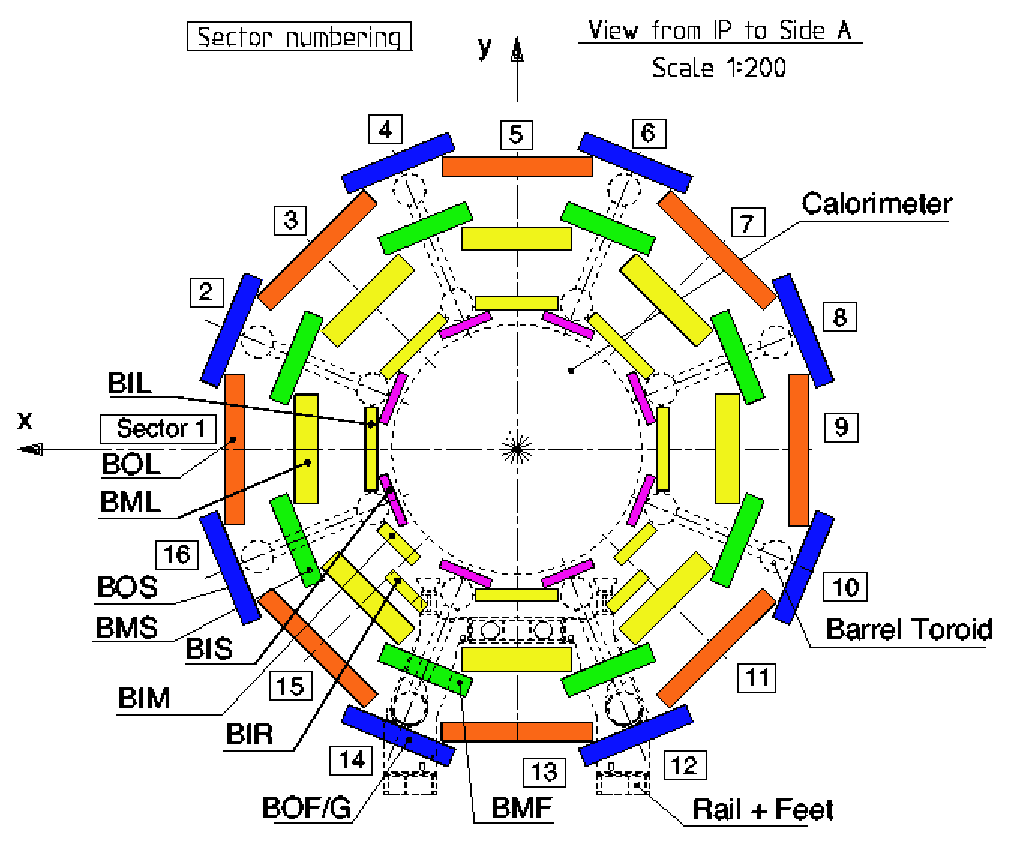
\includegraphics[width=.4\textwidth]{detector/figures/muonSect2}}
	\subfigure[]{\label{fig:muonSect}
        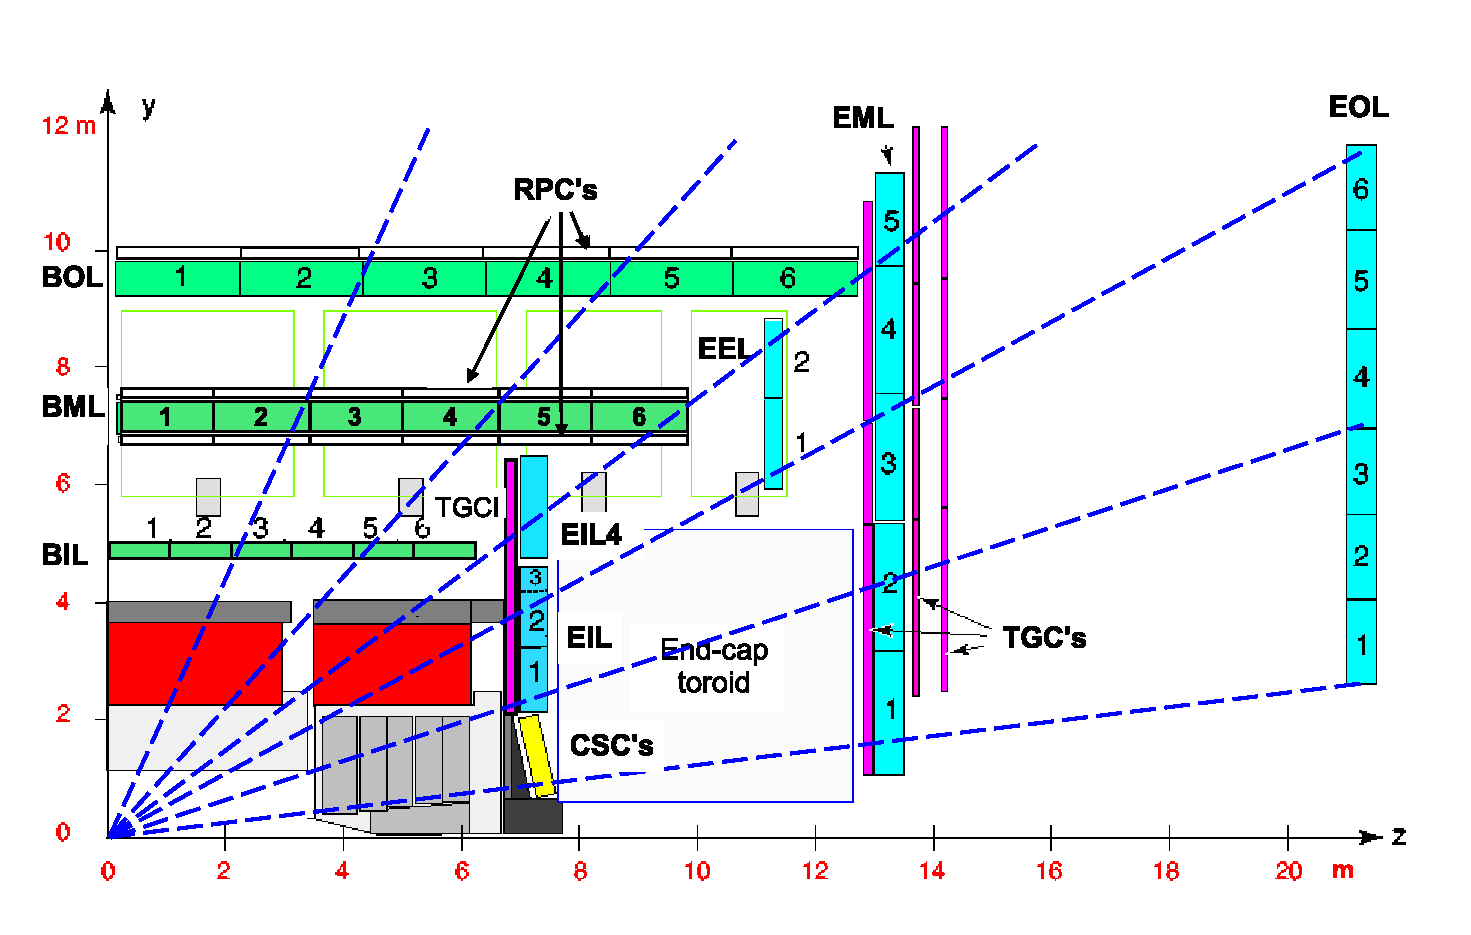
\includegraphics[width=.5\textwidth]{detector/figures/muonSect}}
	\caption{(a) Cross section of the barrel muon system. (b) Lateral section of the muon system. 
        Barrel MDTs are shown in green, end-caps MDTs in light blue, CSC in yellow, 
        TGCs in magenta, RPCs in white.%  (From \cite{Aad:JINST})
        }
\end{center}\end{figure}


\subsubsection{Detection chambers}

MDTs and CSCs are used to detect muons in the pseudorapidity regions $|\eta|<2.0$ and
$2.0<|\eta|<2.7$ respectively. MDTs are proportional chambers constituted by 
pressurised drift tubes made of aluminium with a diameter of 30~mm and lenght varying from 0.9~m to 6.2~m. 
The gas mixture in them is 93\% argon and 7\% carbon dioxyde, the anode is a 50~$\mu$m
tungsten-rhenium wire producing a radial electric field. Each chamber is composed by 
a group of six or eight tubes placed transverse to the beam axis. This number of tubes allows
for a very good track reconstruction and high reduction of the fake tracks from random 
associations of background hits, providing a resolution on position of 80 $\mu$m.
%gives a momentum  resolution $\sigma_{p_{T}}/p_{T} < 10^{-4}$~\GeV$^{-1} \cdot p_{T}$ for tracks with $p_{T} > $300~GeV.


The CSCs are used at higher $\eta$ to better cope with the higher particle flux.
They are arranged in a system of two disks with eight chambers each. Each chamber
contains four multiwire proportional chambers (the CSCs) with wires oriented in the radial direction,
spaced by 2.5~mm and in the same gas mixture of argon and carbon dioxyde as the MDTs.
The cathode strips are oriented one perpendicularly to the anode wires (and gives the precision coordinate)
and the other parallel to the wires (and gives the transverse coordinate).
The resolution provided by the interpolation between the charges induced on neighbouring cathode strips
ranges between 50 and 70 $\mu$m.

\subsubsection{Trigger chambers}

For trigger purposes detectors with faster response than drift tubes are needed\footnote{Drift-time in tubes with a diameter of 
$\mathcal{O}\sim 10$~mm can be of $\sim500$~ns, too long with respect to the 25 ns spacing of the bunch crossings.}.
MDTs and CSCs are then coupled with special layers of trigger chambers: in the barrel region, the MDT's second layer
is covered on both sides by RPCs, while MDT's third layer is covered by a RPC alternatively on the inner and outer side;
in the end–caps, TGCs cover the inner side of MDT's first and third layers. 

A RPC is a detector with a gas-gap between two resistive bakelite plates separated by 2~mm and containing
a gas mixture of C$_{2}$H$_{2}$F$_{4}$ (94.7\%), Iso-C$_{4}$H$_{10}$ (5\%) and SF$_{6}$ (0.3\%). 
RPCs measure six points per coordinate for each particle, quickly collecting the avalanches with two 
orthogonal sets of pick-up strips that provides a position resolution of 1 cm in each plane and 1 ns time resolution,
allowing for individual bunch crossing discrimination. Also RPCs provide the $\phi$ coordinate for the tracks in
the final analysis, since MDTs only give the $\eta$ coordinate.

TGCs are similar to CSCs, have 1.8~mm wire-to-wire separation and 
1.4~mm wire-to-cathode separation. They use a highly quenching gas mixture of CO$_{2}$ 55\% and n-C$_{5}$H$_{12}$ 45\%
and provide  a spatial resolution of about 1~mm and a time resolution of 5~ns.

\section{Forward sub-detectors}\label{sec:forward}

ATLAS is equipped with some detectors in the forward regions to perform additional measurements or
monitoring studies. In particular, the Minimum Bias Trigger Scintillators (MBTS), that are somehow
embedded in the structure of TileCal extended barrel modules (see Figure~\ref{fig:extendedbarrel})
and share with it the readout electronics, as they are also read by wavelenght-shifting fibers.
The MBTS consist of 32 scintillator paddles assembled in two disks covering the pseudorapidity region
$2.09<|\eta|<3.84$ and are used for trigger purposes to detect minimum bias activity during the first
runs of the LHC. 

MBTS are also used for relative luminosity measurements, but there are two detectors specifically
built to determine the luminosity delivered to ATLAS: LUCID and ALFA. LUCID (LUminosity measurements
using Cerenkov Integrating Detector) is made of 32 tubes surrounding the beam pipe 17~m
far from the interaction point on both sides of ATLAS and measures the luminosity bunch by bunch.
ALFA (Absolute Luminosity For ATLAS) is only activated during special runs, and consists of 8 
scintillating fibers detectors placed at 240~m from the interaction point inside roman pots, above and
below the beam pipe.

Another luminosity monitorer is the Zero-Degree Calorimeter, whose main purpose is to determine the centrality of heavy-ion
collisions. Placed at 140~m from the interaction point on both sides of the beam axis, is made of quartz rods
alternated with tungsten plates.

Finally, the Beam Condition Monitor (BCM) is made of two sets of diamond sensors located 184~cm close
to the interaction point along the beam and 5.5~cm close along $R$. Its task is to detect beam losses,
potentially harmful for ATLAS, and in that case to alert LHC in order to stop the accelerator.



\begin{figure}[tb]\begin{center}
	\subfigure{
  	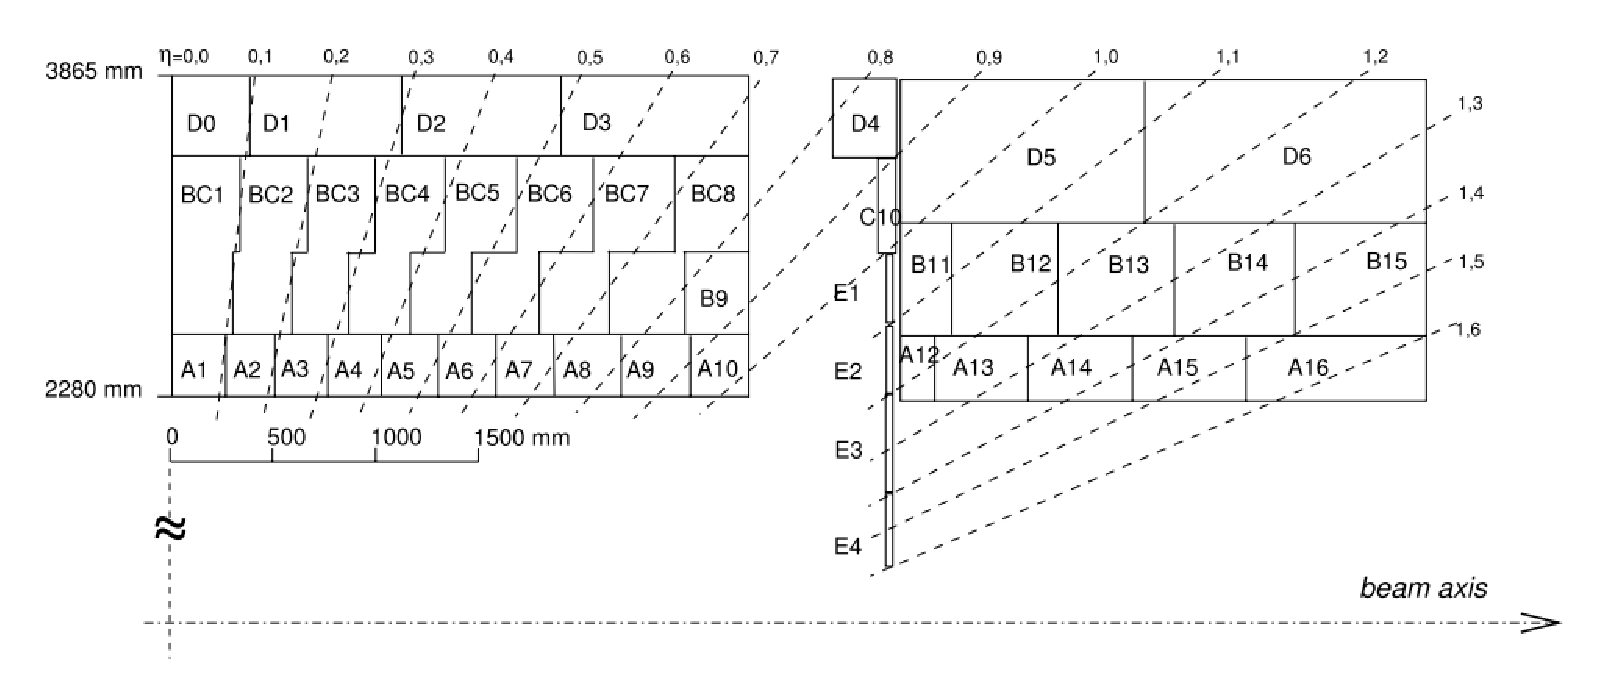
\includegraphics[width=0.\textwidth]{detector/figures/extendedbarrel}}
	\caption{Schematic of a section of TileCal barrel and extended barrel modules, with the
        cells division. The parts labelled with ``E'' are the MBTS.\label{fig:extendedbarrel}}
\end{center}\end{figure}


\section{Trigger system}\label{sec:trigger}

It was already introduced at the beginning of this Chapter the issue
faced by LHC experiments of dealing with a huge amounts of events
at very high frequencies. We remind that considering the nominal LHC
luminosity of \highL\ a rate of interactions of 40~MHz is expected!
This poses serious technical difficulties as the maximum frequency
at which data can be recorded is limited to 200~Hz considering the
limited capacity for storage.

ATLAS developed a trigger system able to reduce by a factor of 10$^6$
the amount of data to be kept by selecting only interesting physics events.
The system is divided in three levels characterized by increasing sofistication
and diminishing speed. At the very first indeed we will need a really quick and
simple criterium to reject uninteresting events. The reduced information can then be
processed with somehow slower logic by the other two High Level Triggers (HLT).
A drawing of the system is shown in Figure~\ref{fig:trigger}.

\begin{figure}[tb]\begin{center}
	\subfigure{
  	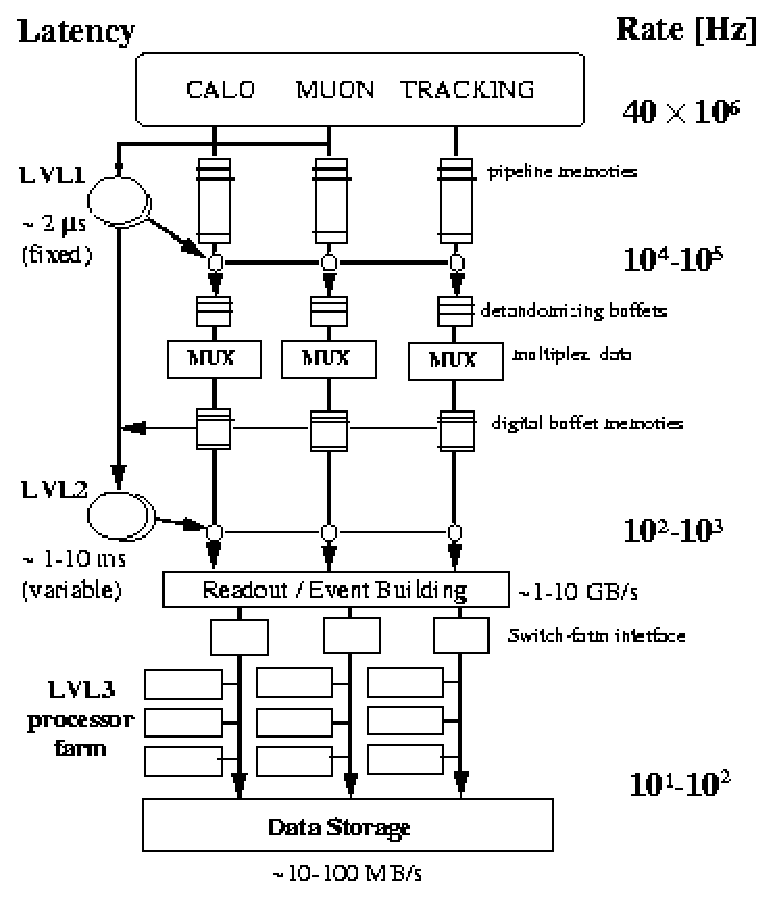
\includegraphics[width=0.5\textwidth]{detector/figures/triggerscheme}}
	\caption{Schematic drawing of the three-level trigger system of ATLAS.\label{fig:trigger}}
\end{center}\end{figure}

Most of the trigger chains used for physics are un-scaled in the
sense that all the events passing the selection are kept, but there
are also pre-scaled trigger chains that contain either too many events
or events considered not physically interesting. These trigger chains
are used for checks or calibration rather than physics analysis, and the
prescaling value $P$ means that of all the events that would have passed 
the trigger, $1/P$ were accepted.

With the term ``trigger chain'' we refer to the sequence of selections
defining a certain trigger object, with a naming convention like:
\begin{equation*}\label{eq:}
{\rm [LEVEL][N][TYPE(S)][THRESHOLD][ISOLATION][QUALITY]},
\end{equation*}
where the components, from left to right, are: the trigger level used; the
multiplicity of the type; the object candidate; the threshold applied to
the transverse momentum or energy of the object candidate; the object isolation;
the severity of the final algorithm requirements (this applies only to the Event
Filter level).

Trigger chains define a {\it trigger menu}, where they are associated to their
prescale value $P$, and which is chosen based on the physics program of the
data taking period taking into account the LHC luminosity. 

Defining the data taking period time unit as ``Luminosity Block'' (LB), typically
a few minutes of  data taking, information on beam conditions, detector performance 
and events passing any of the trigger chains of the trigger menu are stored
to be then used in the analyses. All the LB occurring between the start and the
end of a stable beam collision period compose a ``run''. Runs are finally grouped
in ``Data Periods'', labelled with capital letters (``Period A'', ``Period B'', {\it etc}.),
when they pertain to the same general detector condition, machine configuration and
trigger menu.




\subsection{Level 1 trigger}\label{sec:lvl1}

The Level 1 trigger (L1) is completely based on the hardware of the detector,
taking information from calorimeters, from the muon spectrometer trigger
systems RPC and TGC (Section~\ref{sec:muonspec}) and from the MBTS (Section~\ref{sec:forward}) 
at 40~MHz (the frequency of the beam crossing) and reducing it to 75~kHz by choosing events with high
transverse momentum or high missing transverse energy.

Using dedicated fast front-end electronics (the typical decision time being less than
2~$\mu$s), calorimeter cells are analogically 
summed to build calorimetric towers which, if having an energy higher than a 
certain threshold, will activate a trigger chain.

These trigger chains will then be combined with the information from the
muon spectrometer to form the so-called Region of Interest (RoI) that is
passed to the next trigger level.


\subsection{Level 2 trigger}\label{sec:lvl2}

Starting from the RoI, the Level 2 trigger (L2) will reduce the 75~kHz to
3.5~kHz of events with an average decision time of 40~ms. At this
stage the information from the trackers is incorporated to the RoI
to build candidate object (electrons, photons, muons) and 
better obtain its position and energy with simplified algorithms
quick enough to respect the limit on the decision time.

\subsection{Event filter}\label{sec:lvl3}

The last trigger, Level 3, is called Event Filter (EF) since
at this point the physics objects are built using the same
algorithms as the off-line reconstruction, with looser selections. With an execution time
amounting to 4~s, the EF reduces the event rate to the goal value
of 200~Hz.
Events passing the EF are assigned to {\it streams} defined to separate
the events into different datasets for different analysis interests, e.g.
electron streams, muon streams, jet streams {\it etc}.

As an example, one of the trigger chains used in our analysis is 
\texttt{EF\_mu24i\_tight}: it selects events at the EF level with one 
muon with $p_T>24$~\gev\ and some isolation requirement which passes
the muon reconstruction algorithm cuts defined as ``tight''
(more on event reconstruction is reported in the dedicated Chapter~\ref{chap:objects}).

\section{Data Quality}\label{sec:daq}

The totality of p-p collisions recorded by ATLAS, which differs from the amount
delivered by the LHC because of data-taking inefficiencies, is still
not 100\% usable by physics analyses. Indeed, every subdetector needs to
perform some routine checks %(usually done by PhD students) 
on the quality of the data they recorded in order to certify that its performace
was conform to the expectations. So-called ``Good Runs Lists'' (GRL) are
compiled stating for each LB what was ``OK'' and what not.
The single analyses will then decide which GRL to use, based on their specific
needs of the individual subsystems.


\clearpage{\pagestyle{empty}\cleardoublepage}
\clearpage{\pagestyle{empty}\cleardoublepage}

\chapter{Monte Carlo simulation and SM background samples}\label{chap:mc}


\clearpage{\pagestyle{empty}\cleardoublepage}
\clearpage{\pagestyle{empty}\cleardoublepage}

\chapter{Objects reconstruction}\label{chap:objects}

\section{Electrons}\label{sec:electrons}
\section{Muons}\label{sec:muons}
\section{Jets}\label{sec:jets}



\clearpage{\pagestyle{empty}\cleardoublepage}
\phantomsection
\addcontentsline{toc}{chapter}{Part II}
\input{smallstuff/pII.tex}
%\chapter*{Part II}
\clearpage{\pagestyle{empty}\cleardoublepage}
\clearpage{\pagestyle{empty}\cleardoublepage}

\chapter{Searches for vector-like top partner pairs in the single lepton channel}~\label{chap:vlq}

Starting from this chapter, and continuing in Chapter~\ref{chap:wbx} 
and Chapter~\ref{chap:htx}, we are going to describe two 
searches for vector-like top partners \TTbar\ pairs performed in the single 
lepton\footnote{In the following, with the word ``lepton'' we will 
refer either to an electron or a muon, assumed to come from the leptonic
decay of a $W$ boson or a leptonic $\tau$ decay.}
%with its associated neutrino, which is considered to be the only particle contributing to the transverse missing energy \met.}
 channel. These analyses
are optimized for different final states and are thus complementary.
The analyses are performed using a partial dataset of the pp collisions at the \cme\ 
of \rts=8~\tev\ collected during 2012 at the ATLAS detector, corresponding to an integrated luminosity of  14.3~\ifb.
The first search focuses on  vector-like top partners decay channels with high 
Branching Ratio (BR) to 
a $W$ boson and a bottom quark, while the second search is optimized for events with 
high BR to a Higgs boson and a top quark.
%and is performed using the full dataset of pp collisions at the \cme\ of \rts=8~\tev\ collected during 2012 at the ATLAS detector, consinsting in 20.34~\ifb, while
%search for vector-like top partners with high BR to $Ht$
%uses a partial dataset of the same data, amounting to 14.3~\ifb.

This chapter is devoted to the presentation of the general features that are common to 
the two analyses and is organized as follows: first in Section~\ref{sec:strategy}
we review the strategy for vector-like quark searches adopted 
by the Exotics group of the ATLAS collaboration; Section~\ref{sec:presel}
summarises the common event preselection for data and few general concepts in the
analyses design; Section~\ref{sec:datasets}
describes the Monte Carlo samples used in the searches, which
are in general common to both analyses with only few exceptions that are reported,
and how the multi-jet background from QCD events is
obtained; Section~\ref{sec:systematics} introduces the general treatment of systematic uncertainties.
%The two analyses are then presented in details in Chapter~\ref{chap:wbx} 
%(\TTbar\ pairs decaying to \wbx\ ) and in Chapter~\ref{chap:htx}
%(\TTbar\ pairs decaying to \htx\ ). The final results are presented 
%in Chapter~\ref{chap:results}.

\section{General strategy for vector-like quark pairs searches}\label{sec:strategy}

The phenomenology for vector-like quarks was described already in Section~\ref{sec:THvlq}
of this dissertation. Here we will only briefly re-introduce the concepts on which
the strategy for the searches has been built. Table~\ref{tab:vlqdecays} collects the 
decay modes for vector-like quarks in the singlet and doublet models. It is evident
from the richness of the final state phase space, combined with the unpredicted mass
of the heavy objects that could span from few hundreds of \gev s (down to the values exluded by
previous searches) up to  $\sim 1$~\tev\ (since we focus on pair production of vector-like
quarks, which is favoured up to this mass scale)% as shown in Figure~\ref{fig:vlqxsec}), 
that is impossible to cover it with a single inclusive search.

\begin{table}[htb]\centering
\begin{tabular}{|lc|lc|}\toprule
\hskip2ex VLQ &  Decay & \hskip2ex VLQ  & Decay \\ 
\hskip1ex Singlets &  modes & \hskip1ex Doublets & modes\\
& & &\\
$T(+2/3)$ & $W^+b,\, Ht,\, Zt$ & \multirow{2}{*}{$\quad\bigg(\begin{array}{c}T \\ B\end{array}\bigg)$} & $W^+b,\, Ht,\, Zt$\\ 
& & & $ W^-t,\, Hb,\, Zb$\\
$B(-1/3)$ & $ W^-t,\, Hb,\, Zb$ & & \\
& & \multirow{2}{*}{$\quad\bigg(\begin{array}{c}T \\ X\end{array}\bigg)$} & $Ht,\, Zt$\\
$X(+5/3)$ & $W^+t$ & & $W^+t$\\
& & &\\
$Y(-4/3)$ & $W^-b$ & \multirow{2}{*}{$\quad\bigg(\begin{array}{c}B \\ Y\end{array}\bigg)$} & $Hb,\, Zb$\\
& & & $W^-b$\\\bottomrule
\end{tabular}
\caption{Allowed decay modes for vector-like singlets and doublets.}\label{tab:vlqdecays}
\end{table}

%\begin{figure}[htb]\begin{center}
%	\subfigure{
%  	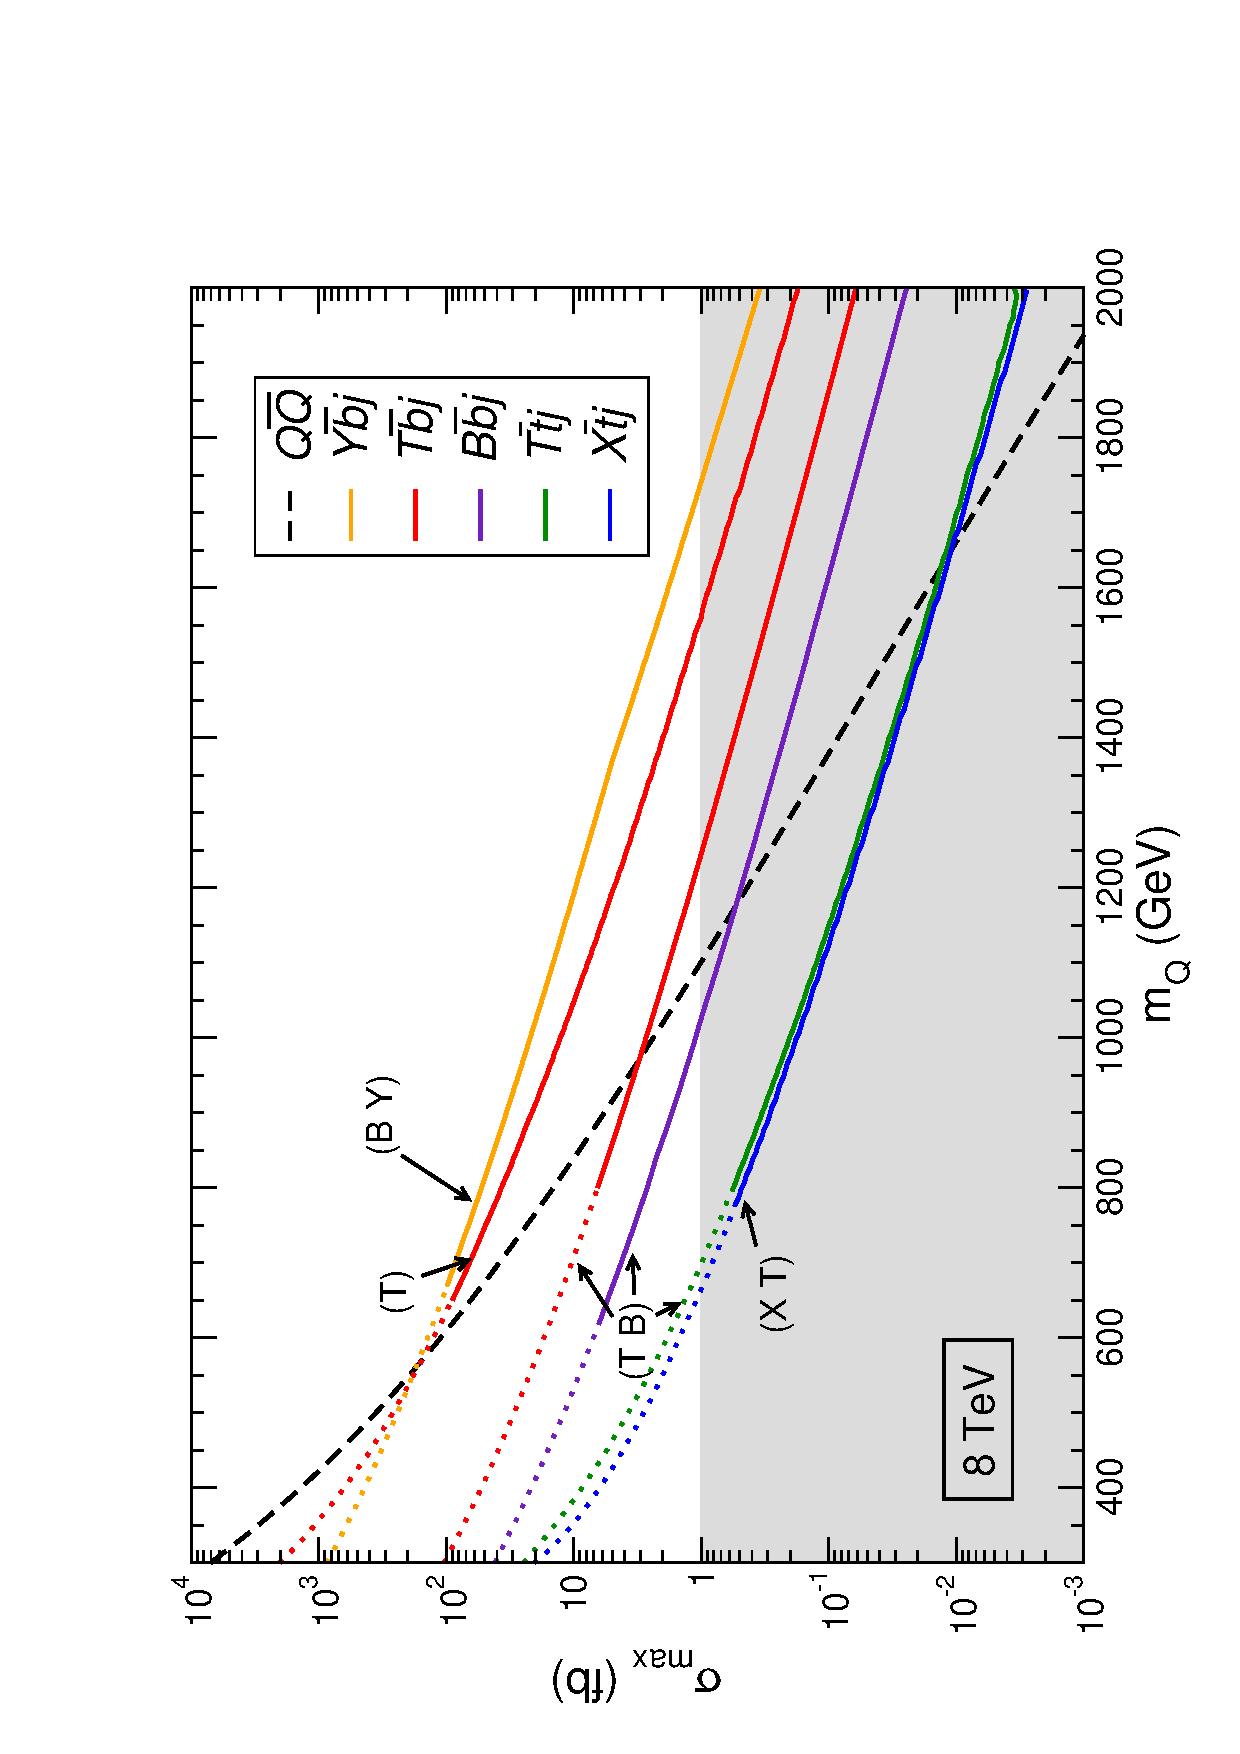
\includegraphics[width=0.65\textwidth, angle=270]{vlq_analysis/figures/xsec-8}}
%	\caption{\label{fig:vlqxsec} Pair and single production cross sections  for heavy 
%        quarks in proton-proton collisions at $\sqrt{s}=8$~TeV~\cite{Aguilar-Saavedra:2013qpa}.}
%\end{center}\end{figure}

The BR of vector-like top and bottom partners to the allowed decay modes depends
on the mass of the heavy quark and on the considered model (in our case, singlet or doublet
scenario), as shown in Figure~\ref{fig:vlqBRs}.
Each decay mode has specific features that allow to define powerful, optimized searches.
Therefore in order to exploit this opportunity and at the same time stay as model independent
as possible, different searches for vector-like quarks are performed at ATLAS
to be later combined, each of them sensitive to specific channels.
To ensure a comprehensive coverage of the phase space, a two-dimensional plane is defined 
(Figure~\ref{fig:2dplane}) as follows:
along the Y axes is the BR of the decay 
modes with a Higgs boson in the final state; along the X axis is the BR 
of the decay modes with a $W$ boson in the final state.
The BR to the channel with a $Z$ boson in the final state is then fixed by the 
unitarity requirement BR($T/B\to  Zt/b$) = 1 - BR($T/B\to Ht/b$) - BR($T/B\to Wb/t$).
A plane of this kind is defined for every vector-like quark mass point considered 
in the analysis. Each point of each plane therefore represents a 
uniquely defined model, and analyses are performed for every configuration
to either find deviations from expectations or to set a 95\% Confidence Level (CL) exclusion.
The final objective of the joint strategy is to cover the full plane by combining
analyses probing the different signatures.

\begin{figure}[h!tb]\begin{center}
	\subfigure[]{\label{fig:vltBRs}
  	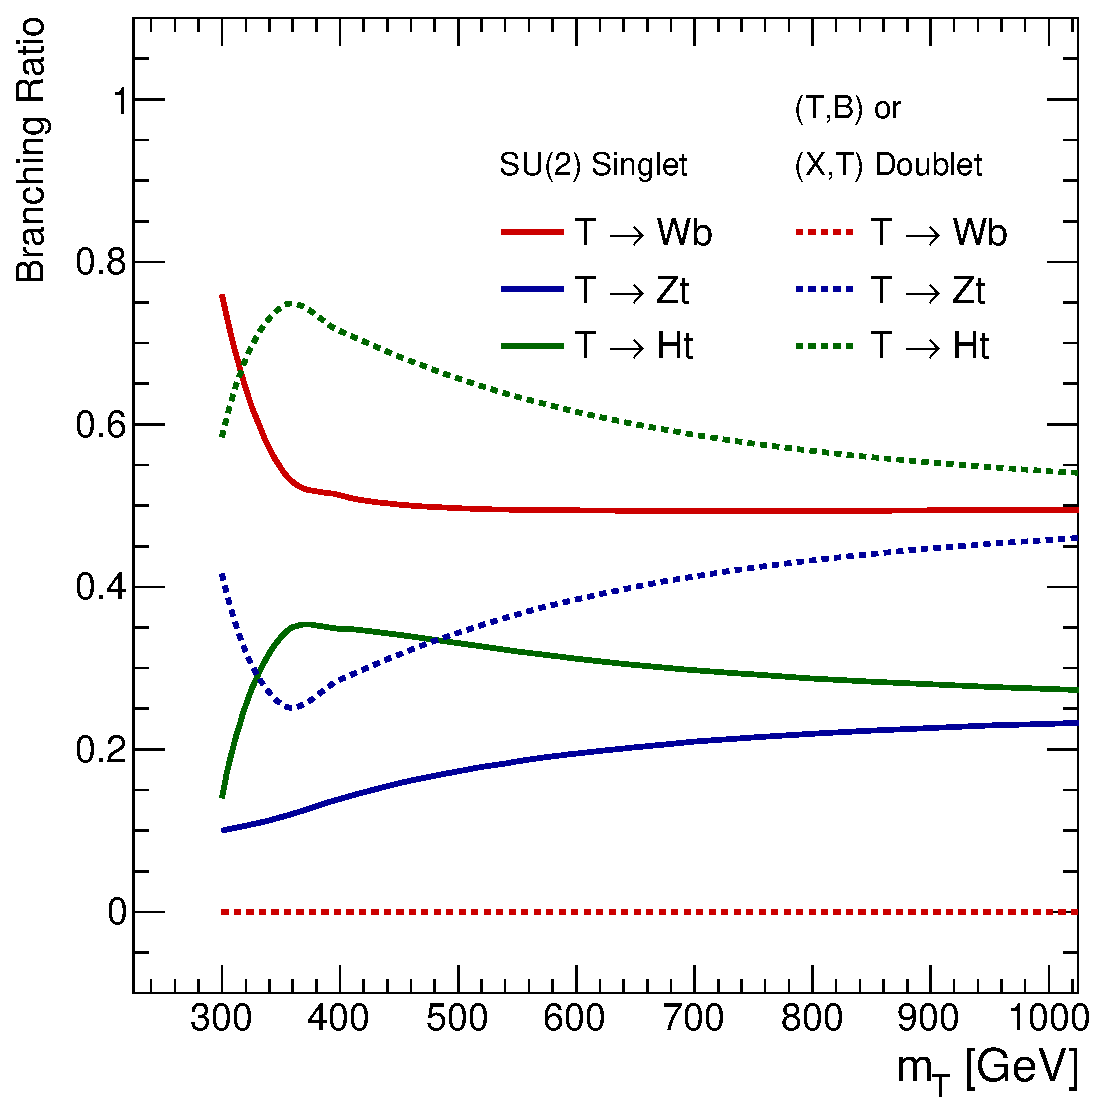
\includegraphics[width=0.47\textwidth]{vlq_analysis/figures/fig_02a.eps}}
	\subfigure[]{\label{fig:vlbBRs}
  	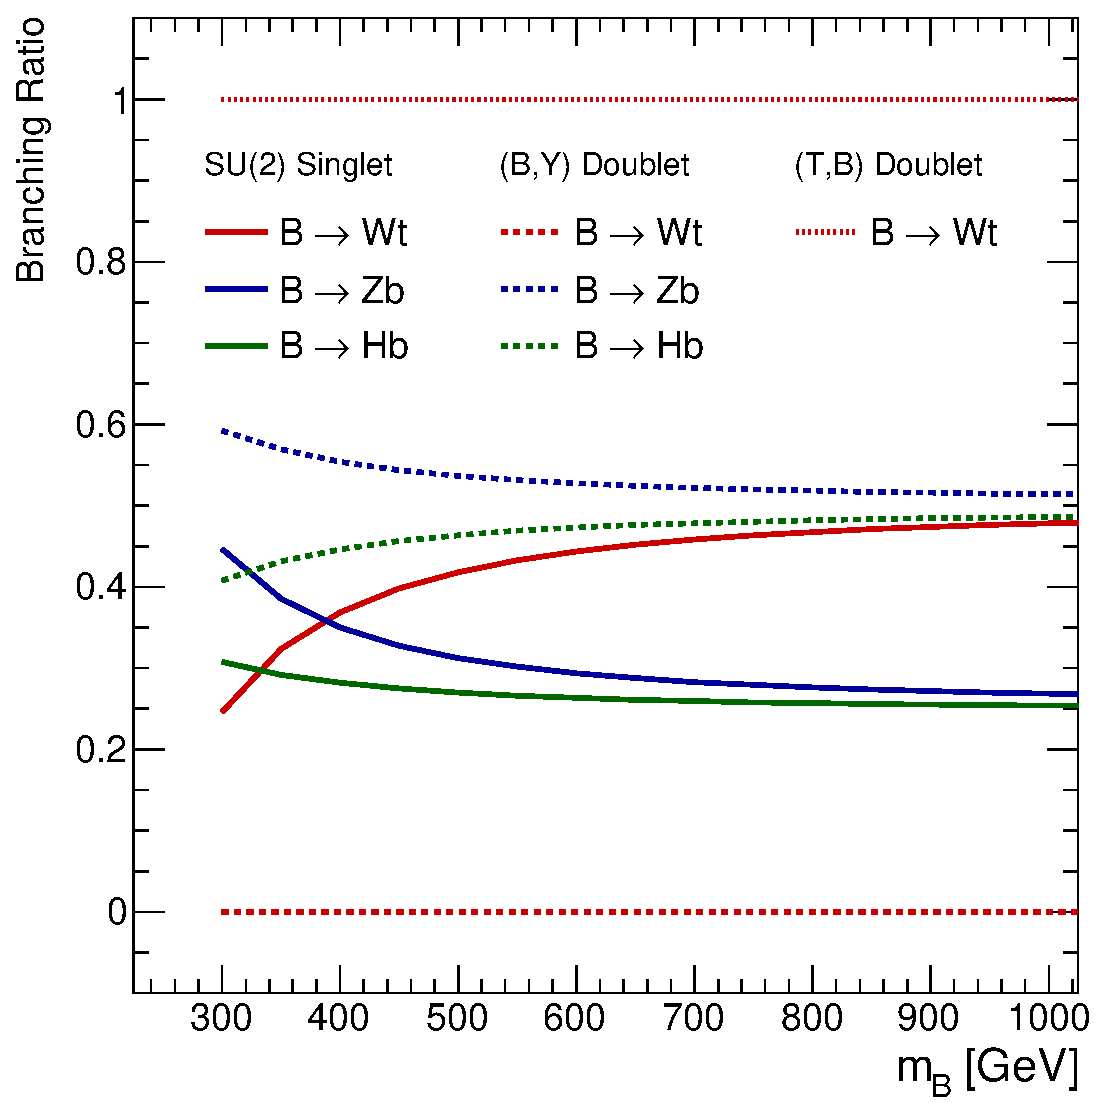
\includegraphics[width=0.47\textwidth]{vlq_analysis/figures/fig_02b.eps}}
	\caption{Branching ratio of vector-like top (a) and bottom (b) partners as a function of the heavy quark mass $m_T$ and $m_B$ respectively~\cite{ATLAS-CONF-2013-056} for singlet and doublet models.\label{fig:vlqBRs}}
\end{center}\end{figure}

\begin{figure}[h!bt]\begin{center}
	\subfigure{
        \begin{pgfpicture}{0.0\textwidth}{0.0\textheight}{.5\textwidth}{.5\textwidth}
%\begin{pgfpicture}{0.0\textwidth}{0.0\textheight}{1.\textwidth}{.6\textwidth}

\begin{pgfscope}
\pgfsetendarrow{\pgfarrowlargepointed{6pt}}
\pgfsetlinewidth{1.5pt}

\begin{pgftranslate}{\pgfpoint{0.05\textwidth}{0.05\textheight}}
%\begin{pgftranslate}{\pgfpoint{0.1\textwidth}{0.15\textheight}}
  {
    %\color{black}
    \color{black!50!red}
    \pgfputat{\pgfxy(3.5,-0.5)}{\pgfbox[left,base]{BR($T\to Wb$)}}
  }
  {
    \color{black!50!blue}
    \pgfputat{\pgfxy(3.5,-0.8)}{\pgfbox[left,base]{BR($B\to Wt$)}}
  }
  {
    \begin{pgfrotateby}{\pgfdegree{90}}
      {
        \color{black!50!red}
        \pgfputat{\pgfxy(3.5,0.4)}{\pgfbox[left,base]{BR($T\to Ht$)}}
      }
      {
        \color{black!50!blue}
        \pgfputat{\pgfxy(3.5,0.7)}{\pgfbox[left,base]{BR($B\to Hb$)}}
      }
    \end{pgfrotateby}
  }
  {
    \pgfsetlinewidth{1.5pt}
    \color{gray!30!white}%\color{light-gray}
    \pgfmoveto{\pgfxy(5,0)}
    \pgflineto{\pgfxy(5,5)}
    \pgflineto{\pgfxy(0,5)}
    %\pgfstroke
    \pgffill
  }
  {
    %\color{black}
    \pgfputlabelrotated{0.5}{\pgfxy(0,5)}{\pgfxy(5,0)}{8pt}{\pgfbox[center,base]{Forbidden}}
  }
  \begin{pgfscope}
    \pgfmoveto{\pgfxy(5,0)}
    \pgflineto{\pgfxy(0,0)}
    \pgflineto{\pgfxy(0,5)}
    {
      \color{yellow!30!white}
      \pgfclip
      \pgfcircle[fill]{\pgfxy(.5,4)}{35pt}
    }
    {
      \pgfputat{\pgfxy(0.15,3.6)}{\pgfbox[left,base]{\large{\color{black!70!red}$Ht$}{\color{black!70!blue}$(b)$}}}
    }
    {
      \color{yellow!30!white}
      \pgfcircle[fill]{\pgfxy(.6,.6)}{35pt}
    }
    {
      \pgfputat{\pgfxy(0.15,.4)}{\pgfbox[left,base]{\large{\color{black!70!red}$Zt$}{\color{black!70!blue}$(b)$}}}
    }
    {
      \color{yellow!30!white}%\color{light-gray}
      \pgfcircle[fill]{\pgfxy(4,0)}{35pt}
    }
    {
      \pgfputat{\pgfxy(3.2,0.4)}{\pgfbox[left,base]{\large{\color{black!70!red}$Wb$}{\color{black!70!blue}$(t)$}}}
    }
  \end{pgfscope}
  {
    %\color{black}
    \pgfsetendarrow{\pgfarrowlargepointed{6pt}}
    \pgfsetlinewidth{1.5pt}
    \pgfline{\pgfxy(0,0)}{\pgfxy(5.5,0)}
    \pgfstroke
    %\pgfsetendarrow{\pgfarrowlargepointed{6pt}}
    %\pgfsetlinewidth{1.5pt}
    \pgfline{\pgfxy(0,0)}{\pgfxy(0,5.5)}
    \pgfstroke
  }

\end{pgftranslate}
\end{pgfscope}
\end{pgfpicture}
}
       	\caption{Two dimensional plane used to represend the comprehensive scan of model mixing. Searches 
        with a Higgs boson in the final state cover the top left corner; searches with a $Z$ boson in the 
        final state cover the bottom left corner; searches with a $W$ boson in the final state cover the 
        bottom right corner. The shaded area labelled as ``forbidden'' is the unphysical region where
        BR($T/B\to Ht/b$) + BR($T/B\to Wb/t$) + BR($T/B\to  Zt/b$) $>1$ \label{fig:2dplane}}
\end{center}\end{figure}


Up to the date of the writing of this dissertation, four complementary 
and quasi model-independent analyses have been performed by the Exotics working
group on the partial dataset of 14.3~\ifb\ of proton-proton collision data at 
$\sqrt{s}=8\tev$.  
Two analyses investigated dilepton channels and two probed single lepton channels.

The search for vector-like bottom and top partners in the same-sign 
dilepton channel~\cite{ATLAS-CONF-2013-051}
investigates a channel
with very small contamination from Standard Model backgrounds and
is also sensitive to four-top production $pp\to t\bar{t}t\bar{t}$, 
either through the Standard Model process or a beyond-SM source such as 
pair production of scalar color-octets (sgluons) or gluinos, with subsequent 
decays to top quark pairs.
The approach of this search is to select via restrictive cuts (that also
impose a veto on a $Z\to l\bar{l}$ boson) the eventual signal
and compare the final counts with the expected yields from background sources.
Figure~\ref{fig:feyndSS} shows how the decays of vector-like bottom and top partner
pairs can contribute to the same-sign dilepton signature. From this it is easy to
understand that this search will be mainly covering the bottom right corner
of the \BBbar\ two dimensional plane of Figure~\ref{fig:2dplane} and the top 
left corner of the same plane for \TTbar.
%Data-driven techniques are used to evaluate the background contribution to the signal region coming from charge misidentification and fakes, the two main sources of background. In the end 3, 10 and 2 events are observed in the $ee$, $e\mu$ and $\mu\mu$ channels respectively. The observed counts are consistent with the expected yields in the $ee$ and $\mu\mu$ channel. A small excess of events is observed in the $e\mu$ channel, leading to a slightly weaker limit than expected, but still within a $\pm1\sigma$ band.
%These counts are consistent with the expected yields, except for the  $e\mu$ channel.

\begin{figure}[hbt]
\begin{center}
        \myskip\begin{fmffile}{fmfssBBTT}
\unitlength=1mm
\hskip-5ex
\subfigure[]{\label{fig:feyndSSBB}
    \begin{fmfgraph*}(60,30)
      \fmfleft{i1,i2}
      \fmfright{o1,o2,o3,o4,o5,o6,o7,o8}
      \fmflabel{$g$}{i1}
      \fmflabel{$g$}{i2}
      %\fmflabel{$b$}{}
      %%%%
      \fmf{phantom}{o1,v4,v3,v2,v1,i1}
      \fmf{phantom}{o2,v4,v3,v2,v1,i1}
      \fmf{phantom}{o3,v5,v3,v2,v1,i1}
      \fmf{phantom}{o4,v5,v3,v2,v1,i1}
      %%%%
      \fmf{phantom}{o5,v7,v6,v2,v1,i2}
      \fmf{phantom}{o6,v7,v6,v2,v1,i2}
      \fmf{phantom}{o7,v8,v6,v2,v1,i2}
      \fmf{phantom}{o8,v8,v6,v2,v1,i2}
      %%%%
      \fmflabel{$\bar{b}$}{o1}
      \fmflabel{\textcolor{red}{$W^{-}$}}{o2}
      \fmflabel{\textcolor{blue}{$W^{+}$}}{o4}
      \fmflabel{\textcolor{red}{$W^{-}$}}{o8}
      \fmflabel{\textcolor{blue}{$W^{+}$}}{o6}
      \fmflabel{$b$}{o5} 
      \fmf{plain}{o1,v4}
      \fmf{photon}{o2,v4}
      %%
      \fmf{photon}{o4,v3}
      \fmf{plain}{o5,v7}
      \fmf{photon}{o6,v7}
      \fmf{photon}{o8,v6}
      %%%
      \fmf{plain,label=$\bar{B}$}{v2,v3}
      \fmf{plain,label=$B$}{v2,v6}
      \fmf{plain,label=$\bar{t}$,l.dist=-7thick}{v4,v3}
      \fmf{plain,label=$t$}{v7,v6}
      \fmf{curly}{i1,v1}
      \fmf{curly}{i2,v1}
      \fmf{curly,label=$g$,l.dist=-7thick}{v1,v2}
    \end{fmfgraph*}
}\hskip5ex
\subfigure[]{\label{fig:feyndSSTT}
    \begin{fmfgraph*}(60,30)
      \fmfleft{i1,i2}
      \fmfright{o1,o2,o3,o4,o5,o6,o7,o8}
      \fmflabel{$g$}{i1}
      \fmflabel{$g$}{i2}
      %\fmflabel{$b$}{}
      %%%%
      \fmf{phantom}{o1,v4,v3,v2,v1,i1}
      \fmf{phantom}{o2,v4,v3,v2,v1,i1}
      \fmf{phantom}{o3,v5,v3,v2,v1,i1}
      \fmf{phantom}{o4,v5,v3,v2,v1,i1}
      %%%%
      \fmf{phantom}{o5,v7,v6,v2,v1,i2}
      \fmf{phantom}{o6,v7,v6,v2,v1,i2}
      \fmf{phantom}{o7,v8,v6,v2,v1,i2}
      \fmf{phantom}{o8,v8,v6,v2,v1,i2}
      %%%%
      \fmflabel{\textcolor{red}{$\bar{t}, \bar{t}$}$, \bar{b}$}{o1}
      \fmflabel{$Z, H,$ \textcolor{red}{$W^-$}}{o3}
      \fmflabel{$\bar{b}$}{o7}
      %\fmflabel{\textcolor{red}{$W^{-}$}}{o2}
      \fmflabel{\textcolor{blue}{$W^{+}$}}{o8}
      \fmflabel{\textcolor{red}{$W^{-}$}}{o5}
      \fmflabel{\textcolor{blue}{$W^{+}$}}{o6}
      %\fmflabel{}{o5} 
      \fmf{plain}{o1,v4}
      \fmf{photon}{o3,v4}
      %%
      %\fmf{photon}{o4,v3}
      \fmf{photon}{o5,v7}
      \fmf{photon}{o6,v7}
      \fmf{plain}{o7,v8}
      \fmf{photon}{o8,v8}
      %%%
      \fmf{plain,label=$\bar{T}$,l.dist=-6thick}{v2,v4}
      \fmf{plain,label=$T$}{v2,v6}
      %\fmf{plain,label=$\bar{t}$,l.dist=-7thick}{v4,v3}
      \fmf{plain,label=$t$}{v6,v8}
      \fmf{dashes,label=$H$,l.dist=-6thick}{v7,v6}
      \fmf{curly}{i1,v1}
      \fmf{curly}{i2,v1}
      \fmf{curly,label=$g$,l.dist=-7thick}{v1,v2}
    \end{fmfgraph*}
}
\end{fmffile}
\myskip
	\caption{Feynman diagrams for \BBbar\ (left) and \TTbar\ (right)
        decays that can result in a final state with two same-sign leptons,
        in the case that the same-sign $W$ bosons (highlighted in different colors;
        on the right the anti-top quarks associated to the $Z$ or Higgs bosons are
        also highlighted as they will originate a $W^{-}$ boson) decay
        into a lepton and a neutrino. \label{fig:feyndSS}}
\end{center}
\end{figure}


The search in the opposite-charge dilepton channel~\cite{ATLAS-CONF-2013-056} 
focuses on vector-like bottom  (top) partners decay channels where at least one 
heavy quark decays into a $Z$ boson and a bottom (top) quark. 
Here the strategy is to reconstruct the $Z$ boson from the opposite-charge lepton
pair and use the invariant mass of the $Z$ boson candidate paired  with the highest 
$p_T$ $b$-jet as final discriminant variable to perform the statistical analysis.
It is then straight-forward to expect this search to efficiently cover the bottom
left corners of both the \BBbar\  and \TTbar\  two dimensional planes of
Figure~\ref{fig:2dplane}.


The searches in the single lepton channel are focused on vector-like top partner
pairs decays and are optimized for two distinctive signatures. One search
exploits the boosted kinematics of the $W$ boson from vector-like top partners decays
to reconstruct it from its hadronic channel final state 
particles~\cite{ATLAS-CONF-2013-060}. The heavy quark invariant mass is 
then reconstructed pairing the boosted  $W$ boson  with a \bjet\ and this
distribution is used to perform the statistical analysis. It is evident that this
search is going to cover the bottom right corner of the \TTbar\  two dimensional plane 
of Figure~\ref{fig:2dplane}.

The other search in the single lepton channel considers final states with high
jet and \bjet\ multiplicities as a result of the decay of at least one heavy quark
into a Higgs boson (assumed to decay into \bbbar) and a top 
quark~\cite{ATLAS-CONF-2013-018} (see Figure~\ref{fig:feyndHTX}). The distribution
of the  total transverse momentum of the event is then used to perform the statistical 
analysis. This search is mainly sensitive to the top left corner of the \TTbar\  
two dimensional plane of Figure~\ref{fig:2dplane}.


\begin{figure}[hbt]
\begin{center}
        \myskip\begin{fmffile}{fmfTThtx}
\unitlength=1mm
\begin{fmfgraph*}(60,50)
  \fmfleft{i1,i2,i3,i4,i5,i6,i7,i8}
  \fmfright{o1,o2,o3,o4,o5,o6,o7,o8}
  \fmflabel{$g$}{i3}
  \fmflabel{$g$}{i6}
  %\fmflabel{$b$}{}
%%%%
  \fmf{phantom}{i1,v11,v12,v13,v14,o1}
  \fmf{phantom}{i2,v21,v22,v23,v24,o2}
  \fmf{phantom}{i3,v31,v32,v33,v34,o3}
  \fmf{phantom}{i4,v41,v42,v43,v44,o4}
  \fmf{phantom}{i5,v51,v52,v53,v54,o5}
  \fmf{phantom}{i6,v61,v62,v63,v64,o6}
  \fmf{phantom}{i7,v71,v72,v73,v74,o7}
  \fmf{phantom}{i8,v81,v82,v83,v84,o8}
  \fmffreeze
  \fmflabel{$\bar{t}, \bar{t}, \bar{b}$}{o1}
  \fmflabel{$Z, H, W^-$}{o3}
  \fmf{plain}{o1,v32}
  \fmf{photon}{o3,v32}
  \fmf{plain,label=$t$}{v62,v73}
  \fmflabel{$b$}{o6}
  \fmf{photon,label=$W^+$}{v74,v73}
  \fmf{plain}{o8,v74,o7}
  \fmflabel{$l^+$}{o8}
  \fmflabel{$\bar{\nu}_l$}{o7}
  \fmf{plain}{o6,v73}

  \fmf{dashes,label=$H$}{v62,v53}
  \fmf{plain}{o5,v53,o4}
  \fmflabel{$b$}{o5}
  \fmflabel{$\bar{b}$}{o4}
  %\fmf{photon,label=$H$}{v10,v11}
  %\fmf{plain}{v9,v10,v12}
  %\fmflabel{$b$}{v9}
  %\fmflabel{$\bar{b}$}{v12}
  \fmf{plain,label=$T$}{v62,v61}
  \fmf{plain,label=$\bar{T}$}{v32,v31}
  \fmf{curly}{i3,v31}
  \fmf{curly}{i6,v61}
  \fmf{plain}{v31,v61}
\end{fmfgraph*}
\end{fmffile}
\myskip
	\caption{Feynman diagrams for the $\TTbar\to Ht+X$
        decay entering the high jet and \bjet\ multiplicity final states.
        Assuming the single lepton condition, in this picture all the bosons 
        produced in the $\Tbar$ decay will decay hadronically.\label{fig:feyndHTX}}
\end{center}
\end{figure}



We will in the following treat in details the two searches for vector-like 
top partners performed in the single lepton channels, starting with the
discussion of the common features between the two analyses.


\section{Data sample and common event preselection}\label{sec:presel}

The data from pp collision events recorded at the ATLAS experiment during
2012 at a \cme\ of $\rts=8\tev$ are considered. Physics object definitions 
were discussed in Chapter~\ref{chap:objects}.
Events collected during
stable beam periods are required to pass data quality requirements and
single lepton trigger selection. In order to maximize trigger
efficiency, different transverse momentum threshold triggers are combined
through a logical \OR, with the lower \pt\ ones including isolation requirements
that result in inefficiencies for high \pt\ lepton candidates, recovered with
the use of the higher threshold triggers. The electron triggers have
\pt\ thresholds of 24 and 60~\gev, the muon ones of 24 and 36~\gev\ (Section~\ref{sec:REQtrigger}).

After passing trigger requirements, events with more than one lepton are
discarded. In addition, the only lepton of the event has to match within $\dr<0.15$ the
triggered one. As basic preselection, four jets satisfying the conditions
described in Section~\ref{sec:jets} are required, at least one of them
being tagged as a \bjet.

In order to suppress the multi-jet background from QCD processes,
combined cuts on the \met\ and on the tranverse mass of the 
leptonically decaying $W$ boson \mt\footnote{$\mt = \sqrt{2 p^\ell_{\rm T} \met (1-\cos\Delta\phi)}$, with
$p^\ell_{\rm T}$  being the transverse momentum (energy) of the muon (electron) and $\Delta\phi$ the
azimuthal angle separation between the lepton and the direction of
the missing transverse momentum.}\ 
are defined: $\met>20~\gev$ and $\met+\mt>60~\gev$.

At this point, a simple consideration about the typical expected jet
(and \bjet) multiplicity based on counting the parton multiplicities and their 
flavor is made so as to define an orthogonality
cut between the two analyses. Table~\ref{tab:jetmult} shows the 
number of jets (\bjet s) per decay channel combinations of \TTbar\ pairs, 
in the case of single lepton selection with at least four jets
(i.e. one $W$ boson will always decay into lepton and neutrino,
and $Z$ boson decay to neutrinos is excluded in the $WbZt$ channel) and assuming that
the Higgs boson decays to a bottom quark-antiquark pair.
To avoid overlap between selected events from the two analyses, in the
\wbx\ analysis events with $\geq$6 jets and $\geq$3 \bjet s are 
rejected\footnote{As will be explained later in Section~\ref{sec:htxEVT}, another orthogonality
cut will be applied in the low \bjet\ multiplicity channel of the \htx\ analysis.}.

\begin{table}\centering
\begin{tabular}{lccc}\toprule
& $Wb$ & $Ht$ & $Zt$ \\\midrule
&\cellcolor{lightgray} & & \cellcolor{lightgray}\\
\multirow{-2}{*}{$Wb$} & 
\cellcolor{lightgray}\multirow{-2}{*}{\bf 4 (2)} & 
\multirow{-2}{*}{6 (4)} & 
\cellcolor{lightgray}\multirow{-2}{*}{{\bf 6} ({\bf2}/4)} \\
\multirow{2}{*}{$Ht$} & 
\multirow{2}{*}{6 (4)} & 
\multirow{2}{*}{8 (6)} & max: 8 (4/6)\\
& & & \cellcolor{lightgray}min: {\bf6 (2)}\\
\multirow{2}{*}{$Zt$} & 
\cellcolor{lightgray}& max: 8 (4/6) & 
\cellcolor{lightgray}max: {\bf8} ({\bf2}/6) \\
& \cellcolor{lightgray}\multirow{-2}{*}{\bf6 (2/4)} & 
\cellcolor{lightgray}min: {\bf6 (2)} & 
\cellcolor{lightgray}min: {\bf6} ({\bf2}/4)\\
\bottomrule\end{tabular}\caption{Jets (\bjet s) multiplicities in 
the various possible final states. $Z$ boson decays 55\% hadronically, 
15\% of the times into \bbbar, therefore the min/max number of \bjet s 
is reported. Highlighted in bold characters are the channels that after the orthogonality 
cut will contribute to the \wbx\ analysis.}\label{tab:jetmult}
\end{table}




\section{Background and signal modeling}\label{sec:datasets}

All samples are enterely modeled using Monte Carlo simulation with the exception
of QCD multi-jet events, which are derived using data-driven techniques, and 
background from $W$ boson production in association with jets, which is obtained
from Monte Carlo at first but then is normalized to data.

The main background for both analyses is $t\bar{t}$ 
production in association with jets ($t\bar{t}$+jets)
and different choices for the generator are made
in the analyses because of the specific needs of having well
modeled regions.
In the case of the $t\bar{t}$+jets background prediction for the \htx\ analysis 
further corrections to match the data are applied, due to a mismodeling in the
heavy- and light-flavour content of the simulated sample 
(see Section~\ref{sec:htxEVT}).

$W$ boson production  in association with jets ($W$+jets) 
and QCD multi-jet events also contributes, the latter
entering into the event selection via the misidentification of a jet or a photon as an
electron or the presence of a non-prompt lepton from, e.g., semileptonic $b$- or $c$-hadron decay.
Small background contributions originate from single top quark, $Z$+jets, diboson
($WW,WZ,ZZ$), and associated $t\bar{t}V$ ($V=W,Z$) and $t\bar{t}H$ production.

\subsection{Monte Carlo simulated samples}\label{sec:MCbkg}

%All event generators using {\tt HERWIG}~\cite{HERWIG} are also interfaced to {\tt JIMMY v4.31}~\cite{jimmy} to simulate the underlying event.  
With the exception of the 
signal samples, all simulated 
samples utilise {\tt PHOTOS 2.15}~\cite{PhotosPaper} to model
photon radiation and {\tt TAUOLA 1.20}~\cite{TauolaPaper} to model
$\tau$ decays.  

All simulated samples include multiple pp
interactions and make use of the  {\tt GEANT4}~\cite{geant}
detector geometry and response simulation~\cite{atlas_sim}
with the exception of the signal samples, for which a fast simulation of
the calorimeter response is used.

All simulated samples are then processed through the same reconstruction 
software as the data and are reweighted to match 
the instantaneous luminosity profile in data. For more details
on the Monte Carlo simulation chain we refer the reader to
Chapter~\ref{chap:mc} and in particular to Section~\ref{sec:generators}.

%Additional corrections are applied so that the 
%object identification efficiencies, energy
%scales and energy resolutions match those determined in data control
%samples.


\subsubsection{$t\bar{t}$ MC@NLO}\label{subsec:MC@NLO}
Simulated samples of $t\bar{t}$ pair production  in association with jets 
($t\bar{t}$+jets or simply $t\bar{t}$ in the following)
are generated with {\tt MC@NLO} v4.01~\cite{mcatnlo_1,mcatnlo_2,mcatnlo_3} using the {\tt CT10} set of parton distribution functions (PDFs)~\cite{ct10},
with the parton-shower and fragmentation steps being performed by 
{\tt HERWIG} v6.520~\cite{HERWIG}.
The top quark mass is assumed to be equal to $172.5\gev$ and 
the samples are normalized to approximate next-to-next-to-leading-order 
(NNLO) theoretical cross section~\cite{ttbarxs}; the cross section used 
has been computed with {\tt HATHOR 1.2}~\cite{ttbarxs} using the {\tt MSTW2008}
NNLO PDF set~\cite{Martin:2009iq} and is $\sigma_{t\bar{t}}= 238^{+22}_{-24}$~pb, 
where the total uncertainty results from the sum in quadrature of the 
scale and PDF+$\alpha_S$ uncertainties according to 
the {\tt MSTW} prescription~\cite{mstw2}. 
This is the $t\bar{t}$ used in the \wbx\ analysis.

\subsubsection{$t\bar{t}$ Alpgen}\label{subsec:alpgen}
Simulated samples of $t\bar{t}$+jets are generated using
%and $W/Z$+jets events are generated using
the {\tt ALPGEN v2.13}~\cite{ALPGEN} leading-order (LO) generator and the 
{\tt CTEQ6L1} PDF set~\cite{cteq6}, with parton shower and fragmentation  
modelled through {\tt HERWIG} v6.520~\cite{HERWIG}.

A parton-jet matching scheme called ``MLM matching''~\cite{mlm} is used
in orderd to avoid double-counting  of partonic configurations
eventually generated both at the matrix-element calculation level
and at the parton-shower evolution step.

Separate samples are generated for $t\bar{t}$+light jets ($t\bar{t}$+light 
or $t\bar{t}$+LF in the following, from ``light flavour'') 
with up to three additional light partons ($u$, $d$, $s$ quarks or gluons),
and for $t\bar{t}$+heavy-flavour jets ($t\bar{t}$+HF in the following), 
including $t\bar{t}b\bar{b}$ and
$t\bar{t}c\bar{c}$.  
An algorithm based on the angular separation
between the extra heavy quarks is used to remove 
the overlap between $t\bar{t}q\bar{q}$ ($q=b,c$) 
generated from the matrix element calculation and 
from parton-shower evolution in the  $t\bar{t}$+light samples
is employed: matrix-element prediction is chosen over the parton-shower one
when $\Delta R(q,\bar{q})>0.4$, else vice-versa.

%The algorithm used is implemented in the HFOR tool~\cite{hfor}.

Again a top quark mass of $172.5\gev$ is assumed, and normalisation to the
NNLO theoretical cross section is used (see~\ref{subsec:MC@NLO})

\subsubsection{$W/Z$+jets}

Simulated samples of $W/Z$ boson production in association with jets
($W/Z$+jets in the following) are generated with up to five additional 
partons using the {\tt ALPGEN v2.13}~\cite{ALPGEN} LO generator and the 
{\tt CTEQ6L1} PDF set~\cite{cteq6}, interfaced to {\tt HERWIG} v6.520 
for parton showering and fragmentation.
The MLM matching scheme is used also here to avoid double-counting of partonic configurations 
between  matrix-element  calculation and parton showering.

The $W$+jets samples are generated separately for $W$+light jets, 
$Wb\bar{b}$+jets, $Wc\bar{c}$+jets, and $Wc$+jets, 
with the relative contributions normalized using the fraction 
of $b$-tagged jets in $W$+1-jet and $W$+2-jets data 
control samples~\cite{whf}, while
the $Z$+jets samples are generated separately 
for $Z$+light jets, $Zb\bar{b}$+jets, and $Zc\bar{c}$+jets and
normalized to the inclusive NNLO theoretical cross section~\cite{vjetsxs}.
Overlap between $W/Zq\bar{q}$+jets ($q=b,c$) 
events generated from the matrix element calculation and those
generated from parton-shower evolution in the $W/Z$+light jets
samples is avoided via the same algorithm used
for $t\bar{t}$ Alpgen.

\subsubsection{Other backgrounds}\label{subsec:otherbkg}
%,tchanxs,Wtchanxs,schanxs}. 
Simulated samples of single top quark backgrounds corresponding to the
$s$-channel and $Wt$ production mechanisms are generated with {\tt
MC@NLO} v4.01~\cite{mcatnlo_1,mcatnlo_2,mcatnlo_3} using the {\tt
CT10} PDF set~\cite{ct10}.  In the case of $t$-channel single top
quark production, the {\tt ACERMC v3.8} LO generator~\cite{acermc}
with the {\tt MRST LO**} PDF set is used.

Simulated samples of $t\bar{t}$ produced in association with a $W$ or $Z$ boson
($t\bar{t}V$ $(V=W,Z)$ in the following) are generated with the {\tt MADGRAPH v5} LO
generator~\cite{madgraph} and the {\tt CTEQ6L1} PDF set.  

Samples of $t\bar{t}$ produced in association with a Higgs boson
($t\bar{t}H$ in the following) are generated with the 
{\tt PYTHIA} 6.425~\cite{py6} LO generator and the {\tt MRST LO**} PDF set~\cite{mrst},
assuming a Higgs boson mass of $125\gev$ and considering the 
$H\to b\bar{b}$, $c\bar{c}$, $gg$, and $W^+W^-$ decay modes.

Parton shower and fragmentation are modelled with {\tt HERWIG}
v6.520~\cite{HERWIG} in the case of {\tt MC@NLO}, with {\tt PYTHIA}
6.421 in the case of {\tt ACERMC}, and with {\tt PYTHIA 6.425} in the
case of {\tt MADGRAPH}.  All these samples are generated assuming a top
quark mass of $172.5\gev$. The single top quark samples are normalised to
the approximate NNLO theoretical cross sections~\cite{stopxs,stopxs_2}
using the {\tt MSTW2008} NNLO PDF set, while the $t\bar{t}V$ samples
are normalised to the NLO cross section predictions~\cite{ttbarVxs1,ttbarVxs2}.
The $t\bar{t}H$ sample is normalised using the NLO theoretical cross section 
and branching ratio predictions~\cite{lhcxs}.
Finally, the diboson backgrounds are modelled using {\tt HERWIG} with
the {\tt MRST LO**} PDF set, and are normalised to their NLO
theoretical cross sections~\cite{dibosonxs}.

\subsubsection{Signal samples}\label{subsec:MCsignal}

For vector-like $T$ signals, samples corresponding to a singlet $T$ quark 
decaying to $Wb$, $Zt$ and $Ht$ are generated with the {\tt PROTOS v2.2} 
LO generator~\cite{AguilarSaavedra:2009es,protos} 
using the  {\tt MSTW2008} LO PDF set, and interfaced to {\tt PYTHIA} for 
the parton shower and fragmentation. 

For each decay channel ($Wb$, $Zt$ and $Ht$) the branching ratio has been 
set to 1/3. Events are reweighted
in order to reproduce any desired branching ratio configuration. 
The predicted branching ratios in the weak-isospin singlet and doublet scenarios as 
a function of $m_{T}$ are given in Table~\ref{tab:BRT}.

The $m_{T}$ values considered range from $350\gev$ to $850\gev$ in steps of $50\gev$, 
with the Higgs boson mass assumed 
to be $125\gev$. All Higgs boson decay modes are considered, 
with branching ratios as predicted by {\tt HDECAY}~\cite{hdecay}.

Signal samples are normalized to the approximate NNLO theoretical cross sections~\cite{ttbarxs} using the {\tt MSTW2008} NNLO PDF set.
The cross section values used are summarized in Table~\ref{tab:sigmaTT}.



\begin{table}[h!]
\begin{center}
\resizebox{1.\textwidth}{!}{
\begin{tabular}{c c c c c c c}
\toprule
 & \multicolumn{3}{c}{Singlet} &  \multicolumn{3}{c}{Doublet} \\
 $m_{T}$ ($\gev$) & $BR(T \to Wb)$ & $BR(T \to Zt)$ & $BR(T \to Ht)$ & $BR(T \to Wb)$ & $BR(T \to Zt)$ & $BR(T \to Ht)$\\
\midrule
350 	&  0.545 	&  0.116 	&  0.338	&  0.000 	&  0.255 	&  0.745 	\\ 
400 	&  0.513 	&  0.139 	&  0.348	&  0.000 	&  0.285 	&  0.715 	\\
450 	&  0.502 	&  0.158 	&  0.341	&  0.000 	&  0.316 	&  0.684 	\\ 
500 	&  0.497 	&  0.173 	&  0.330	&  0.000 	&  0.343 	&  0.657 	\\
550 	&  0.495 	&  0.185 	&  0.321	&  0.000 	&  0.365 	&  0.635 	\\
600 	&  0.494 	&  0.194 	&  0.312	&  0.000 	&  0.383 	&  0.617 	\\ 	
650 	&  0.494 	&  0.202 	&  0.304	&  0.000 	&  0.399 	&  0.601 	\\ 
700 	&  0.494 	&  0.208 	&  0.298	&  0.000 	&  0.411 	&  0.589 	\\ 
750 	&  0.494 	&  0.214 	&  0.292	&  0.000 	&  0.422 	&  0.578 	\\ 
800 	&  0.494 	&  0.218 	&  0.288	&  0.000 	&  0.431 	&  0.569 	\\
850 	&  0.494 	&  0.222 	&  0.284	&  0.000 	&  0.439 	&  0.561 	\\ 
\bottomrule
\end{tabular}}
\caption{\label{tab:BRT} Branching ratios for $T$ decay as a function
of $m_{T}$ as computed with {\tt PROTOS} in the weak-isospin singlet and doublet scenarios.
The same values are used in the graphical representation of Figure~\ref{fig:vlqBRs}}
\end{center}
\end{table}
%%%%%%%%
\begin{table}[h!]
\begin{center}
\resizebox{1.\textwidth}{!}{
\begin{tabular}{c c c c c}
\toprule
 $m_{T}$ ($\gev$) & $\sigma(TT)$ (pb) & Scale uncertainties (pb) & PDF+$\alpha_s$ uncertainties (pb) & Total uncertainty (pb)\\
\midrule
350 	&  5.083 		&  +0.140/-0.285 		&  + 0.569/-0.488 		&  +0.586/-0.565		\\
400 	&  2.296 		&  +0.066/-0.130 		&  + 0.269/-0.221 		&  +0.277/-0.257		\\
450 	&  1.113 		&  +0.034/-0.063 		&  + 0.136/-0.107 		&  +0.140/-0.125		\\
500 	&  0.5702 		&  +0.0185/-0.0327 		&  + 0.0723/-0.0545	 	&  +0.0746/-0.0636		\\
550 	&  0.30545 	&  +0.01040/-0.01769 	&  + 0.04012/-0.02889 	&  +0.0414/-0.0339		\\
600 	&  0.1696 		&  +0.0060/-0.0099 		&  + 0.0230/-0.0161	 	&  +0.0238/-0.0189		\\	
650 	&  0.09707 	&  +0.00359/-0.00571 	&  + 0.01363/-0.00936 	&  +0.01410/-0.01097	\\
700 	&  0.05694 	&  +0.00218/-0.00338 	&  + 0.00828/-0.00559 	&  +0.00856/-0.00653	\\
750 	&  0.03411 	&  +0.00135/-0.00204 	&  + 0.00513/-0.00343 	&  +0.00530/-0.00400	\\
800 	&  0.02080 	&  +0.00085/-0.00126 	&  + 0.00329/-0.00216 	&  +0.00340/-0.00250	\\
850 	&  0.01287 	&  +0.00054/-0.00079 	&  + 0.00215/-0.00138 	&  +0.00222/-0.00159 	\\
\bottomrule
\end{tabular}}
\caption{\label{tab:sigmaTT} Theoretical cross section at NNLO  for $TT$ production as a function
of $m_{T}$ as computed by {\tt HATHOR}, and scale and PDF uncertainties.}
\end{center}
\end{table}
%%%%%%%%



\subsection{$W$+jets background normalisation}\label{sec:Wjetsnorm}

For the $W$+jets background, a normalisation from data for the shapes 
obtained from the simulation is derived since the simulation 
overestimates the number of $W$+jets events
by up to $\sim$20\%, depending on the jet multiplicity.
Data driven techniques are also used to correct the heavy flavor (HF)
composition of the $W$+jets events, such that at the end the scale
factors applied are the product of the overall normalization scale factor
and the scale factors obtained for $Wbb$, $Wcc$, $Wcj$ and $Wjj$
components.


In protons the PDF of quarks and anti-quarks are different, hence 
the production of $W$ bosons in pp collisions will have different 
cross sections for processes like
$\sigma(u\bar{d}\to W^+)$ and $\sigma(d\bar{u}\to W^-)$. This charge
asymmetry in \wjets\ production is predicted theoretically~\cite{wasym}
and can be measured in data and then used to derive the correct
overall normalization of the process.
The total number of $W$+jets events in data ($N_W=N_{W^+}+N_{W^-}$) 
is estimated measuring the difference between the number 
of positively- and negatively-charged $W$
bosons ($(N_{W^+}-N_{W^-})_{\rm meas}$) 
and compared to the prediction from Monte Carlo simulation:
\begin{equation}
N_W = \left(\frac{N_{W^+}+N_{W^-}}{N_{W^+}-N_{W^-}}\right )_{\rm MC}(N_{W^+}-N_{W^-})_{\rm meas}.
\label{eq:nw}
\end{equation}

Equation~\ref{eq:nw} is evaluated in the signal region for top searches
of at least 4 jets without requirements on the \btag ging multiplicity.
The ratio of event with at least one \btag ged jet is estimated multiplying
the prediction from Equation~\ref{eq:nw} by the tagging fractions in the different
jet bins evaluated in data by subtracting the Monte Carlo predictions of
non-\wjets\ backgorunds.

To account for the different flavor composition, additional scale factors
are derived in the 2 jets bin considering that the total number of tagged \wjets\ 
events in the $i$th jet bin is given by:
\begin{equation}\label{eq:nwt}
N^{W,{\rm tag}}_{i\ {\rm jets}}  = N^{W,{\rm pretag}}_{i\ {\rm jets}}\bigg(\sum_{\rm x\ flavor} F_{x}P_{x}\bigg)_{i\ {\rm jets}},
\end{equation}
where $F_x$ are the flavor fractions $N^{\rm pretag}_x/N^{\rm pretag}$ 
(which add up to unity for each jet bin) and 
$P_x$ are the \btag ging probabilities for each flavor type $x = bb, cc, c, light$.
After evaluating Equation~\ref{eq:nwt} in the 2 jets bin for data
and Monte Carlo the scale factors
are obtained as $K_x = F^{\rm data}_x/F^{\rm MC}_x$ and 
propagated into the other jet multiplicities bins by correcting
for the different normalization:
\begin{equation}\label{eq:sfwn}
\sum_{\rm x\ flavor} K_{x, {\rm 2\ jets}} F_{x, i\ {\rm jets}}^{\rm MC} = A, \qquad \neq 1 {\rm\ if\ } i \neq 2.
	\end{equation}

%Events are categorised in terms of  multiplicity of $b$ and $c$ 
%jets and scale factors are
%derived using Equation~\ref{eq:nw}.
%The fraction of $W$+light jets events is scaled accordingly
%in order to preserve the overall normalisation of the $W$+jets background before $b$ tagging.




\subsection{Multi-jet background}\label{sec:qcdbkg}

QCD multi-jet production can pass the event selection in the electron
channel as non-prompt electrons from e.g. heavy flavor quark decays, as 
electrons from photon conversions or as jets mis-identified as electrons
because they left a high amount of energy in the electromagnetic calorimeter
like in the case of $\pi^0$ and $\eta$ decays into two close-by photons.
For events in the muon channel the main contributions come from
non-prompt leptons from semileptonic $b$- and $c$-hadron decays.

Although these kind of events rarely pass the quality cuts 
required at the lepton reconstruction stage, the production cross section
is so high (orders  of magnitude more than \ttbar\ production)
that the contribution to the background from QCD multi-jet events is
no longer negligible. The QCD multi-jet contribution
is estimated via data-driven 
methods, since simulation is not expected to predict this contribution
with the desired level of accuracy.

The technique used is called ``Matrix Method'' (MM in the following)~\cite{ttbar_3pb}.  
The basic principle is to divide the data sample into two categories, one
of events passing the standard selection criteria (``tight'' events), the
other including also leptons satisfying looser requirements (``loose'' events).
Loose leptons can reasonably  be considered as either {\it real} leptons or {\it fake} leptons,
and it can be assumed that most of the real leptons will pass the tight selection. 
A good evaluation of multi-jet contamination is then that fraction of fake events going
through the tight requirements. A pictorial representation of the sampling space 
is shown in Figure~\ref{fig:mmspace}. Typically tight selection requirements
are the same as the ones defined to reconstruct the lepton (Sections~\ref{sec:electrons}
and~\ref{sec:muons}) where then some cuts are either removed or changed
to obtain the loose sample. In the case of muons, loose muons are as final 
leptons but without the mini-isolation requirement. Loose electrons are
like final electrons where the \texttt{tight++} requirement is replaced
by the \texttt{medium++} one, isolation requirements are omitted and
a condition to veto against conversion is added.

\begin{figure}[htb]\begin{center}
	\subfigure[]{\label{fig:mmspace}
  	\includegraphics[width=0.4\textwidth]{vlq_analysis/figures/mm_regions}}
	\caption{The events passing loose selection criteria can be real or fake leptons.
        Tighter requirements are added to the loose selection ones to define a sample of
        tight event which will contain real leptons as well as multi-jet background events.}
\end{center}\end{figure}

Defining $N^\mathrm{loose}_\mathrm{real}$ ($N^\mathrm{loose}_\mathrm{fake}$) as the number of
real (fake) leptons events satisfying the loose selection requirements, and
$N^\mathrm{tight}_\mathrm{real}$ ($N^\mathrm{tight}_\mathrm{fake}$) as the number of
real (fake) leptons events satisfying the tight selection requirements, we can write:

\begin{eqnarray}
\label{eqn:intro-mm-Nloose}
N^\mathrm{loose} & = & N^\mathrm{loose}_\mathrm{real} + N^{loose}_\mathrm{fake}, \\
\label{eqn:intro-mm-Ntight}
N^\mathrm{tight} & = & \epsilon_\mathrm{real}N^\mathrm{loose}_\mathrm{real} + \epsilon_\mathrm{fake}N^\mathrm{loose}_\mathrm{fake}.
\end{eqnarray}
where $\epsilon_\mathrm{real}$ ($\epsilon_\mathrm{fake}$) is the 
{\it efficiency} of selecting real (fake) loose leptons as tight leptons, i.e.:
\begin{eqnarray}
\label{eqn:intro-mm-real}
\epsilon_\mathrm{real} & = & \dfrac{N^\mathrm{tight}_\mathrm{real}}{N^\mathrm{loose}_\mathrm{real}}, \\
\label{eqn:intro-mm-fake}
\epsilon_\mathrm{fake} & = & \dfrac{N^\mathrm{tight}_\mathrm{fake}}{N^\mathrm{loose}_\mathrm{fake}}.
\end{eqnarray}


The number we are interested in to estimate the background from
multi-jet events is the amount of fake leptons leaking into the 
tight selection region, which comes out from elaborating
the previous equations and is:

\begin{equation}
N^\mathrm{tight}_\mathrm{fake} = \frac{\epsilon_\mathrm{fake}}{\epsilon_\mathrm{real} - \epsilon_\mathrm{fake}}(N^\mathrm{loose} \epsilon_\mathrm{real} - N^\mathrm{tight}).
\label{eqn:intro-mm-tight_fake}
\end{equation}

An important condition for this method to work is that 
$\epsilon_\mathrm{real} \gg \epsilon_\mathrm{fake}$, which 
holds as $\epsilon_\mathrm{real}\sim 1$, while $\epsilon_\mathrm{fake}$
is in general well below 1.
Efficiencies for fake and real leptons to pass the 
tight requirement are measured in dedicated control regions, 
enriched respectively with fake and real leptons.
The $\epsilon_\mathrm{fake}$ is measured in control regions
with small \met\ and \mtw\ (a triangular cut on the
sum of the two variables is applied), which is
enriched in multi-jet event contributions.
The $\epsilon_\mathrm{real}$ is in general measured 
on the contrary in regions with high \met\ or \mtw\
to select leptons from a leptonic decay of a $W$
boson.
While $\epsilon_\mathrm{real}$ shows basically
no dependency on the event topology and has
a stable value close to unity,  $\epsilon_\mathrm{fake}$ 
needs to be parametrized in terms of some observables
towards which it shows dependency and its values
vary, typically, between 0.2 and 0.5.

In Appendix~\ref{app:qcdmm} the MM used for the estimation
of multi-jet background in the muon channel is
described in some more details, as the author of this dissertation
directly contributed to its development.


\section{Data to Monte Carlo comparison}\label{sec:datamcpresel}


In order to validate the good modeling of the main backgrounds
by the simulation, we
present here a first set of data to Monte Carlo comparisons in
control regions defined at the preselection level 
(see Section~\ref{sec:presel}), very far from the
signal regions that will be defined for the two analyses. We
are indeed interested in checking the data and backgrounds agreement
in selections free from eventual signal, and therefore a {\it blinding cut}
is defined using the $\htfj$ variable defined as the scalar sum of the
lepton transverse momentum, the first four leading jets transverse momenta
and the missing transverse energy. Considering the typical hardness of
\TTbar\ events, the region with $\htfj<800\gev$ can
safely be considered as signal-free. 
%It is worth noticing here that in the $\TTbar\to Wb+X$ analysis this cut is going to be inverted, obtaining an efficient reduction of background contributions, while in the  $\TTbar\to Ht+X$ analysis the  $H_T$ variable (with a slightly different definition, i.e. all jets are included in the sum and not only the first four) is going to be used to discriminate signal and background in the statistical analysis.
The preselection requirement of at least one \bjet\ enriches these control
regions in $\ttbar$+jets background, while  a selection vetoing \bjet s\
is considered to check the modeling of $W$+jets background.

Figure~\ref{fig:ELEMUON_4jetin1btagin} shows some kinematic distributions
comparing data and background prediction 
for the combined electron and muon channels,
requiring at least four jets and at least one \bjet\ 
in the signal-blind region  $\htfj<800\gev$. The \ttbar\ contribution 
is generated both with \texttt{MC@NLO} and \texttt{ALPGEN}, where the latter
is shown summed to the other background contributions and overlaid
as a dotted line.
A more complete set of plots, including the  \wjets\ enriched region, is available 
in Appendix~\ref{app:datamcpresel}. Yields for 
both selections are shown in Table~\ref{tab:yieldspresel} for electron
and muon channels combined. The yields for \ttbar\ predicted with \texttt{ALPGEN}
are $\sim$3-8\% higher than \texttt{MC@NLO}.
Looking at the distribution of the number of jets with $\pt>25\gev$
of Figure~\ref{fig:ELEMUON_4jetin1btaginNJETS} it is
evident that \texttt{ALPGEN} better models the high jet multiplicity
region. This is the main motivation for choosing to use \ttbar\ \texttt{ALPGEN}
samples in the \htx\ analysis, which requires at least six jets.
Tables for the electron and muon channels separately are available in  Appendix~\ref{app:datamcpresel}.

\begin{table}[htb]\centering
%        \resizebox{1.\textwidth}{!}{
        \begin{tabular}{l D{;}{\,\pm\,}{-1} D{;}{\,\pm\,}{-1} } \toprule\toprule
 & \multicolumn{1}{c}{ $\geq 4$ jets, $= 0$ $b$-tags } 		 & \multicolumn{1}{c}{ $\geq 4$ jets, $\geq 1$ $b$-tags } 		 \\ \midrule 
  MultiJet  & 15134;95  & 6264;74 \\ 
 Single top  & 3950;59  & 14375;107 \\ 
 Diboson  & 2172;22  & 548;12 \\ 
 $Z$+jets  & 31401;379  & 5804;146 \\ 
 $W$+jets  & 167551;947  & 35921;525 \\ 
 $t\bar{t}$V  & 113;1  & 680;2 \\ 
 $t\bar{t}$H (125)  & 24;0  & 220;1 \\ 
 $t\bar{t}$ MC@NLO  & 34563;131  & 202042;285 \\ 
\midrule 
  Tot Bkg w/ MC@NLO  & 254907;1034  & 265854;629 \\ \midrule 
  $T\bar{T}$ (600) chiral  & 3;1  & 36;2 \\ 
 Data  & 238709;489  & 256993;507 \\ 
\bottomrule\end{tabular}
%}
\caption{Yields for data, backgrounds and signal in the two blinded control
                regions with the ``preselection'' requirements but 
                with a veto on \btag ged jets
                (enriched in \wjets) and with at least one \btag ged jet
                (enriched in \ttbar). Uncertainties are only statistical.}\label{tab:yieldspresel}
\end{table}


\begin{figure}[htb]\begin{center}
	\subfigure[]{
  	\includegraphics[width=0.32\textwidth]{vlq_analysis/figures/THESIS_c5_presel_noortho_noyields/ELEMUON/4jetin/1btagin/LepPt_ELEMUON_4jetin1btagin_NOMINAL}}
	\subfigure[]{
  	\includegraphics[width=0.32\textwidth]{vlq_analysis/figures/THESIS_c5_presel_noortho_noyields/ELEMUON/4jetin/1btagin/LepEta_ELEMUON_4jetin1btagin_NOMINAL}}%\\
	\subfigure[]{
  	\includegraphics[width=0.32\textwidth]{vlq_analysis/figures/THESIS_c5_presel_noortho_noyields/ELEMUON/4jetin/1btagin/MET_ELEMUON_4jetin1btagin_NOMINAL}}
	\subfigure[]{
  	\includegraphics[width=0.32\textwidth]{vlq_analysis/figures/THESIS_c5_presel_noortho_noyields/ELEMUON/4jetin/1btagin/Wlep_MassT_ELEMUON_4jetin1btagin_NOMINAL}}
	\subfigure[]{
  	\includegraphics[width=0.32\textwidth]{vlq_analysis/figures/THESIS_c5_presel_noortho_noyields/ELEMUON/4jetin/1btagin/JetPt1_ELEMUON_4jetin1btagin_NOMINAL}}
	\subfigure[]{\label{fig:ELEMUON_4jetin1btaginNJETS}
  	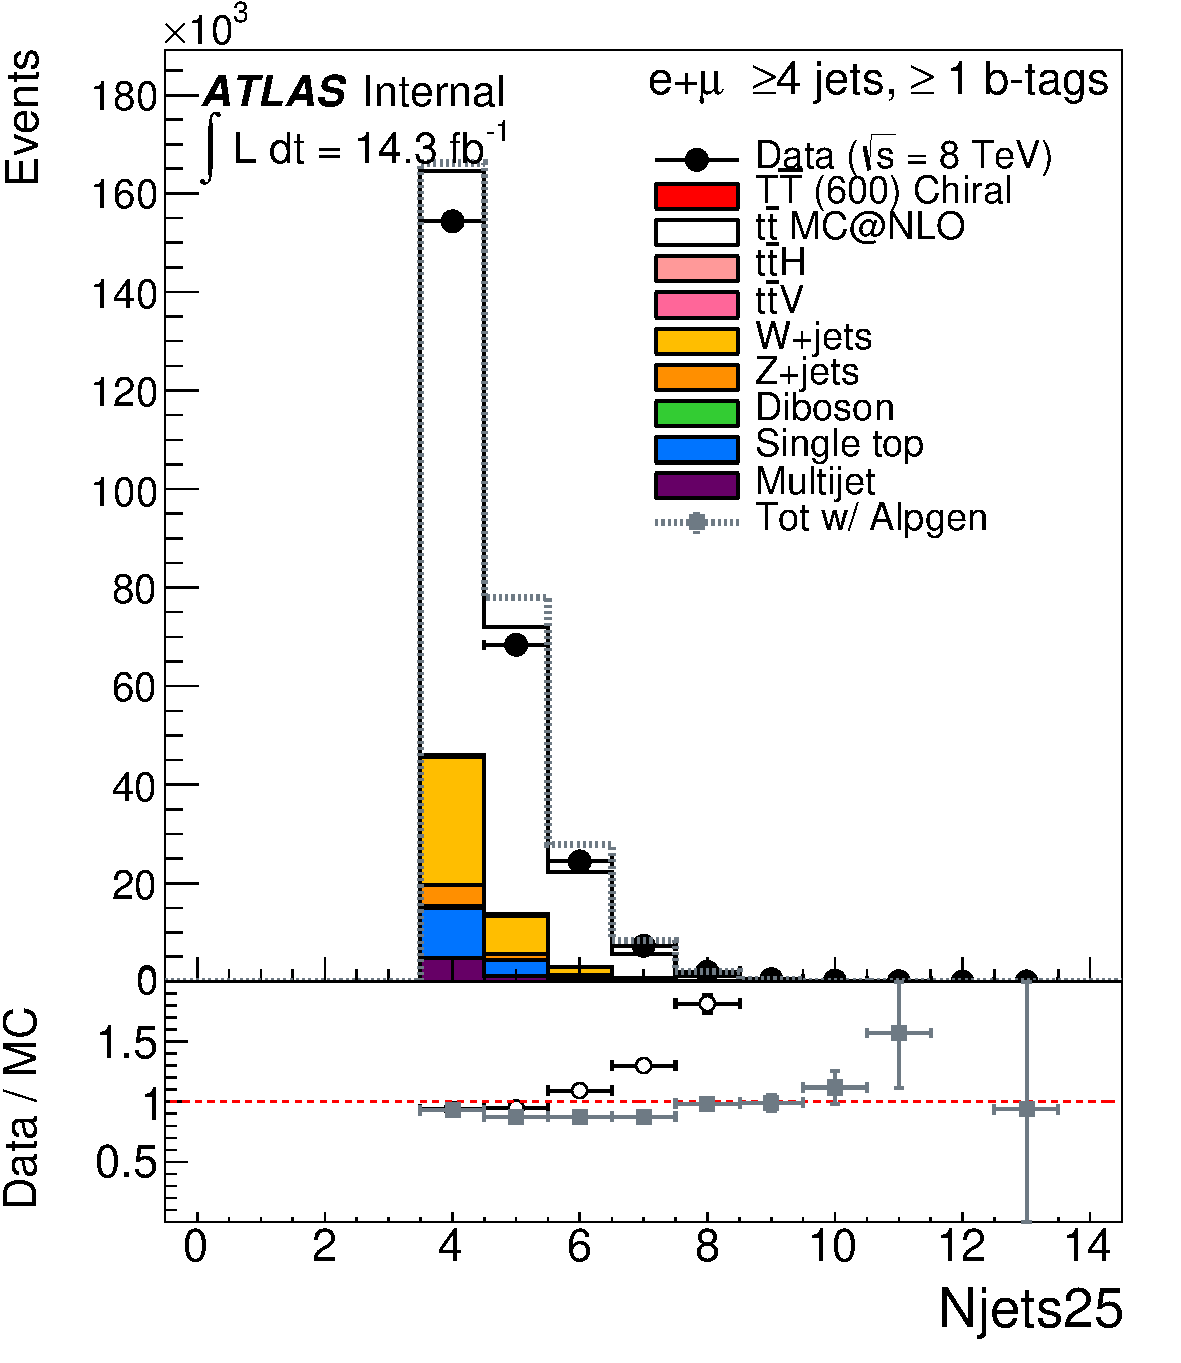
\includegraphics[width=0.32\textwidth]{vlq_analysis/figures/THESIS_c5_presel_noortho_noyields/ELEMUON/4jetin/1btagin/Njets25_ELEMUON_4jetin1btagin_NOMINAL}}
	%\subfigure[]{
  	%\includegraphics[width=0.32\textwidth]{vlq_analysis/figures/THESIS_c5_presel_noortho_noyields/ELEMUON/4jetin/1btagin/JetEta1_ELEMUON_4jetin1btagin_NOMINAL}}\\
	%\subfigure[]{
  	%\includegraphics[width=0.32\textwidth]{vlq_analysis/figures/THESIS_c5_presel_noortho_noyields/ELEMUON/4jetin/1btagin/nWhad_ELEMUON_4jetin1btagin_NOMINAL}}
	%\subfigure[]{
  	%\includegraphics[width=0.32\textwidth]{vlq_analysis/figures/THESIS_c5_presel_noortho_noyields/ELEMUON/4jetin/1btagin/Wlep_MassT_ELEMUON_4jetin1btagin_NOMINAL}}
	%\subfigure[]{
  	%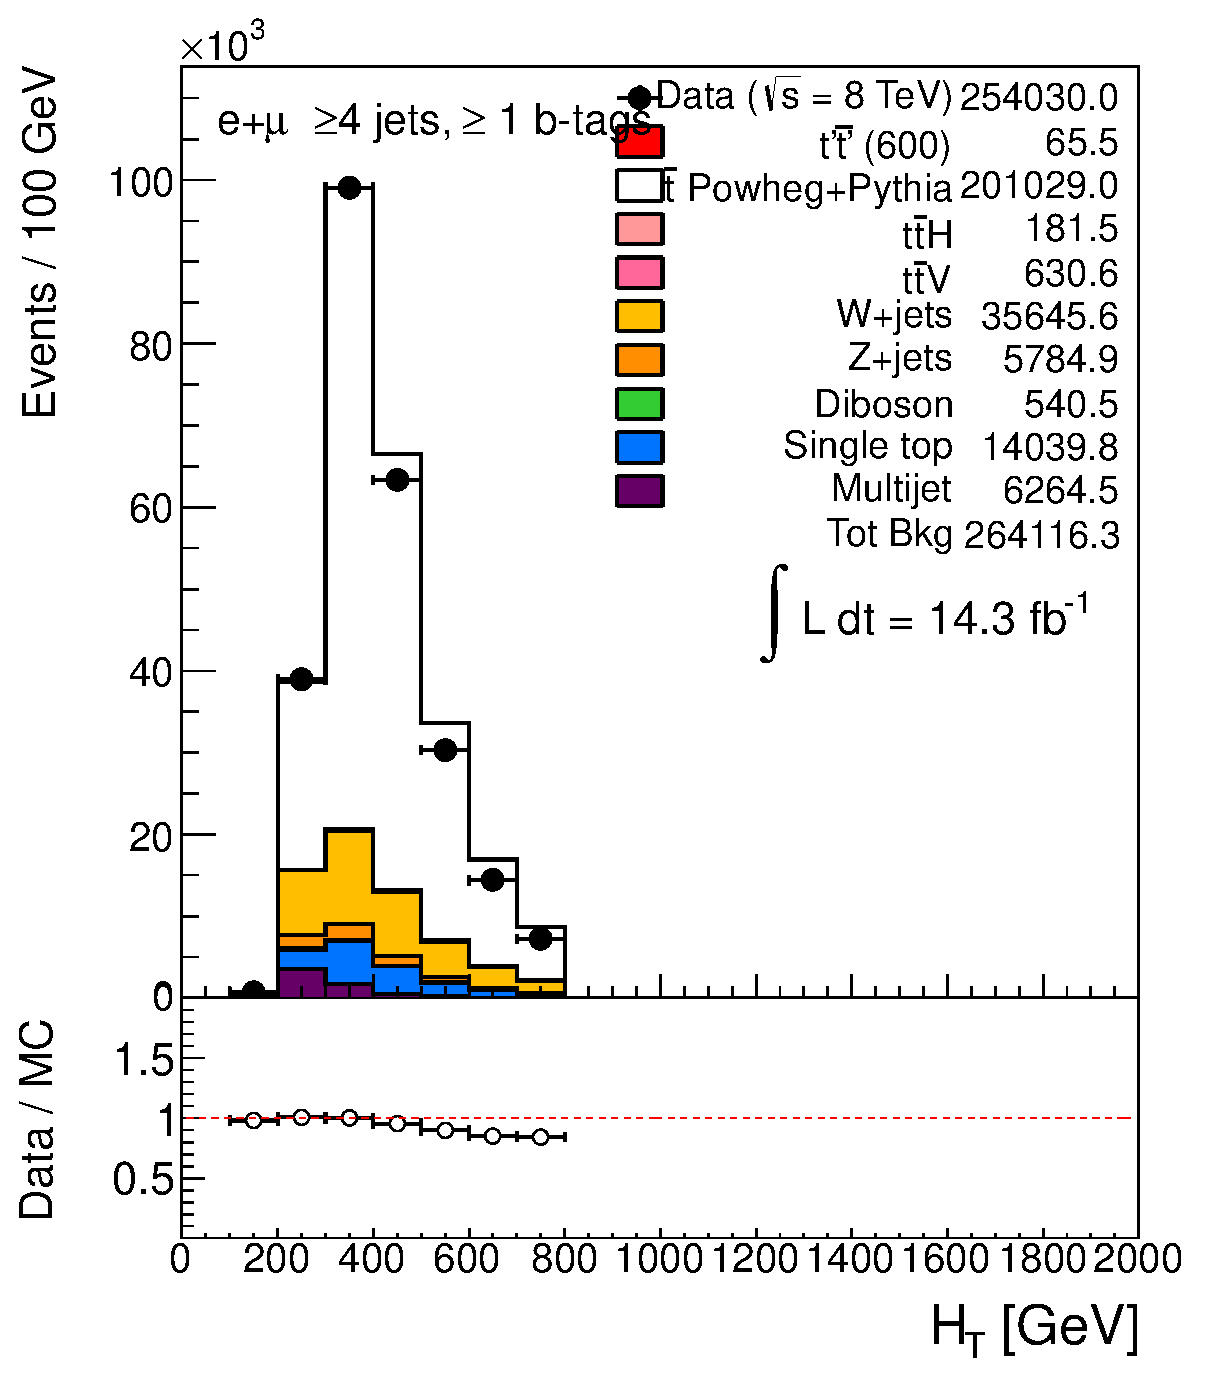
\includegraphics[width=0.32\textwidth]{vlq_analysis/figures/THESIS_c5_presel_noortho_noyields/ELEMUON/4jetin/1btagin/HTAll_ELEMUON_4jetin1btagin_NOMINAL}}
	\caption{Comparison between data and prediction plots for (a) lepton transverse momentum and
        (b) pseudorapidity, (c) missing tranverse energy, (d) transverse mass of $W$ boson, (e)
        leading jet transverse momentum, (f) number of jets with $\pt>25~\gev$.
        The selection is ``preselection'' with a blinding cut to reject signal on
        $\htfj<800\gev$. Systematic uncertainties are not shown.
        \label{fig:ELEMUON_4jetin1btagin}}
\end{center}\end{figure}



\section{Systematic uncertainties}\label{sec:systematics}

In addition to the uncertainty that comes from the stocastical nature
of events we are subject to other sources that are systematical in the sense
that they will bias the result towards a definite direction. They can come from
detector measurements, from the way we reconstruct the objects, from the Monte
Carlo modelling, and can affect either only the normalization of the total event
yield (and are called ``normalization-only'' sytematics) or also the shape 
of the distributions (and are called ``shape and normalization'' systematics).

The individual sources of systematics are treated as uncorrelated, while
the correlations eventually present in the particual systematic uncertainty are 
kept for the various processes and channels. Most of the systematic uncertainties
are common to the two analyses presented with only minor differences, e.g. in the
\htx\  analysis the systematic uncertainty affecting the jet energy scale is
split into 9 components, while it has a unique component in the \wbx\  analysis. 
The full list of systematics considered is presented in 
Table~\ref{tab:SystSummary}, labelling them as  ``normalization-only'' 
or ``shape and normalization'' systematics and indicating the number of components.

\begin{table}[htb]
\centering
\begin{tabular}{lcccc}
\toprule
Systematic uncertainty & \multicolumn{2}{c}{ \wbx\  } & \multicolumn{2}{c}{ \htx\  }\\
 & Status  & Components & Status  & Components\\
\midrule
Luminosity                  &  N & 1 &  N & 1\\
Lepton ID+reco+trigger      &  N & 1 &  N & 1\\
Jet vertex fraction efficiency & SN & 1 & SN & 1\\
Jet energy scale            & SN & 1 & SN & 8\\
Jet energy resolution       & SN & 1 & SN & 1\\
%Jet mass scale               & - & -\\
%Jet mass resolution      & - & -\\
$b$-tagging efficiency      & SN & 9 & SN & 9\\
$c$-tagging efficiency      & SN & 5 & SN & 5\\
Light jet-tagging efficiency    & SN & 1 & SN & 1\\
$t\bar{t}$ cross section    &  N & 1 &  N & 1\\
$t\bar{t}V$ cross section   &  N & 1 &  N & 1\\
$t\bar{t}H$ cross section   & - & - &  N & 1\\
Single top cross section    &  N & 1 &  N & 1\\
Dibosons cross section      &  N & 1 &  N & 1\\
$W$+jets normalization      &  N & 5 &  - & -\\
$Z$+jets normalization      &  N & 1 &  - & -\\
$V$+jets normalization      &  - & - &  N & 1\\
Multijet normalization      &  - & - &  N & 1\\
$t\bar{t}$ modelling        & SN & 3 & SN & 3\\
$V$+jets modelling         & SN & 1 &  - & -\\
$t\bar{t}$+heavy-flavour fractions &  - & -& N & 1\\
%$\TT$ modelling        & - & -\\
\bottomrule
\end{tabular}
\caption{\label{tab:SystSummary} 
List of systematic uncertainties considered in the two analyses. 
We label as ``N'' (``SN'') uncertainties taken as ``normalization-only'' 
(both ``shape'' and ``normalization'')
for all processes and channels. 
Some of the systematic uncertainties are split into more 
components for a more
accurate treatment. }
\end{table}

The systematic uncertainties are treated inside the \mclimit\ 
package~\cite{mclimitATLAS} developed for ATLAS heavy quark
searches based on the original \mclimit\ code developed
by the CDF collaboration~\cite{Heinrich:7587,Junk:8128,Junk:7904}.
Here the  histograms are interpolated between the nominal and the 
systematically shifted templates bin-by-bin, with a shift of $+0.5\sigma$
corresponding to half way between the nominal and the $+1\sigma$ shifted template.
This interpolation method is called vertical morphing and uses a linear 
bin-by-bin interpolation, but for variations below $1\sigma$ we use
quadratic interpolation to ensure a continuous derivative at zero shift.
Pseudoexperiments are generated using these interpolated numbers for
all systematic uncertainties.

Details on specific treatments of systematics in particular channels will
be given in the dedicated sections of the corresponding analysis chapters 
(Section~\ref{sec:wbxSYS} and~\ref{sec:htxSYS}).



\subsection{Luminosity}
\label{sec:syst_lumi}
The uncertainty on the absolute integrated luminosity is estimated to be
of 3.6\%~\cite{lumi}. This systematic uncertainty
is applied to all processes except the QCD multi-jet background.

\subsection{Object definitions}
\label{sec:syst_objects}
The event reconstruction introduces uncertainties on the definition of
leptons, jets and on the $b$-, $c$-, and light flavour-tagging. In the
following the related systematic uncertainties considered are described.

\subsubsection{Lepton reconstruction, identification and trigger scale factors}
\label{sec:syst_lepID}

In Sections~\ref{sec:electrons} and~\ref{sec:muons} the reconstruction
of leptons was introduced, explaining the need of adjusting the
differences between data and simulation in the efficiency for
reconstruction, identification and trigger. This is done by
applying to Monte Carlo samples some scale factors derived 
with tag-and-probe techniques 
on $Z\to \ell^+\ell^-$ ($\ell=e,\mu$) data and simulated samples.
For each of these three sources of systematic uncertainty, 
the overall systematic uncertainty is obtained 
as the quadratic sum of the statistical
and systematic uncertainties on the corresponding scale factor.

In the $e$+jets channel, the systematic uncertainties corresponding to
electron reconstruction, identification and trigger, are 0.3\%, 1.1\% 
and 0.2\%, respectively.
In the $\mu$+jets channel, the systematic uncertainties corresponding to
muon reconstruction, identification and trigger, are 0.2\%, 1.1\% and 1.4\%, 
respectively.
A total uncertainty on the signal and background acceptances of 2\% is estimated.


\subsubsection{Lepton momentum scale and resolution}

To check the accuracy of the lepton momentum scale and resolution
simulated samples of $Z\to \ell^+\ell^-$ and $J/\psi \to \ell^+\ell^-$
are used to reconstruct the particles masses (for electrons also
 $W\to e\nu$ events are used from  $E/p$  studies).
The small discrepancies observed between data and simulation are
corrected adjusting lepton energy scale and resolution in Monte Carlo
samples only for muons, while for electrons energy resolution corrections
are also applied only to Monte Carlo samples but energy scale corrections
are applied to data in all detector regions and to simulation only in 
the calorimeter transition region.
The systematic uncertainties on these scale factors are varied
separately and the result on the total yields are are at the 
sub-percent level and considered therefore ngligible in the analyses.

\subsubsection{JVF efficiency}
\label{sec:syst_jvf}

Recalling the cut applied on the JVF variable (Section~\ref{sec:jets}) 
of $|{\rm JVF}|>0.5$, the per-jet efficiency of this requirement
is estimated in $Z(\to \ell^+\ell^-)$+1-jet events both in data and
Monte Carlo simulation. Event enriched in hard-scatter jets are selected
separately from events enriched in jets from pile-up interactions and
specific efficiency and inefficiency scale factors are measured.
Scale factors for pileup jets are estimated to be consistent with 1, while
efficiency for hard-scatter jets goes from $\sim$1.03 for jets with $\pt=25\gev$
down to $\sim$1.01 for jets with $\pt>150\gev$.
An overall event weight is obtained as the product of all per-jet scale factors
and is applied to the Monte Carlo samples.
The systematic uncertainty from the propagation of the per-jet scale
factor uncertainty gives an overall uncertainty on the signal
and background acceptance of $\sim$2.5\%.


\subsubsection{Jet energy scale}
\label{sec:syst_jes}

The systematic uncertainty on the Jet Energy Scale (JES) 
has been derived combining the information from both test-beam 
and collision data and Monte Carlo
simulation~\cite{ATLASJetEnergyMeasurement, insitu5,insitu6}.  
Pile-up activity produces an additional source of systematic 
uncertainty which depends on the number of primary vertices
and on the average number of interactions per bunch crossing $<\mu>$. 
%The first estimate of the effect of pile-up on the jet energy scale uncertainty was developed in 2011~\cite{insitu6}, and subsequently validated with in situ momentum balance techniques in studies of the 2012 data.
Momentum balance techniques in $Z$+jets, $\gamma$+jets and 
multi-jet events are combined to derive a small residual correction
for jets in the transverse momentum range $20\gev<\pt<\sim1\tev$.

The overall variation due to JES systematic uncertainty 
evaluated in the central detector region 
is $\sim$4\% for jets with $\pt=25\gev$ and improves to $\sim$1\% for  
jets with $\pt=500\gev$~\cite{jesuncertainty}.
The effect of this systematic uncertainty is 
implemented in the analyses by varying in the Monte Carlo samples the 
transverse momentum of all the selected jets by $\pm$1 standard deviation.
In each event the missing transverse momentum \met\ is then corrected consistently to 
the varied $\pt$ of the jets and all the variables involving jets are also
recomputed.

As can be seen in Table~\ref{tab:SystSummary}, for the \htx\ analysis
the JES systematic uncertainty is split into 8
uncorrelated components, each with a different jet $\pt$ and $\eta$
dependence, which are treated independently.
The \wbx\ instead uses the total JES uncertainty as a single uncertainty
resulting from the sum in quadrature of all individual sources.



\subsubsection{Jet energy resolution}
\label{sec:syst_jer}

The Jet Energy Resolution (JER) was measured 
with two {\em in-situ} techniques~\cite{ATLASJetEnergyMeasurement}
as a function of the jet transverse momentum and pseudo-rapidity.
It is consistent in data and Monte Carlo simulation and no corrections
are needed.
To account for the systematic uncertainty the quadratic difference 
between the JER in data and in simulated samples is used
to smear the energy of jets in Monte Carlo simulation and a new
varied sample is obtained with a different normalisation and 
variable distributions shapes. The final result is then symmetrised
to obtain both positive and negative variations.
%In order to propagate the uncertainty in the $\pt$ resolution, for each jet in the simulation, a random number $r$ is drawn from a Gaussian distribution with mean 0 and sigma equal to the difference in quadrature between the fractional $\pt$ resolution with the tool and the nominal one.  The jet 4-momentum is then scaled by a factor $1+r$. This jet energy resolution uncertainty is assumed to be fully correlated point-by-point.
%The same rebinning algorithm as discussed in Section~\ref{sec:syst_jes} is applied.


\subsubsection{Heavy- and light-flavour tagging}
\label{sec:syst_btag}


The efficiencies in heavy flavour ($b$ and $c$) jets identification with
the $b$-tagging algorithm are measured in data and depend on the individual
jet flavour~\cite{BTaggingEfficiency,CTaggingEfficiency,LightTaggingEfficiency}.
These efficiencies are measured from data and depend on the jet flavour:
in Monte Carlo events $b$ ($c$) jet efficiencies are corrected with scale factors
of 0.9--1.0 (1.1--1.2) depending on $\pt$, light jet efficiencies are corrected 
with a  scale factor of $\sim$1.3.
Every jet in the Monte Carlo simulated events is corrected depending
on its flavour, $\pt$ and $\eta$
The uncertainty on these scale factors is 
between 7\% and 13\% for $b$ jets, between 15\% and 39\% for $c$ jets,
and $\sim$25\% for light jets.

As was reported in Table~\ref{tab:SystSummary}, the systematic uncertainty
on \btag ging (\ctag ging) efficiency is divided into nine (five) independent 
components that correspond to an eigenvector from the diagonalization of the
matrix containing the information on the total uncertainty 
per $\pt$ bin and the bin-to-bin correlations (see~\cite[Appendix P]{VHbb} for
more details).
These individual sources of systematic uncertainties 
are taken as uncorrelated between $b$, $c$ jets, and
light flavour jets. In Monte Carlo simulated events 
a per-jet weighting procedure~\cite{IFAEBtagNote}
is applied in order to propagate the \btag ging calibration
and related uncertainties.

\subsection{Theoretical cross-sections}
\label{sec:syst_bkgxsect}

Normalization-only systematic uncertainties on the theoretical
cross-sections are considered as follows:
+10\%/-11\% for the inclusive $t\bar{t}$
production cross section evaluated at approximate NNLO using 
\texttt{HATHOR}~\cite{ttbarxs}; +5\%/-4\% and $\pm 5\%$ 
for the theoretical cross sections of the single
top~\cite{stopxs,stopxs_2} and diboson~\cite{dibosonxs} backgrounds
respectively; +12\%/-17\% and  $\pm 30\%$ 
for the theoretical cross sections of the $t\bar{t}H$~\cite{lhcxs} and 
$t\bar{t}V$~\cite{ttbarVxs1,ttbarVxs2} backgrounds respectively.


\subsection{Normalizations of data-driven backgrounds and background modeling}
\label{sec:syst_norm}

Because of the differences between the effects of these systematic uncertainties
in the \wbx\ and \htx\ analyses, the reader is referred to the specific 
Sections~\ref{sec:wbxSYS} and~\ref{sec:htxSYS}


%
\section{Search for \TTbar\ pairs decaying to $Wb+X$}\label{sec:wbx}

\subsection{Boosted $W$ reconstruction}\label{subsec:boostedW}

\subsection{Control regions}\label{sec:wbxCR}

\subsection{Event selection}\label{sec:wbxEVT}

%\subsection{}\label{sec:}

%\subsection{}\label{sec:}

\subsection{Systematics}\label{sec:wbxSYS}

%
\section{Preliminary search for \TTbar\ pairs decaying to $Ht+X$}\label{sec:htx}

\subsection{Control regions}\label{sec:htxCR}

\subsection{Event selection}\label{sec:htxEVT}

%\subsection{}\label{sec:}

%\subsection{}\label{sec:}

\subsection{Systematics}\label{sec:htxSYS}



\section{Statistical analysis}\label{sec:cls}

To test the presence or absence of signals from new physics we use the
\cls{s}\ method~\cite{cls,cls_2} originally developed in the context of Higgs
searches at the LEP collider~\cite{Read:451614}.
The fundamental principle of this technique is that, in order to 
exclude or verify a theory predicting some kind of signal over some other kind
of background, both ``background only'' and ``signal plus background''
hypotheses have to be tested. Once a test statistic $Q$ has been chosen
analysis-wise, two confidence levels (CL) are defined for the two hypotheses:
\begin{eqnarray}\label{eq:clbclsb}
\cls{b} &=& P(Q \leq Q_{\rm obs}|\mathcal{H}_{b}),\\
\cls{s+b} &=& P(Q \leq Q_{\rm obs}|\mathcal{H}_{s+b}),
\end{eqnarray}
with $Q_{\rm obs}$ being the observed value in data of the 
test statistic. It is good to identify well separated test statistic
distributions in order to be able to clearly distinguish between 
events consistent with the backgroud only prediction and events
showing deviations consistent with the signal+background hypothesis.

The \cls{s}\ is then defined as the ratio of the two:
\begin{equation}\label{eq:cls}
\cls{s} = \cls{s+b}/\cls{b}
\end{equation}
and its meaning is given by its relation with the confidence 
level $CL$ for the exclusion of the signal hypothesis 
$(1 - \cls{s}) \leq CL$.
%i.e. values of $\cls{s}<0.05$ 
Similarly, the confidence level for excluding the background only
hypothesis is the $p$-value $1 - \cls{b}$ and the value required to claim 
discovery is of $\sim 10^{-7}$. The motivation that led to
the definition of \cls{s} instead of using \cls{s+b}, which also
corresponds to the confidence level in excluding the signal+background
hypothesis, is that the latter might wrongly exclude scenarios to
which the analysis is simply not sensitive to like is the general case
for searches for rare events.

\begin{figure}[htb]\begin{center}
        \psfrag{AAA}{\tiny $P(f(Q)|\mathcal{H}_{b})$}
        \psfrag{BBB}{\tiny $P(f(Q)|\mathcal{H}_{s+b})$}
        \psfrag{CCC}{\tiny $1 - CL_{b}$}
        \psfrag{DDD}{\tiny $CL_{s+b}$}
        \psfrag{XXX}{$f(Q)$}
        \psfrag{YYY}{\hskip-10ex Probability density}
	\subfigure[]{\label{fig:sepLLR}
  	\includegraphics[width=0.45\textwidth]{vlq_analysis/figures/separatedLLR}}
	\subfigure[]{\label{fig:ovrLLR}
  	\includegraphics[width=0.45\textwidth]{vlq_analysis/figures/overlappedLLR}}
	\caption{Example of (a) sensitive and (b) not sensitive analyses using the test 
        statistics $f(Q)$, often chosen as $-2\log Q$.}
\end{center}\end{figure}


For the two analyses presented in this dissertation, the test statistic
is defined as a log-likelihood ratio 
\begin{equation}\label{eq:llr}
LLR = -2\log \dfrac{\mathcal{L}({\rm data}|\mathcal{H}_{s+b})}{\mathcal{L}({\rm data}|\mathcal{H}_{b})},
\end{equation}
where the likelihoods $\mathcal{L}({\rm data}|\mathcal{H}_{s+b})$
 and $\mathcal{L}({\rm data}|\mathcal{H}_{b})$ for 
signal+background and background only hypothesis
are built from the chosen discriminant variable distribution 
as the bin by bin product of Poisson probabilities to observe the
data under one or the other hypothesis.
Eventually more than one channel can be combined (like will be
the case in the \htx\ analysis) and the complete formula for
the likelihood computation reads:
\begin{align}
-2 \log {\cal L}({\rm data}|\mathcal{H}_x) 
   & =  
   %=
   -2 \log {\cal L}(\vec{n}|R,\vec{s},\vec{b},\vec{\theta}) \notag\\
   %=
   & =  
  -2 \sum_{i=1}^{N_{chan}}\sum_{j=1}^{N_{bins}} (n_{ij}\log \mu_{ij}-\mu_{ij})+\sum_{k=1}^{N_{par}} \theta_k^2.
\end{align}
Here the first sum is over the number of channels
combined in the analysis $N_{chan}\geq 1$ and the 
second sum is over the number of the discriminant variable
histogram bins $N_{bins}$. $n_{ij}$ ($\mu_{ij}$) is the 
number of events in data (expected number of events) 
for channel $i$ and histogram bin $j$. $\mu_{ij}$ is given by
$\mu_{ij} = R s_{ij}(\vec{\theta})+ b_{ij}(\vec{\theta})$, 
where $s_{ij}$  and $b_{ij}$ represent the
expected signal and background yields, 
the first being equal to zero in the background only hypothesis.
$R$ is a scaling 
parameter applied to the signal
to test the sensitivity of the search and $\vec{\theta}$
are the nuisance parameters parametrizing the effect of
systematic uncertainties. 
The statistical uncertainty of the Monte Carlo samples is 
also taken into account when computing our likelihoods as
an uncertainty of the templates, which in the case of
the non-$t\bar{t}$ background are merged into a single
template  with different weights.
%The {\sc mclimit} flag used is 2, meaning we consider the uncertainties as given by the uncertainties of the templates. 
%This allows us to correctly estimate the statistical uncertainty when many templates are merged together with different weights, such as in the case of the merged non-$t\bar{t}$ background.
%These parameters are assigned Gaussian penalty terms in the likelihood corresponding
%to their nominal uncertainties.
For both hypotheses pseudoexperiments are generated to
account in each bin for statistical fluctuations (Poisson-distributed)
and systematic variations (Gaussian-distributed). The effect of
systematic uncertainties are described by nuisance parameters taken
at their nominal values and no parameter fitting is performed.
In the case of the \htx\ analysis it will be explained that
two additional nuisance parameters are introduced and fitted
to help costraining the sensitivity degradation due to a poor
Monte Carlo modeling of \ttbar\ heavy flavor component.

In absence of data excess over background prediction, values of
$\cls{s}<0.05$ are considered to exclude a signal cross section
at 95\% CL.



\clearpage{\pagestyle{empty}\cleardoublepage}
\clearpage{\pagestyle{empty}\cleardoublepage}

\chapter{Preliminary search for $T\bar{T}\to Wb+X$}\label{chap:wbx}


\clearpage{\pagestyle{empty}\cleardoublepage}
\clearpage{\pagestyle{empty}\cleardoublepage}

\chapter{Preliminary search  for \TTbar\ pairs decaying to $Ht+X$}\label{chap:htx}

\section{Control regions}\label{sec:htxCR}

\section{Event selection}\label{sec:htxEVT}

%\section{}\label{sec:}

%\section{}\label{sec:}

\section{Systematics}\label{sec:htxSYS}



%%%%NB COPY PASTE
The total prior systematic uncertainty
in the background normalisation in the $\geq 4$ $b$-tags channel is 
$\sim$42\%, with the dominant uncertainties being from $b$ tagging efficiency (16\%),
$c$ tagging efficiency (11\%), jet energy scale (11\%), $t\bar{t}$ modelling (11\%), 
$t\bar{t}$+heavy-flavour fractions (32\%) and $t\bar{t}$ cross section (10\%).
As a result of the two-parameter fit, the total background uncertainty is reduced 
by about 80\% in this channel. The total  systematic uncertainty
in the signal normalisation in the $\geq 4$ $b$-tags channel is 
$\sim$21\%, completely dominated by the uncertainty in the $b$ tagging efficiency.


\clearpage{\pagestyle{empty}\cleardoublepage}
\clearpage{\pagestyle{empty}\cleardoublepage}

\chapter{Combined results}\label{chap:results}

Through Chapters~\ref{chap:vlq},~\ref{chap:wbx} and~\ref{chap:htx}
we presented the strategy adopted for the searches of vector-like
top partners in the single lepton channel and implemented into
two complementary analyses: the \wbx\ and the \htx\ analyses.
Each of these analyses is probing a different
area of the two-dimensional plane (described in Section~\ref{sec:strategy}) 
defined in order to perform
a model-independent scan of the three possible decay channels branching ratio 
mixing phase space.
In this chapter we are going to illustrate how the results
obtained by the individual analyses (Sections~\ref{sec:wbxRES} 
and~\ref{sec:htxRES}) perform when the search channels are
combined (Section~\ref{sec:results_comb}).
In Section~\ref{sec:coverage} we compare
the coverage of the branching ratios two-dimensional
mixing plane by the four quasi-model independent
searches for vector-like quarks performed
by the Exotics group.


\section{Combination of the \wbx\ and \htx\ analyses}\label{sec:results_comb}

As the \wbx\ and the \htx\ analyses do not overlap
thanks to the orthogonality requirements (rejection of
events with $\geq$ 6 jets and $\geq$ 3 \btag ged jets
in the \wbx\ analysis, rejection of events with $H_T>700~\gev$
in the \chii\ channel of the \htx\ analysis), it is possible
to obtain a fully combined result. Figure~\ref{fig:searchchan}
reports the final search channels to be used.

\begin{figure}[h!tb]\begin{center}
	\subfigure[]{\label{fig:htx2}
%\includegraphics[width=0.45\textwidth]{htx_analysis_14ifb/figures/final/HTAll_6jetin2btagex_ELEMUON.eps}}
\includegraphics[width=0.45\textwidth]{results/figures/THESIS_c8_signal/HTAll_6jetin2btagex_ELEMUON.eps}}
	\subfigure[]{\label{fig:htx3}
%\includegraphics[width=0.45\textwidth]{htx_analysis_14ifb/figures/final/HTAll_6jetin3btagex_ELEMUON.eps}}
\includegraphics[width=0.45\textwidth]{results/figures/THESIS_c8_signal/HTAll_6jetin3btagex_ELEMUON.eps}}
	\subfigure[]{\label{fig:htx4}
%\includegraphics[width=0.45\textwidth]{htx_analysis_14ifb/figures/final/HTAll_6jetin4btagin_ELEMUON.eps}}
\includegraphics[width=0.45\textwidth]{results/figures/THESIS_c8_signal/HTAll_6jetin4btagin_ELEMUON.eps}}
	\subfigure[]{\label{fig:wbx1}
%\includegraphics[width=0.45\textwidth]{wbx_analysis_14ifb/figures/confnoteplots/VLQAna_WbX_1W_MWb_4_ELEMUON_cutflow1234567_NOMINAL.eps}}
\includegraphics[width=0.45\textwidth]{results/figures/THESIS_c8_signal/VLQAna_WbX_1W_MWb_4_ELEMUON_cutflow1234567_NOMINAL.eps}}
	\caption{Final discriminant variables distributions in the search channels
        of the \htx\ analysis ($\HT$ in (a) \chii, (b) \chiii\ and (c) \chiv\ channels)
        and of the \wbx\ analysis (\mreco\ in the \tight\ channel). In all plots the
        signal is shown for the singlet model. The uncertainty bands include statistical 
        and systematic uncertainties.\label{fig:searchchan}}
\end{center}\end{figure}

For the purpose of a combined statistical analysis
of the four channels,
choices on the systematic 
uncertainties treatment have to be done.
Uncertainties that are common to both analyses and that
are treated in the same way are considered as fully 
correlated and are: integrated luminosity; lepton reconstruction, 
identification and trigger (1 component); jet vertex fraction;
jet energy resolution;
$b$ tagging (9 components); $c$ tagging (5 components); light-jet 
tagging (1 component);
background cross sections ($t\bar{t}$, single top, diboson, $t\bar{t}V$).
For the JES uncertainty, while the \wbx\ analysis considers a single component
the \htx\ uses the 8 components breakdown and is then impossible to 
correlate the individual JES uncertainty sources one by one.
Since in the \htx\ analysis the dominant JES uncertainty eigenvector is the BASELINE
(see Section~\ref{sec:htxSYS}) the choice is to correlate the \wbx\ analysis JES 
uncertainty with the BASELINE uncertainty of the \htx\ analysis.
The systematic uncertainties that are not taken as correlated are:
$W$+jets normalization, divided into 5 components in the \wbx\ 
analysis and only 1 in the \htx\ analysis where, however, is a negligible 
background; $t\bar{t}$ modeling, as the two analyses use different $t\bar{t}$ 
Monte Carlo generators and probe very different
final state kinematics region with different flavor composition.

The benchmark model chosen to show the exclusion limit as a function
of the mass is the vector-like singlet $T$ quark scenario, as
it is the common benchmark model for the two analyses. In this
case the \htx\ analysis performed better than the \wbx\ analysis,
giving an  observed (expected) 95\%  CL  limit value of
$m_{\T}>640\,(615)\gev$.
Figure~\ref{fig:limits1D_combo} shows the observed and expected 
upper limits on the \TTbar\ production cross section 
times branching fraction as a function of $m_{\T}$ for a weak-isospin
singlet  after combination of the two analyses.
The observed (expected) 95\% CL limit is 
$m_{\T}>670\,(675)\gev$ for the central value 
of the theoretical cross section,
improving by $\sim$30$\gev$ the expected sensitivity 
obtained by the \htx\ analysis alone.

\begin{figure}[h!tb]
\centering
\includegraphics[width=0.6\textwidth]{results/figures/lim_singlet_comb.eps} 
\caption[bla]{Observed (solid line) and expected (dashed line) 95\% CL upper limit on the $\T \bar{\T}$ cross section times branching fraction
for a vector-like singlet $\T$ quark  as a function of the $\T$ quark mass, resulting from the combination of
the \wbx\ and the \htx\ analyses.
The surrounding shaded bands correspond to the $\pm1$ and $\pm2$ standard deviations around the expected limit. 
The thin red line and band show the theoretical prediction and its $\pm1$ standard deviation uncertainty.

\label{fig:limits1D_combo}}
\end{figure}

Figure~\ref{fig:limits2D_combo} shows the two-dimensional branching ratio plane for 
different values of $m_{\T}$ with the  resulting 95\% CL exclusion limits.
Comparing this result with the ones of Figures~\ref{fig:limits2D_wbx} 
and~\ref{fig:limits2D_htx} it is evident the improvement resulting
from the combination of the two analyses, covering a much larger
area than the simple addition of two individual ones.
From this picture, vector-like top partners are completely excluded
no matter of the model in the mass range from 350~\gev\ up to 550~\gev\ 
(almost up to 600~\gev).

\begin{figure}[h!bt]
\centering
\includegraphics[width=0.9\textwidth]{results/figures/lim_Scan2D_comb.eps}
\caption{
Observed (red filled area) and expected (red dashed line) 95\% CL exclusion in the plane of
$BR(\T \to Wb)$ versus $BR(\T \to Ht)$, for different values of the vector-like $\T$ quark mass.
The grey (dark shaded) area corresponds to the unphysical region where the sum of branching ratios exceeds unity. 
The default branching ratio values from the \texttt{PROTOS} event generator for the weak-isospin singlet and doublet cases 
are shown as plain circle and star symbols, respectively. This result  from the combination of
the \wbx\ and \htx\ analyses includes both statistical and systematic uncertainties.
\label{fig:limits2D_combo}}
\end{figure}

It is interesting to compare the 
combined result
of the \wbx\ and \htx\ analyses
of Figure~\ref{fig:limits2D_combo} 
with the separate analysis results
to understand the impact on sensitivity
of the statistical combination of
the search channels.
This comparison is presented in 
Figure~\ref{fig:limits2D_potentialcombo},
where the combined result is overlapped
to the two separate results in the branching ratio
plane.
Looking e.g. at the 650~\gev\ mass point,
it can be clearly seen how the singlet
scenario, lying outside of the expected exclusion
region in the case of the single \htx\ analysis,
falls within the excluded area when
the same analysis is combined with the
\wbx\ analysis, which by itself does not 
have exclusion sensitivity to such benchmark point.


\begin{figure}[h!bt]
\centering
\includegraphics[width=0.9\textwidth]{results/figures/combinationoverlap.eps}
\caption{
Observed (filled area) and expected (dashed line) 95\% CL exclusion in the plane of
$BR(\T \to Wb)$ versus $BR(\T \to Ht)$, for different values of the $\T$ quark mass,
as result of the \wbx\ analysis (green), \htx\ analysis (blue), and the combination of the two (yellow).
The grey (dark shaded) area corresponds to the unphysical region where the sum of branching ratios exceeds unity. 
The default branching ratio values from the \texttt{PROTOS} event generator for the weak-isospin singlet and doublet cases 
are shown as plain circle and star symbols, respectively. All results
include both statistical and systematic uncertainties.
\label{fig:limits2D_potentialcombo}}
\end{figure}

\section{Comparison to other searches}\label{sec:coverage}

As briefly introduced in Section~\ref{sec:strategy}, two
additional analyses have been performed on the same dataset
as the \wbx\ and \htx\ analyses to search for heavy vector-like
top and bottom quarks in final states with exactly two leptons:
a search in the same-sign 
dilepton channel~\cite{ATLAS-CONF-2013-051} and 
a search in the opposite-charge dilepton channel~\cite{ATLAS-CONF-2013-056}.
It was shown that the four analyses probe different 
regions of the 2-dimensional mixing plane and are,
hence, complementary. Even though the single lepton and
the dilepton channels should have very little overlap,
it was not possible to ensure a complete
orthogonality between all the analyses and they have
not, therefore, been combined\footnote{This
fact is mainly due to the different timescales
and frameworks at which the analyses have been developed. 
The \wbx\ and \htx\ searches
have been conceived to be combined since the
early stages of their design and were performed
inside the same analysis framework.}.
It is however useful to visualize how
the four searches contribute to the full
coverage of the branching ratios mixing plane by
observing Figure~\ref{fig:limits2D_allcombo}.
Here the results from the four searches,
each obtained independentely, are simply
overlapped. This picture corresponds somehow to
a ``worst case scenario'' of a possible
real combination of the four searches, as
in general the statistical analysis in the
case of additional signal enriched
channels would gain sensitivity. 
This can easily be grasped when looking
at the comparison between the combined result
of the \wbx\ and \htx\ analyses
with the plain overlap of the separate
coverages, shown in the previous section 
in Figure~\ref{fig:limits2D_potentialcombo}.

Figure~\ref{fig:limits2D_allcombo} shows that already
without combining any of the four searches,
\T\ quarks with masses up to 550~\gev, almost up
to 600~\gev, are excluded at 95\% CL without 
any assumption on the model. The same kind of
picture has been obtained in the branching ratio plane for
\B\ quarks, shown in Figure~\ref{fig:limits2D_allvlb}.
Here the analyses contributing to the
95\% CL exclusion in the BR($B\to Hb$) vs  BR($B\to Wt$)
plane are the two searches in the multilepton channel.
The absence of a search probing the top-left corner
of the branching ratio plane leaves for \B\ masses from 400~\gev up to
600~\gev only a very small area uncovered.


\begin{landscape}
\begin{figure}[h!bt]
\centering
\includegraphics[width=1.5\textwidth]{results/figures/ATLAS_VLQ_TT_june2013_step4.eps}
\caption{
Observed (filled area) and expected (dashed line) 95\% CL exclusion in the plane of
$BR(\T \to Wb)$ versus $BR(\T \to Ht)$, for different values of the $\T$ quark mass.
In blue is shown the area excluded by the single lepton \htx\ analysis;
in orange is shown the area excluded by the same-sign dilepton analysis;
in red is shown the area excluded by the opposite-sign dilepton $\TTbar\to Zt+X$ analysis;
in green is shown the area excluded by the single lepton \wbx\ analysis.
The grey (dark shaded) area corresponds to the unphysical region where the sum of branching ratios exceeds unity. 
The default branching ratio values from the \texttt{PROTOS} event generator for the weak-isospin singlet and doublet cases 
are shown as plain circle and star symbols, respectively. This result includes both statistical and systematic uncertainties.
\label{fig:limits2D_allcombo}}
\end{figure}
\end{landscape}


\begin{landscape}
\begin{figure}[h!bt]
\centering
\includegraphics[width=1.5\textwidth]{results/figures/ATLAS_VLQ_BB_june2013_step2.eps}
\caption{
Observed (filled area) and expected (dashed line) 95\% CL exclusion in the plane of
$BR(\B \to Wt)$ versus $BR(\B \to Hb)$, for different values of the $\B$ quark mass.
In orange is shown the area excluded by the same-sign dilepton analysis;
in red is shown the area excluded by the opposite-sign dilepton $\TTbar\to Zt+X$ analysis.
The grey (dark shaded) area corresponds to the unphysical region where the sum of branching ratios exceeds unity. 
The default branching ratio values from the \texttt{PROTOS} event generator for the weak-isospin singlet and doublet cases 
are shown as plain circle and star symbols, respectively. This result includes both statistical and systematic uncertainties.
\label{fig:limits2D_allvlb}}
\end{figure}
\end{landscape}



\section{Outlook}\label{sec:combOUT}

At the time this dissertation is being
written, all of the four searches for
vector-like quarks are being updated to
the full available statistics of
pp collisions at \rts=8~\tev, about 20~\ifb,
for publication. The four searches maintain the
core strategies but have improvements in
background modeling (in particular with better
and more statistically populated Monte Carlo samples)
and reduced systematic uncertainties.
Searches in new channels are being developed, namely
$B\to Wt+X$ and $B\to Hb+X$, thus allowing for
the full coverage of the branching ratio plane.
The complete plan for vector-like quark searches
in ATLAS is to combine all these analyses to 
achieve the highest possible sensitivity.


\clearpage{\pagestyle{empty}\cleardoublepage}

\phantomsection
\addcontentsline{toc}{chapter}{Conclusions}
\clearpage{\pagestyle{empty}\cleardoublepage}

\chapter*{Conclusions and outlook}\label{chap:conclusions}

\vskip-1.5cm

Two quasi-model independent searches for 
pair production of vector-like top partners 
in proton-proton collisions at a \cme\ of 8~\tev\ 
have been presented in this dissertation. The final states considered
for both analyses involve one lepton and many jets but different
strategies are adopted in order to achieve sensitivities in different
corners of the decay phase space. Indeed, a peculiar fact for these
searches that has been stressed many times over these pages is the 
unpredicted nature of the heavy vector-like top partners model. 
As a direct consequence, the two analyses have been designed
and developed to be optimized for a particular decay mode and
to have orthogonal channels in order to allow
for a combined search that could exploit the specific sensitivities.

Three particular models, interesting from a theoretical point
of view (but not for this more favoured than others), are considered
over the two analyses: the chiral fourth-generation, with 
BR$(T\to Wb)=1$ for any value of the heavy quark mass; 
the singlet vector-like, with BR$(T\to Wb)\sim 0.5$ and 
BR$(T\to Ht)\sim 0.3$ for almost all
values of the heavy quark mass considered in the searches;
the doublet vector-like, with BR$(T\to Wb)= 0$ and 
BR$(T\to Ht)\in$ [0.50, 0.75] for all the values of the heavy quark mass.
In the \wbx\ analysis, it was possible to exclude at a 95\% CL
pair-produced chiral fourth-generation top partners and vector-like
$Y$ quarks with masses up to 740~\gev, and pair-produced vector-like 
singlet top partners with  masses up to 505~\gev.
In the \htx\ analysis, it was possible to exclude at a 95\% CL
pair-produced vector-like singlet and doublet top partners with 
masses up to 640~\gev\ and 790~\gev\ respectively.
When the two analyses are combined, the observed exclusion limit
for the only model where both analyses are sensitive, the
vector-like singlet $T$, is pushed $\sim$30~\gev\ further the
best result of the two, obtained by the \htx\ analysis,
achieving a 95\% CL exclusion of pair-produced vector-like singlet 
top partners with masses up to 670~\gev. While this might not
look like a significant improvement, the power of the combination
of the two searches is evident looking at the coverage of the
two-dimensional branching ratio plane, where  95\% CL exclusion is set for
pair-produced vector-like top partners with masses up to 550~\gev\ 
independently from the model, and also the plane for the 600~\gev\ mass
point is almost fully excluded. This strongly encourages to perform,
in the future, full combination of searches for vector-like quarks.

The mass range excluded at 95\% CL up to now
is getting closer and closer to the point where pair-production
of vector-like quarks will start to be disfavoured with respect
to single production. In this sense, while it is desirable to continue to
exploit the experience achieved up to now with the searches for
pair-produced vector-like quarks in the single lepton and multi-lepton
channels, it is a good idea to start designing searches for
single-produced vector-like quarks for LHC Phase-II.
Further improvements are possible for the searches
presented in this dissertation without changing the core of
the analysis strategies. During Phase-II they will benefit
of the increased \cme\ available for heavy quark production
in pp collisions with \rts=14~\tev\ and of the high integrated
luminosity (100~\ifb\ of data are expected over three years
of operation). With high luminosity comes the challenge of
dealing with higher pile-up, but considering that vector-like
quark searches involve high-\pt\ objects this should not
represent a major issue.

Besides the great discovery potential, the combination
of multiple searches will provide useful insights on the
exotic quark properties, like their quantum numbers or
the measurement of their branching ratios. 
Adding searches for single production of vector-like quarks
would also allow to measure the electroweak couplings of
these particles with the Standard Model quarks from the third generation.
Finally, these searches are even more interesting since
they will probe a wide range of
signatures that are often shared with other new physics
scenarios. Given the fact that during these last successful years
of LHC operation no hints on what lies ``beyond the Standard Model''
have emerged, the winning strategy is for sure not to confine ourselves 
to exclusive models.


\clearpage{\pagestyle{empty}\cleardoublepage}

\appendix


\clearpage{\pagestyle{empty}\cleardoublepage}

\chapter{The Tag Rate Function method}\label{app:trf}

When requiring high \btag ged jet multiplicity in an analysis, 
usually the available statistics in Monte Carlo simulated  samples 
is significantly reduced. This leads to large fluctuations
for the final discriminant variable distribution
and, as a direct consequence, reduced sensitivity of
the search because of unphysical variations of 
the systematic uncertainties affected by the unreliable
statistical uncertainties.
Furthermore this can introduce a bias in the observed limits
depending on the side of the fluctuation of the Monte Carlo
templates with respect to the data in the final signal region.
A Tag Rate Function (TRF) method can mitigate this problem
by keeping the full Monte Carlo pre-tag statistics and deriving
the shape and normalization predictions in the \btag ged channels
through a reweighting procedure.

While the vector-like signal samples, obtained using a fast simulation
of the detector, have enough statistics in the final channels for
both the \wbx\ and \htx\ analyses, Monte Carlo backgrounds are highly
affected by the cuts specifically designed to reduce their presence
in the final selection.
Therefore, the TRF method is applied to all Monte Carlo samples in
the \htx\ analysis, which requires high \btag ged jet multiplicities
in its search channels, and to all non-\ttbar\ Monte Carlo samples
($W$+jets, $Z$+jets, diboson, single-top, $\ttbar V$) in the \wbx\ 
analysis, which requires only one \btag ged jet but drastically
reduces the background contribution to the signal region through
tight requirements.

In this appendix the principle of this method and the various 
studies performed to validate its usage in the analyses
are discussed.



\section{TRF method principle}

When a direct cut on the
\btag ging weight returned by the \btag ging algorithm
is applied, events that do not have the requested number
of jets satisfying this cut are rejected. Considering that
commonly chosen working points for the \btag ging algorithms
have a measured efficiency of 70\%, it is easy to imagine the
potential loss in acceptance when requiring more that one
\btag ged jets.
By using the TRF method, no event is cut based on how many
$b$-taged jets are counted, but instead all the pre-tag events 
are reweighted.
The event weight is calculated using the
per-jet  \btag ging efficiency
(which depends on the jet's $\pt$, $\eta$ and true jet flavour)
and based on the kinematics and flavour of the 
jets found in each event.
This weight can be interpreted as the probability of the 
given event to contain the desired number of \btag ged jets. 

Given a jet with $\pt$, $\eta$ and flavour $f$, its 
tagging probability can be written as:
\begin{equation}
	\varepsilon \left(\pt,|\eta|,f\right).
\end{equation}

For instance, for a given event with $N$ jets, the probability of 
containing exactly one $b$-tagged jet can be computed as:
\begin{align}
	P_{=1} &= \sum\limits_{i=1}^N \left( \varepsilon_{i} \prod\limits_{j \neq i} \left( 1 - \varepsilon_{j} \right) \right).\end{align}
This can be generalized as the probability of containing exactly $M$
$b$-tagged jets by iterating over all the possible subsets of $M$ and $N-M$
jets as:
\begin{align}
        P_{=M} &= \sum\limits_{i,\dots,m=1}^N 
        \left( 
        \prod\limits_{i=1}^{m=M} \varepsilon_{i}  
        \prod\limits_{j=m+1}^N \left( 1 - \varepsilon_{j} \right) 
        \right),
	%P_{=m} &= \sum\limits_{i,j,\dots,m=1}^N \left( \varepsilon_{i}\varepsilon_{j}\dots\varepsilon_{m}(1-\delta(i,j,\dots,m)) \prod\limits_{k \neq i\neq j \dots\neq m} \left( 1 - \varepsilon_{k} \right) \right), \\
\end{align}
and in general the probability for inclusive $b$-tagging selections can be
computed:
\begin{align}
	P_{=0} &= \prod\limits_{i=1}^N \left( 1 - \varepsilon_{j} \right), \\
	P_{\geq 1} &= 1 - P_{=0},\\
&\dots \notag\\
	P_{\geq m} &= 1 - \sum\limits_{i=0}^{m-1} P_{=i}.
\end{align}

\subsection{Validation}
This method relies on the correct calibration of the \btag ging efficiency in 
Monte Carlo samples. 
Closure tests performed with the official calibration files have shown that 
the efficiency parametrization is not as accurate as expected.
Assuming a correct calibration, the average of the histogram of 
$1/\varepsilon$ vs $\eta$, $\pt$ and true jet flavour should be 
flat and with mean equal to one.

In Figure~\ref{fig:closure} the result of this test is shown, and it 
can be observed that for the official maps (the left colums) there 
are departures from closure of to up to 40\% in some regions of the light flavor
map, and on average of 13\%.
New efficiency maps have been derived using a combination 
of $t\bar{t}$ \texttt{MC@NLO}, $t\bar{t}$ \texttt{Alpgen}, and 
\texttt{Protos} $\TT$ Monte Carlo samples.
The plots on the right column of Figure~\ref{fig:closure} 
show reasonably good closure for the newly derived efficiency map,
which will therefore be used for the probability computations in the TRF method.

\begin{figure}[h!tb]\begin{center}
	\subfigure[]{
    \includegraphics[width=0.45\textwidth]{appendices/figures/trf/5closureRebin.eps}}
	\subfigure[]{
    \includegraphics[width=0.45\textwidth]{appendices/figures/trf/5myclosureRebin.eps}}
	\subfigure[]{
    \includegraphics[width=0.45\textwidth]{appendices/figures/trf/4closureRebin.eps}}
	\subfigure[]{
    \includegraphics[width=0.45\textwidth]{appendices/figures/trf/4myclosureRebin.eps}}
	\subfigure[]{
    \includegraphics[width=0.45\textwidth]{appendices/figures/trf/0closureRebin.eps}}
	\subfigure[]{
    \includegraphics[width=0.45\textwidth]{appendices/figures/trf/0myclosureRebin.eps}}
	\caption{Results of the closure test using efficiency from the official calibration file (left column) and the private efficiency map (right column). The test is split in the different jet flavours: $b$-jets (top), $c$-jets (middle) and light jets (bottom).\label{fig:closure}}
\end{center}\end{figure}

As a validation check, Figure~\ref{fig:btags} compares the spectrum
of the number of \btag ged jets distribution in the  $t\bar{t}$ Monte Carlo
sample simulated with \texttt{ALPGEN} obtained using the TRF method
and the direct \btag ging. The shapes are found to be compatible.

\begin{figure}[h!tb]\begin{center}
	\subfigure[]{\label{fig:trf4j}
    \includegraphics[width=0.32\textwidth]{appendices/figures/trf/ttbarAlpgen_HFOR_ntags_4jetex.eps}}
	\subfigure[]{\label{fig:trf5j}
    \includegraphics[width=0.32\textwidth]{appendices/figures/trf/ttbarAlpgen_HFOR_ntags_5jetex.eps}}
	\subfigure[]{\label{fig:trf6j}
    \includegraphics[width=0.32\textwidth]{appendices/figures/trf/ttbarAlpgen_HFOR_ntags_6jetin.eps}}
	\caption{Comparison of the TRF and direct $b$-tag cut prediction for the $b$-tag spectrum, in the 4 jet exclusive (a), 5 jet exclusive (b) and 6 jet inclusive (c) channels.\label{fig:btags}}
\end{center}\end{figure}


\section{TRF in the \htx\ analysis}

The TRF method is used for all the Monte Carlo backgrounds in the
\htx\ analysis. The validity of the method is checked by comparing 
the normalization and shape of final discriminant $H_T$ distribution
for the most relevant background, the \ttbar\ sample simulated with
\texttt{ALPGEN}, in different jet and \bjet multiplicity channels,
using the TRF method and direct \btag ging.
As it can be seen in these plots, the prediction obtained with the TRF 
method is accurate up to the statistical error.


\section{TRF in the \wbx\ analysis}
%\section{TRF and \nontt\ background in the \wbx\ analysis}

As previously mentioned, the \wbx\ analysis applies the
TRF method only to Monte Carlo simulated samples of
$W/Z$+jets, single top, diboson and $t\bar{t}V$.
Table~\ref{tab:TRFvsCUT} compares the predicted yields 
at the various steps of the selection obtained
applying the TRF method and the direct cut on the
\btag ging weight for each of these simulated
processes. It can be seen that good agreement
is observed for selections where the direct \btag ging
still leaves sufficient Monte Carlo statistics,
while going tighter into the signal regions only
the TRF method returns non-zero prediction.
Also to be noted is that in all cases
the statistical uncertainty on the predicted yield is
improved by the TRF method.


\begin{landscape}
\begin{figure}[htb]\begin{center}
\vskip-1.5cm
\hskip-3cm
\resizebox{1.8\textwidth}{!}{
	\subfigure[]{
  	\includegraphics[width=0.3\textwidth]{appendices/figures/trf/ttbarAlpgen_HFOR_htall_4jetex0btagex.eps}}
	\subfigure[]{
  	\includegraphics[width=0.3\textwidth]{appendices/figures/trf/ttbarAlpgen_HFOR_htall_4jetex1btagex.eps}}
	\subfigure[]{
  	\includegraphics[width=0.3\textwidth]{appendices/figures/trf/ttbarAlpgen_HFOR_htall_4jetex2btagex.eps}}
	\subfigure[]{
  	\includegraphics[width=0.3\textwidth]{appendices/figures/trf/ttbarAlpgen_HFOR_htall_4jetex3btagex.eps}}
	\subfigure[]{
  	\includegraphics[width=0.3\textwidth]{appendices/figures/trf/ttbarAlpgen_HFOR_htall_4jetex4btagin.eps}}}\\
\hskip-3cm
\resizebox{1.8\textwidth}{!}{
	\subfigure[]{
  	\includegraphics[width=0.3\textwidth]{appendices/figures/trf/ttbarAlpgen_HFOR_htall_5jetex0btagex.eps}}
	\subfigure[]{
  	\includegraphics[width=0.3\textwidth]{appendices/figures/trf/ttbarAlpgen_HFOR_htall_5jetex1btagex.eps}}
	\subfigure[]{
  	\includegraphics[width=0.3\textwidth]{appendices/figures/trf/ttbarAlpgen_HFOR_htall_5jetex2btagex.eps}}
	\subfigure[]{
  	\includegraphics[width=0.3\textwidth]{appendices/figures/trf/ttbarAlpgen_HFOR_htall_5jetex3btagex.eps}}
	\subfigure[]{
  	\includegraphics[width=0.3\textwidth]{appendices/figures/trf/ttbarAlpgen_HFOR_htall_5jetex4btagin.eps}}
}\\
\hskip-3cm
\resizebox{1.8\textwidth}{!}{
	\subfigure[]{
  	\includegraphics[width=0.3\textwidth]{appendices/figures/trf/ttbarAlpgen_HFOR_htall_6jetin0btagex.eps}}
	\subfigure[]{
  	\includegraphics[width=0.3\textwidth]{appendices/figures/trf/ttbarAlpgen_HFOR_htall_6jetin1btagex.eps}}
	\subfigure[]{
  	\includegraphics[width=0.3\textwidth]{appendices/figures/trf/ttbarAlpgen_HFOR_htall_6jetin2btagex.eps}}
	\subfigure[]{
  	\includegraphics[width=0.3\textwidth]{appendices/figures/trf/ttbarAlpgen_HFOR_htall_6jetin3btagex.eps}}
	\subfigure[]{
  	\includegraphics[width=0.3\textwidth]{appendices/figures/trf/ttbarAlpgen_HFOR_htall_6jetin4btagin.eps}}
}
	\caption{Comparison of the TRF and $b$-tag cut prediction for the $HT_{all}$ distribution in the (a--e) 4 jet exclusive, (f--j) 5 jet exclusive and (k--o) 6 jet inclusive channels, for different $b$-tagging multiplicities (from left to right, 0, 1, 2, 3 exclusive and 4 inclusive) for the $t\bar{t}$ \texttt{ALPGEN} sample. }
  \label{fig:validate_ttbar_ht}
\end{center}\end{figure}
\end{landscape}

%%%%%%%%%%%%%%%
\begin{table}\small
\begin{center}
\begin{tabular}{lcccc} \toprule
  & \multicolumn{2}{c}{TRF} & \multicolumn{2}{c}{Direct tagging}\\
  & Entries & Predicted yield & Entries & Predicted yield  \\
\midrule
\multicolumn{5}{c}{$W$+jets} \\
\midrule
Preselection            & 66381  & 37679.2 	$\pm$ 	324.0 	 & 8880  & 37317.3 	$\pm$ 	527.8 	\\
$\geq 1~W$              & 1321  & 723.2 	$\pm$ 	40.3 	 & 185  & 713.9 	$\pm$ 	66.7 	\\
$H_T>800~$GeV           & 520  & 314.0 	        $\pm$ 	27.4 	 & 84  & 308.0 	        $\pm$ 	41.7 	\\
$p_T(b_1) > 160~$GeV    & 262  & 146.9 	        $\pm$ 	17.8 	 & 44  & 155.3 	        $\pm$ 	30.5 	\\
$p_T(b_2) >80~$GeV      & 63  & 46.9 	        $\pm$ 	11.5 	 & 11  & 39.9 	        $\pm$ 	13.8 	\\
$\Delta R(l,\nu)<1.2$   & 28  & 16.3 	        $\pm$ 	6.0 	 & 5  & 14.7 	        $\pm$ 	7.2 	\\
min$\Delta R(l,b)>1.4$  & 15  & 6.3 	        $\pm$ 	2.8 	 & 2  & 5.2 	        $\pm$ 	4.0 	\\
min$\Delta R(W,b)>1.4$  & 9  & 5.5 	        $\pm$ 	2.8 	 & 1  & 3.7 	        $\pm$ 	3.7 	\\
\midrule
\multicolumn{5}{c}{$Z$+jets} \\
\midrule 
Preselection            & 19500  & 6054.4 	$\pm$ 	84.3 	 & 4573  & 6015.1 	$\pm$ 	147.7 	\\
$\geq 1~W$              & 331  & 133.9 	        $\pm$ 	14.2 	 & 87  & 125.9 	        $\pm$ 	19.0 	\\
$H_T>800~$GeV           & 130  & 47.8 	        $\pm$ 	8.7 	 & 32  & 49.4 	        $\pm$ 	12.2 	\\
$p_T(b_1) > 160~$GeV    & 74  & 25.2 	        $\pm$ 	6.7 	 & 19  & 29.8 	        $\pm$ 	10.2 	\\
$p_T(b_2) >80~$GeV      & 22  & 12.8 	        $\pm$ 	6.0 	 & 9  & 15.9 	        $\pm$ 	7.4 	\\
$\Delta R(l,\nu)<1.2$   & 5  & 1.1 	        $\pm$ 	0.6 	 & 1  & 0.8 	        $\pm$ 	0.8 	\\
min$\Delta R(l,b)>1.4$  & 2  & 0.2 	        $\pm$ 	0.2 	 & 0  & 0.0 	        $\pm$ 	0.0 	\\
min$\Delta R(W,b)>1.4$  & 2  & 0.2 	        $\pm$ 	0.2 	 & 0  & 0.0 	        $\pm$ 	0.0 	\\
\midrule
\multicolumn{5}{c}{Dibosons} \\
\midrule 
Preselection            & 18629  & 555.5 	$\pm$ 	7.0 	 & 3532  & 552.2 	$\pm$ 	11.4 	\\
$\geq 1~W$              & 336  & 10.9 	        $\pm$ 	1.1 	 & 50  & 8.6 	        $\pm$ 	1.4 	\\
$H_T>800~$GeV           & 85  & 2.9 	        $\pm$ 	0.6 	 & 14  & 2.4 	        $\pm$ 	0.7 	\\
$p_T(b_1) > 160~$GeV    & 32  & 0.9 	        $\pm$ 	0.3 	 & 4  & 0.5 	        $\pm$ 	0.3 	\\
$p_T(b_2) >80~$GeV      & 14  & 0.5 	        $\pm$ 	0.2 	 & 2  & 0.3 	        $\pm$ 	0.2 	\\
$\Delta R(l,\nu)<1.2$   & 9  & 0.2 	        $\pm$ 	0.1 	 & 1  & 0.1 	        $\pm$ 	0.1 	\\
min$\Delta R(l,b)>1.4$  & 8  & 0.1 	        $\pm$ 	0.1 	 & 1  & 0.1 	        $\pm$ 	0.1 	\\
min$\Delta R(W,b)>1.4$  & 4  & 0.1 	        $\pm$ 	0.0 	 & 0  & 0.0 	        $\pm$ 	0.0 	\\
\midrule
\multicolumn{5}{c}{Single top} \\
\midrule 
Preselection            & 74327  & 14670.8 	$\pm$ 	97.9 	 & 59854  & 14722.9 	$\pm$ 	107.0 	\\
$\geq 1~W$              & 2799  & 469.9 	$\pm$ 	14.1 	 & 2349  & 468.0 	$\pm$ 	14.9 	\\
$H_T>800~$GeV           & 986  & 164.7 	        $\pm$ 	7.9 	 & 826  & 162.8 	$\pm$ 	8.4 	\\
$p_T(b_1) > 160~$GeV    & 624  & 105.2 	        $\pm$ 	6.4 	 & 539  & 107.6 	$\pm$ 	6.9 	\\
$p_T(b_2) >80~$GeV      & 292  & 51.6 	        $\pm$ 	4.4 	 & 263  & 53.8 	        $\pm$ 	4.7 	\\
$\Delta R(l,\nu)<1.2$   & 165  & 30.2 	        $\pm$ 	3.6 	 & 147  & 30.4 	        $\pm$ 	3.7 	\\
min$\Delta R(l,b)>1.4$  & 61  & 14.0 	        $\pm$ 	2.4 	 & 55  & 14.0 	        $\pm$ 	2.4 	\\
min$\Delta R(W,b)>1.4$  & 21  & 4.4 	        $\pm$ 	1.3 	 & 19  & 4.8 	        $\pm$ 	1.4 	\\
\midrule
\multicolumn{5}{c}{$t\bar{t}V$} \\
\midrule 
Preselection            & 171489  & 706.1 	$\pm$ 	2.1 	 & 142296  & 709.0 	$\pm$ 	2.3 	\\
$\geq 1~W$              & 19492  & 78.6 	$\pm$ 	0.7 	 & 15862  & 78.3 	$\pm$ 	0.8 	\\
$H_T>800~$GeV           & 8516  & 34.2 	        $\pm$ 	0.5 	 & 6963  & 34.2 	$\pm$ 	0.5 	\\
$p_T(b_1) > 160~$GeV    & 4419  & 17.9 	        $\pm$ 	0.3 	 & 3657  & 18.0 	$\pm$ 	0.4 	\\
$p_T(b_2) >80~$GeV      & 2267  & 9.3        	$\pm$ 	0.2 	 & 1912  & 9.5 	        $\pm$ 	0.3 	\\
$\Delta R(l,\nu)<1.2$   & 1227  & 5.1 	        $\pm$ 	0.2 	 & 1029  & 5.2 	        $\pm$ 	0.2 	\\
min$\Delta R(l,b)>1.4$  & 321  & 1.3 	        $\pm$ 	0.1 	 & 265  & 1.4 	        $\pm$ 	0.1 	\\
min$\Delta R(W,b)>1.4$  & 138  & 0.5 	        $\pm$ 	0.1 	 & 104  & 0.6 	        $\pm$ 	0.1 	\\
\bottomrule
\end{tabular}
    
\caption{Comparison of expected yields between TRF and direct tagging as a function of cuts applied from the preselection level up to the \tight\ selection.\label{tab:TRFvsCUT}}
\end{center}
\end{table}
%%%%%%%%%%%%%%%
%%%called in event reco ch.4

\clearpage{\pagestyle{empty}\cleardoublepage}

\clearpage{\pagestyle{empty}\cleardoublepage}

\chapter{Multi-jet background estimation in the single muon plus jets channel}\label{app:qcdmm}

We report in this appendix the method developed in year 2011 to better predict
the contribution from multi-jet background events in analyses with a single
muon and jets in the final state. 
For what concerns the studies presented in this appendix, data
from pp collisions at \cme\ of 7~\tev\ collected with the ATLAS
detector in 2011 are used, with a total integrated luminosity
of 689.5~\ipb. Details on the status of top analyses
using this dataset can be found in Reference~\cite{topCommonObjects2012}.
We refer to Section~\ref{sec:qcdbkg}
for the description of the general approach of the
Matrix Method and will present here the improvements we
made in the estimation by introducing a parametrization of
the $\epsilon_\mathrm{fake}$ as a function of the leption
transverse momentum and of the minimum of $\Delta R(\mu,j)$.
These parametrizations for the fake efficiencies 
are combined with the already consolidated parametrization
in terms of muon pseudorapidity, which was used before.


The idea is that an increase in leading jet $p_T$ corresponds 
to higher hadronic activity nearby the lepton, 
which results in the fact that the event will no 
longer satisfy the tight selection requirement of 
isolation $\min\Delta R(\mu,j)>0.4$. This means a lower 
$\epsilon_\mathrm{fake}$. For the same reason we expect 
the fake efficiency to be lower for muons closer to jets.
We also expect this effects to increase with the number of 
jets in the event, a dependence that should be entering
in the $\epsilon_\mathrm{fake}$ parametrization as a function
of $\min\Delta R(\mu,j)$ (see Figure~\ref{fig:etaDep} and~\ref{fig:ljptmindrDep}). 

The muons are selected as ``tight'' if they pass the standard selection 
that was used in 2011 top analyses~\cite{topCommonObjects2012} 
(\texttt{combined} muons
passing {\tt EF$\_$mu18} trigger and track quality and isolation cuts,
summarized in Table~\ref{tab:tightloosemu}), while for the ``loose'' 
selections the requirements on calorimeter and tracker isolation
(\textit{etcone30}$<4~$GeV and \textit{ptcone30}$<4~$GeV respectively) 
are dropped.

\begin{table}[htb]\centering
\begin{tabular}{lcc}
cut & loose & tight \\\midrule
track ID quality cuts & $\checkmark$ & $\checkmark$\\
\texttt{combined} muon & $\checkmark$ & $\checkmark$\\
\texttt{tight} muon & $\checkmark$ & $\checkmark$\\
min$\Delta R(\mu,j)>0.4$ & $\checkmark$ & $\checkmark$\\
$e/\mu$ overlap removal& $\checkmark$ & $\checkmark$\\
\texttt{etcone30} $<4~$GeV &  & $\checkmark$\\
\texttt{ptcone30} $<4~$GeV &  & $\checkmark$\\\bottomrule
\end{tabular}
\caption{Selection cuts for tight and loose muons. The track ID quality cuts include
 $\pt(\mu) > 20 \GeV$ and $|\eta(\mu)| < 2.5$.}\label{tab:tightloosemu}
\end{table}

$\epsilon_\mathrm{real}$ is estimated in a sample of $Z\rightarrow \mu\mu$ 
restricted to events with exactly 2 muons, one ``tight'' and one ``loose'' 
and requiring the dilepton reconstructed mass of the boson to be between 80-100~GeV. 
The control region to estimate $\epsilon_\mathrm{f}$ is chosen as 
$5$~GeV$< E^{Miss}_T<15$~GeV in order to isolate a sample enriched 
in QCD, then the event is required to have a ``loose'' muon and at 
least one jet. Since contamination from muons from $W$ and $Z$ decays 
is still present in the low $E^{Miss}_T$ region, we try to achieve 
higher purity by correcting $N^{tight}$ and $N^{loose}$ as 
\begin{eqnarray}
N^{tight}_{corr} &&=  N^{tight} - N^{tight}_{W+jets,MC} - N^{tight}_{Z+jets,MC}) - N^{tight}_{t\bar{t},MC}\\
N^{loose}_{corr} &&=  N^{loose} - N^{loose}_{W+jets,MC} - N^{loose}_{Z+jets,MC}) - N^{loose}_{t\bar{t},MC}
\end{eqnarray}

Figure~\ref{fig:etaDep}~and~\ref{fig:ljptmindrDep}  
show $\epsilon_\mathrm{r}$ as a function of muon $\eta$ 
and  $\epsilon_\mathrm{f}$ as a function of the variables 
on which we parametrize, i.e. muon $\eta$, leading jet $p_T$ 
and the minimum of $\Delta R(\mu,j)$.  The functions used don't 
have a specific physical meaning and are respectively 
\begin{equation}\label{eq:paruntagljpt}
f_{LJpT}(x) = p_0 + p_1/(x/100)^{p_2}
\end{equation} and 
\begin{equation}\label{eq:parmindr}
f_{min\Delta R}(x) = 0.5 p_0 (1+TMath::Erf( (x-p_1)/(\sqrt{2}p_2))).
\end{equation} 

If we add the requirement of having at least one tagged jet in 
the event, the efficiencies change (see Table~\ref{tab:averageeffs}). 
Efficiencies are computed in the same way as the untagged case 
but separately and requiring at least 1 \btag ged jet, where at the
time the \btag ging algorithm used was \texttt{SV0} with a weight cut 
of 5.85. While different fake efficiencies where obtained in the
parametrizations with respect to lepton $\eta$ and jet \pt, 
no significant variations were observed in the dependency on
the minimum $\Delta R(\mu,j)$ and the pre-tag efficiencies are 
used in that case to exploit the higher statistics, like it's done for 
$\epsilon_\mathrm{r}$ where again the \btag ged events show 
no significant differences and more statistics 
for the estimation is available.

\begin{figure}\centering
\includegraphics[width=.45\textwidth]{appendices/figures/mujets_mmB/fit_h_lep_eta_muon_real_untagged}\includegraphics[width=.45\textwidth]{appendices/figures/mujets_mmB/fit_h_lep_eta_muon_fake_untagged}
\caption{Lepton $\eta$ dependency of $\epsilon_\mathrm{r}$ (left plot) and $\epsilon_\mathrm{f}$ (right plot).}\label{fig:etaDep}
\end{figure} \begin{figure}\centering
\includegraphics[width=.45\textwidth]{appendices/figures/mujets_mmB/fit_h_lep_LJpT_rb_muon_fake_untagged}\includegraphics[width=.45\textwidth]{appendices/figures/mujets_mmB/fit_h_lep_minDR_muon_fake_untagged}
\caption{Parametrization of $\epsilon_\mathrm{f}$ as a function of the leading jet $p_T$ (left plot) and of the minimum $\Delta R$ between muon and jets (right plot). }\label{fig:ljptmindrDep}
\end{figure} 

\begin{table}\centering
\begin{tabular}{l c c }
\toprule
 & $\epsilon_\mathrm{f}$ &  $\epsilon_\mathrm{r}$  \\\midrule
untagged & $0.4178 \pm 0.0006 $ & $ 0.9805 \pm 0.0003 $ \\
tagged   & $0.353  \pm 0.002 $ & $ 0.973 \pm 0.006 $ \\\bottomrule
\end{tabular}\caption{Average values for $\epsilon_\mathrm{f}$ and  $\epsilon_\mathrm{r}$ in untagged and tagged channels. Error is only statistical.}\label{tab:averageeffs}
\end{table} 

The two $\epsilon_\mathrm{f}$ dependencies on  
leading jet $p_T$ and minimum $\Delta R$ between muon and 
jets  are then combined together to obtain a weight for the value of 
the fake efficiency at a given $\eta$:
\begin{equation}
\epsilon_\mathrm{f} = \epsilon_\mathrm{f}(\eta) \dfrac{f_{min\Delta R}(min\Delta R)}{<\epsilon_\mathrm{f}^{min\Delta R}>}\dfrac{f_{LJpT}(LJpT)}{<\epsilon_\mathrm{f}^{LJpT}>}.
\end{equation}

Figure~\ref{fig:datamc1} shows the agreement between data and Monte Carlo 
backgrounds 
when the QCD multi-jet backgorund estimated with this Matrix Method 
is considered. Here the events satisfy the full standard 
selection for top analyses~\cite{topCommonObjects2012} with 
exactly 1 jet before and after applying the triangular cut 
$E_T^{Miss} + m_T(W)>60~$GeV, which basically kills QCD multi-jet
contributions, and no btagging information is 
required. Adding the tagging selection leads to the comparison 
plots of Figure~\ref{fig:datamc2} where the full selection (with 
and without the triangular cut) leave exactly 2 jets of which at 
least one has been tagged as a \bjet. The variables $p_T(\mu)$, 
$E_T^{Miss}$ and $m_T(W)$ are chosen to illustrate the QCD multi-jet 
background prediction since it is known that here the QCD multi-jet will peak at 
low values. 
%In the Appendix~\ref{app:extradatamc} more plots 
%for other jet multiplicities can be found.



\begin{figure}[htb]\centering
\includegraphics[width=.3\textwidth]{{appendices/figures/mujets_mmB/hpresel_muon_pT_0btagin5.85SV0_1jetex25_MUON_MET20_HTAll0}.eps}
\includegraphics[width=.3\textwidth]{{appendices/figures/mujets_mmB/hpresel_missingET_missET_0btagin5.85SV0_1jetex25_MUON_MET20_HTAll0}.eps}
\includegraphics[width=.3\textwidth]{{appendices/figures/mujets_mmB/hmuon_Wlep_MassT_0btagin5.85SV0_1jetex25_MUON_MET20_HTAll0}.eps}\\
\includegraphics[width=.3\textwidth]{{appendices/figures/mujets_mmB/hpresel_muon_pT_0btagin5.85SV0_1jetex25_MUON_MET20_MTW_MET60_-1}.eps}
\includegraphics[width=.3\textwidth]{{appendices/figures/mujets_mmB/hpresel_missingET_missET_0btagin5.85SV0_1jetex25_MUON_MET20_MTW_MET60_-1}.eps}
\includegraphics[width=.3\textwidth]{{appendices/figures/mujets_mmB/hmuon_Wlep_MassT_0btagin5.85SV0_1jetex25_MUON_MET20_MTW_MET60_-1}.eps}
\caption{Comparison plots between data and backgrounds for the muon transverse momentum (left column), missing transverse energy (central column) and the transverse mass of the $W$ (right column). The full event selection of 1 jet exclusive with no btagging information is used without and with the triangular cut (top and bottom respectively).}\label{fig:datamc1}
\end{figure} 
\begin{figure}[htb]\centering
\includegraphics[width=.3\textwidth]{{appendices/figures/mujets_mmB/hpresel_muon_pT_1btagin5.85SV0_2jetex2525_MUON_MET20_HTAll0}.eps}
\includegraphics[width=.3\textwidth]{{appendices/figures/mujets_mmB/hpresel_missingET_missET_1btagin5.85SV0_2jetex2525_MUON_MET20_HTAll0}.eps}
\includegraphics[width=.3\textwidth]{{appendices/figures/mujets_mmB/hmuon_Wlep_MassT_1btagin5.85SV0_2jetex2525_MUON_MET20_HTAll0}.eps}\\
\includegraphics[width=.3\textwidth]{{appendices/figures/mujets_mmB/hpresel_muon_pT_1btagin5.85SV0_2jetex2525_MUON_MET20_MTW_MET60_-1}.eps}
\includegraphics[width=.3\textwidth]{{appendices/figures/mujets_mmB/hpresel_missingET_missET_1btagin5.85SV0_2jetex2525_MUON_MET20_MTW_MET60_-1}.eps}
\includegraphics[width=.3\textwidth]{{appendices/figures/mujets_mmB/hmuon_Wlep_MassT_1btagin5.85SV0_2jetex2525_MUON_MET20_MTW_MET60_-1}.eps}
\caption{Comparison plots between data and backgrounds for the muon transverse momentum (left column), missing transverse energy (central column) and the transverse mass of the $W$ (right column). The full event selection of 2 jet exclusive with at least 1 btagged jet is used without and with the triangular cut (top and bottom respectively).}\label{fig:datamc2}
\end{figure} 


The two plots in Figure~\ref{fig:jetmultiplicity} show the 
total amount of events for data and backgrounds in the pre-tagged 
and \btag ged channels in different jet multiplicity bins. 
The numerical values for the QCD estimate are reported in 
Table~\ref{tab:yieldsuntagged} and Table~\ref{tab:yieldstagged} 
for the pre-tagged and \btag ged case respectively.

\begin{figure}[htb]\centering
\includegraphics[width=.45\textwidth]{{appendices/figures/mujets_mmB/nJets_MUON_0btagin5.85SV0_MET20_MTW_MET60_-1}.eps}
\includegraphics[width=.45\textwidth]{{appendices/figures/mujets_mmB/nJets_MUON_1btagin5.85SV0_MET20_MTW_MET60_-1}.eps}
\caption{Yields plots for data and backgrounds requiring full event selection (left plot) and full event selection plus at least one btagged jet (right plot) in jet multiplicity bins.}\label{fig:jetmultiplicity}
\end{figure}

\begin{table}[h!tb]\centering
\resizebox{1.\textwidth}{!}{
\begin{tabular}{l c c c c}
\toprule
 & = 1 jet & = 2 jets & = 3 jets & $\ge$ 4 jets \\
\midrule
$t\bar{t}$& 304.33 $\pm$  7.41 &1320.55 $\pm$  15.50 &2709.63 $\pm$  22.13 &4702.33 $\pm$29.49\\
QCD & 24803.36 $\pm$  153.57 &10511.66 $\pm$  87.94 &2942.08 $\pm$  43.72 &1049.85 $\pm$25.02\\
W+jets& 385242.06 $\pm$  1129.55 &98826.98 $\pm$  373.93 &23614.51 $\pm$  154.62 &7419.73 $\pm$81.07\\
Z+jets& 17257.90 $\pm$  63.81 &5478.57 $\pm$  35.64 &1553.30 $\pm$  18.79 &592.78 $\pm$11.28\\
Single top& 1002.70 $\pm$  10.77 &1126.85 $\pm$  10.55 &578.51 $\pm$  6.47 &285.44 $\pm$4.15\\
\midrule
Total prediction & 428610.34 $\pm$1141.80 & 117264.61 $\pm$386.23 & 31398.04 $\pm$163.41 & 14050.14 $\pm$90.62 \\
Data& 437526 &112984 &29135 &12779\\
\bottomrule
\end{tabular}}
\caption{Yields table for the data and background samples for different jet multiplicities in the untagged full event selection.}\label{tab:yieldsuntagged}
\end{table} 


\begin{table}[h!tb]\centering
\resizebox{1.\textwidth}{!}{
\begin{tabular}{l c c c c}
\toprule
 & = 1 jet & = 2 jets & = 3 jets & $\ge$ 4 jets \\
\midrule
$t\bar{t}$& 108.35 $\pm$  4.22 &689.18 $\pm$  10.58 &1659.28 $\pm$  16.48 &3185.88 $\pm$23.19\\
QCD & 1449.22 $\pm$  29.45 &1109.84 $\pm$  24.17 &420.08 $\pm$  14.44 &211.11 $\pm$10.35\\
W+jets& 4392.92 $\pm$  77.83 &3016.70 $\pm$  56.17 &1280.12 $\pm$  38.41 &612.50 $\pm$26.04\\
Z+jets& 104.68 $\pm$  4.76 &94.69 $\pm$  4.56 &52.10 $\pm$  3.32 &28.77 $\pm$2.44\\
Single top& 359.78 $\pm$  6.16 &522.23 $\pm$  6.80 &307.53 $\pm$  4.50 &159.42 $\pm$2.96\\
\midrule
Total prediction & 6414.95 $\pm$83.69 & 5432.64 $\pm$62.60 & 3719.11 $\pm$44.57 & 4197.68 $\pm$36.58 \\
Data& 7243 &5634 &3876 &4406\\
\bottomrule
\end{tabular}}
\caption{Yields table for the data and background samples for different jet multiplicities in the tagged full event selection (at least one bjet).}\label{tab:yieldstagged}
\end{table} 


An estimation of the systematic uncertainties on the QCD multi-jet background
as derived in this Matrix Method
can be evaluated considering the following sources:
\begin{enumerate}
 \item statistical error on  $\epsilon_\mathrm{f}$ and  $\epsilon_\mathrm{r}$;
\item statistical error on the QCD estimation;
\item different control regions for the estimation of fake efficiency;
\item changes in the parametrization used.
\end{enumerate} 
For the points 1 and 2, the values can be taken from what already 
shown in Table~\ref{tab:averageeffs} and 
Tables~\ref{tab:yieldsuntagged}~and~\ref{tab:yieldstagged}. For what 
concerns point 3, we compared the results obtained in control region 
$5$~GeV$< E^{Miss}_T<15$~GeV with an estimation in control region 
$ E^{Miss}_T<10$~GeV, while no studies have yet been performed about 
point 4. Table~\ref{tab:systuncertuntag}~and~\ref{tab:systuncerttag} 
summarize the systematic uncertainties for different jet multiplicity 
in the untagged and tagged channels respectively.


\begin{table}[h!tb]\centering
\begin{tabular}{l c c c c}
\toprule
 & = 1 jet & = 2 jets & = 3 jets & $\ge$ 4 jets \\
\midrule
$\varepsilon_1 $ & \multicolumn{4}{c}{ 0.1\% } \\
%QCD & 24803.36 $\pm$  153.57 &10511.66 $\pm$  87.94 &2942.08 $\pm$  43.72 &1049.85 $\pm$25.02\\
$\varepsilon_2 $ &  0.6\% & 0.8\% & 1.5\% & 2.4\% \\
%$\varepsilon_3 $ &  \\
$\varepsilon_3 $ & 7.9\% &  21.2\% &   31.0\% &   41.3\% \\\bottomrule
\end{tabular}\caption{Systematic uncertainties on QCD estimation for different jet multiplicity in the untagged case.}\label{tab:systuncertuntag}
%\end{table} 
%\begin{table}[hbt]\centering
\begin{tabular}{l c c c c}
\toprule
 & = 1 jet & = 2 jets & = 3 jets & $\ge$ 4 jets \\
\midrule
$\varepsilon_1 $ & \multicolumn{4}{c}{ 0.5\% } \\
%QCD & 1449.22 $\pm$  29.45 &1109.84 $\pm$  24.17 &420.08 $\pm$  14.44 &211.11 $\pm$10.35\\
$\varepsilon_2 $ &  2.0\% & 2.2\% & 3.4\% & 4.9\% \\
%$\varepsilon_3 $ &  \\
$\varepsilon_3 $ & 6.4\% &  18.5\% &   26.5\% &   32.4\% \\\bottomrule
\end{tabular}\caption{Systematic uncertainties on QCD estimation for different jet multiplicity in the tagged case.}\label{tab:systuncerttag}
\end{table} 




%\begin{figure}[htb]\begin{center}
%	\subfigure[]{\label{fig:MMmindr}
%        \begin{overpic}[width=0.47\textwidth]{vlq_analysis/figures/qcd_eff/fit_h_lep_minDR_muon_fake}
%        \put(0,50){\small \rotatebox{90}{$\varepsilon_{\rm fake}$}}
%        \put(70,0){\footnotesize min$\Delta R(\mu,j)$}
%        \end{overpic}
%        }
%  	%\includegraphics[width=0.47\textwidth]{vlq_analysis/figures/qcd_eff/fit_h_lep_minDR_muon_fake}}
%	\subfigure[]{\label{fig:MMmindr}
%        \begin{overpic}[width=0.47\textwidth]{vlq_analysis/figures/qcd_eff/fit_h_lep_LJpT_rb_muon_fake}
%        \put(0,50){\small \rotatebox{90}{$\varepsilon_{\rm fake}$}}
%        \put(60,0){\footnotesize leading jet $p_T$ [GeV]}
%        \end{overpic}
%        }
%  	%\includegraphics[width=0.47\textwidth]{vlq_analysis/figures/qcd_eff/fit_h_lep_LJpT_rb_muon_fake}}
%	\caption{}
%\end{center}\end{figure}

%%%called in vlq strat ch.5

\clearpage{\pagestyle{empty}\cleardoublepage}

\clearpage{\pagestyle{empty}\cleardoublepage}

\chapter{Data to Monte Carlo comparison in the preselection region}
\label{app:datamcpresel}

\section{Data to Monte Carlo comparison vetoing \bjet s}
\label{app:datamc0tagex}

\newpage
\subsection{Electron channel}

\begin{figure}[h!]\begin{center}
	\subfigure[]{
  	\includegraphics[width=0.29\textwidth]{vlq_analysis/figures/THESIS_c5_presel_noortho_noyields/ELE/4jetin/0btagex/Njets25_ELE_4jetin0btagex_NOMINAL}}
	\subfigure[]{
  	\includegraphics[width=0.29\textwidth]{vlq_analysis/figures/THESIS_c5_presel_noortho_noyields/ELE/4jetin/0btagex/JetPt1_ELE_4jetin0btagex_NOMINAL}}
	\subfigure[]{
  	\includegraphics[width=0.29\textwidth]{vlq_analysis/figures/THESIS_c5_presel_noortho_noyields/ELE/4jetin/0btagex/JetEta1_ELE_4jetin0btagex_NOMINAL}}\\
	\subfigure[]{
  	\includegraphics[width=0.29\textwidth]{vlq_analysis/figures/THESIS_c5_presel_noortho_noyields/ELE/4jetin/0btagex/MET_ELE_4jetin0btagex_NOMINAL}}
	\subfigure[]{
  	\includegraphics[width=0.29\textwidth]{vlq_analysis/figures/THESIS_c5_presel_noortho_noyields/ELE/4jetin/0btagex/LepPt_ELE_4jetin0btagex_NOMINAL}}
	\subfigure[]{
  	\includegraphics[width=0.29\textwidth]{vlq_analysis/figures/THESIS_c5_presel_noortho_noyields/ELE/4jetin/0btagex/LepEta_ELE_4jetin0btagex_NOMINAL}}\\
	\subfigure[]{
  	\includegraphics[width=0.29\textwidth]{vlq_analysis/figures/THESIS_c5_presel_noortho_noyields/ELE/4jetin/0btagex/Wlep_MassT_ELE_4jetin0btagex_NOMINAL}}
	\subfigure[]{
  	\includegraphics[width=0.29\textwidth]{vlq_analysis/figures/THESIS_c5_presel_noortho_noyields/ELE/4jetin/0btagex/HTHad_ELE_4jetin0btagex_NOMINAL}}
	\subfigure[]{
  	\includegraphics[width=0.29\textwidth]{vlq_analysis/figures/THESIS_c5_presel_noortho_noyields/ELE/4jetin/0btagex/HTAll_ELE_4jetin0btagex_NOMINAL}}
	\caption{ \label{fig:ELE_4jetin0btagex}}
\end{center}\end{figure}


\clearpage
\subsection{Muon channel}


\begin{figure}[h!]\begin{center}
	\subfigure[]{
  	\includegraphics[width=0.29\textwidth]{vlq_analysis/figures/THESIS_c5_presel_noortho_noyields/MUON/4jetin/0btagex/Njets25_MUON_4jetin0btagex_NOMINAL}}
	\subfigure[]{
  	\includegraphics[width=0.29\textwidth]{vlq_analysis/figures/THESIS_c5_presel_noortho_noyields/MUON/4jetin/0btagex/JetPt1_MUON_4jetin0btagex_NOMINAL}}
	\subfigure[]{
  	\includegraphics[width=0.29\textwidth]{vlq_analysis/figures/THESIS_c5_presel_noortho_noyields/MUON/4jetin/0btagex/JetEta1_MUON_4jetin0btagex_NOMINAL}}\\
	\subfigure[]{
  	\includegraphics[width=0.29\textwidth]{vlq_analysis/figures/THESIS_c5_presel_noortho_noyields/MUON/4jetin/0btagex/MET_MUON_4jetin0btagex_NOMINAL}}
	\subfigure[]{
  	\includegraphics[width=0.29\textwidth]{vlq_analysis/figures/THESIS_c5_presel_noortho_noyields/MUON/4jetin/0btagex/LepPt_MUON_4jetin0btagex_NOMINAL}}
	\subfigure[]{
  	\includegraphics[width=0.29\textwidth]{vlq_analysis/figures/THESIS_c5_presel_noortho_noyields/MUON/4jetin/0btagex/LepEta_MUON_4jetin0btagex_NOMINAL}}\\
	\subfigure[]{
  	\includegraphics[width=0.29\textwidth]{vlq_analysis/figures/THESIS_c5_presel_noortho_noyields/MUON/4jetin/0btagex/Wlep_MassT_MUON_4jetin0btagex_NOMINAL}}
	\subfigure[]{%AAAAAAAAAAAAAAAAAAAAAA hthad buggata
  	\includegraphics[width=0.29\textwidth]{vlq_analysis/figures/THESIS_c5_presel_noortho_noyields/MUON/4jetin/0btagex/HTAll_MUON_4jetin0btagex_NOMINAL}}
	\subfigure[]{
  	\includegraphics[width=0.29\textwidth]{vlq_analysis/figures/THESIS_c5_presel_noortho_noyields/MUON/4jetin/0btagex/HTAll_MUON_4jetin0btagex_NOMINAL}}
	\caption{\label{fig:MUON_4jetin0btagex}}
\end{center}\end{figure}


\clearpage
\subsection{Electron+Muon channel}

\begin{figure}[h!]\begin{center}
	\subfigure[]{
  	\includegraphics[width=0.29\textwidth]{vlq_analysis/figures/THESIS_c5_presel_noortho_noyields/ELEMUON/4jetin/0btagex/Njets25_ELEMUON_4jetin0btagex_NOMINAL}}
	\subfigure[]{
  	\includegraphics[width=0.29\textwidth]{vlq_analysis/figures/THESIS_c5_presel_noortho_noyields/ELEMUON/4jetin/0btagex/JetPt1_ELEMUON_4jetin0btagex_NOMINAL}}
	\subfigure[]{
  	\includegraphics[width=0.29\textwidth]{vlq_analysis/figures/THESIS_c5_presel_noortho_noyields/ELEMUON/4jetin/0btagex/JetEta1_ELEMUON_4jetin0btagex_NOMINAL}}\\
	\subfigure[]{
  	\includegraphics[width=0.29\textwidth]{vlq_analysis/figures/THESIS_c5_presel_noortho_noyields/ELEMUON/4jetin/0btagex/MET_ELEMUON_4jetin0btagex_NOMINAL}}
	\subfigure[]{
  	\includegraphics[width=0.29\textwidth]{vlq_analysis/figures/THESIS_c5_presel_noortho_noyields/ELEMUON/4jetin/0btagex/LepPt_ELEMUON_4jetin0btagex_NOMINAL}}
	\subfigure[]{
  	\includegraphics[width=0.29\textwidth]{vlq_analysis/figures/THESIS_c5_presel_noortho_noyields/ELEMUON/4jetin/0btagex/LepEta_ELEMUON_4jetin0btagex_NOMINAL}}\\
	\subfigure[]{
  	\includegraphics[width=0.29\textwidth]{vlq_analysis/figures/THESIS_c5_presel_noortho_noyields/ELEMUON/4jetin/0btagex/Wlep_MassT_ELEMUON_4jetin0btagex_NOMINAL}}
	\subfigure[]{
  	\includegraphics[width=0.29\textwidth]{vlq_analysis/figures/THESIS_c5_presel_noortho_noyields/ELEMUON/4jetin/0btagex/HTHad_ELEMUON_4jetin0btagex_NOMINAL}}
	\subfigure[]{
  	\includegraphics[width=0.29\textwidth]{vlq_analysis/figures/THESIS_c5_presel_noortho_noyields/ELEMUON/4jetin/0btagex/HTAll_ELEMUON_4jetin0btagex_NOMINAL}}
	\caption{\label{fig:ELEMUON_4jetin0btagex}}
\end{center}\end{figure}


\input{appendices/datamc_1taginprov}
%%%called in vlq stra ch.5 vlq_analysis/datamcpresel

\clearpage{\pagestyle{empty}\cleardoublepage}

\clearpage{\pagestyle{empty}\cleardoublepage}

\chapter{Search for $T\bar{T}\to WbWb$ at \rts = 7~\tev}\label{app:wbx7tev}

Using 4.7~\ifb\ of the data collected by the ATLAS experiment
in 2011 from pp collisions at a \cme\ of \rts = 7~\tev,
the first quasi-model independent search for heavy vector-like
top quarks was performed~\cite{ATLAS:2012qe}. Originally designed for searches
for chiral fourth-generation top partners, this 
analysis is optimized for the $T\bar{T}\to WbWb$ 
decay channel.
The \wbx\ search discussed in this dissertation 
represents basically the update to the 8~\tev\ dataset
of the original published search at  7~\tev.

The analysis strategy as well as the event selection is
basically identical to what is described in Chapter~\ref{chap:wbx},
with minor differences mainly due to the different datasets
used (2011 data from pp collisions at \rts = 7~\tev~\cite{topCommonObjects2012}
versus 2012 data from pp collisions at \rts = 8~\tev~\cite{topCommonObjects2013}).
Small differences include also minor variations in the recontruction
of the boosted $W$ bosons: for the 7~\tev\ (8~\tev) analysis
the mass window is between 60~\gev and 110 (120)~\gev\ and \wii\ 
has $\pt(jj)>150 (200)\gev$. The effect of these choices can
be observed in Figure~\ref{fig:7tevmwhad}, where the distributions
of the two types of $W$ boson candidates are compared for the 7~\tev\ and 8~\tev\ analyses.
In particular the harder cut on the \pt\ of the dijet system for the  \wii\ 
in the 8~\tev\ analysis allows a better mass reconstruction and more background
rejection.
\begin{figure}[h!tb]\begin{center}
	\subfigure[]{\label{fig:7tevmwhadI}
          	\includegraphics[width=0.42\textwidth]{appendices/figures/wbwb/fig_01a}}
	\subfigure[]{\label{fig:8tevmwhadI}
                \includegraphics[width=0.40\textwidth]{wbx_analysis_14ifb/figures/confnoteplots/VLQAna_WbX_WpreselType1_M_ELEMUON_preselW_NOMINAL.eps}}\\
	\subfigure[]{\label{fig:7tevmwhadII}
          	\includegraphics[width=0.42\textwidth]{appendices/figures/wbwb/fig_01b}}
	\subfigure[]{\label{fig:8tevmwhadII}
                \includegraphics[width=0.40\textwidth]{wbx_analysis_14ifb/figures/confnoteplots/VLQAna_WbX_WpreselType2_M_ELEMUON_preselW_NOMINAL.eps}}
	\caption[bla]{Distribution of the reconstructed mass for 
        (a-b) \wi\ and (c-d) \wii\ candidates
        for the combined electron and muon channels after preselection,
        prior to apply the mass window cut, for the 7~\tev\ (a-c) and 8~\tev\ (b-d) analyses.
        %        The data (solid black points) are compared to the background 
        prediction from Standard Model (stacked histograms). 
        The total uncertainty on the background estimation (see 
        Section~\ref{sec:wbxSYS} for details) is shown as a black hashed band.
        The expected contribution from a chiral fourth-generation $T$ quark 
        with mass $m_{\T}=600\gev$, multiplied by a factor of 50, 
        is also shown (red dashed histogram).
        The lower panel shows the ratio of data to background prediction. 
        The overflow has been added to the last bin.

        \label{fig:7tevmwhad}}
\end{center}\end{figure}
Table~\ref{tab:wbx7tevselection} summarises and compares the event selections
of the two analyses. 
Figure~\ref{fig:78tevDRlnu} shows the
distributions for the $\Delta R(\ell,\nu)$ variable in the
two analyses, which has a tighter cut 
in the 8~\tev\  search. The discriminating variable used 
to build the binned log-likelihood ratio, in the same 
way as presented for the 8~\tev\ search, is reconstructed
as described in Section~\ref{sec:wbxDISCR}. Figure~\ref{fig:7tevmreco}
show the distributions in the two search channels, while Table~\ref{tab:yields7tev}
reports the yields observed and expected in the \loose\ and \tight\ selections.


\begin{table}[!htb]
\begin{center}\small
\begin{tabular}{p{3cm}cc}
\toprule
Selection & 7~\tev & 8~\tev \\
\midrule
%\multirow{10}{*}{Preselection} & \multicolumn{2}{c}{One electron or muon$^{(*)}$}  \\\cmidrule{2-3}
\ldelim\{{12}{12ex}[\hskip4ex Preselection] & \multicolumn{2}{c}{One electron or muon$^{(+)}$}  \\\cmidrule{2-3}
             & $\met >35(20)\gev$ for electron & $\met >20\gev$ \\
             &  (muon) channel & \\\cmidrule{2-3}
             & \multicolumn{2}{c}{$\met +m_{\rm T}>60\gev$} \\\cmidrule{2-3}
             & $\geq 3$ jets for \wi & \multirow{2}{*}{$\geq 4$ jets$^{(*)}$}\\
             & $\geq 4$ jets for \wii & \\\cmidrule{2-3}
             & \multicolumn{2}{c}{$\geq 1$ $b$-tagged jets$^{(**)}$} \\\cmidrule{2-3}
             & & orthogonality cut:\\
             & & reject events with $\geq 6$ jets \\
             & & and $\geq 3$ $b$-tagged jets \\
\midrule
%\end{tabular}
%\begin{tabular}{lll}
%\multirow{6}{*}{\loose\ selection} & \multicolumn{2}{c}{ Preselection } \\
\ldelim\{{6}{6ex}[\loose\ selection] & \multicolumn{2}{c}{ Preselection } \\
                  & \multicolumn{2}{c}{$\geq 1~W_{\rm had}$ candidates$^{(\rm x)}$} \\
                  & $\htfj>750\gev$ & $\htfj>800\gev$ \\
                  & \multicolumn{2}{c}{ $\pt(b_1) > 160\gev$}\\
                  & $\pt(b_2) >60\gev$ & $\pt(b_2) >80\gev$ \\
                  & $\Delta R(\ell,\nu)<1.4$ & $\Delta R(\ell,\nu)<1.2$ \\
\midrule
%\multirow{3}{*}{\tight\  selection} & \multicolumn{2}{c}{ \loose\ selection} \\
\ldelim\{{3}{3ex}[\tight\  selection] & \multicolumn{2}{c}{ \loose\ selection} \\
     	      & \multicolumn{2}{c}{ min$\Delta R(\ell,b)>1.4$}\\
              & \multicolumn{2}{c}{ min$\Delta R(W_{\rm had},b)>1.4$} \\
\bottomrule
\multicolumn{3}{c}{\footnotesize (+) Leptons have different $p_T$ thresholds and triggers. Both follow {\it topcommon} prescriptions.}\\
\multicolumn{3}{c}{\footnotesize (*) Jets in 7\tev\ (8\tev) analyses are calibrated at the EM+JES (LC+JES) scale.}\\
\multicolumn{3}{c}{\footnotesize (*) The $b$-tagging algorithm and working point for 7\tev\ and 8\tev analyses are the same: MV1, 70\%.}\\
\multicolumn{3}{c}{\footnotesize (x) The boosted $W$ reconstruction for 7\tev\ and 8\tev analyses is slightly different, see text.}\\
\bottomrule
\end{tabular}
\caption{Comparison of event selection requirements for the 7~\tev\ and 8~\tev analyses.}
\label{tab:wbx7tevselection}
\end{center}
\end{table}
\begin{figure}[!hbt]\begin{center}
	\subfigure[]{\label{fig:7tevDRlnu}
                \includegraphics[width=0.4\textwidth]{appendices/figures/wbwb/figaux_08}}
	\subfigure[]{\label{fig:8tevDRlnu}
                \includegraphics[width=0.38\textwidth]{wbx_analysis_14ifb/figures/confnoteplots/VLQAna_WbX_DRLepMet_ELEMUON_cutflow1234_NOMINAL.eps}}
        \caption[bla]{Distribution of $\Delta R(\ell,\nu)$ in the (a) 7~\tev\ and
        (b) 8~\tev\ analysis after applying all previous selection requirements (see text for details),
        except for the requirements on $\Delta R(\ell,\nu)$ in the
        electron and muon channels.
        %        The data (solid black points) are compared to the background 
        prediction from Standard Model (stacked histograms). 
        The total uncertainty on the background estimation (see 
        Section~\ref{sec:wbxSYS} for details) is shown as a black hashed band.
        The expected contribution from a chiral fourth-generation $T$ quark 
        with mass $m_{\T}=600\gev$, multiplied by a factor of 50, 
        is also shown (red dashed histogram).
        The lower panel shows the ratio of data to background prediction. 
        The overflow has been added to the last bin.

        \label{fig:78tevDRlnu}}
\end{center}\end{figure}


\begin{figure}[!htb]\begin{center}
	\subfigure[]{
  	\includegraphics[width=0.45\textwidth]{appendices/figures/wbwb/fig_02a}}
	\subfigure[]{
  	\includegraphics[width=0.45\textwidth]{appendices/figures/wbwb/fig_02b}}
	\caption{Reconstructed mass distribution in the (a) \loose\ and (b) \tight\ 
        channel for the 7~\tev\ analysis.\label{fig:7tevmreco}}
\end{center}\end{figure}

\begin{table}
\begin{center}
\begin{tabular}{lD{,}{\,\pm\,}{-1}D{,}{\,\pm\,}{-1}}
\toprule
 &  \multicolumn{1}{c}{{\loose} selection} & \multicolumn{1}{c}{{\tight} selection}  \\
\midrule
$t\bar{t}$  \rule{0pt}{2.6ex} \rule[-1.2ex]{0pt}{0pt} & 94 , 26 & 4.2 , 2.9 \\
$W$+jets   & 5.4 , 4.2     & 2.0 , 1.4\\
$Z$+jets   & 0.5 , 0.4     & 0.2 , 0.2 \\
Single top & 7.2 , 1.7     & 1.1 , 0.5 \\
Dibosons   & 0.1 , 0.1     & 0.04 , 0.04  \\
Multi-jet  & 5.9 , 8.4     & 3.8 , 3.2 \\
\midrule
Total background  \rule{0pt}{2.6ex} \rule[-1.2ex]{0pt}{0pt} & 113 , 30 & 11.3 , 4.8 \\
Data& \multicolumn{1}{c}{$\;\;\;\,122$} & \multicolumn{1}{c}{$\;\;\;\,11$}  \\
\midrule
$t^\prime\bar{t^\prime}(500\GeV)$\rule{0pt}{2.6ex} \rule[-1.2ex]{0pt}{0pt}  \\
$Wb$ : $Zt$ : $Ht$ = 1.0 : 0.0 : 0.0 \rule{0pt}{2.6ex} \rule[-1.2ex]{0pt}{0pt} & 47.4 , 6.3 & 28.2 , 3.6 \\
$Wb$ : $Zt$ : $Ht$ = 0.5 : 0.0 : 0.5 \rule{0pt}{2.6ex} \rule[-1.2ex]{0pt}{0pt} & 25.4 , 3.6 & 11.2 , 1.5 \\
\bottomrule
\end{tabular}
\caption{Number of observed events, integrated over the whole mass spectrum, compared to the SM expectation for
the combined $e$+jets and $\mu$+jets channels after the {\sl loose} and {\sl tight} selections.
The expected signal yields assuming $m_{t^\prime}=500\gev$ for different values of
$BR(t^\prime \to Wb)$, $BR(t^\prime \to Zt)$ and $BR(t^\prime \to Ht)$
are also shown.
 The case of $BR(t^\prime \to Wb)=1$
corresponds to a fourth-generation $t^\prime$ quark. The quoted
uncertainties include both statistical and systematic contributions.\label{tab:yields7tev}}
\end{center}
\end{table}



The scan in the branching ratio plane was originally proposed in
this analysis, with the aim of generalizing the
search for a fourth generation chiral top partner $t'$. 
%The strategy for building it is, therefore, the same as presented in Section~\ref{sec:strategy}.
The obtained
exclusion for vector-like $T$ for different models is
shown in Figure~\ref{fig:7tevwbwb}.
The 95\% CL limits obtained for a
fourth generation chiral top partner
as a function of its mass are shown in Figure~\ref{fig:7tevCL}.
A fourth-generation $t'$ quark (and an exotic $Y$ quark as well) with mass 
lower than $656\gev$ was excluded at 95\% confidence level.


\begin{figure}[h!tb]\begin{center}
	\subfigure{
  	\includegraphics[width=0.85\textwidth]{appendices/figures/wbwb/fig_04}}
	\caption{Observed (red filled area) and expected (red dashed line) 95\% CL exclusion on the plane of BR($T\to Wb$) vs BR($T\to Ht$), 
for different values of the vector-like $T$ quark mass~\cite{ATLAS:2012qe}.  The
grey area corresponds to the unphysical region where the sum of branching ratios exceeds unity. 
The weak-isospin singlet and doublet points are shown as plain circle and star symbols, respectively.\label{fig:7tevwbwb}}
\end{center}\end{figure}
\begin{figure}[h!tb]\begin{center}
	\subfigure{
  	\includegraphics[width=0.7\textwidth]{appendices/figures/wbwb/fig_03}}
	\caption{Observed (solid line) and expected (dashed line) 95\% CL upper limits on the $t'\bar{t}'$
        cross-section as a function of the $t'$ quark mass. The surrounding shaded bands correspond 
        to the $\pm$1 and $\pm$2 standard deviations around the expected limit. 
        The thin red line and band show the theoretical prediction and its $\pm$1 standard deviation uncertainty. \label{fig:7tevCL}}
\end{center}\end{figure}
%%%called in wbx ch.6

\clearpage{\pagestyle{empty}\cleardoublepage}

\clearpage{\pagestyle{empty}\cleardoublepage}

\chapter{\wbx\ analysis: SR cut-flow}\label{app:wbxSR}

In this appendix some more information about the cut-flow in the
signal regions for the \wbx\ analysis is given. We remind in 
Table~\ref{tab:wbxselectionBIS} the signal regions definition.
In the following sections the selected number of events selected in the
electron (Table~\ref{tab:cftabELE}) and muon (Table~\ref{tab:cftabMUON})
channels are reported, and the distribution of the discriminant variable
\mreco\ is shown in the various signal regions.

\begin{table}[h!]
\begin{center}
\begin{tabular}{lll}
\toprule
Selection & Signal Region & Requirements \\
\midrule
Preselection & & One electron or muon  \\
             & & $\met >20\gev$, $\met +m_{\rm T}>60\gev$ \\
             & & $\geq 4$ jets, $\geq 1$ $b$-tagged jets \\
\midrule
\loose\ selection & SR0 & Preselection  \\
                  & SR1 & +\hskip5ex$\geq 1~W_{\rm had}$ candidates \\
                  & SR2 & +\hskip5ex$\HT>800\gev$ \\
                  & SR3 & +\hskip5ex $\pt(b_1) > 160\gev$\\
                  & SR4 & +\hskip5ex$\pt(b_2) >80\gev$ \\
                  & SR5 ($\equiv$\loose) & +\hskip5ex$\Delta R(\ell,\nu)<1.2$ \\
\midrule
\tight\  selection & SR5 & \loose\ selection \\
     	      & SR6 &  +\hskip5ex min$\Delta R(\ell,b)>1.4$\\
              & SR7 ($\equiv$\tight) & +\hskip5ex min$\Delta R(W_{\rm had},b)>1.4$ \\
\bottomrule
\end{tabular}
\caption{Summary of event selection requirements.}
\label{tab:wbxselectionBIS}
\end{center}
\end{table}

\newpage

\section{Event yields in the electron and muon channels}\label{app:wbxSR_yields}


\begin{table}[h!tb]\centering
\resizebox{1.\textwidth}{!}{
        \begin{tabular}{l c c c c } \toprule\toprule
 & $T\bar{T}$ (600) chiral 		 & $t\bar{t}$ MC@NLO 		 & non-$t\bar{t}$ 		 & Data 		 \\ \midrule 
  Preselection  & $189.67 \pm 4.83$  & $92135.41 \pm 189.70$  & $29216.10 \pm 228.75$  & $117565.00 \pm 342.88$ \\ 
 +$\geq 1~W$ candidate  & $88.83 \pm 3.28$  & $2918.44 \pm 33.94$  & $677.93 \pm 31.70$  & $3845.00 \pm 62.01$ \\ 
 +$\HT>800\gev$  & $86.26 \pm 3.25$  & $726.61 \pm 17.78$  & $274.47 \pm 22.04$  & $1109.00 \pm 33.30$ \\ 
 +$\pt(b_1) > 160\gev$  & $74.79 \pm 3.01$  & $355.86 \pm 12.38$  & $153.24 \pm 15.91$  & $560.00 \pm 23.66$ \\ 
 +$\pt(b_2) >80\gev$  & $58.54 \pm 2.68$  & $195.30 \pm 9.08$  & $62.49 \pm 10.83$  & $263.00 \pm 16.22$ \\ 
 +$\Delta R(\ell,\nu)<1.2$  & $49.24 \pm 2.47$  & $119.27 \pm 6.93$  & $25.03 \pm 5.71$  & $164.00 \pm 12.81$ \\ 
 +min$\Delta R(\ell,b)>1.4$  & $38.02 \pm 2.16$  & $10.94 \pm 2.30$  & $11.01 \pm 2.18$  & $27.00 \pm 5.20$ \\ 
 +min$\Delta R(W,b)>1.4$  & $30.49 \pm 1.94$  & $4.34 \pm 1.63$  & $4.25 \pm 1.69$  & $18.00 \pm 4.24$ \\ 
\bottomrule\end{tabular}}
        \caption{
Number of observed events, integrated 
          over the whole mass spectrum, compared to the Standard Model expectation for
          the $e$+jets channel
          in the Signal Regions (see Table~\ref{tab:wbxselectionBIS} for the
        region definitions).
          The expected signal yields for a chiral 
          fourth-generation $\T$ quark with $m_{\T}=600\gev$ are also shown.
          The quoted uncertainties are only statistical.}\label{tab:cftabELE}
\end{table}


\begin{table}[h!tb]\centering
\resizebox{1.\textwidth}{!}{
        \begin{tabular}{l c c c c c } \toprule\toprule
 & $T\bar{T}$ (600) chiral 		 & $t\bar{t}$ 		 & non-$t\bar{t}$ 		 & Tot Bkg 		 & Data 		 \\ \midrule 
  SR0  & $190 \pm 5$  & $109558 \pm 209$  & $36747 \pm 274$  & $146304 \pm 344$  & $144316 \pm 380$ \\ 
 SR1  & $79 \pm 3$  & $3417 \pm 37$  & $757 \pm 33$  & $4174 \pm 50$  & $4556 \pm 67$ \\ 
 SR2  & $75 \pm 3$  & $848 \pm 20$  & $280 \pm 21$  & $1128 \pm 28$  & $1250 \pm 35$ \\ 
 SR3  & $64 \pm 3$  & $456 \pm 14$  & $139 \pm 13$  & $595 \pm 19$  & $663 \pm 26$ \\ 
 SR4  & $48 \pm 2$  & $242 \pm 10$  & $56 \pm 9$  & $297 \pm 13$  & $335 \pm 18$ \\ 
 SR5  & $39 \pm 2$  & $144 \pm 8$  & $25 \pm 4$  & $169 \pm 9$  & $184 \pm 14$ \\ 
 SR6  & $29 \pm 2$  & $16 \pm 3$  & $11 \pm 3$  & $26 \pm 4$  & $34 \pm 6$ \\ 
 SR7  & $23 \pm 2$  & $6 \pm 2$  & $6 \pm 3$  & $12 \pm 3$  & $19 \pm 4$ \\ 
\bottomrule\end{tabular}}
        \caption{Number of observed events, integrated 
          over the whole mass spectrum, compared to the Standard Model expectation for
          the $\mu$+jets channel 
          in the Signal Regions (see Table~\ref{tab:wbxselectionBIS} for the
        region definitions).
          The expected signal yields for a chiral 
          fourth-generation $\T$ quark with $m_{\T}=600\gev$ are also shown.
          The quoted uncertainties are only statistical.}\label{tab:cftabMUON}
\end{table}


\section{Reconstructed mass in the SRs}\label{app:wbxSR_mreco}

Figure~\ref{fig:mrecoSRs} shows the progress of signal selection
and background rejection in the various signal regions that progressively
approach the final \tight\ selection.

\begin{landscape}
\begin{figure}[htb]\begin{center}
\vskip-1cm
	\subfigure[]{\label{fig:mrecoSR1}
  	\includegraphics[width=0.37\textwidth]{wbx_analysis_14ifb/figures/THESIS_c6_cutflow/VLQAna_WbX_1W_MWb_4_ELEMUON_cutflow1_NOMINAL.eps}}
	\subfigure[]{\label{fig:mrecoSR2}
  	\includegraphics[width=0.37\textwidth]{wbx_analysis_14ifb/figures/THESIS_c6_cutflow/VLQAna_WbX_1W_MWb_4_ELEMUON_cutflow12_NOMINAL.eps}}
	\subfigure[]{\label{fig:mrecoSR3}
  	\includegraphics[width=0.37\textwidth]{wbx_analysis_14ifb/figures/THESIS_c6_cutflow/VLQAna_WbX_1W_MWb_4_ELEMUON_cutflow123_NOMINAL.eps}}
	\subfigure[]{\label{fig:mrecoSR4}
  	\includegraphics[width=0.37\textwidth]{wbx_analysis_14ifb/figures/THESIS_c6_cutflow/VLQAna_WbX_1W_MWb_4_ELEMUON_cutflow1234_NOMINAL.eps}}
	\subfigure[]{\label{fig:mrecoSR5}
  	\includegraphics[width=0.4\textwidth]{wbx_analysis_14ifb/figures/THESIS_c6_cutflow/VLQAna_WbX_1W_MWb_4_ELEMUON_cutflow12345_NOMINAL.eps}}
	\subfigure[]{\label{fig:mrecoSR6}
  	\includegraphics[width=0.4\textwidth]{wbx_analysis_14ifb/figures/THESIS_c6_cutflow/VLQAna_WbX_1W_MWb_4_ELEMUON_cutflow123456_NOMINAL.eps}}
	\subfigure[]{\label{fig:mrecoSR7}
  	\includegraphics[width=0.4\textwidth]{wbx_analysis_14ifb/figures/THESIS_c6_cutflow/VLQAna_WbX_1W_MWb_4_ELEMUON_cutflow1234567_NOMINAL.eps}}
	\caption[bla]{Distribution of the reconstructed mass \mreco\ in the combined
        electron and muon channel for the various signal regions: (a) SR1, (b) SR2,
        (c) SR3, (d) SR4, (e) SR5 also known as \loose\ selection, (f) SR6
        and (e) SR7 also known as \tight\ selection.
        The data (solid black points) are compared to the background 
        prediction from Standard Model (stacked histograms). 
        The total uncertainty on the background estimation (see Section~\ref{sec:SystematicUncertainties} for details) is shown as a black hashed band.
        The expected contribution from a chiral fourth-generation 
        $\T$ quark with mass $m_{\T}=600\gev$ is also shown (red shaded histogram), 
        stacked on top of the Standard Model background. 
        The lower panel shows the ratio of data to Standard Model prediction. 
        The overflow has been added to the last bin.


\label{fig:mrecoSRs}}
\end{center}\end{figure}
\end{landscape}
%%%called in wbx ch.6

\clearpage{\pagestyle{empty}\cleardoublepage}

\clearpage{\pagestyle{empty}\cleardoublepage}

\chapter{\wbx\ analysis: data to background comparison in SDRs}\label{app:wbxSDRs}

\section{Comparison between data and prediction in SDR0}
\label{sec:DataMC_CR0}

SDR0: preselection cuts, $\geq 1$ $W_{\rm had}$ candidates, $\HT<800\gev$. 

%%%%%%%%%%%%%%%
\begin{table}[h!]
\begin{center}
\renewcommand{\arraystretch}{1.3}
\begin{tabular}{l*{1}{r@{ $\pm$ }r@{ }l}}
\hline\hline
 & \multicolumn{3}{c}{ELEMUONCR0\_1W}\\
\hline
$T\bar{T}(600\GeV)$ (Chiral) & $7.05$ & $0.87$ & $^{+1.01}_{-1.76}$\\
\hline
$t\bar{t}$ & $4760.66$ & $43.08$ & $^{+805.03}_{-837.88}$\\
$W$+jets & $409.22$ & $29.61$ & $^{+169.34}_{-136.66}$\\
$Z$+jets & $86.14$ & $11.27$ & $^{+42.07}_{-45.56}$\\
Diboson & $7.95$ & $0.95$ & $^{+2.04}_{-2.28}$\\
Single top & $305.21$ & $11.66$ & $^{+43.96}_{-35.20}$\\
$t\bar{t}$$V$ & $44.46$ & $0.53$ & $^{+13.57}_{-13.66}$\\
Multijet & $27.22$ & $7.44$ & $ \pm\ 13.61$\\
\hline
Total bkg. & $5640.87 $ & $ 55.24$ & $ ^{+946.22}_{-948.39}$\\
\hline
Data & \multicolumn{3}{c}{$6042$}\\
\hline\hline
\end{tabular}

\vspace{0.5cm}

\caption{\small{Number of observed events compared to the SM expectation for
the combined electron and muon channels in SDR0 (see Section~\ref{sec:wbxCR} for details) . 
The expected signal yield assuming $m_{\T}=600\gev$ for the chiral scenario is also shown. 
The quoted uncertainties include both statistical and systematic contributions.}}
\label{tab:CR0_1W_evtable}
\end{center}
\end{table}

\clearpage
%plots
%

\begin{figure}[h!]
\begin{center}
\begin{tabular}{ccc}
%
\includegraphics[width=0.30\textwidth]{appendices/figures/sdrs/LepPt_ELEMUONCR0_1W_NOMINAL.eps} &
\includegraphics[width=0.30\textwidth]{appendices/figures/sdrs/LepEta_ELEMUONCR0_1W_NOMINAL.eps} &
\includegraphics[width=0.30\textwidth]{appendices/figures/sdrs/MET_ELEMUONCR0_1W_NOMINAL.eps} \\
\includegraphics[width=0.30\textwidth]{appendices/figures/sdrs/Wlep_MassT_ELEMUONCR0_1W_NOMINAL.eps} &
\includegraphics[width=0.30\textwidth]{appendices/figures/sdrs/Njets25_ELEMUONCR0_1W_NOMINAL.eps}  &
\includegraphics[width=0.30\textwidth]{appendices/figures/sdrs/HTHad_ELEMUONCR0_1W_NOMINAL.eps}  \\
\includegraphics[width=0.30\textwidth]{appendices/figures/sdrs/HTAll_ELEMUONCR0_1W_NOMINAL.eps}  &  &\\
\end{tabular}\caption{\small {Comparison between data and prediction in combined $e$+jets and $\mu$+jets channel in SDR0 (see Sect.~\ref{sec:sdrs} for details) 
for a number of kinematic variables. From top to bottom and left to right, the variables displayed are: lepton $\pt$, lepton $\eta$, missing transverse energy, $W$ transverse mass,
$\hthad$, and $\HT$. The shaded area represents the total background uncertainty.}}
\label{fig:ELEMUONCR0_1}
\end{center}
\end{figure}                                                                             
%%%%%%%%%%%%%%

\clearpage
%%%%%%%%%%%%%%
\begin{figure}[htbp]
\begin{center}
\begin{tabular}{cc}
%
\includegraphics[width=0.30\textwidth]{appendices/figures/sdrs/JetPt1_ELEMUONCR0_1W_NOMINAL.eps} &
\includegraphics[width=0.30\textwidth]{appendices/figures/sdrs/JetEta1_ELEMUONCR0_1W_NOMINAL.eps} \\
\includegraphics[width=0.30\textwidth]{appendices/figures/sdrs/JetPt2_ELEMUONCR0_1W_NOMINAL.eps} &
\includegraphics[width=0.30\textwidth]{appendices/figures/sdrs/JetEta2_ELEMUONCR0_1W_NOMINAL.eps} \\
\includegraphics[width=0.30\textwidth]{appendices/figures/sdrs/JetPt3_ELEMUONCR0_1W_NOMINAL.eps} &
\includegraphics[width=0.30\textwidth]{appendices/figures/sdrs/JetEta3_ELEMUONCR0_1W_NOMINAL.eps} \\
\includegraphics[width=0.30\textwidth]{appendices/figures/sdrs/JetPt4_ELEMUONCR0_1W_NOMINAL.eps}  &
\includegraphics[width=0.30\textwidth]{appendices/figures/sdrs/JetEta4_ELEMUONCR0_1W_NOMINAL.eps}  \\
\end{tabular}\caption{\small {Comparison between data and prediction in combined $e$+jets and $\mu$+jets channel in SDR0 (see Sect.~\ref{sec:sdrs} for details) 
for a number of kinematic variables. From top to bottom and left to right, the variables displayed are: leading jet $\pt$ and $\eta$,  second leading jet $\pt$ and $\eta$,
third leading jet $\pt$ and $\eta$, and fourth leading jet $\pt$ and $\eta$. The shaded area represents the total background uncertainty.}}
\label{fig:ELEMUONCR0_2}
\end{center}
\end{figure}                                                                             
%%%%%%%%%%%%%%

\clearpage
%%%%%%%%%%%%%%
\begin{figure}[htbp]
\begin{center}
\begin{tabular}{ccc}
%
\includegraphics[width=0.30\textwidth]{appendices/figures/sdrs/JetPtB1_ELEMUONCR0_1W_NOMINAL.eps}  &
\includegraphics[width=0.30\textwidth]{appendices/figures/sdrs/JetPtB2_ELEMUONCR0_1W_NOMINAL.eps} &
\includegraphics[width=0.30\textwidth]{appendices/figures/sdrs/nWhad_ELEMUONCR0_1W_NOMINAL_logscale.eps} \\
\includegraphics[width=0.30\textwidth]{appendices/figures/sdrs/VLQAna_WbX_W1Pt_ELEMUONCR0_1W_NOMINAL.eps} &
\includegraphics[width=0.30\textwidth]{appendices/figures/sdrs/VLQAna_WbX_DRLepMet_ELEMUONCR0_1W_NOMINAL.eps} &
\includegraphics[width=0.30\textwidth]{appendices/figures/sdrs/VLQAna_WbX_MinDRlb_ELEMUONCR0_1W_NOMINAL.eps} \\
\includegraphics[width=0.30\textwidth]{appendices/figures/sdrs/VLQAna_WbX_MinDRWb_ELEMUONCR0_1W_NOMINAL.eps} &
\includegraphics[width=0.30\textwidth]{appendices/figures/sdrs/VLQAna_WbX_1W_MWb_4_ELEMUONCR0_1W_NOMINAL.eps} & \\
\end{tabular}\caption{\small {Comparison between data and prediction in combined $e$+jets and $\mu$+jets channel in SDR0 (see Sect.~\ref{sec:sdrs} for details) 
for a number of kinematic variables. From top to bottom and left to right, the variables displayed are: $\pt$ for leading and second-leading $b$ jets,
number of $W_{\rm had}$  candidates, $\pt$ of selected $W_{\rm had}$  candidate, $\Delta R(\ell,\nu)$, $\min(\Delta R(\ell, b_{1,2}))$, 
$\min(\Delta R(W_{\rm had}, b_{1,2}))$ and $m_{\rm reco}$.
The shaded area represents the total background uncertainty.}}
\label{fig:ELEMUONCR0_3}
\end{center}
\end{figure}                                                                             
%%%%%%%%%%%%%%

\begin{landscape}
\begin{figure}[htb]\begin{center}
\vskip-1.5cm
\hskip-2cm
\resizebox{1.5\textwidth}{!}{
	\subfigure[]{
          \includegraphics[width=0.3\textwidth]{appendices/figures/sdrs/LepPt_ELEMUONCR0_1W_NOMINAL.eps}}
	\subfigure[]{
          \includegraphics[width=0.3\textwidth]{appendices/figures/sdrs/LepEta_ELEMUONCR0_1W_NOMINAL.eps}}
	\subfigure[]{
          \includegraphics[width=0.3\textwidth]{appendices/figures/sdrs/MET_ELEMUONCR0_1W_NOMINAL.eps}}
	\subfigure[]{
          \includegraphics[width=0.3\textwidth]{appendices/figures/sdrs/Wlep_MassT_ELEMUONCR0_1W_NOMINAL.eps}}
	\subfigure[]{
          \includegraphics[width=0.3\textwidth]{appendices/figures/sdrs/HTAll_ELEMUONCR0_1W_NOMINAL.eps}}
}\\
\hskip-2cm
\resizebox{1.5\textwidth}{!}{
	\subfigure[]{
          \includegraphics[width=0.3\textwidth]{appendices/figures/sdrs/Njets25_ELEMUONCR0_1W_NOMINAL.eps}}
	\subfigure[]{
          \includegraphics[width=0.3\textwidth]{appendices/figures/sdrs/JetPt1_ELEMUONCR0_1W_NOMINAL.eps}}
	\subfigure[]{
          \includegraphics[width=0.3\textwidth]{appendices/figures/sdrs/JetPtB1_ELEMUONCR0_1W_NOMINAL.eps}}
	\subfigure[]{
          \includegraphics[width=0.3\textwidth]{appendices/figures/sdrs/JetPtB2_ELEMUONCR0_1W_NOMINAL.eps}}
	\subfigure[]{
          \includegraphics[width=0.3\textwidth]{appendices/figures/sdrs/nWhad_ELEMUONCR0_1W_NOMINAL.eps}}
}\\
\hskip-2cm
\resizebox{1.5\textwidth}{!}{
	\subfigure[]{
          \includegraphics[width=0.3\textwidth]{appendices/figures/sdrs/VLQAna_WbX_W1Pt_ELEMUONCR0_1W_NOMINAL.eps}}
	\subfigure[]{
          \includegraphics[width=0.3\textwidth]{appendices/figures/sdrs/VLQAna_WbX_DRLepMet_ELEMUONCR0_1W_NOMINAL.eps}}
	\subfigure[]{
          \includegraphics[width=0.3\textwidth]{appendices/figures/sdrs/VLQAna_WbX_MinDRlb_ELEMUONCR0_1W_NOMINAL.eps}}
	\subfigure[]{
          \includegraphics[width=0.3\textwidth]{appendices/figures/sdrs/VLQAna_WbX_MinDRWb_ELEMUONCR0_1W_NOMINAL.eps}}
	\subfigure[]{
          \includegraphics[width=0.3\textwidth]{appendices/figures/sdrs/VLQAna_WbX_1W_MWb_4_ELEMUONCR0_1W_NOMINAL.eps}}
}
	\caption{Comparison between data and prediction in combined $e$+jets and $\mu$+jets combined channel in SDR0
          for a number of kinematic variables: 
          %%%row 1
          (a)  lepton $\pt$, (b) lepton $\eta$, (c) missing transverse energy, 
          (d)  $W$ transverse mass, (e) $\HT$ variable, 
          %%%row 2
          (f) number of jets with $\pt>25\gev$, (g) leading jet $\pt$, 
          (h) $\pt$ for leading \bjet, (i) $\pt$ for second-leading \bjet,
          (j) number of $W_{\rm had}$  candidates, 
          %%%row 3
          (k) $\pt$ of selected $W_{\rm had}$  candidate, 
          (l) $\Delta R(\ell,\nu)$, (m) $\min(\Delta R(\ell, b_{1,2}))$, 
          (n) $\min(\Delta R(W_{\rm had}, b_{1,2}))$ and (o) $m_{\rm reco}$.
          The shaded area represents the total background uncertainty.\label{fig:ELEMUONCR0}}
\end{center}\end{figure}
\end{landscape}


\clearpage

\section{Comparison between data and prediction in SDR1}
\label{sec:DataMC_CR5}

SDR1: preselection cuts, $\geq 1$ $W_{\rm had}$ candidates, $m_{\rm reco}<200\gev$. The $m_{\rm reco}$ variable represents the
reconstructed heavy quark mass and is defined in Section~\ref{sec:wbxDISCR}. 

%%%%%%%%%%%%%%%
\begin{table}[h!]
\begin{center}
\renewcommand{\arraystretch}{1.3}
\begin{tabular}{l*{1}{r@{ $\pm$ }r@{ }l}}
\hline\hline
 & \multicolumn{3}{c}{ELEMUONCR5\_1W}\\
\hline
$T\bar{T}(600\GeV)$ (Chiral) & $7.07$ & $0.94$ & $^{+2.91}_{-2.19}$\\
\hline
$t\bar{t}$ & $3870.01$ & $38.16$ & $^{+612.74}_{-702.94}$\\
$W$+jets & $218.14$ & $21.80$ & $^{+92.42}_{-85.97}$\\
$Z$+jets & $41.06$ & $7.35$ & $^{+20.80}_{-25.36}$\\
Diboson & $1.88$ & $0.35$ & $^{+0.77}_{-0.74}$\\
Single top & $136.68$ & $7.11$ & $^{+22.98}_{-18.41}$\\
$t\bar{t}$$V$ & $30.24$ & $0.44$ & $^{+9.28}_{-9.32}$\\
Multijet & $-2.84$ & $23.67$ & $ \pm\ 0.00$\\
\hline
Total bkg. & $4295.16 $ & $ 50.96$ & $ ^{+679.61}_{-773.95}$\\
\hline
Data & \multicolumn{3}{c}{$4174$}\\
\hline\hline
\end{tabular}

\vspace{0.5cm}

\caption{\small{Number of observed events compared to the SM expectation for
the combined electron and muon channels in SDR1 (see Section~\ref{sec:wbxCR} for details) . 
The expected signal yield assuming $m_{\T}=600\gev$ for the chiral scenario is also shown. 
The quoted uncertainties include both statistical and systematic contributions.}}
\label{tab:CR5_1W_evtable}
\end{center}
\end{table}
%%%%%%%%%%%%%%%

\clearpage

%%%%%%%%%%%%%%%
\begin{figure}[h!]
\begin{center}
\begin{tabular}{ccc}
%
\includegraphics[width=0.30\textwidth]{appendices/figures/sdrs/LepPt_ELEMUONCR5_1W_NOMINAL.eps} &
\includegraphics[width=0.30\textwidth]{appendices/figures/sdrs/LepEta_ELEMUONCR5_1W_NOMINAL.eps} &
\includegraphics[width=0.30\textwidth]{appendices/figures/sdrs/MET_ELEMUONCR5_1W_NOMINAL.eps} \\
\includegraphics[width=0.30\textwidth]{appendices/figures/sdrs/Wlep_MassT_ELEMUONCR5_1W_NOMINAL.eps} &
\includegraphics[width=0.30\textwidth]{appendices/figures/sdrs/Njets25_ELEMUONCR5_1W_NOMINAL.eps}  &
\includegraphics[width=0.30\textwidth]{appendices/figures/sdrs/HTHad_ELEMUONCR5_1W_NOMINAL.eps}  \\
\includegraphics[width=0.30\textwidth]{appendices/figures/sdrs/HTAll_ELEMUONCR5_1W_NOMINAL.eps}  &  &\\
\end{tabular}\caption{\small {Comparison between data and prediction in combined $e$+jets and $\mu$+jets channel in SDR1 (see Sect.~\ref{sec:sdrs} for details) 
for a number of kinematic variables. From top to bottom and left to right, the variables displayed are: lepton $\pt$, lepton $\eta$, missing transverse energy, $W$ transverse mass,
$\hthad$, and $\HT$. The shaded area represents the total background uncertainty.}}
\label{fig:ELEMUONCR5_1}
\end{center}
\end{figure}                                                                             
%%%%%%%%%%%%%%

\clearpage
%%%%%%%%%%%%%%
\begin{figure}[htbp]
\begin{center}
\begin{tabular}{cc}
%
\includegraphics[width=0.30\textwidth]{appendices/figures/sdrs/JetPt1_ELEMUONCR5_1W_NOMINAL.eps} &
\includegraphics[width=0.30\textwidth]{appendices/figures/sdrs/JetEta1_ELEMUONCR5_1W_NOMINAL.eps} \\
\includegraphics[width=0.30\textwidth]{appendices/figures/sdrs/JetPt2_ELEMUONCR5_1W_NOMINAL.eps} &
\includegraphics[width=0.30\textwidth]{appendices/figures/sdrs/JetEta2_ELEMUONCR5_1W_NOMINAL.eps} \\
\includegraphics[width=0.30\textwidth]{appendices/figures/sdrs/JetPt3_ELEMUONCR5_1W_NOMINAL.eps} &
\includegraphics[width=0.30\textwidth]{appendices/figures/sdrs/JetEta3_ELEMUONCR5_1W_NOMINAL.eps} \\
\includegraphics[width=0.30\textwidth]{appendices/figures/sdrs/JetPt4_ELEMUONCR5_1W_NOMINAL.eps}  &
\includegraphics[width=0.30\textwidth]{appendices/figures/sdrs/JetEta4_ELEMUONCR5_1W_NOMINAL.eps}  \\
\end{tabular}\caption{\small {Comparison between data and prediction in combined $e$+jets and $\mu$+jets channel in SDR1 (see Sect.~\ref{sec:sdrs} for details) 
for a number of kinematic variables. From top to bottom and left to right, the variables displayed are: leading jet $\pt$ and $\eta$,  second leading jet $\pt$ and $\eta$,
third leading jet $\pt$ and $\eta$, and fourth leading jet $\pt$ and $\eta$. The shaded area represents the total background uncertainty.}}
\label{fig:ELEMUONCR5_2}
\end{center}
\end{figure}                                                                             
%%%%%%%%%%%%%%

\clearpage
%%%%%%%%%%%%%%
\begin{figure}[htbp]
\begin{center}
\begin{tabular}{ccc}
%
\includegraphics[width=0.30\textwidth]{appendices/figures/sdrs/JetPtB1_ELEMUONCR5_1W_NOMINAL.eps}  &
\includegraphics[width=0.30\textwidth]{appendices/figures/sdrs/JetPtB2_ELEMUONCR5_1W_NOMINAL.eps} &
\includegraphics[width=0.30\textwidth]{appendices/figures/sdrs/nWhad_ELEMUONCR5_1W_NOMINAL_logscale.eps} \\
\includegraphics[width=0.30\textwidth]{appendices/figures/sdrs/VLQAna_WbX_W1Pt_ELEMUONCR5_1W_NOMINAL.eps} &
\includegraphics[width=0.30\textwidth]{appendices/figures/sdrs/VLQAna_WbX_DRLepMet_ELEMUONCR5_1W_NOMINAL.eps} &
\includegraphics[width=0.30\textwidth]{appendices/figures/sdrs/VLQAna_WbX_MinDRlb_ELEMUONCR5_1W_NOMINAL.eps} \\
\includegraphics[width=0.30\textwidth]{appendices/figures/sdrs/VLQAna_WbX_MinDRWb_ELEMUONCR5_1W_NOMINAL.eps} &
\includegraphics[width=0.30\textwidth]{appendices/figures/sdrs/VLQAna_WbX_1W_MWb_4_ELEMUONCR5_1W_NOMINAL.eps} & \\
\end{tabular}\caption{\small {Comparison between data and prediction in combined $e$+jets and $\mu$+jets channel in SDR1 (see Sect.~\ref{sec:sdrs} for details) 
for a number of kinematic variables. From top to bottom and left to right, the variables displayed are: $\pt$ for leading and second-leading $b$ jets,
number of $W_{\rm had}$  candidates, $\pt$ of selected $W_{\rm had}$  candidate, $\Delta R(\ell,\nu)$, $\min(\Delta R(\ell, b_{1,2}))$, 
$\min(\Delta R(W_{\rm had}, b_{1,2}))$ and $m_{\rm reco}$.
The shaded area represents the total background uncertainty.}}
\label{fig:ELEMUONCR5_3}
\end{center}
\end{figure}                                                                             
%%%%%%%%%%%%%%

\begin{landscape}
\begin{figure}[htb]\begin{center}
\vskip-1.5cm
\hskip-2cm
\resizebox{1.5\textwidth}{!}{
	\subfigure[]{
          \includegraphics[width=0.3\textwidth]{appendices/figures/sdrs/LepPt_ELEMUONCR5_1W_NOMINAL.eps}}
	\subfigure[]{
          \includegraphics[width=0.3\textwidth]{appendices/figures/sdrs/LepEta_ELEMUONCR5_1W_NOMINAL.eps}}
	\subfigure[]{
          \includegraphics[width=0.3\textwidth]{appendices/figures/sdrs/MET_ELEMUONCR5_1W_NOMINAL.eps}}
	\subfigure[]{
          \includegraphics[width=0.3\textwidth]{appendices/figures/sdrs/Wlep_MassT_ELEMUONCR5_1W_NOMINAL.eps}}
	\subfigure[]{
          \includegraphics[width=0.3\textwidth]{appendices/figures/sdrs/HTAll_ELEMUONCR5_1W_NOMINAL.eps}}
}\\
\hskip-2cm
\resizebox{1.5\textwidth}{!}{
	\subfigure[]{
          \includegraphics[width=0.3\textwidth]{appendices/figures/sdrs/Njets25_ELEMUONCR5_1W_NOMINAL.eps}}
	\subfigure[]{
          \includegraphics[width=0.3\textwidth]{appendices/figures/sdrs/JetPt1_ELEMUONCR5_1W_NOMINAL.eps}}
	\subfigure[]{
          \includegraphics[width=0.3\textwidth]{appendices/figures/sdrs/JetPtB1_ELEMUONCR5_1W_NOMINAL.eps}}
	\subfigure[]{
          \includegraphics[width=0.3\textwidth]{appendices/figures/sdrs/JetPtB2_ELEMUONCR5_1W_NOMINAL.eps}}
	\subfigure[]{
          \includegraphics[width=0.3\textwidth]{appendices/figures/sdrs/nWhad_ELEMUONCR5_1W_NOMINAL.eps}}
}\\
\hskip-2cm
\resizebox{1.5\textwidth}{!}{
	\subfigure[]{
          \includegraphics[width=0.3\textwidth]{appendices/figures/sdrs/VLQAna_WbX_W1Pt_ELEMUONCR5_1W_NOMINAL.eps}}
	\subfigure[]{
          \includegraphics[width=0.3\textwidth]{appendices/figures/sdrs/VLQAna_WbX_DRLepMet_ELEMUONCR5_1W_NOMINAL.eps}}
	\subfigure[]{
          \includegraphics[width=0.3\textwidth]{appendices/figures/sdrs/VLQAna_WbX_MinDRlb_ELEMUONCR5_1W_NOMINAL.eps}}
	\subfigure[]{
          \includegraphics[width=0.3\textwidth]{appendices/figures/sdrs/VLQAna_WbX_MinDRWb_ELEMUONCR5_1W_NOMINAL.eps}}
	\subfigure[]{
          \includegraphics[width=0.3\textwidth]{appendices/figures/sdrs/VLQAna_WbX_1W_MWb_4_ELEMUONCR5_1W_NOMINAL.eps}}
}
	\caption{Comparison between data and prediction in the electron and muon combined channel in SDR1
          for a number of kinematic variables: 
          %%%row 1
          (a)  lepton $\pt$, (b) lepton $\eta$, (c) missing transverse energy, 
          (d)  $W$ transverse mass, (e) $\HT$ variable, 
          %%%row 2
          (f) number of jets with $\pt>25\gev$, (g) leading jet $\pt$, 
          (h) $\pt$ for leading \bjet, (i) $\pt$ for second-leading \bjet,
          (j) number of $W_{\rm had}$  candidates, 
          %%%row 3
          (k) $\pt$ of selected $W_{\rm had}$  candidate, 
          (l) $\Delta R(\ell,\nu)$, (m) $\min(\Delta R(\ell, b_{1,2}))$, 
          (n) $\min(\Delta R(W_{\rm had}, b_{1,2}))$ and (o) $m_{\rm reco}$.
          The shaded area represents the total background uncertainty.\label{fig:ELEMUONCR5}}
\end{center}\end{figure}
\end{landscape}


\clearpage

\section{Comparison between data and prediction in SDR2}
\label{sec:DataMC_CR1}

SDR2: {\sl loose} selection with reversed $\HT$ cut (i.e. $\HT<800\gev$).

%%%%%%%%%%%%%%%
\begin{table}[h!]
\begin{center}
\renewcommand{\arraystretch}{1.3}
\begin{tabular}{l*{1}{r@{ $\pm$ }r@{ }l}}
\hline\hline
 & \multicolumn{3}{c}{ELEMUONCR1\_1W}\\
\hline
$T\bar{T}(600\GeV)$ (Chiral) & $0.73$ & $0.31$ & $^{+0.40}_{-0.45}$\\
\hline
$t\bar{t}$ & $72.59$ & $5.46$ & $^{+18.64}_{-18.93}$\\
$W$+jets & $6.46$ & $5.61$ & $^{+2.77}_{-6.57}$\\
$Z$+jets & $0.91$ & $0.91$ & $^{+1.01}_{-1.36}$\\
Diboson & $0.10$ & $0.08$ & $^{+0.02}_{-0.02}$\\
Single top & $1.13$ & $0.57$ & $^{+1.38}_{-0.42}$\\
$t\bar{t}$$V$ & $0.47$ & $0.05$ & $^{+0.20}_{-0.18}$\\
Multijet & $0.36$ & $0.66$ & $ \pm\ 0.18$\\
\hline
Total bkg. & $82.01 $ & $ 7.93$ & $ ^{+20.71}_{-23.47}$\\
\hline
Data & \multicolumn{3}{c}{$85$}\\
\hline\hline
\end{tabular}

\vspace{0.5cm}

\caption{\small{Number of observed events compared to the SM expectation for
the combined electron and muon channels in SDR2 (see Section~\ref{sec:wbxCR} for details) . 
The expected signal yield assuming $m_{\T}=600\gev$ for the chiral scenario is also shown. 
The quoted uncertainties include both statistical and systematic contributions.}}
\label{tab:CR1_1W_evtable}
\end{center}
\end{table}
%%%%%%%%%%%%%%%

\clearpage

%%%%%%%%%%%%%%%
\begin{figure}[h!]
\begin{center}
\begin{tabular}{ccc}
%
\includegraphics[width=0.30\textwidth]{appendices/figures/sdrs/LepPt_ELEMUONCR1_1W_NOMINAL.eps} &
\includegraphics[width=0.30\textwidth]{appendices/figures/sdrs/LepEta_ELEMUONCR1_1W_NOMINAL.eps} &
\includegraphics[width=0.30\textwidth]{appendices/figures/sdrs/MET_ELEMUONCR1_1W_NOMINAL.eps} \\
\includegraphics[width=0.30\textwidth]{appendices/figures/sdrs/Wlep_MassT_ELEMUONCR1_1W_NOMINAL.eps} &
\includegraphics[width=0.30\textwidth]{appendices/figures/sdrs/Njets25_ELEMUONCR1_1W_NOMINAL.eps}  &
\includegraphics[width=0.30\textwidth]{appendices/figures/sdrs/HTHad_ELEMUONCR1_1W_NOMINAL.eps}  \\
\includegraphics[width=0.30\textwidth]{appendices/figures/sdrs/HTAll_ELEMUONCR1_1W_NOMINAL.eps}  &  &\\
\end{tabular}\caption{\small {Comparison between data and prediction in combined $e$+jets and $\mu$+jets channel in SDR2 (see Sect.~\ref{sec:sdrs} for details) 
for a number of kinematic variables. From top to bottom and left to right, the variables displayed are: lepton $\pt$, lepton $\eta$, missing transverse energy, $W$ transverse mass,
$\hthad$, and $\HT$. The shaded area represents the total background uncertainty.}}
\label{fig:ELEMUONCR1_1}
\end{center}
\end{figure}                                                                             
%%%%%%%%%%%%%%

\clearpage
%%%%%%%%%%%%%%
\begin{figure}[htbp]
\begin{center}
\begin{tabular}{cc}
%
\includegraphics[width=0.30\textwidth]{appendices/figures/sdrs/JetPt1_ELEMUONCR1_1W_NOMINAL.eps} &
\includegraphics[width=0.30\textwidth]{appendices/figures/sdrs/JetEta1_ELEMUONCR1_1W_NOMINAL.eps} \\
\includegraphics[width=0.30\textwidth]{appendices/figures/sdrs/JetPt2_ELEMUONCR1_1W_NOMINAL.eps} &
\includegraphics[width=0.30\textwidth]{appendices/figures/sdrs/JetEta2_ELEMUONCR1_1W_NOMINAL.eps} \\
\includegraphics[width=0.30\textwidth]{appendices/figures/sdrs/JetPt3_ELEMUONCR1_1W_NOMINAL.eps} &
\includegraphics[width=0.30\textwidth]{appendices/figures/sdrs/JetEta3_ELEMUONCR1_1W_NOMINAL.eps} \\
\includegraphics[width=0.30\textwidth]{appendices/figures/sdrs/JetPt4_ELEMUONCR1_1W_NOMINAL.eps}  &
\includegraphics[width=0.30\textwidth]{appendices/figures/sdrs/JetEta4_ELEMUONCR1_1W_NOMINAL.eps}  \\
\end{tabular}\caption{\small {Comparison between data and prediction in combined $e$+jets and $\mu$+jets channel in SDR2 (see Sect.~\ref{sec:sdrs} for details) 
for a number of kinematic variables. From top to bottom and left to right, the variables displayed are: leading jet $\pt$ and $\eta$,  second leading jet $\pt$ and $\eta$,
third leading jet $\pt$ and $\eta$, and fourth leading jet $\pt$ and $\eta$. The shaded area represents the total background uncertainty.}}
\label{fig:ELEMUONCR1_2}
\end{center}
\end{figure}                                                                             
%%%%%%%%%%%%%%

\clearpage
%%%%%%%%%%%%%%
\begin{figure}[htbp]
\begin{center}
\begin{tabular}{ccc}
%
\includegraphics[width=0.30\textwidth]{appendices/figures/sdrs/JetPtB1_ELEMUONCR1_1W_NOMINAL.eps}  &
\includegraphics[width=0.30\textwidth]{appendices/figures/sdrs/JetPtB2_ELEMUONCR1_1W_NOMINAL.eps} &
\includegraphics[width=0.30\textwidth]{appendices/figures/sdrs/nWhad_ELEMUONCR1_1W_NOMINAL_logscale.eps} \\
\includegraphics[width=0.30\textwidth]{appendices/figures/sdrs/VLQAna_WbX_W1Pt_ELEMUONCR1_1W_NOMINAL.eps} &
\includegraphics[width=0.30\textwidth]{appendices/figures/sdrs/VLQAna_WbX_DRLepMet_ELEMUONCR1_1W_NOMINAL.eps} &
\includegraphics[width=0.30\textwidth]{appendices/figures/sdrs/VLQAna_WbX_MinDRlb_ELEMUONCR1_1W_NOMINAL.eps} \\
\includegraphics[width=0.30\textwidth]{appendices/figures/sdrs/VLQAna_WbX_MinDRWb_ELEMUONCR1_1W_NOMINAL.eps} &
\includegraphics[width=0.30\textwidth]{appendices/figures/sdrs/VLQAna_WbX_1W_MWb_4_ELEMUONCR1_1W_NOMINAL.eps} & \\
\end{tabular}\caption{\small {Comparison between data and prediction in combined $e$+jets and $\mu$+jets channel in SDR2 (see Sect.~\ref{sec:sdrs} for details) 
for a number of kinematic variables. From top to bottom and left to right, the variables displayed are: $\pt$ for leading and second-leading $b$ jets,
number of $W_{\rm had}$  candidates, $\pt$ of selected $W_{\rm had}$  candidate, $\Delta R(\ell,\nu)$, $\min(\Delta R(\ell, b_{1,2}))$, 
$\min(\Delta R(W_{\rm had}, b_{1,2}))$ and $m_{\rm reco}$.
The shaded area represents the total background uncertainty.}}
\label{fig:ELEMUONCR1_3}
\end{center}
\end{figure}                                                                             
%%%%%%%%%%%%%%

\begin{landscape}
\begin{figure}[htb]\begin{center}
\vskip-1.5cm
\hskip-2cm
\resizebox{1.5\textwidth}{!}{
	\subfigure[]{
          \includegraphics[width=0.3\textwidth]{appendices/figures/sdrs/LepPt_ELEMUONCR1_1W_NOMINAL.eps}}
	\subfigure[]{
          \includegraphics[width=0.3\textwidth]{appendices/figures/sdrs/LepEta_ELEMUONCR1_1W_NOMINAL.eps}}
	\subfigure[]{
          \includegraphics[width=0.3\textwidth]{appendices/figures/sdrs/MET_ELEMUONCR1_1W_NOMINAL.eps}}
	\subfigure[]{
          \includegraphics[width=0.3\textwidth]{appendices/figures/sdrs/Wlep_MassT_ELEMUONCR1_1W_NOMINAL.eps}}
	\subfigure[]{
          \includegraphics[width=0.3\textwidth]{appendices/figures/sdrs/HTAll_ELEMUONCR1_1W_NOMINAL.eps}}
}\\
\hskip-2cm
\resizebox{1.5\textwidth}{!}{
	\subfigure[]{
          \includegraphics[width=0.3\textwidth]{appendices/figures/sdrs/Njets25_ELEMUONCR1_1W_NOMINAL.eps}}
	\subfigure[]{
          \includegraphics[width=0.3\textwidth]{appendices/figures/sdrs/JetPt1_ELEMUONCR1_1W_NOMINAL.eps}}
	\subfigure[]{
          \includegraphics[width=0.3\textwidth]{appendices/figures/sdrs/JetPtB1_ELEMUONCR1_1W_NOMINAL.eps}}
	\subfigure[]{
          \includegraphics[width=0.3\textwidth]{appendices/figures/sdrs/JetPtB2_ELEMUONCR1_1W_NOMINAL.eps}}
	\subfigure[]{
          \includegraphics[width=0.3\textwidth]{appendices/figures/sdrs/nWhad_ELEMUONCR1_1W_NOMINAL.eps}}
}\\
\hskip-2cm
\resizebox{1.5\textwidth}{!}{
	\subfigure[]{
          \includegraphics[width=0.3\textwidth]{appendices/figures/sdrs/VLQAna_WbX_W1Pt_ELEMUONCR1_1W_NOMINAL.eps}}
	\subfigure[]{
          \includegraphics[width=0.3\textwidth]{appendices/figures/sdrs/VLQAna_WbX_DRLepMet_ELEMUONCR1_1W_NOMINAL.eps}}
	\subfigure[]{
          \includegraphics[width=0.3\textwidth]{appendices/figures/sdrs/VLQAna_WbX_MinDRlb_ELEMUONCR1_1W_NOMINAL.eps}}
	\subfigure[]{
          \includegraphics[width=0.3\textwidth]{appendices/figures/sdrs/VLQAna_WbX_MinDRWb_ELEMUONCR1_1W_NOMINAL.eps}}
	\subfigure[]{
          \includegraphics[width=0.3\textwidth]{appendices/figures/sdrs/VLQAna_WbX_1W_MWb_4_ELEMUONCR1_1W_NOMINAL.eps}}
}
	\caption{Comparison between data and prediction in combined $e$+jets and $\mu$+jets combined channel in SDR2
          for a number of kinematic variables: 
          %%%row 1
          (a)  lepton $\pt$, (b) lepton $\eta$, (c) missing transverse energy, 
          (d)  $W$ transverse mass, (e) $\HT$ variable, 
          %%%row 2
          (f) number of jets with $\pt>25\gev$, (g) leading jet $\pt$, 
          (h) $\pt$ for leading \bjet, (i) $\pt$ for second-leading \bjet,
          (j) number of $W_{\rm had}$  candidates, 
          %%%row 3
          (k) $\pt$ of selected $W_{\rm had}$  candidate, 
          (l) $\Delta R(\ell,\nu)$, (m) $\min(\Delta R(\ell, b_{1,2}))$, 
          (n) $\min(\Delta R(W_{\rm had}, b_{1,2}))$ and (o) $m_{\rm reco}$.
          The shaded area represents the total background uncertainty.\label{fig:ELEMUONCR1}}
\end{center}\end{figure}
\end{landscape}


\clearpage

\section{Comparison between data and prediction in SDR3}
\label{sec:DataMC_CR2}

SDR3: {\sl loose} selection with reversed $b$-jet $\pt$ cuts (i.e. $\pt < 160\gev$ and $\pt < 80\gev$).

%%%%%%%%%%%%%%%
\begin{table}[h!]
\begin{center}
\renewcommand{\arraystretch}{1.3}
\begin{tabular}{l*{1}{r@{ $\pm$ }r@{ }l}}
\hline\hline
 & \multicolumn{3}{c}{ELEMUONCR2\_1W}\\
\hline
$T\bar{T}(600\GeV)$ (Chiral) & $12.84$ & $1.28$ & $^{+3.53}_{-5.30}$\\
\hline
$t\bar{t}$ & $472.53$ & $14.37$ & $^{+119.04}_{-117.67}$\\
$W$+jets & $92.31$ & $16.04$ & $^{+52.50}_{-43.49}$\\
$Z$+jets & $7.52$ & $2.77$ & $^{+5.81}_{-4.95}$\\
Diboson & $1.81$ & $0.45$ & $^{+0.18}_{-0.45}$\\
Single top & $39.14$ & $3.73$ & $^{+9.44}_{-6.71}$\\
$t\bar{t}$$V$ & $8.87$ & $0.23$ & $^{+3.03}_{-2.93}$\\
Multijet & $-3.68$ & $2.63$ & $ \pm\ 0.00$\\
\hline
Total bkg. & $618.50 $ & $ 22.19$ & $ ^{+167.53}_{-149.64}$\\
\hline
Data & \multicolumn{3}{c}{$661$}\\
\hline\hline
\end{tabular}

\vspace{0.5cm}

\caption{\small{Number of observed events compared to the SM expectation for
the combined electron and muon channels in SDR3 (see Section~\ref{sec:wbxCR} for details) . 
The expected signal yield assuming $m_{\T}=600\gev$ for the chiral scenario is also shown. 
The quoted uncertainties include both statistical and systematic contributions.}}
\label{tab:CR2_1W_evtable}
\end{center}
\end{table}
%%%%%%%%%%%%%%%

\clearpage

%%%%%%%%%%%%%%%
\begin{figure}[h!]
\begin{center}
\begin{tabular}{ccc}
%
\includegraphics[width=0.30\textwidth]{appendices/figures/sdrs/LepPt_ELEMUONCR2_1W_NOMINAL.eps} &
\includegraphics[width=0.30\textwidth]{appendices/figures/sdrs/LepEta_ELEMUONCR2_1W_NOMINAL.eps} &
\includegraphics[width=0.30\textwidth]{appendices/figures/sdrs/MET_ELEMUONCR2_1W_NOMINAL.eps} \\
\includegraphics[width=0.30\textwidth]{appendices/figures/sdrs/Wlep_MassT_ELEMUONCR2_1W_NOMINAL.eps} &
\includegraphics[width=0.30\textwidth]{appendices/figures/sdrs/Njets25_ELEMUONCR2_1W_NOMINAL.eps}  &
\includegraphics[width=0.30\textwidth]{appendices/figures/sdrs/HTHad_ELEMUONCR2_1W_NOMINAL.eps}  \\
\includegraphics[width=0.30\textwidth]{appendices/figures/sdrs/HTAll_ELEMUONCR2_1W_NOMINAL.eps}  &  &\\
\end{tabular}\caption{\small {Comparison between data and prediction in combined $e$+jets and $\mu$+jets channel in SDR3 (see Sect.~\ref{sec:sdrs} for details) 
for a number of kinematic variables. From top to bottom and left to right, the variables displayed are: lepton $\pt$, lepton $\eta$, missing transverse energy, $W$ transverse mass,
$\hthad$, and $\HT$. The shaded area represents the total background uncertainty.}}
\label{fig:ELEMUONCR2_1}
\end{center}
\end{figure}                                                                             
%%%%%%%%%%%%%%

\clearpage
%%%%%%%%%%%%%%
\begin{figure}[htbp]
\begin{center}
\begin{tabular}{cc}
%
\includegraphics[width=0.30\textwidth]{appendices/figures/sdrs/JetPt1_ELEMUONCR2_1W_NOMINAL.eps} &
\includegraphics[width=0.30\textwidth]{appendices/figures/sdrs/JetEta1_ELEMUONCR2_1W_NOMINAL.eps} \\
\includegraphics[width=0.30\textwidth]{appendices/figures/sdrs/JetPt2_ELEMUONCR2_1W_NOMINAL.eps} &
\includegraphics[width=0.30\textwidth]{appendices/figures/sdrs/JetEta2_ELEMUONCR2_1W_NOMINAL.eps} \\
\includegraphics[width=0.30\textwidth]{appendices/figures/sdrs/JetPt3_ELEMUONCR2_1W_NOMINAL.eps} &
\includegraphics[width=0.30\textwidth]{appendices/figures/sdrs/JetEta3_ELEMUONCR2_1W_NOMINAL.eps} \\
\includegraphics[width=0.30\textwidth]{appendices/figures/sdrs/JetPt4_ELEMUONCR2_1W_NOMINAL.eps}  &
\includegraphics[width=0.30\textwidth]{appendices/figures/sdrs/JetEta4_ELEMUONCR2_1W_NOMINAL.eps}  \\
\end{tabular}\caption{\small {Comparison between data and prediction in combined $e$+jets and $\mu$+jets channel in SDR3 (see Sect.~\ref{sec:sdrs} for details) 
for a number of kinematic variables. From top to bottom and left to right, the variables displayed are: leading jet $\pt$ and $\eta$,  second leading jet $\pt$ and $\eta$,
third leading jet $\pt$ and $\eta$, and fourth leading jet $\pt$ and $\eta$. The shaded area represents the total background uncertainty.}}
\label{fig:ELEMUONCR2_2}
\end{center}
\end{figure}                                                                             
%%%%%%%%%%%%%%

\clearpage
%%%%%%%%%%%%%%
\begin{figure}[htbp]
\begin{center}
\begin{tabular}{ccc}
%
\includegraphics[width=0.30\textwidth]{appendices/figures/sdrs/JetPtB1_ELEMUONCR2_1W_NOMINAL.eps}  &
\includegraphics[width=0.30\textwidth]{appendices/figures/sdrs/JetPtB2_ELEMUONCR2_1W_NOMINAL.eps} &
\includegraphics[width=0.30\textwidth]{appendices/figures/sdrs/nWhad_ELEMUONCR2_1W_NOMINAL_logscale.eps} \\
\includegraphics[width=0.30\textwidth]{appendices/figures/sdrs/VLQAna_WbX_W1Pt_ELEMUONCR2_1W_NOMINAL.eps} &
\includegraphics[width=0.30\textwidth]{appendices/figures/sdrs/VLQAna_WbX_DRLepMet_ELEMUONCR2_1W_NOMINAL.eps} &
\includegraphics[width=0.30\textwidth]{appendices/figures/sdrs/VLQAna_WbX_MinDRlb_ELEMUONCR2_1W_NOMINAL.eps} \\
\includegraphics[width=0.30\textwidth]{appendices/figures/sdrs/VLQAna_WbX_MinDRWb_ELEMUONCR2_1W_NOMINAL.eps} &
\includegraphics[width=0.30\textwidth]{appendices/figures/sdrs/VLQAna_WbX_1W_MWb_4_ELEMUONCR2_1W_NOMINAL.eps} & \\
\end{tabular}\caption{\small {Comparison between data and prediction in combined $e$+jets and $\mu$+jets channel in SDR3 (see Sect.~\ref{sec:sdrs} for details) 
for a number of kinematic variables. From top to bottom and left to right, the variables displayed are: $\pt$ for leading and second-leading $b$ jets,
number of $W_{\rm had}$  candidates, $\pt$ of selected $W_{\rm had}$  candidate, $\Delta R(\ell,\nu)$, $\min(\Delta R(\ell, b_{1,2}))$, 
$\min(\Delta R(W_{\rm had}, b_{1,2}))$ and $m_{\rm reco}$.
The shaded area represents the total background uncertainty.}}
\label{fig:ELEMUONCR2_3}
\end{center}
\end{figure}                                                                             
%%%%%%%%%%%%%%

\begin{landscape}
\begin{figure}[htb]\begin{center}
\vskip-1.5cm
\hskip-2cm
\resizebox{1.5\textwidth}{!}{
	\subfigure[]{
          \includegraphics[width=0.3\textwidth]{appendices/figures/sdrs/LepPt_ELEMUONCR2_1W_NOMINAL.eps}}
	\subfigure[]{
          \includegraphics[width=0.3\textwidth]{appendices/figures/sdrs/LepEta_ELEMUONCR2_1W_NOMINAL.eps}}
	\subfigure[]{
          \includegraphics[width=0.3\textwidth]{appendices/figures/sdrs/MET_ELEMUONCR2_1W_NOMINAL.eps}}
	\subfigure[]{
          \includegraphics[width=0.3\textwidth]{appendices/figures/sdrs/Wlep_MassT_ELEMUONCR2_1W_NOMINAL.eps}}
	\subfigure[]{
          \includegraphics[width=0.3\textwidth]{appendices/figures/sdrs/HTAll_ELEMUONCR2_1W_NOMINAL.eps}}
}\\
\hskip-2cm
\resizebox{1.5\textwidth}{!}{
	\subfigure[]{
          \includegraphics[width=0.3\textwidth]{appendices/figures/sdrs/Njets25_ELEMUONCR2_1W_NOMINAL.eps}}
	\subfigure[]{
          \includegraphics[width=0.3\textwidth]{appendices/figures/sdrs/JetPt1_ELEMUONCR2_1W_NOMINAL.eps}}
	\subfigure[]{
          \includegraphics[width=0.3\textwidth]{appendices/figures/sdrs/JetPtB1_ELEMUONCR2_1W_NOMINAL.eps}}
	\subfigure[]{
          \includegraphics[width=0.3\textwidth]{appendices/figures/sdrs/JetPtB2_ELEMUONCR2_1W_NOMINAL.eps}}
	\subfigure[]{
          \includegraphics[width=0.3\textwidth]{appendices/figures/sdrs/nWhad_ELEMUONCR2_1W_NOMINAL.eps}}
}\\
\hskip-2cm
\resizebox{1.5\textwidth}{!}{
	\subfigure[]{
          \includegraphics[width=0.3\textwidth]{appendices/figures/sdrs/VLQAna_WbX_W1Pt_ELEMUONCR2_1W_NOMINAL.eps}}
	\subfigure[]{
          \includegraphics[width=0.3\textwidth]{appendices/figures/sdrs/VLQAna_WbX_DRLepMet_ELEMUONCR2_1W_NOMINAL.eps}}
	\subfigure[]{
          \includegraphics[width=0.3\textwidth]{appendices/figures/sdrs/VLQAna_WbX_MinDRlb_ELEMUONCR2_1W_NOMINAL.eps}}
	\subfigure[]{
          \includegraphics[width=0.3\textwidth]{appendices/figures/sdrs/VLQAna_WbX_MinDRWb_ELEMUONCR2_1W_NOMINAL.eps}}
	\subfigure[]{
          \includegraphics[width=0.3\textwidth]{appendices/figures/sdrs/VLQAna_WbX_1W_MWb_4_ELEMUONCR2_1W_NOMINAL.eps}}
}
	\caption{Comparison between data and prediction in the electron and muon combined channel in SDR3
          for a number of kinematic variables: 
          %%%row 1
          (a)  lepton $\pt$, (b) lepton $\eta$, (c) missing transverse energy, 
          (d)  $W$ transverse mass, (e) $\HT$ variable, 
          %%%row 2
          (f) number of jets with $\pt>25\gev$, (g) leading jet $\pt$, 
          (h) $\pt$ for leading \bjet, (i) $\pt$ for second-leading \bjet,
          (j) number of $W_{\rm had}$  candidates, 
          %%%row 3
          (k) $\pt$ of selected $W_{\rm had}$  candidate, 
          (l) $\Delta R(\ell,\nu)$, (m) $\min(\Delta R(\ell, b_{1,2}))$, 
          (n) $\min(\Delta R(W_{\rm had}, b_{1,2}))$ and (o) $m_{\rm reco}$.
          The shaded area represents the total background uncertainty.\label{fig:ELEMUONCR2}}
\end{center}\end{figure}
\end{landscape}


\clearpage

\section{Comparison between data and prediction in SDR4}
\label{sec:DataMC_CR3}

SDR4: {\sl loose} selection with reversed $\Delta R(\ell,\nu)$ cut (i.e. $\Delta R(\ell,\nu)>1.2$).

%%%%%%%%%%%%%%%
\begin{table}[h!]
\begin{center}
\renewcommand{\arraystretch}{1.3}
\begin{tabular}{l*{1}{r@{ $\pm$ }r@{ }l}}
\hline\hline
 & \multicolumn{3}{c}{ELEMUONCR3\_1W}\\
\hline
$T\bar{T}(600\GeV)$ (Chiral) & $18.47$ & $1.48$ & $^{+1.09}_{-1.64}$\\
\hline
$t\bar{t}$ & $173.13$ & $8.82$ & $^{+46.92}_{-48.59}$\\
$W$+jets & $30.64$ & $9.78$ & $^{+13.74}_{-12.43}$\\
$Z$+jets & $11.68$ & $5.93$ & $^{+5.89}_{-6.96}$\\
Diboson & $0.29$ & $0.19$ & $^{+0.17}_{-0.17}$\\
Single top & $21.46$ & $2.54$ & $^{+2.60}_{-2.54}$\\
$t\bar{t}$$V$ & $4.21$ & $0.16$ & $^{+1.33}_{-1.33}$\\
Multijet & $0.49$ & $0.91$ & $ \pm\ 0.25$\\
\hline
Total bkg. & $241.90 $ & $ 14.70$ & $ ^{+53.57}_{-55.95}$\\
\hline
Data & \multicolumn{3}{c}{$250$}\\
\hline\hline
\end{tabular}

\vspace{0.5cm}

\caption{\small{Number of observed events compared to the SM expectation for
the combined electron and muon channels in SDR4 (see Section~\ref{sec:wbxCR} for details) . 
The expected signal yield assuming $m_{\T}=600\gev$ for the chiral scenario is also shown. 
The quoted uncertainties include both statistical and systematic contributions.}}
\label{tab:CR3_1W_evtable}
\end{center}
\end{table}
%%%%%%%%%%%%%%%

\clearpage

%%%%%%%%%%%%%%%
\begin{figure}[h!]
\begin{center}
\begin{tabular}{ccc}
%
\includegraphics[width=0.30\textwidth]{appendices/figures/sdrs/LepPt_ELEMUONCR3_1W_NOMINAL.eps} &
\includegraphics[width=0.30\textwidth]{appendices/figures/sdrs/LepEta_ELEMUONCR3_1W_NOMINAL.eps} &
\includegraphics[width=0.30\textwidth]{appendices/figures/sdrs/MET_ELEMUONCR3_1W_NOMINAL.eps} \\
\includegraphics[width=0.30\textwidth]{appendices/figures/sdrs/Wlep_MassT_ELEMUONCR3_1W_NOMINAL.eps} &
\includegraphics[width=0.30\textwidth]{appendices/figures/sdrs/Njets25_ELEMUONCR3_1W_NOMINAL.eps}  &
\includegraphics[width=0.30\textwidth]{appendices/figures/sdrs/HTHad_ELEMUONCR3_1W_NOMINAL.eps}  \\
\includegraphics[width=0.30\textwidth]{appendices/figures/sdrs/HTAll_ELEMUONCR3_1W_NOMINAL.eps}  &  &\\
\end{tabular}\caption{\small {Comparison between data and prediction in combined $e$+jets and $\mu$+jets channel in SDR4 (see Sect.~\ref{sec:sdrs} for details) 
for a number of kinematic variables. From top to bottom and left to right, the variables displayed are: lepton $\pt$, lepton $\eta$, missing transverse energy, $W$ transverse mass,
$\hthad$, and $\HT$. The shaded area represents the total background uncertainty.}}
\label{fig:ELEMUONCR3_1}
\end{center}
\end{figure}                                                                             
%%%%%%%%%%%%%%

\clearpage
%%%%%%%%%%%%%%
\begin{figure}[htbp]
\begin{center}
\begin{tabular}{cc}
%
\includegraphics[width=0.30\textwidth]{appendices/figures/sdrs/JetPt1_ELEMUONCR3_1W_NOMINAL.eps} &
\includegraphics[width=0.30\textwidth]{appendices/figures/sdrs/JetEta1_ELEMUONCR3_1W_NOMINAL.eps} \\
\includegraphics[width=0.30\textwidth]{appendices/figures/sdrs/JetPt2_ELEMUONCR3_1W_NOMINAL.eps} &
\includegraphics[width=0.30\textwidth]{appendices/figures/sdrs/JetEta2_ELEMUONCR3_1W_NOMINAL.eps} \\
\includegraphics[width=0.30\textwidth]{appendices/figures/sdrs/JetPt3_ELEMUONCR3_1W_NOMINAL.eps} &
\includegraphics[width=0.30\textwidth]{appendices/figures/sdrs/JetEta3_ELEMUONCR3_1W_NOMINAL.eps} \\
\includegraphics[width=0.30\textwidth]{appendices/figures/sdrs/JetPt4_ELEMUONCR3_1W_NOMINAL.eps}  &
\includegraphics[width=0.30\textwidth]{appendices/figures/sdrs/JetEta4_ELEMUONCR3_1W_NOMINAL.eps}  \\
\end{tabular}\caption{\small {Comparison between data and prediction in combined $e$+jets and $\mu$+jets channel in SDR4 (see Sect.~\ref{sec:sdrs} for details) 
for a number of kinematic variables. From top to bottom and left to right, the variables displayed are: leading jet $\pt$ and $\eta$,  second leading jet $\pt$ and $\eta$,
third leading jet $\pt$ and $\eta$, and fourth leading jet $\pt$ and $\eta$. The shaded area represents the total background uncertainty.}}
\label{fig:ELEMUONCR3_2}
\end{center}
\end{figure}                                                                             
%%%%%%%%%%%%%%

\clearpage
%%%%%%%%%%%%%%
\begin{figure}[htbp]
\begin{center}
\begin{tabular}{ccc}
%
\includegraphics[width=0.30\textwidth]{appendices/figures/sdrs/JetPtB1_ELEMUONCR3_1W_NOMINAL.eps}  &
\includegraphics[width=0.30\textwidth]{appendices/figures/sdrs/JetPtB2_ELEMUONCR3_1W_NOMINAL.eps} &
\includegraphics[width=0.30\textwidth]{appendices/figures/sdrs/nWhad_ELEMUONCR3_1W_NOMINAL_logscale.eps} \\
\includegraphics[width=0.30\textwidth]{appendices/figures/sdrs/VLQAna_WbX_W1Pt_ELEMUONCR3_1W_NOMINAL.eps} &
\includegraphics[width=0.30\textwidth]{appendices/figures/sdrs/VLQAna_WbX_DRLepMet_ELEMUONCR3_1W_NOMINAL.eps} &
\includegraphics[width=0.30\textwidth]{appendices/figures/sdrs/VLQAna_WbX_MinDRlb_ELEMUONCR3_1W_NOMINAL.eps} \\
\includegraphics[width=0.30\textwidth]{appendices/figures/sdrs/VLQAna_WbX_MinDRWb_ELEMUONCR3_1W_NOMINAL.eps} &
\includegraphics[width=0.30\textwidth]{appendices/figures/sdrs/VLQAna_WbX_1W_MWb_4_ELEMUONCR3_1W_NOMINAL.eps} & \\
\end{tabular}\caption{\small {Comparison between data and prediction in combined $e$+jets and $\mu$+jets channel in SDR4 (see Sect.~\ref{sec:sdrs} for details) 
for a number of kinematic variables. From top to bottom and left to right, the variables displayed are: $\pt$ for leading and second-leading $b$ jets,
number of $W_{\rm had}$  candidates, $\pt$ of selected $W_{\rm had}$  candidate, $\Delta R(\ell,\nu)$, $\min(\Delta R(\ell, b_{1,2}))$, 
$\min(\Delta R(W_{\rm had}, b_{1,2}))$ and $m_{\rm reco}$.
The shaded area represents the total background uncertainty.}}
\label{fig:ELEMUONCR3_3}
\end{center}
\end{figure}                                                                             
%%%%%%%%%%%%%%

\begin{landscape}
\begin{figure}[htb]\begin{center}
\vskip-1.5cm
\hskip-2cm
\resizebox{1.5\textwidth}{!}{
	\subfigure[]{
          \includegraphics[width=0.3\textwidth]{appendices/figures/sdrs/LepPt_ELEMUONCR3_1W_NOMINAL.eps}}
	\subfigure[]{
          \includegraphics[width=0.3\textwidth]{appendices/figures/sdrs/LepEta_ELEMUONCR3_1W_NOMINAL.eps}}
	\subfigure[]{
          \includegraphics[width=0.3\textwidth]{appendices/figures/sdrs/MET_ELEMUONCR3_1W_NOMINAL.eps}}
	\subfigure[]{
          \includegraphics[width=0.3\textwidth]{appendices/figures/sdrs/Wlep_MassT_ELEMUONCR3_1W_NOMINAL.eps}}
	\subfigure[]{
          \includegraphics[width=0.3\textwidth]{appendices/figures/sdrs/HTAll_ELEMUONCR3_1W_NOMINAL.eps}}
}\\
\hskip-2cm
\resizebox{1.5\textwidth}{!}{
	\subfigure[]{
          \includegraphics[width=0.3\textwidth]{appendices/figures/sdrs/Njets25_ELEMUONCR3_1W_NOMINAL.eps}}
	\subfigure[]{
          \includegraphics[width=0.3\textwidth]{appendices/figures/sdrs/JetPt1_ELEMUONCR3_1W_NOMINAL.eps}}
	\subfigure[]{
          \includegraphics[width=0.3\textwidth]{appendices/figures/sdrs/JetPtB1_ELEMUONCR3_1W_NOMINAL.eps}}
	\subfigure[]{
          \includegraphics[width=0.3\textwidth]{appendices/figures/sdrs/JetPtB2_ELEMUONCR3_1W_NOMINAL.eps}}
	\subfigure[]{
          \includegraphics[width=0.3\textwidth]{appendices/figures/sdrs/nWhad_ELEMUONCR3_1W_NOMINAL.eps}}
}\\
\hskip-2cm
\resizebox{1.5\textwidth}{!}{
	\subfigure[]{
          \includegraphics[width=0.3\textwidth]{appendices/figures/sdrs/VLQAna_WbX_W1Pt_ELEMUONCR3_1W_NOMINAL.eps}}
	\subfigure[]{
          \includegraphics[width=0.3\textwidth]{appendices/figures/sdrs/VLQAna_WbX_DRLepMet_ELEMUONCR3_1W_NOMINAL.eps}}
	\subfigure[]{
          \includegraphics[width=0.3\textwidth]{appendices/figures/sdrs/VLQAna_WbX_MinDRlb_ELEMUONCR3_1W_NOMINAL.eps}}
	\subfigure[]{
          \includegraphics[width=0.3\textwidth]{appendices/figures/sdrs/VLQAna_WbX_MinDRWb_ELEMUONCR3_1W_NOMINAL.eps}}
	\subfigure[]{
          \includegraphics[width=0.3\textwidth]{appendices/figures/sdrs/VLQAna_WbX_1W_MWb_4_ELEMUONCR3_1W_NOMINAL.eps}}
}
	\caption{Comparison between data and prediction in the electron and muon combined channel in SDR4
          for a number of kinematic variables: 
          %%%row 1
          (a)  lepton $\pt$, (b) lepton $\eta$, (c) missing transverse energy, 
          (d)  $W$ transverse mass, (e) $\HT$ variable, 
          %%%row 2
          (f) number of jets with $\pt>25\gev$, (g) leading jet $\pt$, 
          (h) $\pt$ for leading \bjet, (i) $\pt$ for second-leading \bjet,
          (j) number of $W_{\rm had}$  candidates, 
          %%%row 3
          (k) $\pt$ of selected $W_{\rm had}$  candidate, 
          (l) $\Delta R(\ell,\nu)$, (m) $\min(\Delta R(\ell, b_{1,2}))$, 
          (n) $\min(\Delta R(W_{\rm had}, b_{1,2}))$ and (o) $m_{\rm reco}$.
          The shaded area represents the total background uncertainty.\label{fig:ELEMUONCR3}}
\end{center}\end{figure}
\end{landscape}


\clearpage

\section{Comparison between data and prediction in SDR5}
\label{sec:DataMC_CR4}

SDR5: {\sl loose} selection with reversed $\min(\Delta R(W_{\rm had}, b_{1,2}))$ and $\min(\Delta R(\ell, b_{1,2}))$ cuts 
(i.e. $\min(\Delta R(W_{\rm had}, b_{1,2}))<1.4$ and $\min(\Delta R(\ell, b_{1,2}))<1.4$).

%%%%%%%%%%%%%%%
\begin{table}[h!]
\begin{center}
\renewcommand{\arraystretch}{1.3}
\begin{tabular}{l*{1}{r@{ $\pm$ }r@{ }l}}
\hline\hline
 & \multicolumn{3}{c}{ELEMUONCR4\_1W}\\
\hline
$T\bar{T}(600\GeV)$ (Chiral) & $6.48$ & $0.87$ & $^{+2.02}_{-2.06}$\\
\hline
$t\bar{t}$ & $180.06$ & $8.35$ & $^{+42.97}_{-52.75}$\\
$W$+jets & $3.29$ & $1.79$ & $^{+2.58}_{-2.48}$\\
$Z$+jets & $0.34$ & $0.31$ & $^{+0.21}_{-0.21}$\\
Diboson & $0.00$ & $0.00$ & $ \pm\ 0.00$\\
Single top & $5.17$ & $1.33$ & $^{+1.28}_{-1.49}$\\
$t\bar{t}$$V$ & $2.25$ & $0.12$ & $^{+0.74}_{-0.77}$\\
Multijet & $-1.04$ & $0.83$ & $ \pm\ 0.00$\\
\hline
Total bkg. & $190.07 $ & $ 8.69$ & $ ^{+43.97}_{-54.68}$\\
\hline
Data & \multicolumn{3}{c}{$178$}\\
\hline\hline
\end{tabular}

\vspace{0.5cm}

\caption{\small{Number of observed events compared to the SM expectation for
the combined electron and muon channels in SDR5 (see Section~\ref{sec:wbxCR} for details) . 
The expected signal yield assuming $m_{\T}=600\gev$ for the chiral scenario is also shown. 
The quoted uncertainties include both statistical and systematic contributions.}}
\label{tab:CR4_1W_evtable}
\end{center}
\end{table}
%%%%%%%%%%%%%%%

\clearpage

%%%%%%%%%%%%%%%
\begin{figure}[h!]
\begin{center}
\begin{tabular}{ccc}
%
\includegraphics[width=0.30\textwidth]{appendices/figures/sdrs/LepPt_ELEMUONCR4_1W_NOMINAL.eps} &
\includegraphics[width=0.30\textwidth]{appendices/figures/sdrs/LepEta_ELEMUONCR4_1W_NOMINAL.eps} &
\includegraphics[width=0.30\textwidth]{appendices/figures/sdrs/MET_ELEMUONCR4_1W_NOMINAL.eps} \\
\includegraphics[width=0.30\textwidth]{appendices/figures/sdrs/Wlep_MassT_ELEMUONCR4_1W_NOMINAL.eps} &
\includegraphics[width=0.30\textwidth]{appendices/figures/sdrs/Njets25_ELEMUONCR4_1W_NOMINAL.eps}  &
\includegraphics[width=0.30\textwidth]{appendices/figures/sdrs/HTHad_ELEMUONCR4_1W_NOMINAL.eps}  \\
\includegraphics[width=0.30\textwidth]{appendices/figures/sdrs/HTAll_ELEMUONCR4_1W_NOMINAL.eps}  &  &\\
\end{tabular}\caption{\small {Comparison between data and prediction in combined $e$+jets and $\mu$+jets channel in SDR5 (see Sect.~\ref{sec:sdrs} for details) 
for a number of kinematic variables. From top to bottom and left to right, the variables displayed are: lepton $\pt$, lepton $\eta$, missing transverse energy, $W$ transverse mass,
$\hthad$, and $\HT$. The shaded area represents the total background uncertainty.}}
\label{fig:ELEMUONCR4_1}
\end{center}
\end{figure}                                                                             
%%%%%%%%%%%%%%

\clearpage
%%%%%%%%%%%%%%
\begin{figure}[htbp]
\begin{center}
\begin{tabular}{cc}
%
\includegraphics[width=0.30\textwidth]{appendices/figures/sdrs/JetPt1_ELEMUONCR4_1W_NOMINAL.eps} &
\includegraphics[width=0.30\textwidth]{appendices/figures/sdrs/JetEta1_ELEMUONCR4_1W_NOMINAL.eps} \\
\includegraphics[width=0.30\textwidth]{appendices/figures/sdrs/JetPt2_ELEMUONCR4_1W_NOMINAL.eps} &
\includegraphics[width=0.30\textwidth]{appendices/figures/sdrs/JetEta2_ELEMUONCR4_1W_NOMINAL.eps} \\
\includegraphics[width=0.30\textwidth]{appendices/figures/sdrs/JetPt3_ELEMUONCR4_1W_NOMINAL.eps} &
\includegraphics[width=0.30\textwidth]{appendices/figures/sdrs/JetEta3_ELEMUONCR4_1W_NOMINAL.eps} \\
\includegraphics[width=0.30\textwidth]{appendices/figures/sdrs/JetPt4_ELEMUONCR4_1W_NOMINAL.eps}  &
\includegraphics[width=0.30\textwidth]{appendices/figures/sdrs/JetEta4_ELEMUONCR4_1W_NOMINAL.eps}  \\
\end{tabular}\caption{\small {Comparison between data and prediction in combined $e$+jets and $\mu$+jets channel in SDR5 (see Sect.~\ref{sec:sdrs} for details) 
for a number of kinematic variables. From top to bottom and left to right, the variables displayed are: leading jet $\pt$ and $\eta$,  second leading jet $\pt$ and $\eta$,
third leading jet $\pt$ and $\eta$, and fourth leading jet $\pt$ and $\eta$. The shaded area represents the total background uncertainty.}}
\label{fig:ELEMUONCR4_2}
\end{center}
\end{figure}                                                                             
%%%%%%%%%%%%%%

\clearpage
%%%%%%%%%%%%%%
\begin{figure}[htbp]
\begin{center}
\begin{tabular}{ccc}
%
\includegraphics[width=0.30\textwidth]{appendices/figures/sdrs/JetPtB1_ELEMUONCR4_1W_NOMINAL.eps}  &
\includegraphics[width=0.30\textwidth]{appendices/figures/sdrs/JetPtB2_ELEMUONCR4_1W_NOMINAL.eps} &
\includegraphics[width=0.30\textwidth]{appendices/figures/sdrs/nWhad_ELEMUONCR4_1W_NOMINAL_logscale.eps} \\
\includegraphics[width=0.30\textwidth]{appendices/figures/sdrs/VLQAna_WbX_W1Pt_ELEMUONCR4_1W_NOMINAL.eps} &
\includegraphics[width=0.30\textwidth]{appendices/figures/sdrs/VLQAna_WbX_DRLepMet_ELEMUONCR4_1W_NOMINAL.eps} &
\includegraphics[width=0.30\textwidth]{appendices/figures/sdrs/VLQAna_WbX_MinDRlb_ELEMUONCR4_1W_NOMINAL.eps} \\
\includegraphics[width=0.30\textwidth]{appendices/figures/sdrs/VLQAna_WbX_MinDRWb_ELEMUONCR4_1W_NOMINAL.eps} &
\includegraphics[width=0.30\textwidth]{appendices/figures/sdrs/VLQAna_WbX_1W_MWb_4_ELEMUONCR4_1W_NOMINAL.eps} & \\
\end{tabular}\caption{\small {Comparison between data and prediction in combined $e$+jets and $\mu$+jets channel in SDR5 (see Sect.~\ref{sec:sdrs} for details) 
for a number of kinematic variables. From top to bottom and left to right, the variables displayed are: $\pt$ for leading and second-leading $b$ jets,
number of $W_{\rm had}$  candidates, $\pt$ of selected $W_{\rm had}$  candidate, $\Delta R(\ell,\nu)$, $\min(\Delta R(\ell, b_{1,2}))$, 
$\min(\Delta R(W_{\rm had}, b_{1,2}))$ and $m_{\rm reco}$.
The shaded area represents the total background uncertainty.}}
\label{fig:ELEMUONCR4_3}
\end{center}
\end{figure}                                                                             
%%%%%%%%%%%%%%

\begin{landscape}
\begin{figure}[htb]\begin{center}
\vskip-1.5cm
\hskip-2cm
\resizebox{1.5\textwidth}{!}{
	\subfigure[]{
          \includegraphics[width=0.3\textwidth]{appendices/figures/sdrs/LepPt_ELEMUONCR4_1W_NOMINAL.eps}}
	\subfigure[]{
          \includegraphics[width=0.3\textwidth]{appendices/figures/sdrs/LepEta_ELEMUONCR4_1W_NOMINAL.eps}}
	\subfigure[]{
          \includegraphics[width=0.3\textwidth]{appendices/figures/sdrs/MET_ELEMUONCR4_1W_NOMINAL.eps}}
	\subfigure[]{
          \includegraphics[width=0.3\textwidth]{appendices/figures/sdrs/Wlep_MassT_ELEMUONCR4_1W_NOMINAL.eps}}
	\subfigure[]{
          \includegraphics[width=0.3\textwidth]{appendices/figures/sdrs/HTAll_ELEMUONCR4_1W_NOMINAL.eps}}
}\\
\hskip-2cm
\resizebox{1.5\textwidth}{!}{
	\subfigure[]{
          \includegraphics[width=0.3\textwidth]{appendices/figures/sdrs/Njets25_ELEMUONCR4_1W_NOMINAL.eps}}
	\subfigure[]{
          \includegraphics[width=0.3\textwidth]{appendices/figures/sdrs/JetPt1_ELEMUONCR4_1W_NOMINAL.eps}}
	\subfigure[]{
          \includegraphics[width=0.3\textwidth]{appendices/figures/sdrs/JetPtB1_ELEMUONCR4_1W_NOMINAL.eps}}
	\subfigure[]{
          \includegraphics[width=0.3\textwidth]{appendices/figures/sdrs/JetPtB2_ELEMUONCR4_1W_NOMINAL.eps}}
	\subfigure[]{
          \includegraphics[width=0.3\textwidth]{appendices/figures/sdrs/nWhad_ELEMUONCR4_1W_NOMINAL.eps}}
}\\
\hskip-2cm
\resizebox{1.5\textwidth}{!}{
	\subfigure[]{
          \includegraphics[width=0.3\textwidth]{appendices/figures/sdrs/VLQAna_WbX_W1Pt_ELEMUONCR4_1W_NOMINAL.eps}}
	\subfigure[]{
          \includegraphics[width=0.3\textwidth]{appendices/figures/sdrs/VLQAna_WbX_DRLepMet_ELEMUONCR4_1W_NOMINAL.eps}}
	\subfigure[]{
          \includegraphics[width=0.3\textwidth]{appendices/figures/sdrs/VLQAna_WbX_MinDRlb_ELEMUONCR4_1W_NOMINAL.eps}}
	\subfigure[]{
          \includegraphics[width=0.3\textwidth]{appendices/figures/sdrs/VLQAna_WbX_MinDRWb_ELEMUONCR4_1W_NOMINAL.eps}}
	\subfigure[]{
          \includegraphics[width=0.3\textwidth]{appendices/figures/sdrs/VLQAna_WbX_1W_MWb_4_ELEMUONCR4_1W_NOMINAL.eps}}
}
	\caption{Comparison between data and prediction in combined $e$+jets and $\mu$+jets combined channel in SDR5
          for a number of kinematic variables: 
          %%%row 1
          (a)  lepton $\pt$, (b) lepton $\eta$, (c) missing transverse energy, 
          (d)  $W$ transverse mass, (e) $\HT$ variable, 
          %%%row 2
          (f) number of jets with $\pt>25\gev$, (g) leading jet $\pt$, 
          (h) $\pt$ for leading \bjet, (i) $\pt$ for second-leading \bjet,
          (j) number of $W_{\rm had}$  candidates, 
          %%%row 3
          (k) $\pt$ of selected $W_{\rm had}$  candidate, 
          (l) $\Delta R(\ell,\nu)$, (m) $\min(\Delta R(\ell, b_{1,2}))$, 
          (n) $\min(\Delta R(W_{\rm had}, b_{1,2}))$ and (o) $m_{\rm reco}$.
          The shaded area represents the total background uncertainty.\label{fig:ELEMUONCR4}}
\end{center}\end{figure}
\end{landscape}


\clearpage

\section{Comparison between data and prediction in SDR6}
\label{sec:DataMC_CR6}

SDR6: {\sl loose} selection, $m_{\rm reco}<200\gev$. 

%%%%%%%%%%%%%%%
\begin{table}[h!]
\begin{center}
\renewcommand{\arraystretch}{1.3}
\begin{tabular}{l*{1}{r@{ $\pm$ }r@{ }l}}
\hline\hline
 & \multicolumn{3}{c}{ELEMUONCR6\_1W}\\
\hline
$T\bar{T}(600\GeV)$ (Chiral) & $0.38$ & $0.19$ & $^{+0.06}_{-0.13}$\\
\hline
$t\bar{t}$ & $148.05$ & $7.63$ & $^{+30.06}_{-44.43}$\\
$W$+jets & $0.42$ & $0.26$ & $^{+0.16}_{-0.37}$\\
$Z$+jets & $0.00$ & $0.00$ & $ \pm\ 0.00$\\
Diboson & $0.01$ & $0.01$ & $^{+0.01}_{-0.01}$\\
Single top & $3.37$ & $1.32$ & $^{+0.76}_{-1.00}$\\
$t\bar{t}$$V$ & $1.59$ & $0.10$ & $^{+0.52}_{-0.54}$\\
Multijet & $-1.77$ & $1.78$ & $ \pm\ 0.00$\\
\hline
Total bkg. & $151.66 $ & $ 7.95$ & $ ^{+30.49}_{-45.71}$\\
\hline
Data & \multicolumn{3}{c}{$132$}\\
\hline\hline
\end{tabular}

\vspace{0.5cm}

\caption{\small{Number of observed events compared to the SM expectation for
the combined electron and muon channels in SDR6 (see Section~\ref{sec:wbxCR} for details) . 
The expected signal yield assuming $m_{\T}=600\gev$ for the chiral scenario is also shown. 
The quoted uncertainties include both statistical and systematic contributions.}}
\label{tab:CR6_1W_evtable}
\end{center}
\end{table}
%%%%%%%%%%%%%%%

\clearpage

%%%%%%%%%%%%%%%
\begin{figure}[h!]
\begin{center}
\begin{tabular}{ccc}
%
\includegraphics[width=0.30\textwidth]{appendices/figures/sdrs/LepPt_ELEMUONCR6_1W_NOMINAL.eps} &
\includegraphics[width=0.30\textwidth]{appendices/figures/sdrs/LepEta_ELEMUONCR6_1W_NOMINAL.eps} &
\includegraphics[width=0.30\textwidth]{appendices/figures/sdrs/MET_ELEMUONCR6_1W_NOMINAL.eps} \\
\includegraphics[width=0.30\textwidth]{appendices/figures/sdrs/Wlep_MassT_ELEMUONCR6_1W_NOMINAL.eps} &
\includegraphics[width=0.30\textwidth]{appendices/figures/sdrs/Njets25_ELEMUONCR6_1W_NOMINAL.eps}  &
\includegraphics[width=0.30\textwidth]{appendices/figures/sdrs/HTHad_ELEMUONCR6_1W_NOMINAL.eps}  \\
\includegraphics[width=0.30\textwidth]{appendices/figures/sdrs/HTAll_ELEMUONCR6_1W_NOMINAL.eps}  &  &\\
\end{tabular}\caption{\small {Comparison between data and prediction in combined $e$+jets and $\mu$+jets channel in SDR6 (see Sect.~\ref{sec:sdrs} for details) 
for a number of kinematic variables. From top to bottom and left to right, the variables displayed are: lepton $\pt$, lepton $\eta$, missing transverse energy, $W$ transverse mass,
$\hthad$, and $\HT$. The shaded area represents the total background uncertainty.}}
\label{fig:ELEMUONCR6_1}
\end{center}
\end{figure}                                                                             
%%%%%%%%%%%%%%

\clearpage
%%%%%%%%%%%%%%
\begin{figure}[htbp]
\begin{center}
\begin{tabular}{cc}
%
\includegraphics[width=0.30\textwidth]{appendices/figures/sdrs/JetPt1_ELEMUONCR6_1W_NOMINAL.eps} &
\includegraphics[width=0.30\textwidth]{appendices/figures/sdrs/JetEta1_ELEMUONCR6_1W_NOMINAL.eps} \\
\includegraphics[width=0.30\textwidth]{appendices/figures/sdrs/JetPt2_ELEMUONCR6_1W_NOMINAL.eps} &
\includegraphics[width=0.30\textwidth]{appendices/figures/sdrs/JetEta2_ELEMUONCR6_1W_NOMINAL.eps} \\
\includegraphics[width=0.30\textwidth]{appendices/figures/sdrs/JetPt3_ELEMUONCR6_1W_NOMINAL.eps} &
\includegraphics[width=0.30\textwidth]{appendices/figures/sdrs/JetEta3_ELEMUONCR6_1W_NOMINAL.eps} \\
\includegraphics[width=0.30\textwidth]{appendices/figures/sdrs/JetPt4_ELEMUONCR6_1W_NOMINAL.eps}  &
\includegraphics[width=0.30\textwidth]{appendices/figures/sdrs/JetEta4_ELEMUONCR6_1W_NOMINAL.eps}  \\
\end{tabular}\caption{\small {Comparison between data and prediction in combined $e$+jets and $\mu$+jets channel in SDR6 (see Sect.~\ref{sec:sdrs} for details) 
for a number of kinematic variables. From top to bottom and left to right, the variables displayed are: leading jet $\pt$ and $\eta$,  second leading jet $\pt$ and $\eta$,
third leading jet $\pt$ and $\eta$, and fourth leading jet $\pt$ and $\eta$. The shaded area represents the total background uncertainty.}}
\label{fig:ELEMUONCR6_2}
\end{center}
\end{figure}                                                                             
%%%%%%%%%%%%%%

\clearpage
%%%%%%%%%%%%%%
\begin{figure}[htbp]
\begin{center}
\begin{tabular}{ccc}
%
\includegraphics[width=0.30\textwidth]{appendices/figures/sdrs/JetPtB1_ELEMUONCR6_1W_NOMINAL.eps}  &
\includegraphics[width=0.30\textwidth]{appendices/figures/sdrs/JetPtB2_ELEMUONCR6_1W_NOMINAL.eps} &
\includegraphics[width=0.30\textwidth]{appendices/figures/sdrs/nWhad_ELEMUONCR6_1W_NOMINAL_logscale.eps} \\
\includegraphics[width=0.30\textwidth]{appendices/figures/sdrs/VLQAna_WbX_W1Pt_ELEMUONCR6_1W_NOMINAL.eps} &
\includegraphics[width=0.30\textwidth]{appendices/figures/sdrs/VLQAna_WbX_DRLepMet_ELEMUONCR6_1W_NOMINAL.eps} &
\includegraphics[width=0.30\textwidth]{appendices/figures/sdrs/VLQAna_WbX_MinDRlb_ELEMUONCR6_1W_NOMINAL.eps} \\
\includegraphics[width=0.30\textwidth]{appendices/figures/sdrs/VLQAna_WbX_MinDRWb_ELEMUONCR6_1W_NOMINAL.eps} &
\includegraphics[width=0.30\textwidth]{appendices/figures/sdrs/VLQAna_WbX_1W_MWb_4_ELEMUONCR6_1W_NOMINAL.eps} & \\
\end{tabular}\caption{\small {Comparison between data and prediction in combined $e$+jets and $\mu$+jets channel in SDR6 (see Sect.~\ref{sec:sdrs} for details) 
for a number of kinematic variables. From top to bottom and left to right, the variables displayed are: $\pt$ for leading and second-leading $b$ jets,
number of $W_{\rm had}$  candidates, $\pt$ of selected $W_{\rm had}$  candidate, $\Delta R(\ell,\nu)$, $\min(\Delta R(\ell, b_{1,2}))$, 
$\min(\Delta R(W_{\rm had}, b_{1,2}))$ and $m_{\rm reco}$.
The shaded area represents the total background uncertainty.}}
\label{fig:ELEMUONCR6_3}
\end{center}
\end{figure}                                                                             
%%%%%%%%%%%%%%

\begin{landscape}
\begin{figure}[htb]\begin{center}
\vskip-1.5cm
\hskip-2cm
\resizebox{1.5\textwidth}{!}{
	\subfigure[]{
          \includegraphics[width=0.3\textwidth]{appendices/figures/sdrs/LepPt_ELEMUONCR6_1W_NOMINAL.eps}}
	\subfigure[]{
          \includegraphics[width=0.3\textwidth]{appendices/figures/sdrs/LepEta_ELEMUONCR6_1W_NOMINAL.eps}}
	\subfigure[]{
          \includegraphics[width=0.3\textwidth]{appendices/figures/sdrs/MET_ELEMUONCR6_1W_NOMINAL.eps}}
	\subfigure[]{
          \includegraphics[width=0.3\textwidth]{appendices/figures/sdrs/Wlep_MassT_ELEMUONCR6_1W_NOMINAL.eps}}
	\subfigure[]{
          \includegraphics[width=0.3\textwidth]{appendices/figures/sdrs/HTAll_ELEMUONCR6_1W_NOMINAL.eps}}
}\\
\hskip-2cm
\resizebox{1.5\textwidth}{!}{
	\subfigure[]{
          \includegraphics[width=0.3\textwidth]{appendices/figures/sdrs/Njets25_ELEMUONCR6_1W_NOMINAL.eps}}
	\subfigure[]{
          \includegraphics[width=0.3\textwidth]{appendices/figures/sdrs/JetPt1_ELEMUONCR6_1W_NOMINAL.eps}}
	\subfigure[]{
          \includegraphics[width=0.3\textwidth]{appendices/figures/sdrs/JetPtB1_ELEMUONCR6_1W_NOMINAL.eps}}
	\subfigure[]{
          \includegraphics[width=0.3\textwidth]{appendices/figures/sdrs/JetPtB2_ELEMUONCR6_1W_NOMINAL.eps}}
	\subfigure[]{
          \includegraphics[width=0.3\textwidth]{appendices/figures/sdrs/nWhad_ELEMUONCR6_1W_NOMINAL.eps}}
}\\
\hskip-2cm
\resizebox{1.5\textwidth}{!}{
	\subfigure[]{
          \includegraphics[width=0.3\textwidth]{appendices/figures/sdrs/VLQAna_WbX_W1Pt_ELEMUONCR6_1W_NOMINAL.eps}}
	\subfigure[]{
          \includegraphics[width=0.3\textwidth]{appendices/figures/sdrs/VLQAna_WbX_DRLepMet_ELEMUONCR6_1W_NOMINAL.eps}}
	\subfigure[]{
          \includegraphics[width=0.3\textwidth]{appendices/figures/sdrs/VLQAna_WbX_MinDRlb_ELEMUONCR6_1W_NOMINAL.eps}}
	\subfigure[]{
          \includegraphics[width=0.3\textwidth]{appendices/figures/sdrs/VLQAna_WbX_MinDRWb_ELEMUONCR6_1W_NOMINAL.eps}}
	\subfigure[]{
          \includegraphics[width=0.3\textwidth]{appendices/figures/sdrs/VLQAna_WbX_1W_MWb_4_ELEMUONCR6_1W_NOMINAL.eps}}
}
	\caption{Comparison between data and prediction in combined $e$+jets and $\mu$+jets combined channel in SDR6
          for a number of kinematic variables: 
          %%%row 1
          (a)  lepton $\pt$, (b) lepton $\eta$, (c) missing transverse energy, 
          (d)  $W$ transverse mass, (e) $\HT$ variable, 
          %%%row 2
          (f) number of jets with $\pt>25\gev$, (g) leading jet $\pt$, 
          (h) $\pt$ for leading \bjet, (i) $\pt$ for second-leading \bjet,
          (j) number of $W_{\rm had}$  candidates, 
          %%%row 3
          (k) $\pt$ of selected $W_{\rm had}$  candidate, 
          (l) $\Delta R(\ell,\nu)$, (m) $\min(\Delta R(\ell, b_{1,2}))$, 
          (n) $\min(\Delta R(W_{\rm had}, b_{1,2}))$ and (o) $m_{\rm reco}$.
          The shaded area represents the total background uncertainty.\label{fig:ELEMUONCR6}}
\end{center}\end{figure}
\end{landscape}


\clearpage

\section{Comparison between data and prediction in SDR7}
\label{sec:DataMC_CR7}

SDR7: {\sl tight} selection with reversed $\HT$ cut (i.e. $\HT<800\gev$).

%%%%%%%%%%%%%%%
\begin{table}[h!]
\begin{center}
\renewcommand{\arraystretch}{1.3}
\begin{tabular}{l*{1}{r@{ $\pm$ }r@{ }l}}
\hline\hline
 & \multicolumn{3}{c}{ELEMUONCR7\_1W}\\
\hline
$T\bar{T}(600\GeV)$ (Chiral) & $0.43$ & $0.22$ & $^{+0.06}_{-0.11}$\\
\hline
$t\bar{t}$ & $4.86$ & $1.51$ & $^{+5.07}_{-5.83}$\\
$W$+jets & $5.92$ & $5.60$ & $^{+2.15}_{-5.98}$\\
$Z$+jets & $0.91$ & $0.91$ & $^{+1.01}_{-1.36}$\\
Diboson & $0.02$ & $0.01$ & $^{+0.00}_{-0.01}$\\
Single top & $0.62$ & $0.55$ & $^{+0.47}_{-0.12}$\\
$t\bar{t}$$V$ & $0.07$ & $0.02$ & $^{+0.03}_{-0.03}$\\
Multijet & $0.43$ & $0.41$ & $ \pm\ 0.21$\\
\hline
Total bkg. & $12.82 $ & $ 5.91$ & $ ^{+5.66}_{-11.03}$\\
\hline
Data & \multicolumn{3}{c}{$9$}\\
\hline\hline
\end{tabular}

\vspace{0.5cm}

\caption{\small{Number of observed events compared to the SM expectation for
the combined electron and muon channels in SDR7 (see Section~\ref{sec:wbxCR} for details) . 
The expected signal yield assuming $m_{\T}=600\gev$ for the chiral scenario is also shown. 
The quoted uncertainties include both statistical and systematic contributions.}}
\label{tab:CR7_1W_evtable}
\end{center}
\end{table}
%%%%%%%%%%%%%%%

\clearpage

%%%%%%%%%%%%%%%
\begin{figure}[h!]
\begin{center}
\begin{tabular}{ccc}
%
\includegraphics[width=0.30\textwidth]{appendices/figures/sdrs/LepPt_ELEMUONCR7_1W_NOMINAL.eps} &
\includegraphics[width=0.30\textwidth]{appendices/figures/sdrs/LepEta_ELEMUONCR7_1W_NOMINAL.eps} &
\includegraphics[width=0.30\textwidth]{appendices/figures/sdrs/MET_ELEMUONCR7_1W_NOMINAL.eps} \\
\includegraphics[width=0.30\textwidth]{appendices/figures/sdrs/Wlep_MassT_ELEMUONCR7_1W_NOMINAL.eps} &
\includegraphics[width=0.30\textwidth]{appendices/figures/sdrs/Njets25_ELEMUONCR7_1W_NOMINAL.eps}  &
\includegraphics[width=0.30\textwidth]{appendices/figures/sdrs/HTHad_ELEMUONCR7_1W_NOMINAL.eps}  \\
\includegraphics[width=0.30\textwidth]{appendices/figures/sdrs/HTAll_ELEMUONCR7_1W_NOMINAL.eps}  &  &\\
\end{tabular}\caption{\small {Comparison between data and prediction in combined $e$+jets and $\mu$+jets channel in SDR7 (see Sect.~\ref{sec:sdrs} for details) 
for a number of kinematic variables. From top to bottom and left to right, the variables displayed are: lepton $\pt$, lepton $\eta$, missing transverse energy, $W$ transverse mass,
$\hthad$, and $\HT$. The shaded area represents the total background uncertainty.}}
\label{fig:ELEMUONCR7_1}
\end{center}
\end{figure}                                                                             
%%%%%%%%%%%%%%

\clearpage
%%%%%%%%%%%%%%
\begin{figure}[htbp]
\begin{center}
\begin{tabular}{cc}
%
\includegraphics[width=0.30\textwidth]{appendices/figures/sdrs/JetPt1_ELEMUONCR7_1W_NOMINAL.eps} &
\includegraphics[width=0.30\textwidth]{appendices/figures/sdrs/JetEta1_ELEMUONCR7_1W_NOMINAL.eps} \\
\includegraphics[width=0.30\textwidth]{appendices/figures/sdrs/JetPt2_ELEMUONCR7_1W_NOMINAL.eps} &
\includegraphics[width=0.30\textwidth]{appendices/figures/sdrs/JetEta2_ELEMUONCR7_1W_NOMINAL.eps} \\
\includegraphics[width=0.30\textwidth]{appendices/figures/sdrs/JetPt3_ELEMUONCR7_1W_NOMINAL.eps} &
\includegraphics[width=0.30\textwidth]{appendices/figures/sdrs/JetEta3_ELEMUONCR7_1W_NOMINAL.eps} \\
\includegraphics[width=0.30\textwidth]{appendices/figures/sdrs/JetPt4_ELEMUONCR7_1W_NOMINAL.eps}  &
\includegraphics[width=0.30\textwidth]{appendices/figures/sdrs/JetEta4_ELEMUONCR7_1W_NOMINAL.eps}  \\
\end{tabular}\caption{\small {Comparison between data and prediction in combined $e$+jets and $\mu$+jets channel in SDR7 (see Sect.~\ref{sec:sdrs} for details) 
for a number of kinematic variables. From top to bottom and left to right, the variables displayed are: leading jet $\pt$ and $\eta$,  second leading jet $\pt$ and $\eta$,
third leading jet $\pt$ and $\eta$, and fourth leading jet $\pt$ and $\eta$. The shaded area represents the total background uncertainty.}}
\label{fig:ELEMUONCR7_2}
\end{center}
\end{figure}                                                                             
%%%%%%%%%%%%%%

\clearpage
%%%%%%%%%%%%%%
\begin{figure}[htbp]
\begin{center}
\begin{tabular}{ccc}
%
\includegraphics[width=0.30\textwidth]{appendices/figures/sdrs/JetPtB1_ELEMUONCR7_1W_NOMINAL.eps}  &
\includegraphics[width=0.30\textwidth]{appendices/figures/sdrs/JetPtB2_ELEMUONCR7_1W_NOMINAL.eps} &
\includegraphics[width=0.30\textwidth]{appendices/figures/sdrs/nWhad_ELEMUONCR7_1W_NOMINAL_logscale.eps} \\
\includegraphics[width=0.30\textwidth]{appendices/figures/sdrs/VLQAna_WbX_W1Pt_ELEMUONCR7_1W_NOMINAL.eps} &
\includegraphics[width=0.30\textwidth]{appendices/figures/sdrs/VLQAna_WbX_DRLepMet_ELEMUONCR7_1W_NOMINAL.eps} &
\includegraphics[width=0.30\textwidth]{appendices/figures/sdrs/VLQAna_WbX_MinDRlb_ELEMUONCR7_1W_NOMINAL.eps} \\
\includegraphics[width=0.30\textwidth]{appendices/figures/sdrs/VLQAna_WbX_MinDRWb_ELEMUONCR7_1W_NOMINAL.eps} &
\includegraphics[width=0.30\textwidth]{appendices/figures/sdrs/VLQAna_WbX_1W_MWb_4_ELEMUONCR7_1W_NOMINAL.eps} & \\
\end{tabular}\caption{\small {Comparison between data and prediction in combined $e$+jets and $\mu$+jets channel in SDR7 (see Sect.~\ref{sec:sdrs} for details) 
for a number of kinematic variables. From top to bottom and left to right, the variables displayed are: $\pt$ for leading and second-leading $b$ jets,
number of $W_{\rm had}$  candidates, $\pt$ of selected $W_{\rm had}$  candidate, $\Delta R(\ell,\nu)$, $\min(\Delta R(\ell, b_{1,2}))$, 
$\min(\Delta R(W_{\rm had}, b_{1,2}))$ and $m_{\rm reco}$.
The shaded area represents the total background uncertainty.}}
\label{fig:ELEMUONCR7_3}
\end{center}
\end{figure}                                                                             
%%%%%%%%%%%%%%

\begin{landscape}
\begin{figure}[htb]\begin{center}
\vskip-1.5cm
\hskip-2cm
\resizebox{1.5\textwidth}{!}{
	\subfigure[]{
          \includegraphics[width=0.3\textwidth]{appendices/figures/sdrs/LepPt_ELEMUONCR7_1W_NOMINAL.eps}}
	\subfigure[]{
          \includegraphics[width=0.3\textwidth]{appendices/figures/sdrs/LepEta_ELEMUONCR7_1W_NOMINAL.eps}}
	\subfigure[]{
          \includegraphics[width=0.3\textwidth]{appendices/figures/sdrs/MET_ELEMUONCR7_1W_NOMINAL.eps}}
	\subfigure[]{
          \includegraphics[width=0.3\textwidth]{appendices/figures/sdrs/Wlep_MassT_ELEMUONCR7_1W_NOMINAL.eps}}
	\subfigure[]{
          \includegraphics[width=0.3\textwidth]{appendices/figures/sdrs/HTAll_ELEMUONCR7_1W_NOMINAL.eps}}
}\\
\hskip-2cm
\resizebox{1.5\textwidth}{!}{
	\subfigure[]{
          \includegraphics[width=0.3\textwidth]{appendices/figures/sdrs/Njets25_ELEMUONCR7_1W_NOMINAL.eps}}
	\subfigure[]{
          \includegraphics[width=0.3\textwidth]{appendices/figures/sdrs/JetPt1_ELEMUONCR7_1W_NOMINAL.eps}}
	\subfigure[]{
          \includegraphics[width=0.3\textwidth]{appendices/figures/sdrs/JetPtB1_ELEMUONCR7_1W_NOMINAL.eps}}
	\subfigure[]{
          \includegraphics[width=0.3\textwidth]{appendices/figures/sdrs/JetPtB2_ELEMUONCR7_1W_NOMINAL.eps}}
	\subfigure[]{
          \includegraphics[width=0.3\textwidth]{appendices/figures/sdrs/nWhad_ELEMUONCR7_1W_NOMINAL.eps}}
}\\
\hskip-2cm
\resizebox{1.5\textwidth}{!}{
	\subfigure[]{
          \includegraphics[width=0.3\textwidth]{appendices/figures/sdrs/VLQAna_WbX_W1Pt_ELEMUONCR7_1W_NOMINAL.eps}}
	\subfigure[]{
          \includegraphics[width=0.3\textwidth]{appendices/figures/sdrs/VLQAna_WbX_DRLepMet_ELEMUONCR7_1W_NOMINAL.eps}}
	\subfigure[]{
          \includegraphics[width=0.3\textwidth]{appendices/figures/sdrs/VLQAna_WbX_MinDRlb_ELEMUONCR7_1W_NOMINAL.eps}}
	\subfigure[]{
          \includegraphics[width=0.3\textwidth]{appendices/figures/sdrs/VLQAna_WbX_MinDRWb_ELEMUONCR7_1W_NOMINAL.eps}}
	\subfigure[]{
          \includegraphics[width=0.3\textwidth]{appendices/figures/sdrs/VLQAna_WbX_1W_MWb_4_ELEMUONCR7_1W_NOMINAL.eps}}
}
	\caption{Comparison between data and prediction in combined $e$+jets and $\mu$+jets combined channel in SDR7
          for a number of kinematic variables: 
          %%%row 1
          (a)  lepton $\pt$, (b) lepton $\eta$, (c) missing transverse energy, 
          (d)  $W$ transverse mass, (e) $\HT$ variable, 
          %%%row 2
          (f) number of jets with $\pt>25\gev$, (g) leading jet $\pt$, 
          (h) $\pt$ for leading \bjet, (i) $\pt$ for second-leading \bjet,
          (j) number of $W_{\rm had}$  candidates, 
          %%%row 3
          (k) $\pt$ of selected $W_{\rm had}$  candidate, 
          (l) $\Delta R(\ell,\nu)$, (m) $\min(\Delta R(\ell, b_{1,2}))$, 
          (n) $\min(\Delta R(W_{\rm had}, b_{1,2}))$ and (o) $m_{\rm reco}$.
          The shaded area represents the total background uncertainty.\label{fig:ELEMUONCR7}}
\end{center}\end{figure}
\end{landscape}


\clearpage

\section{Comparison between data and prediction in SDR8}
\label{sec:DataMC_CR8}

SDR8: {\sl tight} selection with reversed $b$-jet $\pt$ cuts (i.e. $\pt < 160\gev$ and $\pt < 80\gev$).

%%%%%%%%%%%%%%%
\begin{table}[h!]
\begin{center}
\renewcommand{\arraystretch}{1.3}
\begin{tabular}{l*{1}{r@{ $\pm$ }r@{ }l}}
\hline\hline
 & \multicolumn{3}{c}{ELEMUONCR8\_1W}\\
\hline
$T\bar{T}(600\GeV)$ (Chiral) & $5.63$ & $0.87$ & $^{+1.93}_{-2.50}$\\
\hline
$t\bar{t}$ & $34.67$ & $4.20$ & $^{+22.00}_{-23.65}$\\
$W$+jets & $28.48$ & $9.21$ & $^{+16.58}_{-20.31}$\\
$Z$+jets & $0.85$ & $0.53$ & $^{+1.07}_{-1.05}$\\
Diboson & $0.98$ & $0.37$ & $^{+0.24}_{-0.38}$\\
Single top & $4.91$ & $1.46$ & $^{+2.01}_{-1.49}$\\
$t\bar{t}$$V$ & $1.22$ & $0.08$ & $^{+0.44}_{-0.44}$\\
Multijet & $-0.42$ & $0.25$ & $ \pm\ 0.00$\\
\hline
Total bkg. & $70.68 $ & $ 10.26$ & $ ^{+32.96}_{-39.16}$\\
\hline
Data & \multicolumn{3}{c}{$98$}\\
\hline\hline
\end{tabular}

\vspace{0.5cm}

\caption{\small{Number of observed events compared to the SM expectation for
the combined electron and muon channels in SDR8 (see Section~\ref{sec:wbxCR} for details) . 
The expected signal yield assuming $m_{\T}=600\gev$ for the chiral scenario is also shown. 
The quoted uncertainties include both statistical and systematic contributions.}}
\label{tab:CR8_1W_evtable}
\end{center}
\end{table}
%%%%%%%%%%%%%%%

\clearpage

%%%%%%%%%%%%%%%
\begin{figure}[h!]
\begin{center}
\begin{tabular}{ccc}
%
\includegraphics[width=0.30\textwidth]{appendices/figures/sdrs/LepPt_ELEMUONCR8_1W_NOMINAL.eps} &
\includegraphics[width=0.30\textwidth]{appendices/figures/sdrs/LepEta_ELEMUONCR8_1W_NOMINAL.eps} &
\includegraphics[width=0.30\textwidth]{appendices/figures/sdrs/MET_ELEMUONCR8_1W_NOMINAL.eps} \\
\includegraphics[width=0.30\textwidth]{appendices/figures/sdrs/Wlep_MassT_ELEMUONCR8_1W_NOMINAL.eps} &
\includegraphics[width=0.30\textwidth]{appendices/figures/sdrs/Njets25_ELEMUONCR8_1W_NOMINAL.eps}  &
\includegraphics[width=0.30\textwidth]{appendices/figures/sdrs/HTHad_ELEMUONCR8_1W_NOMINAL.eps}  \\
\includegraphics[width=0.30\textwidth]{appendices/figures/sdrs/HTAll_ELEMUONCR8_1W_NOMINAL.eps}  &  &\\
\end{tabular}\caption{\small {Comparison between data and prediction in combined $e$+jets and $\mu$+jets channel in SDR8 (see Sect.~\ref{sec:sdrs} for details) 
for a number of kinematic variables. From top to bottom and left to right, the variables displayed are: lepton $\pt$, lepton $\eta$, missing transverse energy, $W$ transverse mass,
$\hthad$, and $\HT$. The shaded area represents the total background uncertainty.}}
\label{fig:ELEMUONCR8_1}
\end{center}
\end{figure}                                                                             
%%%%%%%%%%%%%%

\clearpage
%%%%%%%%%%%%%%
\begin{figure}[htbp]
\begin{center}
\begin{tabular}{cc}
%
\includegraphics[width=0.30\textwidth]{appendices/figures/sdrs/JetPt1_ELEMUONCR8_1W_NOMINAL.eps} &
\includegraphics[width=0.30\textwidth]{appendices/figures/sdrs/JetEta1_ELEMUONCR8_1W_NOMINAL.eps} \\
\includegraphics[width=0.30\textwidth]{appendices/figures/sdrs/JetPt2_ELEMUONCR8_1W_NOMINAL.eps} &
\includegraphics[width=0.30\textwidth]{appendices/figures/sdrs/JetEta2_ELEMUONCR8_1W_NOMINAL.eps} \\
\includegraphics[width=0.30\textwidth]{appendices/figures/sdrs/JetPt3_ELEMUONCR8_1W_NOMINAL.eps} &
\includegraphics[width=0.30\textwidth]{appendices/figures/sdrs/JetEta3_ELEMUONCR8_1W_NOMINAL.eps} \\
\includegraphics[width=0.30\textwidth]{appendices/figures/sdrs/JetPt4_ELEMUONCR8_1W_NOMINAL.eps}  &
\includegraphics[width=0.30\textwidth]{appendices/figures/sdrs/JetEta4_ELEMUONCR8_1W_NOMINAL.eps}  \\
\end{tabular}\caption{\small {Comparison between data and prediction in combined $e$+jets and $\mu$+jets channel in SDR8 (see Sect.~\ref{sec:sdrs} for details) 
for a number of kinematic variables. From top to bottom and left to right, the variables displayed are: leading jet $\pt$ and $\eta$,  second leading jet $\pt$ and $\eta$,
third leading jet $\pt$ and $\eta$, and fourth leading jet $\pt$ and $\eta$. The shaded area represents the total background uncertainty.}}
\label{fig:ELEMUONCR8_2}
\end{center}
\end{figure}                                                                             
%%%%%%%%%%%%%%

\clearpage
%%%%%%%%%%%%%%
\begin{figure}[htbp]
\begin{center}
\begin{tabular}{ccc}
%
\includegraphics[width=0.30\textwidth]{appendices/figures/sdrs/JetPtB1_ELEMUONCR8_1W_NOMINAL.eps}  &
\includegraphics[width=0.30\textwidth]{appendices/figures/sdrs/JetPtB2_ELEMUONCR8_1W_NOMINAL.eps} &
\includegraphics[width=0.30\textwidth]{appendices/figures/sdrs/nWhad_ELEMUONCR8_1W_NOMINAL_logscale.eps} \\
\includegraphics[width=0.30\textwidth]{appendices/figures/sdrs/VLQAna_WbX_W1Pt_ELEMUONCR8_1W_NOMINAL.eps} &
\includegraphics[width=0.30\textwidth]{appendices/figures/sdrs/VLQAna_WbX_DRLepMet_ELEMUONCR8_1W_NOMINAL.eps} &
\includegraphics[width=0.30\textwidth]{appendices/figures/sdrs/VLQAna_WbX_MinDRlb_ELEMUONCR8_1W_NOMINAL.eps} \\
\includegraphics[width=0.30\textwidth]{appendices/figures/sdrs/VLQAna_WbX_MinDRWb_ELEMUONCR8_1W_NOMINAL.eps} &
\includegraphics[width=0.30\textwidth]{appendices/figures/sdrs/VLQAna_WbX_1W_MWb_4_ELEMUONCR8_1W_NOMINAL.eps} & \\
\end{tabular}\caption{\small {Comparison between data and prediction in combined $e$+jets and $\mu$+jets channel in SDR8 (see Sect.~\ref{sec:sdrs} for details) 
for a number of kinematic variables. From top to bottom and left to right, the variables displayed are: $\pt$ for leading and second-leading $b$ jets,
number of $W_{\rm had}$  candidates, $\pt$ of selected $W_{\rm had}$  candidate, $\Delta R(\ell,\nu)$, $\min(\Delta R(\ell, b_{1,2}))$, 
$\min(\Delta R(W_{\rm had}, b_{1,2}))$ and $m_{\rm reco}$.
The shaded area represents the total background uncertainty.}}
\label{fig:ELEMUONCR8_3}
\end{center}
\end{figure}                                                                             
%%%%%%%%%%%%%%

\begin{landscape}
\begin{figure}[htb]\begin{center}
\vskip-1.5cm
\hskip-2cm
\resizebox{1.5\textwidth}{!}{
	\subfigure[]{
          \includegraphics[width=0.3\textwidth]{appendices/figures/sdrs/LepPt_ELEMUONCR8_1W_NOMINAL.eps}}
	\subfigure[]{
          \includegraphics[width=0.3\textwidth]{appendices/figures/sdrs/LepEta_ELEMUONCR8_1W_NOMINAL.eps}}
	\subfigure[]{
          \includegraphics[width=0.3\textwidth]{appendices/figures/sdrs/MET_ELEMUONCR8_1W_NOMINAL.eps}}
	\subfigure[]{
          \includegraphics[width=0.3\textwidth]{appendices/figures/sdrs/Wlep_MassT_ELEMUONCR8_1W_NOMINAL.eps}}
	\subfigure[]{
          \includegraphics[width=0.3\textwidth]{appendices/figures/sdrs/HTAll_ELEMUONCR8_1W_NOMINAL.eps}}
}\\
\hskip-2cm
\resizebox{1.5\textwidth}{!}{
	\subfigure[]{
          \includegraphics[width=0.3\textwidth]{appendices/figures/sdrs/Njets25_ELEMUONCR8_1W_NOMINAL.eps}}
	\subfigure[]{
          \includegraphics[width=0.3\textwidth]{appendices/figures/sdrs/JetPt1_ELEMUONCR8_1W_NOMINAL.eps}}
	\subfigure[]{
          \includegraphics[width=0.3\textwidth]{appendices/figures/sdrs/JetPtB1_ELEMUONCR8_1W_NOMINAL.eps}}
	\subfigure[]{
          \includegraphics[width=0.3\textwidth]{appendices/figures/sdrs/JetPtB2_ELEMUONCR8_1W_NOMINAL.eps}}
	\subfigure[]{
          \includegraphics[width=0.3\textwidth]{appendices/figures/sdrs/nWhad_ELEMUONCR8_1W_NOMINAL.eps}}
}\\
\hskip-2cm
\resizebox{1.5\textwidth}{!}{
	\subfigure[]{
          \includegraphics[width=0.3\textwidth]{appendices/figures/sdrs/VLQAna_WbX_W1Pt_ELEMUONCR8_1W_NOMINAL.eps}}
	\subfigure[]{
          \includegraphics[width=0.3\textwidth]{appendices/figures/sdrs/VLQAna_WbX_DRLepMet_ELEMUONCR8_1W_NOMINAL.eps}}
	\subfigure[]{
          \includegraphics[width=0.3\textwidth]{appendices/figures/sdrs/VLQAna_WbX_MinDRlb_ELEMUONCR8_1W_NOMINAL.eps}}
	\subfigure[]{
          \includegraphics[width=0.3\textwidth]{appendices/figures/sdrs/VLQAna_WbX_MinDRWb_ELEMUONCR8_1W_NOMINAL.eps}}
	\subfigure[]{
          \includegraphics[width=0.3\textwidth]{appendices/figures/sdrs/VLQAna_WbX_1W_MWb_4_ELEMUONCR8_1W_NOMINAL.eps}}
}
	\caption{Comparison between data and prediction in the electron and muon combined channel in SDR8
          for a number of kinematic variables: 
          %%%row 1
          (a)  lepton $\pt$, (b) lepton $\eta$, (c) missing transverse energy, 
          (d)  $W$ transverse mass, (e) $\HT$ variable, 
          %%%row 2
          (f) number of jets with $\pt>25\gev$, (g) leading jet $\pt$, 
          (h) $\pt$ for leading \bjet, (i) $\pt$ for second-leading \bjet,
          (j) number of $W_{\rm had}$  candidates, 
          %%%row 3
          (k) $\pt$ of selected $W_{\rm had}$  candidate, 
          (l) $\Delta R(\ell,\nu)$, (m) $\min(\Delta R(\ell, b_{1,2}))$, 
          (n) $\min(\Delta R(W_{\rm had}, b_{1,2}))$ and (o) $m_{\rm reco}$.
          The shaded area represents the total background uncertainty.\label{fig:ELEMUONCR8}}
\end{center}\end{figure}
\end{landscape}


\clearpage

\section{Comparison between data and prediction in SDR9}
\label{sec:DataMC_CR9}

SDR9: {\sl tight} selection with reversed $\Delta R(\ell,\nu)$ cut (i.e. $\Delta R(\ell,\nu)>1.2$).

%%%%%%%%%%%%%%%
\begin{table}[h!]
\begin{center}
\renewcommand{\arraystretch}{1.3}
\begin{tabular}{l*{1}{r@{ $\pm$ }r@{ }l}}
\hline\hline
 & \multicolumn{3}{c}{ELEMUONCR9\_1W}\\
\hline
$T\bar{T}(600\GeV)$ (Chiral) & $13.17$ & $1.25$ & $^{+0.77}_{-1.80}$\\
\hline
$t\bar{t}$ & $22.86$ & $3.37$ & $^{+9.24}_{-8.59}$\\
$W$+jets & $10.48$ & $5.30$ & $^{+6.89}_{-6.64}$\\
$Z$+jets & $1.35$ & $0.69$ & $^{+0.76}_{-0.84}$\\
Diboson & $0.20$ & $0.18$ & $^{+0.17}_{-0.17}$\\
Single top & $3.37$ & $1.05$ & $^{+2.05}_{-1.63}$\\
$t\bar{t}$$V$ & $0.82$ & $0.07$ & $^{+0.27}_{-0.27}$\\
Multijet & $0.50$ & $0.33$ & $ \pm\ 0.25$\\
\hline
Total bkg. & $39.58 $ & $ 6.42$ & $ ^{+15.04}_{-13.66}$\\
\hline
Data & \multicolumn{3}{c}{$64$}\\
\hline\hline
\end{tabular}

\vspace{0.5cm}

\caption{\small{Number of observed events compared to the SM expectation for
the combined electron and muon channels in SDR9 (see Section~\ref{sec:wbxCR} for details) . 
The expected signal yield assuming $m_{\T}=600\gev$ for the chiral scenario is also shown. 
The quoted uncertainties include both statistical and systematic contributions.}}
\label{tab:CR9_1W_evtable}
\end{center}
\end{table}
%%%%%%%%%%%%%%%

\clearpage

%%%%%%%%%%%%%%%
\begin{figure}[h!]
\begin{center}
\begin{tabular}{ccc}
%
\includegraphics[width=0.30\textwidth]{appendices/figures/sdrs/LepPt_ELEMUONCR9_1W_NOMINAL.eps} &
\includegraphics[width=0.30\textwidth]{appendices/figures/sdrs/LepEta_ELEMUONCR9_1W_NOMINAL.eps} &
\includegraphics[width=0.30\textwidth]{appendices/figures/sdrs/MET_ELEMUONCR9_1W_NOMINAL.eps} \\
\includegraphics[width=0.30\textwidth]{appendices/figures/sdrs/Wlep_MassT_ELEMUONCR9_1W_NOMINAL.eps} &
\includegraphics[width=0.30\textwidth]{appendices/figures/sdrs/Njets25_ELEMUONCR9_1W_NOMINAL.eps}  &
\includegraphics[width=0.30\textwidth]{appendices/figures/sdrs/HTHad_ELEMUONCR9_1W_NOMINAL.eps}  \\
\includegraphics[width=0.30\textwidth]{appendices/figures/sdrs/HTAll_ELEMUONCR9_1W_NOMINAL.eps}  &  &\\
\end{tabular}\caption{\small {Comparison between data and prediction in combined $e$+jets and $\mu$+jets channel in SDR9 (see Sect.~\ref{sec:sdrs} for details) 
for a number of kinematic variables. From top to bottom and left to right, the variables displayed are: lepton $\pt$, lepton $\eta$, missing transverse energy, $W$ transverse mass,
$\hthad$, and $\HT$. The shaded area represents the total background uncertainty.}}
\label{fig:ELEMUONCR9_1}
\end{center}
\end{figure}                                                                             
%%%%%%%%%%%%%%

\clearpage
%%%%%%%%%%%%%%
\begin{figure}[htbp]
\begin{center}
\begin{tabular}{cc}
%
\includegraphics[width=0.30\textwidth]{appendices/figures/sdrs/JetPt1_ELEMUONCR9_1W_NOMINAL.eps} &
\includegraphics[width=0.30\textwidth]{appendices/figures/sdrs/JetEta1_ELEMUONCR9_1W_NOMINAL.eps} \\
\includegraphics[width=0.30\textwidth]{appendices/figures/sdrs/JetPt2_ELEMUONCR9_1W_NOMINAL.eps} &
\includegraphics[width=0.30\textwidth]{appendices/figures/sdrs/JetEta2_ELEMUONCR9_1W_NOMINAL.eps} \\
\includegraphics[width=0.30\textwidth]{appendices/figures/sdrs/JetPt3_ELEMUONCR9_1W_NOMINAL.eps} &
\includegraphics[width=0.30\textwidth]{appendices/figures/sdrs/JetEta3_ELEMUONCR9_1W_NOMINAL.eps} \\
\includegraphics[width=0.30\textwidth]{appendices/figures/sdrs/JetPt4_ELEMUONCR9_1W_NOMINAL.eps}  &
\includegraphics[width=0.30\textwidth]{appendices/figures/sdrs/JetEta4_ELEMUONCR9_1W_NOMINAL.eps}  \\
\end{tabular}\caption{\small {Comparison between data and prediction in combined $e$+jets and $\mu$+jets channel in SDR9 (see Sect.~\ref{sec:sdrs} for details) 
for a number of kinematic variables. From top to bottom and left to right, the variables displayed are: leading jet $\pt$ and $\eta$,  second leading jet $\pt$ and $\eta$,
third leading jet $\pt$ and $\eta$, and fourth leading jet $\pt$ and $\eta$. The shaded area represents the total background uncertainty.}}
\label{fig:ELEMUONCR9_2}
\end{center}
\end{figure}                                                                             
%%%%%%%%%%%%%%

\clearpage
%%%%%%%%%%%%%%
\begin{figure}[htbp]
\begin{center}
\begin{tabular}{ccc}
%
\includegraphics[width=0.30\textwidth]{appendices/figures/sdrs/JetPtB1_ELEMUONCR9_1W_NOMINAL.eps}  &
\includegraphics[width=0.30\textwidth]{appendices/figures/sdrs/JetPtB2_ELEMUONCR9_1W_NOMINAL.eps} &
\includegraphics[width=0.30\textwidth]{appendices/figures/sdrs/nWhad_ELEMUONCR9_1W_NOMINAL_logscale.eps} \\
\includegraphics[width=0.30\textwidth]{appendices/figures/sdrs/VLQAna_WbX_W1Pt_ELEMUONCR9_1W_NOMINAL.eps} &
\includegraphics[width=0.30\textwidth]{appendices/figures/sdrs/VLQAna_WbX_DRLepMet_ELEMUONCR9_1W_NOMINAL.eps} &
\includegraphics[width=0.30\textwidth]{appendices/figures/sdrs/VLQAna_WbX_MinDRlb_ELEMUONCR9_1W_NOMINAL.eps} \\
\includegraphics[width=0.30\textwidth]{appendices/figures/sdrs/VLQAna_WbX_MinDRWb_ELEMUONCR9_1W_NOMINAL.eps} &
\includegraphics[width=0.30\textwidth]{appendices/figures/sdrs/VLQAna_WbX_1W_MWb_4_ELEMUONCR9_1W_NOMINAL.eps} & \\
\end{tabular}\caption{\small {Comparison between data and prediction in combined $e$+jets and $\mu$+jets channel in SDR9 (see Sect.~\ref{sec:sdrs} for details) 
for a number of kinematic variables. From top to bottom and left to right, the variables displayed are: $\pt$ for leading and second-leading $b$ jets,
number of $W_{\rm had}$  candidates, $\pt$ of selected $W_{\rm had}$  candidate, $\Delta R(\ell,\nu)$, $\min(\Delta R(\ell, b_{1,2}))$, 
$\min(\Delta R(W_{\rm had}, b_{1,2}))$ and $m_{\rm reco}$.
The shaded area represents the total background uncertainty.}}
\label{fig:ELEMUONCR9_3}
\end{center}
\end{figure}                                                                             
%%%%%%%%%%%%%%

\begin{landscape}
\begin{figure}[htb]\begin{center}
\vskip-1.5cm
\hskip-2cm
\resizebox{1.5\textwidth}{!}{
	\subfigure[]{
          \includegraphics[width=0.3\textwidth]{appendices/figures/sdrs/LepPt_ELEMUONCR9_1W_NOMINAL.eps}}
	\subfigure[]{
          \includegraphics[width=0.3\textwidth]{appendices/figures/sdrs/LepEta_ELEMUONCR9_1W_NOMINAL.eps}}
	\subfigure[]{
          \includegraphics[width=0.3\textwidth]{appendices/figures/sdrs/MET_ELEMUONCR9_1W_NOMINAL.eps}}
	\subfigure[]{
          \includegraphics[width=0.3\textwidth]{appendices/figures/sdrs/Wlep_MassT_ELEMUONCR9_1W_NOMINAL.eps}}
	\subfigure[]{
          \includegraphics[width=0.3\textwidth]{appendices/figures/sdrs/HTAll_ELEMUONCR9_1W_NOMINAL.eps}}
}\\
\hskip-2cm
\resizebox{1.5\textwidth}{!}{
	\subfigure[]{
          \includegraphics[width=0.3\textwidth]{appendices/figures/sdrs/Njets25_ELEMUONCR9_1W_NOMINAL.eps}}
	\subfigure[]{
          \includegraphics[width=0.3\textwidth]{appendices/figures/sdrs/JetPt1_ELEMUONCR9_1W_NOMINAL.eps}}
	\subfigure[]{
          \includegraphics[width=0.3\textwidth]{appendices/figures/sdrs/JetPtB1_ELEMUONCR9_1W_NOMINAL.eps}}
	\subfigure[]{
          \includegraphics[width=0.3\textwidth]{appendices/figures/sdrs/JetPtB2_ELEMUONCR9_1W_NOMINAL.eps}}
	\subfigure[]{
          \includegraphics[width=0.3\textwidth]{appendices/figures/sdrs/nWhad_ELEMUONCR9_1W_NOMINAL.eps}}
}\\
\hskip-2cm
\resizebox{1.5\textwidth}{!}{
	\subfigure[]{
          \includegraphics[width=0.3\textwidth]{appendices/figures/sdrs/VLQAna_WbX_W1Pt_ELEMUONCR9_1W_NOMINAL.eps}}
	\subfigure[]{
          \includegraphics[width=0.3\textwidth]{appendices/figures/sdrs/VLQAna_WbX_DRLepMet_ELEMUONCR9_1W_NOMINAL.eps}}
	\subfigure[]{
          \includegraphics[width=0.3\textwidth]{appendices/figures/sdrs/VLQAna_WbX_MinDRlb_ELEMUONCR9_1W_NOMINAL.eps}}
	\subfigure[]{
          \includegraphics[width=0.3\textwidth]{appendices/figures/sdrs/VLQAna_WbX_MinDRWb_ELEMUONCR9_1W_NOMINAL.eps}}
	\subfigure[]{
          \includegraphics[width=0.3\textwidth]{appendices/figures/sdrs/VLQAna_WbX_1W_MWb_4_ELEMUONCR9_1W_NOMINAL.eps}}
}
	\caption{Comparison between data and prediction in combined $e$+jets and $\mu$+jets combined channel in SDR9
          for a number of kinematic variables: 
          %%%row 1
          (a)  lepton $\pt$, (b) lepton $\eta$, (c) missing transverse energy, 
          (d)  $W$ transverse mass, (e) $\HT$ variable, 
          %%%row 2
          (f) number of jets with $\pt>25\gev$, (g) leading jet $\pt$, 
          (h) $\pt$ for leading \bjet, (i) $\pt$ for second-leading \bjet,
          (j) number of $W_{\rm had}$  candidates, 
          %%%row 3
          (k) $\pt$ of selected $W_{\rm had}$  candidate, 
          (l) $\Delta R(\ell,\nu)$, (m) $\min(\Delta R(\ell, b_{1,2}))$, 
          (n) $\min(\Delta R(W_{\rm had}, b_{1,2}))$ and (o) $m_{\rm reco}$.
          The shaded area represents the total background uncertainty.\label{fig:ELEMUONCR9}}
\end{center}\end{figure}
\end{landscape}

%%%called in wbx ch.6

\clearpage{\pagestyle{empty}\cleardoublepage}

\clearpage{\pagestyle{empty}\cleardoublepage}

\chapter{\wbx\ analysis: comparison between different \ttbar\ generators}\label{app:wbxGENMOD}

In this appendix the comparison between data
and background prediction obtained using different \ttbar\ generators
(\texttt{MC@NLO}, \texttt{POWHEG+PYTHIA} 
and \texttt{ALPGEN+HERWIG})
are shown. The kinematic distributions chosen
for this study are the ones used in the search strategy
of the \wbx\ analysis. In the following the distribution for
the $\HT$ variable, $\Delta R(\ell,\nu)$, $\min(\Delta R(\ell, b_{1,2}))$, 
$\min(\Delta R(W_{\rm had}, b_{1,2}))$ and $m_{\rm reco}$ will be
shown in the SDRs selections:

\begin{itemize}
\item SDR0 (see Figure~\ref{fig:genmodCR0}): preselection cuts, $\geq 1$ $W_{\rm had}$ candidates, $\HT<800\gev$. 
\item SDR1 (see Figure~\ref{fig:genmodCR5}): preselection cuts, $\geq 1$ $W_{\rm had}$ candidates, $m_{\rm reco}<200\gev$. The $m_{\rm reco}$ variable represents the
reconstructed heavy quark mass and is defined in Section~\ref{sec:wbxDISCR}. 
\item SDR2 (see Figure~\ref{fig:genmodCR1}): {\sl loose} selection with reversed $\HT$ cut (i.e. $\HT<800\gev$).
\item SDR3 (see Figure~\ref{fig:genmodCR2}): {\sl loose} selection with reversed $b$-jet $\pt$ cuts (i.e. $\pt < 160\gev$ and $\pt < 80\gev$).
\item SDR4 (see Figure~\ref{fig:genmodCR3}): {\sl loose} selection with reversed $\Delta R(\ell,\nu)$ cut (i.e. $\Delta R(\ell,\nu)>1.2$).
\item SDR5 (see Figure~\ref{fig:genmodCR4}): {\sl loose} selection with reversed $\min(\Delta R(W_{\rm had}, b_{1,2}))$ and $\min(\Delta R(\ell, b_{1,2}))$ cuts 
(i.e. $\min(\Delta R(W_{\rm had}, b_{1,2}))<1.4$ and $\min(\Delta R(\ell, b_{1,2}))<1.4$).
\item SDR6 (see Figure~\ref{fig:genmodCR6}): {\sl loose} selection, $m_{\rm reco}<200\gev$. 
\item SDR7 (see Figure~\ref{fig:genmodCR7}): {\sl tight} selection with reversed $\HT$ cut (i.e. $\HT<800\gev$).
\item SDR8 (see Figure~\ref{fig:genmodCR8}): {\sl tight} selection with reversed $b$-jet $\pt$ cuts (i.e. $\pt < 160\gev$ and $\pt < 80\gev$).
\item SDR9 (see Figure~\ref{fig:genmodCR9}): {\sl tight} selection with reversed $\Delta R(\ell,\nu)$ cut (i.e. $\Delta R(\ell,\nu)>1.2$).
\end{itemize}

\begin{landscape}
\begin{figure}[htb]\begin{center}
\vskip-1.5cm
\resizebox{1.5\textwidth}{!}{
	\subfigure[]{
          \includegraphics[width=0.3\textwidth]{appendices/figures/genmod/ttbar5200/HTAll_ELEMUONCR0_1W_NOMINAL.eps}}
	\subfigure[]{
          \includegraphics[width=0.3\textwidth]{appendices/figures/genmod/ttbar5200/VLQAna_WbX_DRLepMet_ELEMUONCR0_1W_NOMINAL.eps}}
	\subfigure[]{
          \includegraphics[width=0.3\textwidth]{appendices/figures/genmod/ttbar5200/VLQAna_WbX_MinDRlb_ELEMUONCR0_1W_NOMINAL.eps}}
	\subfigure[]{
          \includegraphics[width=0.3\textwidth]{appendices/figures/genmod/ttbar5200/VLQAna_WbX_MinDRWb_ELEMUONCR0_1W_NOMINAL.eps}}
	\subfigure[]{
          \includegraphics[width=0.3\textwidth]{appendices/figures/genmod/ttbar5200/VLQAna_WbX_1W_MWb_4_ELEMUONCR0_1W_NOMINAL.eps}}
}
\resizebox{1.5\textwidth}{!}{
	\subfigure[]{
          \includegraphics[width=0.3\textwidth]{appendices/figures/genmod/ttbar117050/HTAll_ELEMUONCR0_1W_NOMINAL.eps}}
	\subfigure[]{
          \includegraphics[width=0.3\textwidth]{appendices/figures/genmod/ttbar117050/VLQAna_WbX_DRLepMet_ELEMUONCR0_1W_NOMINAL.eps}}
	\subfigure[]{
          \includegraphics[width=0.3\textwidth]{appendices/figures/genmod/ttbar117050/VLQAna_WbX_MinDRlb_ELEMUONCR0_1W_NOMINAL.eps}}
	\subfigure[]{
          \includegraphics[width=0.3\textwidth]{appendices/figures/genmod/ttbar117050/VLQAna_WbX_MinDRWb_ELEMUONCR0_1W_NOMINAL.eps}}
	\subfigure[]{
          \includegraphics[width=0.3\textwidth]{appendices/figures/genmod/ttbar117050/VLQAna_WbX_1W_MWb_4_ELEMUONCR0_1W_NOMINAL.eps}}
}
\resizebox{1.5\textwidth}{!}{
	\subfigure[]{
          \includegraphics[width=0.3\textwidth]{appendices/figures/genmod/ttbarAlpgen_HFOR/HTAll_ELEMUONCR0_1W_NOMINAL.eps}}
	\subfigure[]{
          \includegraphics[width=0.3\textwidth]{appendices/figures/genmod/ttbarAlpgen_HFOR/VLQAna_WbX_DRLepMet_ELEMUONCR0_1W_NOMINAL.eps}}
	\subfigure[]{
          \includegraphics[width=0.3\textwidth]{appendices/figures/genmod/ttbarAlpgen_HFOR/VLQAna_WbX_MinDRlb_ELEMUONCR0_1W_NOMINAL.eps}}
	\subfigure[]{
          \includegraphics[width=0.3\textwidth]{appendices/figures/genmod/ttbarAlpgen_HFOR/VLQAna_WbX_MinDRWb_ELEMUONCR0_1W_NOMINAL.eps}}
	\subfigure[]{
          \includegraphics[width=0.3\textwidth]{appendices/figures/genmod/ttbarAlpgen_HFOR/VLQAna_WbX_1W_MWb_4_ELEMUONCR0_1W_NOMINAL.eps}}
}
	\caption{Comparison between data and prediction in the electron and muon combined channel in SDR0
          for, from left to right:
          $\HT$ variable, $\Delta R(\ell,\nu)$, $\min(\Delta R(\ell, b_{1,2}))$, 
          $\min(\Delta R(W_{\rm had}, b_{1,2}))$ and $m_{\rm reco}$.
          The \ttbar\ background is simulated with: (a-e) \texttt{MC@NLO}, (f-j) \texttt{POWHEG+PYTHIA},
          (k-o) \texttt{ALPGEN+HERWIG}. No systematic uncertainty is shown.\label{fig:genmodCR0}}
\end{center}\end{figure}
\end{landscape}

\begin{landscape}
\begin{figure}[htb]\begin{center}
\vskip-1.5cm
\resizebox{1.5\textwidth}{!}{
	\subfigure[]{
          \includegraphics[width=0.3\textwidth]{appendices/figures/genmod/ttbar5200/HTAll_ELEMUONCR5_1W_NOMINAL.eps}}
	\subfigure[]{
          \includegraphics[width=0.3\textwidth]{appendices/figures/genmod/ttbar5200/VLQAna_WbX_DRLepMet_ELEMUONCR5_1W_NOMINAL.eps}}
	\subfigure[]{
          \includegraphics[width=0.3\textwidth]{appendices/figures/genmod/ttbar5200/VLQAna_WbX_MinDRlb_ELEMUONCR5_1W_NOMINAL.eps}}
	\subfigure[]{
          \includegraphics[width=0.3\textwidth]{appendices/figures/genmod/ttbar5200/VLQAna_WbX_MinDRWb_ELEMUONCR5_1W_NOMINAL.eps}}
	\subfigure[]{
          \includegraphics[width=0.3\textwidth]{appendices/figures/genmod/ttbar5200/VLQAna_WbX_1W_MWb_4_ELEMUONCR5_1W_NOMINAL.eps}}
}
\resizebox{1.5\textwidth}{!}{
	\subfigure[]{
          \includegraphics[width=0.3\textwidth]{appendices/figures/genmod/ttbar117050/HTAll_ELEMUONCR5_1W_NOMINAL.eps}}
	\subfigure[]{
          \includegraphics[width=0.3\textwidth]{appendices/figures/genmod/ttbar117050/VLQAna_WbX_DRLepMet_ELEMUONCR5_1W_NOMINAL.eps}}
	\subfigure[]{
          \includegraphics[width=0.3\textwidth]{appendices/figures/genmod/ttbar117050/VLQAna_WbX_MinDRlb_ELEMUONCR5_1W_NOMINAL.eps}}
	\subfigure[]{
          \includegraphics[width=0.3\textwidth]{appendices/figures/genmod/ttbar117050/VLQAna_WbX_MinDRWb_ELEMUONCR5_1W_NOMINAL.eps}}
	\subfigure[]{
          \includegraphics[width=0.3\textwidth]{appendices/figures/genmod/ttbar117050/VLQAna_WbX_1W_MWb_4_ELEMUONCR5_1W_NOMINAL.eps}}
}
\resizebox{1.5\textwidth}{!}{
	\subfigure[]{
          \includegraphics[width=0.3\textwidth]{appendices/figures/genmod/ttbarAlpgen_HFOR/HTAll_ELEMUONCR5_1W_NOMINAL.eps}}
	\subfigure[]{
          \includegraphics[width=0.3\textwidth]{appendices/figures/genmod/ttbarAlpgen_HFOR/VLQAna_WbX_DRLepMet_ELEMUONCR5_1W_NOMINAL.eps}}
	\subfigure[]{
          \includegraphics[width=0.3\textwidth]{appendices/figures/genmod/ttbarAlpgen_HFOR/VLQAna_WbX_MinDRlb_ELEMUONCR5_1W_NOMINAL.eps}}
	\subfigure[]{
          \includegraphics[width=0.3\textwidth]{appendices/figures/genmod/ttbarAlpgen_HFOR/VLQAna_WbX_MinDRWb_ELEMUONCR5_1W_NOMINAL.eps}}
	\subfigure[]{
          \includegraphics[width=0.3\textwidth]{appendices/figures/genmod/ttbarAlpgen_HFOR/VLQAna_WbX_1W_MWb_4_ELEMUONCR5_1W_NOMINAL.eps}}
}
	\caption{Comparison between data and prediction in the electron and muon combined channel in SDR1
          for, from left to right:
          $\HT$ variable, $\Delta R(\ell,\nu)$, $\min(\Delta R(\ell, b_{1,2}))$, 
          $\min(\Delta R(W_{\rm had}, b_{1,2}))$ and $m_{\rm reco}$.
          The \ttbar\ background is simulated with: (a-e) \texttt{MC@NLO}, (f-j) \texttt{POWHEG+PYTHIA},
          (k-o) \texttt{ALPGEN+HERWIG}. No systematic uncertainty is shown.\label{fig:genmodCR5}}
\end{center}\end{figure}
\end{landscape}

\begin{landscape}
\begin{figure}[htb]\begin{center}
\vskip-1.5cm
\resizebox{1.5\textwidth}{!}{
	\subfigure[]{
          \includegraphics[width=0.3\textwidth]{appendices/figures/genmod/ttbar5200/HTAll_ELEMUONCR1_1W_NOMINAL.eps}}
	\subfigure[]{
          \includegraphics[width=0.3\textwidth]{appendices/figures/genmod/ttbar5200/VLQAna_WbX_DRLepMet_ELEMUONCR1_1W_NOMINAL.eps}}
	\subfigure[]{
          \includegraphics[width=0.3\textwidth]{appendices/figures/genmod/ttbar5200/VLQAna_WbX_MinDRlb_ELEMUONCR1_1W_NOMINAL.eps}}
	\subfigure[]{
          \includegraphics[width=0.3\textwidth]{appendices/figures/genmod/ttbar5200/VLQAna_WbX_MinDRWb_ELEMUONCR1_1W_NOMINAL.eps}}
	\subfigure[]{
          \includegraphics[width=0.3\textwidth]{appendices/figures/genmod/ttbar5200/VLQAna_WbX_1W_MWb_4_ELEMUONCR1_1W_NOMINAL.eps}}
}
\resizebox{1.5\textwidth}{!}{
	\subfigure[]{
          \includegraphics[width=0.3\textwidth]{appendices/figures/genmod/ttbar117050/HTAll_ELEMUONCR1_1W_NOMINAL.eps}}
	\subfigure[]{
          \includegraphics[width=0.3\textwidth]{appendices/figures/genmod/ttbar117050/VLQAna_WbX_DRLepMet_ELEMUONCR1_1W_NOMINAL.eps}}
	\subfigure[]{
          \includegraphics[width=0.3\textwidth]{appendices/figures/genmod/ttbar117050/VLQAna_WbX_MinDRlb_ELEMUONCR1_1W_NOMINAL.eps}}
	\subfigure[]{
          \includegraphics[width=0.3\textwidth]{appendices/figures/genmod/ttbar117050/VLQAna_WbX_MinDRWb_ELEMUONCR1_1W_NOMINAL.eps}}
	\subfigure[]{
          \includegraphics[width=0.3\textwidth]{appendices/figures/genmod/ttbar117050/VLQAna_WbX_1W_MWb_4_ELEMUONCR1_1W_NOMINAL.eps}}
}
\resizebox{1.5\textwidth}{!}{
	\subfigure[]{
          \includegraphics[width=0.3\textwidth]{appendices/figures/genmod/ttbarAlpgen_HFOR/HTAll_ELEMUONCR1_1W_NOMINAL.eps}}
	\subfigure[]{
          \includegraphics[width=0.3\textwidth]{appendices/figures/genmod/ttbarAlpgen_HFOR/VLQAna_WbX_DRLepMet_ELEMUONCR1_1W_NOMINAL.eps}}
	\subfigure[]{
          \includegraphics[width=0.3\textwidth]{appendices/figures/genmod/ttbarAlpgen_HFOR/VLQAna_WbX_MinDRlb_ELEMUONCR1_1W_NOMINAL.eps}}
	\subfigure[]{
          \includegraphics[width=0.3\textwidth]{appendices/figures/genmod/ttbarAlpgen_HFOR/VLQAna_WbX_MinDRWb_ELEMUONCR1_1W_NOMINAL.eps}}
	\subfigure[]{
          \includegraphics[width=0.3\textwidth]{appendices/figures/genmod/ttbarAlpgen_HFOR/VLQAna_WbX_1W_MWb_4_ELEMUONCR1_1W_NOMINAL.eps}}
}
	\caption{Comparison between data and prediction in the electron and muon combined channel in SDR2
          for, from left to right:
          $\HT$ variable, $\Delta R(\ell,\nu)$, $\min(\Delta R(\ell, b_{1,2}))$, 
          $\min(\Delta R(W_{\rm had}, b_{1,2}))$ and $m_{\rm reco}$.
          The \ttbar\ background is simulated with: (a-e) \texttt{MC@NLO}, (f-j) \texttt{POWHEG+PYTHIA},
          (k-o) \texttt{ALPGEN+HERWIG}. No systematic uncertainty is shown.\label{fig:genmodCR1}}
\end{center}\end{figure}
\end{landscape}

\begin{landscape}
\begin{figure}[htb]\begin{center}
\vskip-1.5cm
\resizebox{1.5\textwidth}{!}{
	\subfigure[]{
          \includegraphics[width=0.3\textwidth]{appendices/figures/genmod/ttbar5200/HTAll_ELEMUONCR2_1W_NOMINAL.eps}}
	\subfigure[]{
          \includegraphics[width=0.3\textwidth]{appendices/figures/genmod/ttbar5200/VLQAna_WbX_DRLepMet_ELEMUONCR2_1W_NOMINAL.eps}}
	\subfigure[]{
          \includegraphics[width=0.3\textwidth]{appendices/figures/genmod/ttbar5200/VLQAna_WbX_MinDRlb_ELEMUONCR2_1W_NOMINAL.eps}}
	\subfigure[]{
          \includegraphics[width=0.3\textwidth]{appendices/figures/genmod/ttbar5200/VLQAna_WbX_MinDRWb_ELEMUONCR2_1W_NOMINAL.eps}}
	\subfigure[]{
          \includegraphics[width=0.3\textwidth]{appendices/figures/genmod/ttbar5200/VLQAna_WbX_1W_MWb_4_ELEMUONCR2_1W_NOMINAL.eps}}
}
\resizebox{1.5\textwidth}{!}{
	\subfigure[]{
          \includegraphics[width=0.3\textwidth]{appendices/figures/genmod/ttbar117050/HTAll_ELEMUONCR2_1W_NOMINAL.eps}}
	\subfigure[]{
          \includegraphics[width=0.3\textwidth]{appendices/figures/genmod/ttbar117050/VLQAna_WbX_DRLepMet_ELEMUONCR2_1W_NOMINAL.eps}}
	\subfigure[]{
          \includegraphics[width=0.3\textwidth]{appendices/figures/genmod/ttbar117050/VLQAna_WbX_MinDRlb_ELEMUONCR2_1W_NOMINAL.eps}}
	\subfigure[]{
          \includegraphics[width=0.3\textwidth]{appendices/figures/genmod/ttbar117050/VLQAna_WbX_MinDRWb_ELEMUONCR2_1W_NOMINAL.eps}}
	\subfigure[]{
          \includegraphics[width=0.3\textwidth]{appendices/figures/genmod/ttbar117050/VLQAna_WbX_1W_MWb_4_ELEMUONCR2_1W_NOMINAL.eps}}
}
\resizebox{1.5\textwidth}{!}{
	\subfigure[]{
          \includegraphics[width=0.3\textwidth]{appendices/figures/genmod/ttbarAlpgen_HFOR/HTAll_ELEMUONCR2_1W_NOMINAL.eps}}
	\subfigure[]{
          \includegraphics[width=0.3\textwidth]{appendices/figures/genmod/ttbarAlpgen_HFOR/VLQAna_WbX_DRLepMet_ELEMUONCR2_1W_NOMINAL.eps}}
	\subfigure[]{
          \includegraphics[width=0.3\textwidth]{appendices/figures/genmod/ttbarAlpgen_HFOR/VLQAna_WbX_MinDRlb_ELEMUONCR2_1W_NOMINAL.eps}}
	\subfigure[]{
          \includegraphics[width=0.3\textwidth]{appendices/figures/genmod/ttbarAlpgen_HFOR/VLQAna_WbX_MinDRWb_ELEMUONCR2_1W_NOMINAL.eps}}
	\subfigure[]{
          \includegraphics[width=0.3\textwidth]{appendices/figures/genmod/ttbarAlpgen_HFOR/VLQAna_WbX_1W_MWb_4_ELEMUONCR2_1W_NOMINAL.eps}}
}
	\caption{Comparison between data and prediction in the electron and muon combined channel in SDR3
          for, from left to right:
          $\HT$ variable, $\Delta R(\ell,\nu)$, $\min(\Delta R(\ell, b_{1,2}))$, 
          $\min(\Delta R(W_{\rm had}, b_{1,2}))$ and $m_{\rm reco}$.
          The \ttbar\ background is simulated with: (a-e) \texttt{MC@NLO}, (f-j) \texttt{POWHEG+PYTHIA},
          (k-o) \texttt{ALPGEN+HERWIG}. No systematic uncertainty is shown.\label{fig:genmodCR2}}
\end{center}\end{figure}
\end{landscape}

\begin{landscape}
\begin{figure}[htb]\begin{center}
\vskip-1.5cm
\resizebox{1.5\textwidth}{!}{
	\subfigure[]{
          \includegraphics[width=0.3\textwidth]{appendices/figures/genmod/ttbar5200/HTAll_ELEMUONCR3_1W_NOMINAL.eps}}
	\subfigure[]{
          \includegraphics[width=0.3\textwidth]{appendices/figures/genmod/ttbar5200/VLQAna_WbX_DRLepMet_ELEMUONCR3_1W_NOMINAL.eps}}
	\subfigure[]{
          \includegraphics[width=0.3\textwidth]{appendices/figures/genmod/ttbar5200/VLQAna_WbX_MinDRlb_ELEMUONCR3_1W_NOMINAL.eps}}
	\subfigure[]{
          \includegraphics[width=0.3\textwidth]{appendices/figures/genmod/ttbar5200/VLQAna_WbX_MinDRWb_ELEMUONCR3_1W_NOMINAL.eps}}
	\subfigure[]{
          \includegraphics[width=0.3\textwidth]{appendices/figures/genmod/ttbar5200/VLQAna_WbX_1W_MWb_4_ELEMUONCR3_1W_NOMINAL.eps}}
}
\resizebox{1.5\textwidth}{!}{
	\subfigure[]{
          \includegraphics[width=0.3\textwidth]{appendices/figures/genmod/ttbar117050/HTAll_ELEMUONCR3_1W_NOMINAL.eps}}
	\subfigure[]{
          \includegraphics[width=0.3\textwidth]{appendices/figures/genmod/ttbar117050/VLQAna_WbX_DRLepMet_ELEMUONCR3_1W_NOMINAL.eps}}
	\subfigure[]{
          \includegraphics[width=0.3\textwidth]{appendices/figures/genmod/ttbar117050/VLQAna_WbX_MinDRlb_ELEMUONCR3_1W_NOMINAL.eps}}
	\subfigure[]{
          \includegraphics[width=0.3\textwidth]{appendices/figures/genmod/ttbar117050/VLQAna_WbX_MinDRWb_ELEMUONCR3_1W_NOMINAL.eps}}
	\subfigure[]{
          \includegraphics[width=0.3\textwidth]{appendices/figures/genmod/ttbar117050/VLQAna_WbX_1W_MWb_4_ELEMUONCR3_1W_NOMINAL.eps}}
}
\resizebox{1.5\textwidth}{!}{
	\subfigure[]{
          \includegraphics[width=0.3\textwidth]{appendices/figures/genmod/ttbarAlpgen_HFOR/HTAll_ELEMUONCR3_1W_NOMINAL.eps}}
	\subfigure[]{
          \includegraphics[width=0.3\textwidth]{appendices/figures/genmod/ttbarAlpgen_HFOR/VLQAna_WbX_DRLepMet_ELEMUONCR3_1W_NOMINAL.eps}}
	\subfigure[]{
          \includegraphics[width=0.3\textwidth]{appendices/figures/genmod/ttbarAlpgen_HFOR/VLQAna_WbX_MinDRlb_ELEMUONCR3_1W_NOMINAL.eps}}
	\subfigure[]{
          \includegraphics[width=0.3\textwidth]{appendices/figures/genmod/ttbarAlpgen_HFOR/VLQAna_WbX_MinDRWb_ELEMUONCR3_1W_NOMINAL.eps}}
	\subfigure[]{
          \includegraphics[width=0.3\textwidth]{appendices/figures/genmod/ttbarAlpgen_HFOR/VLQAna_WbX_1W_MWb_4_ELEMUONCR3_1W_NOMINAL.eps}}
}
	\caption{Comparison between data and prediction in the electron and muon combined channel in SDR4
          for, from left to right:
          $\HT$ variable, $\Delta R(\ell,\nu)$, $\min(\Delta R(\ell, b_{1,2}))$, 
          $\min(\Delta R(W_{\rm had}, b_{1,2}))$ and $m_{\rm reco}$.
          The \ttbar\ background is simulated with: (a-e) \texttt{MC@NLO}, (f-j) \texttt{POWHEG+PYTHIA},
          (k-o) \texttt{ALPGEN+HERWIG}. No systematic uncertainty is shown.\label{fig:genmodCR3}}
\end{center}\end{figure}
\end{landscape}

\begin{landscape}
\begin{figure}[htb]\begin{center}
\vskip-1.5cm
\resizebox{1.5\textwidth}{!}{
	\subfigure[]{
          \includegraphics[width=0.3\textwidth]{appendices/figures/genmod/ttbar5200/HTAll_ELEMUONCR4_1W_NOMINAL.eps}}
	\subfigure[]{
          \includegraphics[width=0.3\textwidth]{appendices/figures/genmod/ttbar5200/VLQAna_WbX_DRLepMet_ELEMUONCR4_1W_NOMINAL.eps}}
	\subfigure[]{
          \includegraphics[width=0.3\textwidth]{appendices/figures/genmod/ttbar5200/VLQAna_WbX_MinDRlb_ELEMUONCR4_1W_NOMINAL.eps}}
	\subfigure[]{
          \includegraphics[width=0.3\textwidth]{appendices/figures/genmod/ttbar5200/VLQAna_WbX_MinDRWb_ELEMUONCR4_1W_NOMINAL.eps}}
	\subfigure[]{
          \includegraphics[width=0.3\textwidth]{appendices/figures/genmod/ttbar5200/VLQAna_WbX_1W_MWb_4_ELEMUONCR4_1W_NOMINAL.eps}}
}
\resizebox{1.5\textwidth}{!}{
	\subfigure[]{
          \includegraphics[width=0.3\textwidth]{appendices/figures/genmod/ttbar117050/HTAll_ELEMUONCR4_1W_NOMINAL.eps}}
	\subfigure[]{
          \includegraphics[width=0.3\textwidth]{appendices/figures/genmod/ttbar117050/VLQAna_WbX_DRLepMet_ELEMUONCR4_1W_NOMINAL.eps}}
	\subfigure[]{
          \includegraphics[width=0.3\textwidth]{appendices/figures/genmod/ttbar117050/VLQAna_WbX_MinDRlb_ELEMUONCR4_1W_NOMINAL.eps}}
	\subfigure[]{
          \includegraphics[width=0.3\textwidth]{appendices/figures/genmod/ttbar117050/VLQAna_WbX_MinDRWb_ELEMUONCR4_1W_NOMINAL.eps}}
	\subfigure[]{
          \includegraphics[width=0.3\textwidth]{appendices/figures/genmod/ttbar117050/VLQAna_WbX_1W_MWb_4_ELEMUONCR4_1W_NOMINAL.eps}}
}
\resizebox{1.5\textwidth}{!}{
	\subfigure[]{
          \includegraphics[width=0.3\textwidth]{appendices/figures/genmod/ttbarAlpgen_HFOR/HTAll_ELEMUONCR4_1W_NOMINAL.eps}}
	\subfigure[]{
          \includegraphics[width=0.3\textwidth]{appendices/figures/genmod/ttbarAlpgen_HFOR/VLQAna_WbX_DRLepMet_ELEMUONCR4_1W_NOMINAL.eps}}
	\subfigure[]{
          \includegraphics[width=0.3\textwidth]{appendices/figures/genmod/ttbarAlpgen_HFOR/VLQAna_WbX_MinDRlb_ELEMUONCR4_1W_NOMINAL.eps}}
	\subfigure[]{
          \includegraphics[width=0.3\textwidth]{appendices/figures/genmod/ttbarAlpgen_HFOR/VLQAna_WbX_MinDRWb_ELEMUONCR4_1W_NOMINAL.eps}}
	\subfigure[]{
          \includegraphics[width=0.3\textwidth]{appendices/figures/genmod/ttbarAlpgen_HFOR/VLQAna_WbX_1W_MWb_4_ELEMUONCR4_1W_NOMINAL.eps}}
}
	\caption{Comparison between data and prediction in the electron and muon combined channel in SDR5
          for, from left to right:
          $\HT$ variable, $\Delta R(\ell,\nu)$, $\min(\Delta R(\ell, b_{1,2}))$, 
          $\min(\Delta R(W_{\rm had}, b_{1,2}))$ and $m_{\rm reco}$.
          The \ttbar\ background is simulated with: (a-e) \texttt{MC@NLO}, (f-j) \texttt{POWHEG+PYTHIA},
          (k-o) \texttt{ALPGEN+HERWIG}. No systematic uncertainty is shown.\label{fig:genmodCR4}}
\end{center}\end{figure}
\end{landscape}

\begin{landscape}
\begin{figure}[htb]\begin{center}
\vskip-1.5cm
\resizebox{1.5\textwidth}{!}{
	\subfigure[]{
          \includegraphics[width=0.3\textwidth]{appendices/figures/genmod/ttbar5200/HTAll_ELEMUONCR6_1W_NOMINAL.eps}}
	\subfigure[]{
          \includegraphics[width=0.3\textwidth]{appendices/figures/genmod/ttbar5200/VLQAna_WbX_DRLepMet_ELEMUONCR6_1W_NOMINAL.eps}}
	\subfigure[]{
          \includegraphics[width=0.3\textwidth]{appendices/figures/genmod/ttbar5200/VLQAna_WbX_MinDRlb_ELEMUONCR6_1W_NOMINAL.eps}}
	\subfigure[]{
          \includegraphics[width=0.3\textwidth]{appendices/figures/genmod/ttbar5200/VLQAna_WbX_MinDRWb_ELEMUONCR6_1W_NOMINAL.eps}}
	\subfigure[]{
          \includegraphics[width=0.3\textwidth]{appendices/figures/genmod/ttbar5200/VLQAna_WbX_1W_MWb_4_ELEMUONCR6_1W_NOMINAL.eps}}
}
\resizebox{1.5\textwidth}{!}{
	\subfigure[]{
          \includegraphics[width=0.3\textwidth]{appendices/figures/genmod/ttbar117050/HTAll_ELEMUONCR6_1W_NOMINAL.eps}}
	\subfigure[]{
          \includegraphics[width=0.3\textwidth]{appendices/figures/genmod/ttbar117050/VLQAna_WbX_DRLepMet_ELEMUONCR6_1W_NOMINAL.eps}}
	\subfigure[]{
          \includegraphics[width=0.3\textwidth]{appendices/figures/genmod/ttbar117050/VLQAna_WbX_MinDRlb_ELEMUONCR6_1W_NOMINAL.eps}}
	\subfigure[]{
          \includegraphics[width=0.3\textwidth]{appendices/figures/genmod/ttbar117050/VLQAna_WbX_MinDRWb_ELEMUONCR6_1W_NOMINAL.eps}}
	\subfigure[]{
          \includegraphics[width=0.3\textwidth]{appendices/figures/genmod/ttbar117050/VLQAna_WbX_1W_MWb_4_ELEMUONCR6_1W_NOMINAL.eps}}
}
\resizebox{1.5\textwidth}{!}{
	\subfigure[]{
          \includegraphics[width=0.3\textwidth]{appendices/figures/genmod/ttbarAlpgen_HFOR/HTAll_ELEMUONCR6_1W_NOMINAL.eps}}
	\subfigure[]{
          \includegraphics[width=0.3\textwidth]{appendices/figures/genmod/ttbarAlpgen_HFOR/VLQAna_WbX_DRLepMet_ELEMUONCR6_1W_NOMINAL.eps}}
	\subfigure[]{
          \includegraphics[width=0.3\textwidth]{appendices/figures/genmod/ttbarAlpgen_HFOR/VLQAna_WbX_MinDRlb_ELEMUONCR6_1W_NOMINAL.eps}}
	\subfigure[]{
          \includegraphics[width=0.3\textwidth]{appendices/figures/genmod/ttbarAlpgen_HFOR/VLQAna_WbX_MinDRWb_ELEMUONCR6_1W_NOMINAL.eps}}
	\subfigure[]{
          \includegraphics[width=0.3\textwidth]{appendices/figures/genmod/ttbarAlpgen_HFOR/VLQAna_WbX_1W_MWb_4_ELEMUONCR6_1W_NOMINAL.eps}}
}
	\caption{Comparison between data and prediction in the electron and muon combined channel in SDR6
          for, from left to right:
          $\HT$ variable, $\Delta R(\ell,\nu)$, $\min(\Delta R(\ell, b_{1,2}))$, 
          $\min(\Delta R(W_{\rm had}, b_{1,2}))$ and $m_{\rm reco}$.
          The \ttbar\ background is simulated with: (a-e) \texttt{MC@NLO}, (f-j) \texttt{POWHEG+PYTHIA},
          (k-o) \texttt{ALPGEN+HERWIG}. No systematic uncertainty is shown.\label{fig:genmodCR6}}
\end{center}\end{figure}
\end{landscape}

\begin{landscape}
\begin{figure}[htb]\begin{center}
\vskip-1.5cm
\resizebox{1.5\textwidth}{!}{
	\subfigure[]{
          \includegraphics[width=0.3\textwidth]{appendices/figures/genmod/ttbar5200/HTAll_ELEMUONCR7_1W_NOMINAL.eps}}
	\subfigure[]{
          \includegraphics[width=0.3\textwidth]{appendices/figures/genmod/ttbar5200/VLQAna_WbX_DRLepMet_ELEMUONCR7_1W_NOMINAL.eps}}
	\subfigure[]{
          \includegraphics[width=0.3\textwidth]{appendices/figures/genmod/ttbar5200/VLQAna_WbX_MinDRlb_ELEMUONCR7_1W_NOMINAL.eps}}
	\subfigure[]{
          \includegraphics[width=0.3\textwidth]{appendices/figures/genmod/ttbar5200/VLQAna_WbX_MinDRWb_ELEMUONCR7_1W_NOMINAL.eps}}
	\subfigure[]{
          \includegraphics[width=0.3\textwidth]{appendices/figures/genmod/ttbar5200/VLQAna_WbX_1W_MWb_4_ELEMUONCR7_1W_NOMINAL.eps}}
}
\resizebox{1.5\textwidth}{!}{
	\subfigure[]{
          \includegraphics[width=0.3\textwidth]{appendices/figures/genmod/ttbar117050/HTAll_ELEMUONCR7_1W_NOMINAL.eps}}
	\subfigure[]{
          \includegraphics[width=0.3\textwidth]{appendices/figures/genmod/ttbar117050/VLQAna_WbX_DRLepMet_ELEMUONCR7_1W_NOMINAL.eps}}
	\subfigure[]{
          \includegraphics[width=0.3\textwidth]{appendices/figures/genmod/ttbar117050/VLQAna_WbX_MinDRlb_ELEMUONCR7_1W_NOMINAL.eps}}
	\subfigure[]{
          \includegraphics[width=0.3\textwidth]{appendices/figures/genmod/ttbar117050/VLQAna_WbX_MinDRWb_ELEMUONCR7_1W_NOMINAL.eps}}
	\subfigure[]{
          \includegraphics[width=0.3\textwidth]{appendices/figures/genmod/ttbar117050/VLQAna_WbX_1W_MWb_4_ELEMUONCR7_1W_NOMINAL.eps}}
}
\resizebox{1.5\textwidth}{!}{
	\subfigure[]{
          \includegraphics[width=0.3\textwidth]{appendices/figures/genmod/ttbarAlpgen_HFOR/HTAll_ELEMUONCR7_1W_NOMINAL.eps}}
	\subfigure[]{
          \includegraphics[width=0.3\textwidth]{appendices/figures/genmod/ttbarAlpgen_HFOR/VLQAna_WbX_DRLepMet_ELEMUONCR7_1W_NOMINAL.eps}}
	\subfigure[]{
          \includegraphics[width=0.3\textwidth]{appendices/figures/genmod/ttbarAlpgen_HFOR/VLQAna_WbX_MinDRlb_ELEMUONCR7_1W_NOMINAL.eps}}
	\subfigure[]{
          \includegraphics[width=0.3\textwidth]{appendices/figures/genmod/ttbarAlpgen_HFOR/VLQAna_WbX_MinDRWb_ELEMUONCR7_1W_NOMINAL.eps}}
	\subfigure[]{
          \includegraphics[width=0.3\textwidth]{appendices/figures/genmod/ttbarAlpgen_HFOR/VLQAna_WbX_1W_MWb_4_ELEMUONCR7_1W_NOMINAL.eps}}
}
	\caption{Comparison between data and prediction in the electron and muon combined channel in SDR7
          for, from left to right:
          $\HT$ variable, $\Delta R(\ell,\nu)$, $\min(\Delta R(\ell, b_{1,2}))$, 
          $\min(\Delta R(W_{\rm had}, b_{1,2}))$ and $m_{\rm reco}$.
          The \ttbar\ background is simulated with: (a-e) \texttt{MC@NLO}, (f-j) \texttt{POWHEG+PYTHIA},
          (k-o) \texttt{ALPGEN+HERWIG}. No systematic uncertainty is shown.\label{fig:genmodCR7}}
\end{center}\end{figure}
\end{landscape}

\begin{landscape}
\begin{figure}[htb]\begin{center}
\vskip-1.5cm
\resizebox{1.5\textwidth}{!}{
	\subfigure[]{
          \includegraphics[width=0.3\textwidth]{appendices/figures/genmod/ttbar5200/HTAll_ELEMUONCR8_1W_NOMINAL.eps}}
	\subfigure[]{
          \includegraphics[width=0.3\textwidth]{appendices/figures/genmod/ttbar5200/VLQAna_WbX_DRLepMet_ELEMUONCR8_1W_NOMINAL.eps}}
	\subfigure[]{
          \includegraphics[width=0.3\textwidth]{appendices/figures/genmod/ttbar5200/VLQAna_WbX_MinDRlb_ELEMUONCR8_1W_NOMINAL.eps}}
	\subfigure[]{
          \includegraphics[width=0.3\textwidth]{appendices/figures/genmod/ttbar5200/VLQAna_WbX_MinDRWb_ELEMUONCR8_1W_NOMINAL.eps}}
	\subfigure[]{
          \includegraphics[width=0.3\textwidth]{appendices/figures/genmod/ttbar5200/VLQAna_WbX_1W_MWb_4_ELEMUONCR8_1W_NOMINAL.eps}}
}
\resizebox{1.5\textwidth}{!}{
	\subfigure[]{
          \includegraphics[width=0.3\textwidth]{appendices/figures/genmod/ttbar117050/HTAll_ELEMUONCR8_1W_NOMINAL.eps}}
	\subfigure[]{
          \includegraphics[width=0.3\textwidth]{appendices/figures/genmod/ttbar117050/VLQAna_WbX_DRLepMet_ELEMUONCR8_1W_NOMINAL.eps}}
	\subfigure[]{
          \includegraphics[width=0.3\textwidth]{appendices/figures/genmod/ttbar117050/VLQAna_WbX_MinDRlb_ELEMUONCR8_1W_NOMINAL.eps}}
	\subfigure[]{
          \includegraphics[width=0.3\textwidth]{appendices/figures/genmod/ttbar117050/VLQAna_WbX_MinDRWb_ELEMUONCR8_1W_NOMINAL.eps}}
	\subfigure[]{
          \includegraphics[width=0.3\textwidth]{appendices/figures/genmod/ttbar117050/VLQAna_WbX_1W_MWb_4_ELEMUONCR8_1W_NOMINAL.eps}}
}
\resizebox{1.5\textwidth}{!}{
	\subfigure[]{
          \includegraphics[width=0.3\textwidth]{appendices/figures/genmod/ttbarAlpgen_HFOR/HTAll_ELEMUONCR8_1W_NOMINAL.eps}}
	\subfigure[]{
          \includegraphics[width=0.3\textwidth]{appendices/figures/genmod/ttbarAlpgen_HFOR/VLQAna_WbX_DRLepMet_ELEMUONCR8_1W_NOMINAL.eps}}
	\subfigure[]{
          \includegraphics[width=0.3\textwidth]{appendices/figures/genmod/ttbarAlpgen_HFOR/VLQAna_WbX_MinDRlb_ELEMUONCR8_1W_NOMINAL.eps}}
	\subfigure[]{
          \includegraphics[width=0.3\textwidth]{appendices/figures/genmod/ttbarAlpgen_HFOR/VLQAna_WbX_MinDRWb_ELEMUONCR8_1W_NOMINAL.eps}}
	\subfigure[]{
          \includegraphics[width=0.3\textwidth]{appendices/figures/genmod/ttbarAlpgen_HFOR/VLQAna_WbX_1W_MWb_4_ELEMUONCR8_1W_NOMINAL.eps}}
}
	\caption{Comparison between data and prediction in the electron and muon combined channel in SDR8
          for, from left to right:
          $\HT$ variable, $\Delta R(\ell,\nu)$, $\min(\Delta R(\ell, b_{1,2}))$, 
          $\min(\Delta R(W_{\rm had}, b_{1,2}))$ and $m_{\rm reco}$.
          The \ttbar\ background is simulated with: (a-e) \texttt{MC@NLO}, (f-j) \texttt{POWHEG+PYTHIA},
          (k-o) \texttt{ALPGEN+HERWIG}. No systematic uncertainty is shown.\label{fig:genmodCR8}}
\end{center}\end{figure}
\end{landscape}

\begin{landscape}
\begin{figure}[htb]\begin{center}
\vskip-1.5cm
\resizebox{1.5\textwidth}{!}{
	\subfigure[]{
          \includegraphics[width=0.3\textwidth]{appendices/figures/genmod/ttbar5200/HTAll_ELEMUONCR9_1W_NOMINAL.eps}}
	\subfigure[]{
          \includegraphics[width=0.3\textwidth]{appendices/figures/genmod/ttbar5200/VLQAna_WbX_DRLepMet_ELEMUONCR9_1W_NOMINAL.eps}}
	\subfigure[]{
          \includegraphics[width=0.3\textwidth]{appendices/figures/genmod/ttbar5200/VLQAna_WbX_MinDRlb_ELEMUONCR9_1W_NOMINAL.eps}}
	\subfigure[]{
          \includegraphics[width=0.3\textwidth]{appendices/figures/genmod/ttbar5200/VLQAna_WbX_MinDRWb_ELEMUONCR9_1W_NOMINAL.eps}}
	\subfigure[]{
          \includegraphics[width=0.3\textwidth]{appendices/figures/genmod/ttbar5200/VLQAna_WbX_1W_MWb_4_ELEMUONCR9_1W_NOMINAL.eps}}
}
\resizebox{1.5\textwidth}{!}{
	\subfigure[]{
          \includegraphics[width=0.3\textwidth]{appendices/figures/genmod/ttbar117050/HTAll_ELEMUONCR9_1W_NOMINAL.eps}}
	\subfigure[]{
          \includegraphics[width=0.3\textwidth]{appendices/figures/genmod/ttbar117050/VLQAna_WbX_DRLepMet_ELEMUONCR9_1W_NOMINAL.eps}}
	\subfigure[]{
          \includegraphics[width=0.3\textwidth]{appendices/figures/genmod/ttbar117050/VLQAna_WbX_MinDRlb_ELEMUONCR9_1W_NOMINAL.eps}}
	\subfigure[]{
          \includegraphics[width=0.3\textwidth]{appendices/figures/genmod/ttbar117050/VLQAna_WbX_MinDRWb_ELEMUONCR9_1W_NOMINAL.eps}}
	\subfigure[]{
          \includegraphics[width=0.3\textwidth]{appendices/figures/genmod/ttbar117050/VLQAna_WbX_1W_MWb_4_ELEMUONCR9_1W_NOMINAL.eps}}
}
\resizebox{1.5\textwidth}{!}{
	\subfigure[]{
          \includegraphics[width=0.3\textwidth]{appendices/figures/genmod/ttbarAlpgen_HFOR/HTAll_ELEMUONCR9_1W_NOMINAL.eps}}
	\subfigure[]{
          \includegraphics[width=0.3\textwidth]{appendices/figures/genmod/ttbarAlpgen_HFOR/VLQAna_WbX_DRLepMet_ELEMUONCR9_1W_NOMINAL.eps}}
	\subfigure[]{
          \includegraphics[width=0.3\textwidth]{appendices/figures/genmod/ttbarAlpgen_HFOR/VLQAna_WbX_MinDRlb_ELEMUONCR9_1W_NOMINAL.eps}}
	\subfigure[]{
          \includegraphics[width=0.3\textwidth]{appendices/figures/genmod/ttbarAlpgen_HFOR/VLQAna_WbX_MinDRWb_ELEMUONCR9_1W_NOMINAL.eps}}
	\subfigure[]{
          \includegraphics[width=0.3\textwidth]{appendices/figures/genmod/ttbarAlpgen_HFOR/VLQAna_WbX_1W_MWb_4_ELEMUONCR9_1W_NOMINAL.eps}}
}
	\caption{Comparison between data and prediction in the electron and muon combined channel in SDR9
          for, from left to right:
          $\HT$ variable, $\Delta R(\ell,\nu)$, $\min(\Delta R(\ell, b_{1,2}))$, 
          $\min(\Delta R(W_{\rm had}, b_{1,2}))$ and $m_{\rm reco}$.
          The \ttbar\ background is simulated with: (a-e) \texttt{MC@NLO}, (f-j) \texttt{POWHEG+PYTHIA},
          (k-o) \texttt{ALPGEN+HERWIG}. No systematic uncertainty is shown.\label{fig:genmodCR9}}
\end{center}\end{figure}
\end{landscape}


%%%called in wbx ch.6

\clearpage{\pagestyle{empty}\cleardoublepage}

\clearpage{\pagestyle{empty}\cleardoublepage}

\chapter{\wbx\ analysis: search configuration}\label{app:wbx_statanalyses}

In the \wbx\ analysis we choose to use the \tight\ channel
to perform the statistical analysis. In the 7~\tev\ analysis
described in Appendix~\ref{app:wbx7tev},
since no significant excess of data over the 
expected background was observed in neither the \loose\ nor
the \tight\ channels for the \mreco\ spectra 
of Figure~\ref{fig:mrecoBIS},
three configurations have been tested to derive the final
results of this search, namely: \loose\ selection using 
$m_{\rm reco}$ and profiling of overall $t\bar{t}$ yield (``\loose''); \tight\ selection using $m_{\rm reco}$
(``\tight''); \tight\ selection  considering just the overall yield and not 
the shape of $m_{\rm reco}$ (``\tight\ cut-and-count'').
The expected value of $CL_{\rm s}$ (see Section~\ref{sec:cls})
as a function of $m_{\T}$ is
used to choose the best performing strategy.
As was shown in Table~\ref{tab:SystSummary}, the prediction for 
the $t\bar{t}$ background is affected by 
large systematic uncertainties originating from \btag ged jet 
identification efficiency, 
jet energy calibration and resolution and physics modeling in the Monte
Carlo generators. 
In the case of the \loose\ selection configuration the low-mass sideband
region dominated by $t\bar{t}$ can be used to exploit the available data 
statistics to reduce the degrading 
impact of systematic uncertainties on the sensitivity of the search. 
This is accomplished by fitting, during the statistical analysis,
a single nuisance parameter representing a scaling factor on 
the overall $t\bar{t}$ yield. Such procedure is
not possible in the case of the \tight\ selection, where no
sidebands are present as its selection is designed 
to achieve a very high background rejection and high signal-to-background ratio.

\begin{figure}[htb]\begin{center}
       	\subfigure[]{\label{fig:mrecoLOOSEBIS}
  	\includegraphics[width=0.45\textwidth]{appendices/figures/wbwb/fig_02a}}
  	%\includegraphics[width=0.45\textwidth]{wbx_analysis_14ifb/figures/confnoteplots/VLQAna_WbX_1W_MWb_4_ELEMUON_cutflow12345_NOMINAL.eps}}
	\subfigure[]{\label{fig:mrecoTIGHTBIS}
  	\includegraphics[width=0.45\textwidth]{appendices/figures/wbwb/fig_02b}}
  	%\includegraphics[width=0.45\textwidth]{wbx_analysis_14ifb/figures/confnoteplots/VLQAna_WbX_1W_MWb_4_ELEMUON_cutflow1234567_NOMINAL.eps}}
	\caption[bla]{Distribution of $m_{\rm reco}$  for the combined electron and muon channels after the (a) \loose\ and (b) \tight\ selection for the 7~\tev\ analysis.%        The data (solid black points) are compared to the background 
        prediction from Standard Model (stacked histograms). 
        The total uncertainty on the background estimation (see Section~\ref{sec:SystematicUncertainties} for details) is shown as a black hashed band.
        The expected contribution from a chiral fourth-generation 
        $\T$ quark with mass $m_{\T}=600\gev$ is also shown (red shaded histogram), 
        stacked on top of the Standard Model background. 
        The lower panel shows the ratio of data to Standard Model prediction. 
        The overflow has been added to the last bin.


        \label{fig:mrecoBIS}}
        %The shaded area represents the total background uncertainty (see Section~\ref{sec:SystematicUncertainties} for details). Also shown, stacked on top of the Standard Model background, is the expected contribution from signal corresponding to a chiral $\T$ quark with mass $m_{\T}=600\gev$.}
\end{center}\end{figure}

As can be seen in Figure~\ref{fig:cls_study}, the \tight\ configuration using 
\mreco\ distribution information achieves an expected
exclusion for a chiral fourth-generation $\T$ quark which is $\sim 50\gev$ 
higher than the reach of both the
\loose\ and \tight\ cut-and-count analyses, whose sensitivies are comparable.
Therefore, the \tight\ selection was chosen 
{\it a priori} to obtain the main result of the 7~\tev\ search.
The same argument is considered to hold for the \wbx\ analysis.

\begin{figure}[htb]\begin{center}
	\subfigure{
  	\includegraphics[width=0.7\textwidth]{results/figures/CLs_versus_Mass.eps}}
	\caption{Expected $CL_{\rm s}$ as a function of $m_{t'}$ taking into account systematic uncertainties.
Compared are three possible configurations for the 7~\tev\ analysis (see text for details).\label{fig:cls_study}}
\end{center}\end{figure}


%%%called in wbx ch.6

\clearpage{\pagestyle{empty}\cleardoublepage}

\clearpage{\pagestyle{empty}\cleardoublepage}

\chapter{\htx\ analysis: data to background comparison in control regions}\label{app:htxcontrol}

%%%called in htx ch.7

%\clearpage{\pagestyle{empty}\cleardoublepage}
%\clearpage{\pagestyle{empty}\cleardoublepage}

\chapter{\htx\ analysis: comparison of signal prediction between singlet and doublet scenarios}
%\section{Comparison of signal prediction between singlet and doublet scenarios}
\label{app:SingletvsDoublet}

As discussed in Sect.~\ref{sec:SimulatedSamples}, the signal MC samples used in this analysis were
generated in the singlet scenario, for which the mixing between the $\T$ quark and SM quarks is left-handed.
For simplicity, these samples are reweighted to reproduce any desired branching-ratio configuration, included
that corresponding to a doublet scenario. There is a small concern that for the latter the mixing between the $\T$
quark and SM quarks is right-handed, slightly affecting the kinematics and thus the signal acceptance and shape
of the $\HT$ distribution. Two MC samples for the doublet scenario, corresponding to $m_{\T}=350$ and $600\gev$, are available, which
have been used to check this effect. Figure~\ref{fig:HT_checks_SingletvsDoubletComp} compares, for both mass
points and each of the three analysis channels considered, the yield and shape of the $\HT$ distribution for the 
predicted signal using the singlet and doublet samples. In both cases the samples were reweighted to reproduce
the branching ratios corresponding to the doublet model. As it can be appreciated, the shapes of the distributions
are in reasonable agreement and discrepancies in the yields are below 5\% in the highest-sensitivity channel ($\geq 4$ $b$ tags).

%%%%%%%%%%%%%%
\begin{figure}[htbp]
\begin{center}
\subfigure[]{\label{fig:singletdoublet_2b}
\includegraphics[width=0.32\textwidth]{htx_analysis_14ifb/figures/doubletcomp_HTAll_ELEMUON_6jetin2btagex_NOMINAL.eps}}
\subfigure[]{\label{fig:singletdoublet_3b}
\includegraphics[width=0.32\textwidth]{htx_analysis_14ifb/figures/doubletcomp_HTAll_ELEMUON_6jetin3btagex_NOMINAL.eps}}
\subfigure[]{\label{fig:singletdoublet_4b}
\includegraphics[width=0.32\textwidth]{htx_analysis_14ifb/figures/doubletcomp_HTAll_ELEMUON_6jetin4btagin_NOMINAL.eps}}
\caption{
Comparison of the yields and shape of the $\HT$ distribution in simulation for $\T$ signal using the singlet samples (symbols) and
using the doublet samples (histogram). In both cases the signal has been reweighted to reproduce the branching ratios corresponding 
to the doublet model. The selection used corresponds to the combined electron and muon channels
with $\geq 6$ jets and (a) 2 $b$ tags,  (b) 3 $b$-tags and (c) $\geq 4$ $b$ tags. The comparison is made for two 
different mass points, $m_{\T}=350$ and $600\gev$.
The last bin in all figures contains the overflow.
\label{fig:HT_checks_SingletvsDoubletComp}}
\end{center}
\end{figure}
%%%%%%%%%%%%%%
%%%REMOVED AND PUT INSIDE CH7

\clearpage{\pagestyle{empty}\cleardoublepage}

\clearpage{\pagestyle{empty}\cleardoublepage}

\chapter{\htx\ analysis: background prediction using full profiling}
\label{app:fullprofiling}

In Section~\ref{sec:fullprof} the impact of a full
profiling of the \htx\ analysis was studied,
performing a fit to data considering all nuisance parameters 
(a total of 38) describing the fundamental
sources of uncertainty in the analysis, discussed
in Section~\ref{sec:htxSYS}. This approach allows 
to correct for potential mismodelings in the 
background-dominated channels \chii\ and \chiii,
corrections that can be ported in the \chiv\ channel,
the most signal-rich, in a physically significant way.
%%%%%
\begin{table}[htb]
\begin{center}
%\input{htx_analysis_14ifb/figures/fullprof/fitres_null.txt}
\footnotesize
\begin{minipage}{.5\textwidth}\centering
\begin{tabular}{l D{;}{\,\pm\,}{-1}}
\toprule
Nuisance parameter & \alpha;\Delta \alpha \\
\midrule
QCD norm   & +0.28;0.92 \\  
Luminosity & +0.40;0.97 \\  
LEPTONSYS  & +0.23;0.98 \\  
JVFSF & +0.11;1.22      \\  
BTAGBREAK8 & -0.45;0.83 \\  
BTAGBREAK7 & -1.16;0.79 \\  
BTAGBREAK6 & +0.02;0.99 \\  
BTAGBREAK5 & -0.35;0.96 \\  
BTAGBREAK4 & +0.87;0.91 \\  
BTAGBREAK3 & -0.36;0.95 \\  
BTAGBREAK2 & +0.01;0.99 \\  
BTAGBREAK1 & +0.12;0.99 \\  
BTAGBREAK0 & +0.04;0.99 \\  
CTAGBREAK4 & +0.59;0.66 \\  
CTAGBREAK3 & +0.30;0.92 \\  
CTAGBREAK2 & -0.10;0.99 \\  
CTAGBREAK1 & +0.07;0.96 \\  
CTAGBREAK0 & -0.21;0.94 \\  
LTAG & +0.32;0.94       \\  
\bottomrule
\end{tabular}
\end{minipage}\begin{minipage}{.5\textwidth}\centering
\begin{tabular}{l D{;}{\,\pm\,}{-1}}
\toprule
Nuisance parameter & \alpha;\Delta \alpha \\
\midrule
JER & +0.25;1.08       \\  
JESBREAK8 & +0.00;0.87 \\  
JESBREAK7 & -0.07;0.98 \\  
JESBREAK6 & -0.09;0.95 \\  
JESBREAK5 & -0.03;0.98 \\  
JESBREAK4 & -0.21;0.98 \\  
JESBREAK3 & -0.09;0.96 \\  
JESBREAK2 & +0.25;0.97 \\  
JESBREAK1 & +0.25;0.73 \\  
ttbarHF & +0.86;0.45 \\  
iqopt2 & -0.49;0.74 \\  
qfac & -0.06;0.97 \\  
ktfac & +0.52;0.83 \\  
ttH125\_XS & +0.02;0.98 \\  
ttbar\_XS & +1.09;0.82 \\  
Vjets\_XS\_jet6 & -0.19;0.93 \\  
singleTop\_XS & +0.01;1.00 \\  
Dibosons\_XS & -0.00;0.99 \\  
ttbarV\_XS & +0.00;0.99 \\  
\bottomrule
\end{tabular}
\end{minipage}

\caption{\label{tab:fit_null}
Fitted nuisance parameters to data under the background-only hypothesis. 
For each nuisance parameter the central value represents the
best-fit value in units of $\sigma$ of its a-priori uncertainty, 
whereas the quoted uncertainty indicates by how much is the a-priori uncertainty
reduced, also in units of $\sigma$. For example, a nuisance parameter 
measured at the nominal value and not constrained at all by the data would
be $0\pm 1$.}
\end{center}
\end{table}
%%%%%%
Table~\ref{tab:fit_null} shows the fitted nuisance 
parameters (under the background-only hypothesis) 
for all considered systematic uncertainties. 
Most nuisance parameters are well within
$1\sigma$ of their a-priori value (zero) and almost 
not constrained with respect to their a-priori error (one). 


Table~\ref{tab:Yields_SignalRegion_FullProfiling} 
(~\ref{tab:Yields_SignalRegion_twoparameter})
show the final predicted yields for backgrounds
after full profiling of systematic uncertainties
(after the two-parameter fit).
These yields are in agreement within $\sim 10\%$,
and the improvement in the background prediction
in the \chiv\ channel is evident.

%%%%%
\begin{table}[htbp]
\small
\begin{center}
\scriptsize
\renewcommand{\arraystretch}{1.3}
\begin{tabular}{l*{3}{r@{ $\pm$ }r@{ }l}}
\hline\hline
 & \multicolumn{3}{c}{$\geq$ 6 jets, 2 $b$-tags} & \multicolumn{3}{c}{$\geq$ 6 jets, 3 $b$-tags} & \multicolumn{3}{c}{$\geq$ 6 jets, $\geq$ 4 $b$-tags}\\
\hline
$t\bar{t}$H (125) & $28.89$ & $0.18$ & $ \pm\ 2.77$ & $31.26$ & $0.15$ & $ \pm\ 3.57$ & $12.29$ & $0.08$ & $ \pm\ 1.85$\\
$t\bar{t}$-HF & $1848.12$ & $13.81$ & $ \pm\ 456.12$ & $1070.84$ & $8.12$ & $ \pm\ 239.10$ & $202.44$ & $2.63$ & $ \pm\ 37.09$\\
$t\bar{t}$-Light & $9239.15$ & $43.16$ & $ \pm\ 309.27$ & $1673.85$ & $9.86$ & $ \pm\ 223.35$ & $69.57$ & $0.87$ & $ \pm\ 19.46$\\
$W$+jets & $240.21$ & $19.00$ & $ \pm\ 113.19$ & $46.26$ & $6.21$ & $ \pm\ 22.20$ & $4.25$ & $1.13$ & $ \pm\ 2.30$\\
$Z$+jets & $53.08$ & $5.70$ & $ \pm\ 40.26$ & $9.42$ & $1.56$ & $ \pm\ 6.97$ & $0.46$ & $0.17$ & $ \pm\ 0.43$\\
Single top & $323.43$ & $10.68$ & $ \pm\ 51.49$ & $76.05$ & $3.16$ & $ \pm\ 15.73$ & $7.32$ & $0.97$ & $ \pm\ 1.97$\\
Diboson & $1.78$ & $0.25$ & $ \pm\ 0.45$ & $0.29$ & $0.07$ & $ \pm\ 0.07$ & $0.03$ & $0.02$ & $ \pm\ 0.02$\\
$t\bar{t}$$V$ & $73.43$ & $0.50$ & $ \pm\ 24.96$ & $34.91$ & $0.25$ & $ \pm\ 13.46$ & $6.65$ & $0.10$ & $ \pm\ 2.80$\\
Multijet & $55.95$ & $12.47$ & $ \pm\ 15.09$ & $1.94$ & $0.41$ & $ \pm\ 0.52$ & $0.17$ & $0.04$ & $ \pm\ 0.05$\\
\hline
Total bkg. & $11864.04 $ & $ 52.13$ & $ \pm\ 145.83 $ & $2944.83 $ & $ 14.64$ & $ \pm\ 60.65 $ & $303.20 $ & $ 3.15$ & $ \pm\ 19.66 $\\
\hline
Data & \multicolumn{3}{c}{$11885$} & \multicolumn{3}{c}{$2922$} & \multicolumn{3}{c}{$318$}\\
\hline\hline
\end{tabular}

\vspace{0.5cm}

\caption{\label{tab:Yields_SignalRegion_FullProfiling} Predicted and observed yields in the combined $e$+jets and $\mu$+jets channels with $\geq 6$ jets 
as a function $b$-tag multiplicity. The background prediction results from full profiling of all systematic uncertainties in the analysis under the background-only hypothesis. The uncertainties shown are post-fit and include the effect of both statistical and systematic uncertainties.}
\end{center}
\end{table}
%%%%%%

%%%%%
\begin{table}[htbp]
\small
\begin{center}
\scriptsize
\renewcommand{\arraystretch}{1.3}
\begin{tabular}{l*{3}{r@{ $\pm$ }r@{ }l}}
\hline\hline
 & \multicolumn{3}{c}{$\geq$ 6 jets, 2 $b$-tags} & \multicolumn{3}{c}{$\geq$ 6 jets, 3 $b$-tags} & \multicolumn{3}{c}{$\geq$ 6 jets, $\geq$ 4 $b$-tags}\\
\hline
$t\bar{t}$H (125) & $28.16$ & $0.18$ & $ \pm\ 4.10$ & $30.95$ & $0.14$ & $ \pm\ 5.70$ & $12.38$ & $0.08$ & $ \pm\ 3.29$\\
$t\bar{t}$-HF & $1484.68$ & $14.88$ & $ \pm\ 882.14$ & $891.48$ & $8.75$ & $ \pm\ 406.36$ & $166.36$ & $2.83$ & $ \pm\ 72.14$\\
$t\bar{t}$-Light & $9624.47$ & $34.08$ & $ \pm\ 968.64$ & $1898.00$ & $7.78$ & $ \pm\ 348.44$ & $75.19$ & $0.69$ & $ \pm\ 21.87$\\
$W$+jets & $249.33$ & $20.44$ & $ \pm\ 130.06$ & $49.56$ & $6.67$ & $ \pm\ 24.92$ & $4.57$ & $1.21$ & $ \pm\ 2.67$\\
$Z$+jets & $50.04$ & $6.14$ & $ \pm\ 35.00$ & $9.36$ & $1.68$ & $ \pm\ 6.05$ & $0.51$ & $0.18$ & $ \pm\ 0.86$\\
Single top & $300.32$ & $10.48$ & $ \pm\ 68.07$ & $75.32$ & $3.10$ & $ \pm\ 18.36$ & $7.07$ & $0.96$ & $ \pm\ 2.30$\\
Diboson & $1.69$ & $0.25$ & $ \pm\ 0.53$ & $0.28$ & $0.07$ & $ \pm\ 0.08$ & $0.03$ & $0.02$ & $ \pm\ 0.02$\\
$t\bar{t}$$V$ & $70.95$ & $0.49$ & $ \pm\ 20.64$ & $35.66$ & $0.25$ & $ \pm\ 11.63$ & $6.94$ & $0.10$ & $ \pm\ 2.59$\\
Multijet & $49.18$ & $10.97$ & $ \pm\ 20.30$ & $1.71$ & $0.36$ & $ \pm\ 0.70$ & $0.15$ & $0.03$ & $ \pm\ 0.06$\\
\hline
Total bkg. & $11858.82 $ & $ 45.48$ & $ \pm\ 250.76 $ & $2992.31 $ & $ 13.94$ & $ \pm\ 211.06 $ & $273.20 $ & $ 3.31$ & $ \pm\ 62.20 $\\
\hline
Data & \multicolumn{3}{c}{$11885$} & \multicolumn{3}{c}{$2922$} & \multicolumn{3}{c}{$318$}\\
\hline\hline
\end{tabular}

\vspace{0.5cm}

\caption{\label{tab:Yields_SignalRegion_twoparameter} Predicted and observed yields in the combined $e$+jets and $\mu$+jets channels with $\geq 6$ jets 
as a function $b$-tag multiplicity. The background prediction results from the two-parameter fit under the background-only hypothesis. The uncertainties shown are post-fit and include the effect of both statistical and systematic uncertainties.}
\end{center}
\end{table}
%%%%%%
%%%called in htx ch.7 syst sect

%\clearpage{\pagestyle{empty}\cleardoublepage}
%\clearpage{\pagestyle{empty}\cleardoublepage}

\chapter{Preliminary search  for \TTbar\ pairs decaying to $Ht+X$}\label{chap:htx}

\section{Control regions}\label{sec:htxCR}

\section{Event selection}\label{sec:htxEVT}

%\section{}\label{sec:}

%\section{}\label{sec:}

\section{Systematics}\label{sec:htxSYS}



%%%%NB COPY PASTE
The total prior systematic uncertainty
in the background normalisation in the $\geq 4$ $b$-tags channel is 
$\sim$42\%, with the dominant uncertainties being from $b$ tagging efficiency (16\%),
$c$ tagging efficiency (11\%), jet energy scale (11\%), $t\bar{t}$ modelling (11\%), 
$t\bar{t}$+heavy-flavour fractions (32\%) and $t\bar{t}$ cross section (10\%).
As a result of the two-parameter fit, the total background uncertainty is reduced 
by about 80\% in this channel. The total  systematic uncertainty
in the signal normalisation in the $\geq 4$ $b$-tags channel is 
$\sim$21\%, completely dominated by the uncertainty in the $b$ tagging efficiency.


%\phantomsection
%\addcontentsline{toc}{chapter}{Ringraziamenti}
%\input{smallstuff/ringraziamenti}

\clearpage{\pagestyle{empty}\cleardoublepage}


\backmatter

%\nocite{}
\phantomsection
\addcontentsline{toc}{chapter}{Bibliography}

%\bibliographystyle{woc}
%\bibliographystyle{unsrt}
\bibliographystyle{bibliography/atlasnote}
\bibliography{bibliography/biblio}

\clearpage{\pagestyle{empty}\cleardoublepage}



\end{document}
